%%%%%%%%%%%%
%% Please rename this main.tex file and the output PDF to
%% [lastname_firstname_graduationyear]
%% before submission.
%%
%% This .tex file is for use with BibLaTeX. Please use
%% main-bibtex.tex instead if you prefer BibTeX.
%%%%%%%%%%%%

\documentclass[12pt, english]{uw_thesis}

\renewcommand{\baselinestretch}{1.0}


%% Tentative: newtx for better-looking Times
\usepackage[utf8]{inputenc}
\usepackage[T1]{fontenc}
\usepackage{newtxtext,newtxmath}

\usepackage[hyphens]{url}
\usepackage{lipsum}
\usepackage{graphicx}
\usepackage{microtype}
\usepackage{subcaption}
\usepackage{todonotes}
\usepackage{titlesec}
\usepackage{booktabs}
\usepackage{amsfonts}
\usepackage{amsmath}
\usepackage{nicefrac}
\usepackage{xcolor}
\usepackage{verbatim}
\usepackage{wrapfig}
\usepackage{multirow}
\usepackage{makecell}
\usepackage{colortbl}
\usepackage{gensymb}
\usepackage{ragged2e}
\usepackage{mathtools}
% \usepackage{amsthm}
\usepackage{babel}
\usepackage{csquotes}
\usepackage{bm}
\usepackage[hidelinks]{hyperref}

\usepackage{comment} % for block comments

\input{math_symbols.tex}

% \usepackage{array}

\newcommand{\mt}{{\text{mt}}}
\newcommand{\wt}{{\text{wt}}}
\newcommand{\model}{\text{model}}
\newcommand{\prop}{\text{prop}}
\newcommand{\from}{{\text{from}}}
\newcommand{\tto}{{\text{to}}}

\newcommand{\train}{\mathcal{D}}
\newcommand{\valid}{\mathcal{D_{\mathrm{valid}}}}
\newcommand{\test}{\mathcal{D_{\mathrm{test}}}}

\newcommand{\rasp}{RaSP + Ros}
\newcommand{\stabilityoracle}{Stability-Oracle + cDNA117k}
\newcommand{\proteinmpnn}{ProteinMPNN 0.02}
\newcommand{\proteinmpnnNoise}{ProteinMPNN 0.30}
\newcommand{\esmOnev}{ESM-1v}
\newcommand{\deepsequence}{DeepSequence}
\newcommand{\HERMESBp}{HERMES-{\em fixed} Bp 0.00}
\newcommand{\HERMESPy}{HERMES-{\em fixed} 0.00}
\newcommand{\HERMESBpFtRelaxed}{HERMES-{\em amortized} Bp 0.00}
\newcommand{\HERMESPyFtRelaxed}{HERMES-{\em amortized} 0.00}
\newcommand{\HERMESPyRelaxed}{HERMES-{\em relaxed} 0.00}
\newcommand{\HERMESBpNoise}{HERMES-{\em fixed} Bp 0.50}
\newcommand{\HERMESPyNoise}{HERMES-{\em fixed} 0.50}
\newcommand{\HERMESBpNoiseFtRelaxed}{HERMES-{\em amortized} Bp 0.50}
\newcommand{\HERMESPyNoiseFtRelaxed}{HERMES-{\em amortized} 0.50}
\newcommand{\HERMESPyNoiseRelaxed}{HERMES-{\em relaxed} 0.50}
\newcommand{\HERMESBpFtRos}{HERMES-{\em fixed} Bp 0.00 + Ros}
\newcommand{\HERMESPyFtRos}{HERMES-{\em fixed} 0.00 + Ros}
\newcommand{\HERMESBpNoiseFtRos}{HERMES-{\em fixed} Bp 0.50 + Ros}
\newcommand{\HERMESPyNoiseFtRos}{HERMES-{\em fixed} 0.50 + Ros}
\newcommand{\HERMESBpFtCdna}{HERMES-{\em fixed} Bp 0.00 + cDNA117k}
\newcommand{\HERMESPyFtCdna}{HERMES-{\em fixed} 0.00 + cDNA117k}
\newcommand{\HERMESBpFtRelaxedFtCdna}{HERMES-{\em amortized} Bp 0.00 + cDNA117k}
\newcommand{\HERMESPyFtRelaxedFtCdna}{HERMES-{\em amortized} 0.00 + cDNA117k}
\newcommand{\HERMESBpNoiseFtCdna}{HERMES-{\em fixed} Bp 0.50 + cDNA117k}
\newcommand{\HERMESPyNoiseFtCdna}{HERMES-{\em fixed} 0.50 + cDNA117k}
\newcommand{\HERMESBpNoiseFtRelaxedFtCdna}{HERMES-{\em amortized} Bp 0.50 + cDNA117k}
\newcommand{\HERMESPyNoiseFtRelaxedFtCdna}{HERMES-{\em amortized} 0.50 + cDNA117k}
\newcommand{\HERMESBpFtCdnaESM}{HERMES-{\em fixed} Bp 0.00 + cDNA117k train ESMFold}
\newcommand{\HERMESPyFtCdnaESM}{HERMES-{\em fixed} 0.00 + cDNA117k train ESMFold}
\newcommand{\HERMESBpNoiseFtCdnaESM}{HERMES-{\em fixed} Bp 0.50 + cDNA117k train ESMFold}
\newcommand{\HERMESPyNoiseFtCdnaESM}{HERMES-{\em fixed} 0.50 + cDNA117k train ESMFold}
\newcommand{\HERMESPyUntrainedFtCdna}{HERMES-{\em fixed} Untr. 0.00 + cDNA117k}
\newcommand{\HERMESPyNoiseUntrainedFtCdna}{HERMES-{\em fixed} Untr. 0.50 + cDNA117k}
\newcommand{\HERMESPyUntrainedSmallFtCdna}{HERMES-{\em fixed} Untr. Small 0.00 + cDNA117k}
\newcommand{\HERMESPyNoiseUntrainedSmallFtCdnA}{HERMES-{\em fixed} Untr. Small 0.50 + cDNA117k}
\newcommand{\HERMESPyFtCdnaESMEval}{HERMES-{\em fixed} 0.00 + cDNA117k eval ESMFold}
\newcommand{\HERMESPyNoiseFtCdnaESMEval}{HERMES-{\em fixed} 0.50 + cDNA117k eval ESMFold}
\newcommand{\HERMESBpFtCdnaESMEval}{HERMES-{\em fixed} Bp 0.00 + cDNA117k eval ESMFold}
\newcommand{\HERMESBpNoiseFtCdnaESMEval}{HERMES-{\em fixed} Bp 0.50 + cDNA117k eval ESMFold}
\newcommand{\HERMESBpFtSkempiEasy}{HERMES-{\em fixed} Bp 0.00 + SKEMPI Easy}
\newcommand{\HERMESBpNoiseFtSkempiEasy}{HERMES-{\em fixed} Bp 0.50 + SKEMPI Easy}
\newcommand{\HERMESBpFtSkempiMedium}{HERMES-{\em fixed} Bp 0.00 + SKEMPI Medium}
\newcommand{\HERMESBpNoiseFtSkempiMedium}{HERMES-{\em fixed} Bp 0.50 + SKEMPI Medium}
\newcommand{\HERMESBpFtSkempiHard}{HERMES-{\em fixed} Bp 0.00 + SKEMPI Difficult}
\newcommand{\HERMESBpNoiseFtSkempiHard}{HERMES-{\em fixed} Bp 0.50 + SKEMPI Difficult}
\newcommand{\HERMESPyFtSkempiEasy}{HERMES-{\em fixed} 0.00 + SKEMPI Easy}
\newcommand{\HERMESPyNoiseFtSkempiEasy}{HERMES-{\em fixed} 0.50 + SKEMPI Easy}
\newcommand{\HERMESPyFtSkempiMedium}{HERMES-{\em fixed} 0.00 + SKEMPI Medium}
\newcommand{\HERMESPyNoiseFtSkempiMedium}{HERMES-{\em fixed} 0.50 + SKEMPI Medium}
\newcommand{\HERMESPyFtSkempiHard}{HERMES-{\em fixed} 0.00 + SKEMPI Difficult}
\newcommand{\HERMESPyNoiseFtSkempiHard}{HERMES-{\em fixed} 0.50 + SKEMPI Difficult}


\newcommand{\HERMESPyNoiseFtCdnaNewline}{\makecell{HERMES-{\em noise} 0.50\\+ cDNA117k}}
\newcommand{\HERMESPyNoiseFtRelaxedFtCdnaNewline}{\makecell{HERMES-{\em amortized} 0.50\\+ cDNA117k}}


\newcommand{\AffActInfoTable}{\ref{table:affinity_and_activity_info}}
\newcommand{\SpearmanrAffinityTable}{\ref{table:spearmanr_affinity}}
\newcommand{\SpearmanrActivityTable}{\ref{table:spearmanr_activity}}
\newcommand{\AfMetricsTable}{\ref{table:af3_folding_metrics}}
\newcommand{\DesignInfoTable}{\ref{table:design_info}}
\newcommand{\AllPdbsTable}{\ref{table:specificity_info}}
\newcommand{\pMHCPWMsTInfoable}{\ref{table:pmhc_info}}

\newcommand{\ProteinMPNNScoringSchemesFigure}{\ref{fig:proteinmpnn_scoring_schemes_comparison}} 
\newcommand{\HsiueHisFigure}{\ref{fig:hsiue_h1_h8}}
\newcommand{\ActivityHeatmapsFigure}{\ref{fig:activity_heatmaps}}  
\newcommand{\AfScoringResultsFigure}{\ref{fig:plots_af3_struc_ablation}} 
\newcommand{\AfExamplesFigure}{\ref{fig:af3_folded_structures_example}} 
\newcommand{\HermesDesignsEnergiesFigure}{\ref{fig:joint_design_distributions}} 
\newcommand{\FlowMicroscopyFigure}{\ref{fig:flow_vs_microscopy}} 
\newcommand{\DesignTCRDockAFScatterFigure}{\ref{fig:design_scatterplots}} 
\newcommand{\DesignExpNyesoFigure}{\ref{fig:design_experimental_nyeso}} 
\newcommand{\DesignExpEbvFigure}{\ref{fig:design_experimental_ebv}} 
\newcommand{\DesignExpMageFigure}{\ref{fig:design_experimental_mage}}  
\newcommand{\DesignPWMsWithAf}{\ref{fig:joint_logoplots_for_design}} 
\newcommand{\DesignTcrdockNyesoFigure}{\ref{fig:design_tcrdock_nyeso}} 
\newcommand{\DesignTcrdockEbvFigure}{\ref{fig:design_tcrdock_ebv}} 
\newcommand{\DesignTcrdockMageFigure}{\ref{fig:design_tcrdock_mage}} 
\newcommand{\DesignAUCFigure}{\ref{fig:design_roc_curves}} 
\newcommand{\pMHCPWMsFigure}{\ref{fig:pmhc_pwm_entropy_comparisons}}

\newcommand{\AfInfoDataset}{\ref{}}
\newcommand{\experimentalMeasurementsDataset}{\ref{}}

\newcommand{\yellowl}{\cellcolor{yellow!25}}
\newcommand{\greenll}{\cellcolor{green!10}}
\newcommand{\greenl}{\cellcolor{green!20}}
\newcommand{\green}{\cellcolor{green!50}}

  

\usepackage[export]{adjustbox} % for valign
\usepackage[ruled]{algorithm2e}
% Must use biblatex to produce the Published Contents and Contributions, per-chapter bibliography (if desired), etc.
\usepackage[
    backend=biber,natbib,
    % IMPORTANT: load a style suitable for your discipline
    % style=authoryear-comp
    style=numeric
]{biblatex}

% Name of your .bib file(s)
\addbibresource{thesis.bib}
\addbibresource{protholo.bib}
\addbibresource{bib_armita.bib}
\addbibresource{armita_bib_safe.bib}
\addbibresource{tcr_antigen_design_gm_safe.bib}
\addbibresource{quals.bib}

\newcommand{\newlinecell}[2][c]{%
  \begin{tabular}[#1]{@{}c@{}}#2\end{tabular}}

\newcommand{\red}[1]{{\color{red} #1}}
\newcommand{\AN}[1]{{\color{black} #1}}
\newcommand{\GM}[1]{{\color{black} #1}}


\newcommand{\EQ}{\begin{equation}}
\newcommand{\EE}{\end{equation}}
\newcommand{\EQA}{\begin{eqnarray}}
\newcommand{\EEA}{\end{eqnarray}}
\renewcommand{\d}{{\text{d}}}


\begin{document}

% \titleformat{\subsection}[runin]{\bfseries}{}{}{}[.\space\space]
\titleformat{\subsubsection}[runin]{\itshape}{}{}{}


\title{Rational protein modeling and design with local and rotation-equivariant neural networks}


\author{Gian Marco Visani}

\university{University of Washington}    % Institution name
\address{Seattle, Washington}                     % Institution address
\unilogo{uwlogo.pdf}                                 % Institution logo
% \copyyear{[Year Degree Conferred]}  % Year (of graduation) on diploma
\defenddate{2026}          % Date of defense

\readingcommitteechair{Prof. Armita Nourmohammad}
\readingcommitteemembera{Prof. William Stafford Noble}
\readingcommitteememberb{Prof. David Beck}
\gsrname{Prof. Alexander Meeske, Microbiology}
\programname{Paul G. Allen School of Computer Science \& Engineering}


%% IMPORTANT: Select ONE of the rights statement below.
% \rightsstatement{All rights reserved\todo[size=\footnotesize]{Choose one from the choices in the source code!! And delete this \texttt{todo} when you're done that. :-)}}
% \rightsstatement{All rights reserved except where otherwise noted}
% \rightsstatement{Some rights reserved. This thesis is distributed under a [name license, e.g., ``Creative Commons Attribution-NonCommercial-ShareAlike License'']}

%%  If you'd like to remove the uw logo from your title page, simply remove the "[logo]" text from the maketitle command
% \maketitle[logo]
\maketitle

\begin{acknowledgements} 	 
   [Add acknowledgements here. If you do not wish to add any to your thesis, you may simply add a
   blank titled Acknowledgements page.]
\end{acknowledgements}




%% Uncomment the `iknowhattodo' option to dismiss the instruction in the PDF.
% \begin{publishedcontent}%[iknowwhattodo]
% % List your publications and contributions here.
% \nocite{Cahn:etal:2015,Cahn:etal:2016}
% \end{publishedcontent}

\tableofcontents
\listoffigures
% \listoftables
% \printnomenclature

\mainmatter

\chapter{Introduction}
\label{sec:introduction}



something about proteins in general, how they're formed, what they do, etc.

make introduction about protein modeling, aboud making models of proteins

sequence-structure-function paradigm, but substitute it with sequence-structure-interaction

much of protein science revolves arund making models that relate these different components with
each other
--> elaborate on this further

section on the binding process, with equations and whatnot. talk about the dynamic nature of it, but
also the
thermodynamic description, which averages over the dynamics


mention molecular dynamics as an attempt of a first-principles approach to study protein function 
--> first-principles (or at least close to them) because it does not hide the dynamic nature of
proteins
--> cite DESRES papers and maybe old media coverage
--> DESRES paper where they used "fraction of time ligand is bound to protein within MD trajectory"
as a proxy for
binding affinity --> example of going about it via first principles


"Molecular dynamics force fields
A force field like AMBER, CHARMM, or OPLS is built differently. It's a parametrized potential energy
function — bonds, angles, dihedrals, Lennard-Jones, Coulomb — where the parameters are fit to
reproduce quantum chemistry calculations on small molecules and experimental thermodynamic data
(densities, heats of vaporization, hydration free energies). Every atom is explicit, water is
usually explicit too (TIP3P, SPC/E, etc.), and the function returns energies in real kcal/mol. The
function is differentiable in Cartesian coordinates, so you integrate Newton's equations forward in
time with femtosecond time steps to generate a trajectory. The Boltzmann distribution at the
simulation temperature is sampled (in principle, given enough time), so you can compute
thermodynamic averages, kinetics, and free energy differences with proper statistical mechanics."


Rosetta's energy function (Alford et al. in 2017) is a weighted sum of terms that score a static
protein conformation.
The terms include both approximations of physical interactions (e.g. Lennard-Jones potentials,
hydrogen-bonding components)
and statistical regularities extracted from protein structures deposited in the Protein Data Bank
(PDB).
An implicit model model of solvent is also present, thus avoiding the need of explicitly placing
water model molecules in the structure for scoring.

"Rosetta is a scoring function: a tool engineered to rank conformations and sequences such that
native-like states score well. It's not trying to give you correct dynamics; it's trying to give
you a landscape where the global minimum is the right answer for design and prediction tasks."
--> I really like the last sentence


machine learning effectively reduces to using only statistical regularities for modeling.
--> AF2, and then Sergey's paper claiming AF2 (using MSA!) has learned an energy landscape! no need for explicit physics??
of course, the truth is more nuanced than this. in fact, in designing a machine learning solution,
one can choose exactly what information to include in the "statistical mining" performed by the model.

While it is accepted that the amino-acid sequence contains enough information to determine the lowest-energy
conformation of a protein, it is unclear how many sequence-structure pairs are required to learn such
a mapping robustly. If the available pairs are insufficient, an alternative is to include other kinds of
data that contain information about the underlying process that is to be modeled.
This is exactly what AlphaFold does: instead of predicting structure from the amino-acid sequence alone,
the model incorporates a Multiple Sequence Alignment of the seuqnce against all known other proteins.
This changes the exact function learned by the model, such that the model requires less input-output pairs to learn
a function that better represents the underlying process.


a machine learning model would be able to learn such mapping only in the limit
of high data.  

--> zero-shot!!!
--> still, it is important to attempt an understanding of the physical rules encoded by the machine
learning model, as they often reveal "shortcuts" that are not physical and are at the core of
the model's mistakes.


--> machine learning!! mention alphafold as a revelatory moment for the field

machine learning entails learning statistical patterns between paired entities

machine learning entails learning a mapping between two domains (?)

it's indeed not an accident that machine learning has been linked with statistical mechanics, as one
can view machine
learning as providing a data-driven mean-field theopry of a process 


"A mean-field theory replaces interactions with an effective field that captures the average
behavior of everything else.
A trained ML model, in a real sense, also replaces a complicated joint distribution with a tractable
surrogate
— often a factorized or low-rank one."


maybe a section on zero-shot learning as a concept? mention our perspective article on Sergey's
paper,
which is a seminal paper trying to understand the use of confidence metrics of structure-prediction
algorithms
--> notion of predicting the amount with which a design is "in-distribution"


Introduce equivariance simply as a way to simply restrict the function class learned by a model such that
it respectes known symmetry of a problem.

Introduce locality as an assumption that simplifies the mapping, while introducing approximation error
that we know to be limited given our knowledge of the underlying physics that out model is approximating.
Furthermore, insofar as the models we create are tools for design - i.e. to sample the viable protein space
in search of \textit{at least one example} that works - instead of claiming to accurately model all of
protein space, then the assumption of locality is a specification of the tool - akin to a function's
contract in programming - which does limit its use cases, but also an improved 

the paragraph above makes me think: what if I wrote a paragraph on design vs. modeling the entire landscape?



let's think about figures:
1. 




\chapter{SO(3)-Equivariant Framework}
\label{sec:background}


We describe here a general framework for building neural networks that are equivariant to 3D rotations 
of their input. 3D-rotations are described by the Special Orthogonal of degree 3, aka SO(3), 
hence we speak of SO(3)-equivariant neural networks.
This framework is applicable to any input data within a spherical volume that has a semantically-meaningful
center, such as spherical images~\citep{visani_holographic-vae_2024}, directional acoustic signals~\citep{miotello_analysis_2025}
and finally atomic point clouds, the main subject of this thesis.

We first introduce group equivariance, discuss why and how to incorporate it in machine learning, and finally
introduce SO(3)-equivariant neural networks. The contents of this chapter are largely adapted from
previous works, including~\citep{pun_learning_2024, thomas_tensor_2018, kondor_clebsch_2018, bronstein_geometric_2021}.

\section{Background}

\textbf{Group Invariance and Equivariance.} Starting with an intuitive explanation, a \textit{function}
is said to be \textit{invariant} to a certain group of transformations (e.g. 3D rotations) if applying one 
such transformation to the function's input does not change its output. \textit{Equivariance} is then a
generalization of invariance whereby, when the input is transformed by the action of a certain group
element (or rather by a matrix representation parameterized by the group element), the output of the
function is transformed by the same group element (i.e., by a matrix representation parameterized
by the same group element, but that can be different from the input's representation). In short,
equivariant functions transform the input in the same way regardless of its coordinate frame, but
do not necessarily discard the coordinate frame information, whereas invariant functions also do
the latter. We note that both of these concepts can be extended to \textit{properties} as well, 
since the property of an object can be seen as the output of a function applied to the object.
For example, the mass of a molecule remains constant when rotating it (i.e. it is invariant to 3D rotations),
whereas its dipole moment rotates alongside it (i.e. it is equivariant to 3D rotations).
Switching now to a more formal treatment, a function between two vector spaces $f: X \rightarrow Y$
is said to be equivariant to a group of transformations $\mathfrak{G}$ iff applying
any group transformation to the input space of $f$ corresponds to applying the same transformation
to the output space (i.e., via a \textit{representation} parametrized by the same group element).
Formally: $f(\mD_{X}(\mathfrak{g})\vx) = \mD_{Y}(\mathfrak{g})f(\vx) \,, \forall \vx \in X \land
\forall \mathfrak{g} \in \mathfrak{G}$. The group acts on the input and output vector spaces with
via matrix multiplication with \textit{representations} that are specific to the space (e.g. 
$\mD_{X}$ and $\mD_{Y}$) and are parameterized by the same group element $\mathfrak{g}$.
A group may have different representations, and a special one is the one that always maps to the
identity: $\mD_{Y}(\mathfrak{g})=1, \forall \mathfrak{g} \in \mathfrak{G}$; a function on whose
output space $\mathfrak{G}$ acts with the identity representation is said to be \textit{invariant}
to $\mathfrak{G}$.

\textbf{Irreducible representations: the key to building equivariant neural networks.} How are
equivariant layers generally achieved? The key is to look at the group's \textit{irreducible
representations} (irreps). These are the group's \textit{smallest} representations, so that any
possible representation can be provably decomposed into a direct sum of irreps. Therefore, the
group's irreps can be used to describe how the group elements act on any vector space.
Consequently, data itself can be seen as being composed (via direct sum, i.e. concatenation) of
features of different "types", where having a particular type means transforming - under the
group's action - according to the group's corresponding irrep. It turns out that, if data is
decomposed in such a way, it is then generally easier to work out the conditions for constructing
equivariant functions acting on it. This is easier said than done, but it has been worked out for
SO(3), the group describing 3D rotations about a fixed point~\citep{geiger_e3nn_2022,
kondor_clebsch-gordan_2018, thomas_tensor_2018}. The irreps of SO(3) are the Wigner-D matrices:
\EQ
        D^{\ell}(R) \in \mathbb{C}^{(2\ell+1)\times(2\ell+1)} \quad \mathrm{where} \,\, \ell = 0,
        1, 2, ... \,\,\mathrm{and}\,\, R \in \mathrm{SO(3)}
        \label{eq:WignerD}
\EE
Notably, $D^0(R)$ describes how \textit{invariant} features transform under rotation, and thus it
is $1$ for every rotation.\\
Thus, to construct SO(3)-Equivariant models, two things are needed: 1) a way to encode the data
into a set of features that "rotate" according to these irreps, and 2) a way to process the
resulting data equivariantly.

\section{Holographic Encoding of the Data}
\label{sec:encoding}

To perform the encoding we leverage the Spherical Harmonics. This set of functions has the desired
property that each of them "rotates" according to the Wigner-D matrices:
\EQ
	Y_{\ell m}(\theta,\phi) \overset{\text{rotation:\,} R}{\longrightarrow}\sum_{m' = -\ell}^\ell
	D^{\ell}_{m'm}(R) Y_{\ell m'}(\theta,\phi)
	\label{eq:YLMWignerD}
\EE
where $Y_{\ell m}(\theta,\phi)$ is the spherical harmonic of degree $\ell$ and order $m$ defined as

\EQ
	Y_{\ell m}(\theta,\phi) =
	\sqrt{\frac{2n+1}{4\pi}\frac{(n-m)!}{(n+m)!}}e^{im\phi}P^m_\ell(\cos\theta)
	\label{eq:YLM}
\EE
where $\ell$ is a non-negative integer ($0\leq \ell$), and $m$ is an integer within the interval
$-\ell\leq m \leq \ell$. $P^m_\ell(\cos \theta)$ is the Legendre polynomial of degree $\ell$ and
order $m$.
The spherical harmonics also form a complete and orthonormal basis for signals on a sphere. Thus, a
signal over a sphere of radius $r$ - $\rho(\theta,\phi):~{S}^2(r) \rightarrow \mathbb{R}$ - can be
encoded into a set of Fourier coefficients $\hat{F}_{\ell m}$ via the spherical Fourier transform
(SFT):
\EQ
    \hat{F}_{\ell m}=\int_0^{2\pi}  \int_0^\pi \rho(\theta,\phi) Y_{\ell m} (\theta,\phi) \sin
    \theta \,\d\theta\,\d\phi
    \label{eq:SFT}
\EE
Not only do these coefficients efficiently represent the signal without loss of information (up to
desired maximum resolution $\ell_{\mathrm{max}}$), but they also transform under SO(3) following
the Wigner-D matrices (analogously to~\ref{eq:YLMWignerD}).

The original spherical signal $\rho(\theta,\phi)$ can then be recovered (up to resolution
$\ell_{\mathrm{max}}$) via the Inverse SFT (ISFT):
\EQ
    \tilde{\rho}(\theta,\phi) = \sum_{\ell = 0}^{\ell_{\mathrm{max}}} \sum_{m=-\ell}^{\ell}
    \hat{F}_{\ell m} Y_{\ell m} (\theta,\phi)
    \label{eq:ISFT}
\EE

To encode 3D data about a predefined center ($\rho(r, \theta, \phi)~: \mathbb{R}^3 \rightarrow
\mathbb{R}$) one can simply add a complete and orthonormal radial basis function that will capture
the radial distribution of the data around the center. Following~\citep{pun_learning_2022}, we use
the Zernike radial functions $R_{\ell}^{n}(r)$, leading to the Zernike Fourier Transform (ZFT):
\EQ
    \hat{Z}_{\ell m}^{n} = \int_0^1 \int_0^{2\pi}  \int_0^\pi \rho(r, \theta, \phi) Y_{\ell m}
    (\theta,\phi) R_{\ell}^{n}(r) r^2 \sin \theta \,\d r\,\d\theta\,\d\phi
    \label{eq:ZFT_prelim}
\EE
where $n$ represents radial resolution and is capped to a maximum value $n_{\mathrm{max}}$ in
practice.

To represent point clouds, a common choice for $\rho(\vr) \equiv \rho(r,\theta,\phi)$ is a sum of
Dirac-$\delta$ functions centered at each point:
\EQ
    \rho(\vr) = \sum_{i\in \text{points}} \omega_i \delta(\rho(\vr_{i}) - \rho(\vr))
    \label{eq:dirac_delta}
\EE
Where $\omega_i$ can be used to represent point-specific features.
This choice is powerful because the forward transform has a closed-form solution that does not
require a discretization of 3D space for numerical computation. Specifically, the ZFT of a point
cloud follows:
\EQ
    \hat{Z}_{\ell m}^{n} = \sum_{i\in \text{points}} \omega_i R_{n}^{\ell}(r_i) Y_{\ell
    m}(\theta_i, \varphi_i)
    \label{eq:ZFT}
\EE
And again, the data can be reconstructed up to resolution defined by $\ell_{\mathrm{max}}$ and
$n_{\mathrm{max}}$ using the corresponding inverse transform (IZFT):
\EQ
    \tilde{\rho}(r, \theta, \varphi) = \sum_{\ell = 0}^{L} \sum_{m = -\ell}^{\ell} \sum_{n}^{N}
    \hat{Z}_{\ell m}^{n} R_{\ell}^{n}(r) Y_{\ell m} (\theta, \varphi)
    \label{eq:IZFT}
\EE

\begin{figure}[b]
    \centering
    
\includegraphics[width=1.0\textwidth]{Quals/figures/encoding.png}
    \figcaption{Visualization of the Holograhic Encoding considered in this work.}{}
    \medskip
    \small
    \justifying
    \textbf{(A):} Encoding of a spherical signal. The signal is encoded via the Spherical Fourier
    Transform into Fourier coefficients indexed by degree $\ell$ and order $m$, up to a maximum
    type (aka degree) $\ell_{\mathrm{max}}$ ($\ell_{\mathrm{max}} = 2$ in this example). The
    coefficients are most naturally represented with a pyramidal structure, as the order $m$ lies
    in the range $[-\ell, \ell]$. \textbf{(B):} Encoding of a centered point cloud, specifically an
    atomic environment. In addition to $\ell$ and $m$, coefficients are indexed by radial
    coefficient $n$ as well as channel $\alpha$, where the latter is indicative of atom-level
    features (e.g. atom type); in essence, the ZFT (Eg.~\ref{eq:ZFT}) is performed once per
    channel. The radial and channel indices are conceptually combined in the \textit{multiplicity}
    of a given type $\ell$.
    \label{fig:encoding}
\end{figure}

As mentioned above, we can use $\omega_i$ to introduce atom-level features (such as atom type,
partial charge, etc.). If $\omega_i$ is a \textit{vector} of multiple features (e.g. a one-hot
encoding of atom type) indexed by its own index $\alpha$, the resulting Zernike coefficients will
also have an associated index $\alpha$. This is equivalent to "splitting" the point cloud into
multiple \textit{channels} where each point has scalar feature value $\omega_i$, and concatenating
features of the same type $\ell$, as shown in Figure~\ref{fig:encoding}B. For the purposes of
constructing equivariant operations, however, the indices $\alpha$ and $n$ are combined into a
single index $c$. The number of indices $c$ for a particular type $\ell$ is called the
\textit{multiplicity} of $\ell$ ($C_{\ell}$), following the \texttt{e3nn}
nomenclature~\citep{geiger_e3nn_2022}; the multiplicity $C_{\ell}$ is often the same for all $\ell$
and just denoted by $C$.

In this document, we refer to a collection of Zernike coefficients representing a point cloud as a
\textit{hologram}, due to the fact that Zernike projections in spherical Fourier space can be
understood as a superposition of spherical holograms of an input point cloud.\\
Instead, we refer to a generic collection of features of type $\ell$ (which can be a hologram or
the output of one of the equivariant layers described in the next section) as a \textit{steerable
tensor}, following the nomenclature of ref.~\citep{brandstetter_geometric_2022}. "Tensor" indicates
the multi-dimensional nature of the representation, and "steerable" indicates that it can be
transformed ("steered") - under the action of the group of interest, SO(3) in our case - via matrix
multiplication.

\textbf{On the Choice of Zernike.} The use of other radial bases is possible within this framework,
as long as they are complete. Orthonormality is also desirable as it ensures that each basis
encodes different information, resulting in a more efficient encoding of the coefficients.
ref.~\cite{boyd_comparing_2011} demonstrates that encoding with Zernike polynomials result in a
faster convergence compared to the radial basis functions localized at different radii, as well as
most other orthogonal harmonic bases, with the exception of Logan-Shepp. ``Faster convergence"
indicates that fewer frequencies are required to encode the same information.
ref.~\cite{uhrin_through_2021} also uses Zernike to construct invariant descriptors of atomic
environments. However, this choice is not unique and other special functions such as Bessel
functions can be used to encode the data~\cite{musaelian_learning_2022}.



\section{SO(3)-Equivariant Layers}
\label{sec:layers}

Once the data is encoded in the irreps basis, one can leverage a suite of pre-existing rules to
build learnable functions (layers) without breaking rotational equivariance, and transform the
input tensor into a new tensor composed of features within the same range of possible types. The
most important consideration is that coefficients sharing the same $\ell$ and $n$, but having
different $m$ are \textit{coupled}, meaning that they cannot be transformed independently of each
other in arbitrary fashion or else equivariance gets broken. However, invariant properties (such as
$\ell = 0$ coefficients, and magnitudes $\sum_{m} |\hat{Z}_{\ell m}^{n}|^2$) can be transformed
arbitrarily.\\
Arguably the most important equivariant operation is the Clebsch-Gordan (CG) Tensor
Product~\citep{tung_group_1985}. It is the only known operation capable of non-linearly mixing
information between features of different type $\ell$ and with different momentum index $m$. The CG
tensor product combines two features of degrees $\ell_1$ and $\ell_2$ to produce another feature of
degree $|\ell_2-\ell_1|\leq\ell_3\leq |\ell_1+\ell_2|$. Let $\vh_{\ell} \in \mathbb{R}^{2\ell + 1}$
be a generic degree $\ell$ tensor, with individual components $\hat h_{\ell m}$ for $-\ell\leq m
\leq \ell $. The CG tensor product is given by,
\EQ
\begin{aligned}
    \hat  h_{\ell_3 m_3} &= (\vh_{\ell_1} \otimes_{cg} \vh_{\ell_2})_{\ell_3 m_3} \\
    &= \sum_{m_1 = -\ell_1}^{\ell_1} \sum_{m_2 = -\ell_2}^{\ell_2} C_{(\ell_1 m_1)(\ell_2 m_2)}^{(\ell_3 m_3)} \hat h_{\ell_1 m_1} \hat h_{\ell_2 m_2}
    \label{eq:cg_tensor_product}
\end{aligned}
\EE
where $C_{(\ell_1 m_1)(\ell_2 m_2)}^{(\ell_3 m_3)}$ are the Clebsch-Gordan coefficients.

These rules and operations can then be used to build neural network layers that respect
SO(3)-Equivariance.

\textbf{SO(3)-Equivariant Linearity.} The equivariant linear layer consists of a set of linear
projections each acting on the set of features sharing the same type $\ell$. It practically equates
to $\ell_{\text{max}} + 1$ standard linear layers with no bias except for the $\ell=0$ case, and
with the consideration that all $2\ell+1$ moments of the same feature are processed together.
Formally, let $\vh_{\ell} \in \mathbb{R}^{C \times (2\ell + 1)}$ be a set of $C$ features of type
$\ell$. Then, we learn weight matrix $\mW_{\ell} \in \mathbb{R}^{C \times K}$ that linearly maps
$h_{\ell}$ to $\overline{h}_{\ell} \in \mathbb{R}^{K \times (2\ell + 1)}$; if $\ell=0$,
$\mathbf{b}_{\ell} \in\mathbb{R}^{K}$ is also learned:
\EQ
    \overline{\vh}_{\ell} = \mW_{\ell}^{T} \vh_{\ell} \,\,(+ \,\mathbf{b}_{\ell})
    \label{eq:linearity}
\EE
This layer was introduced by~\citep{kondor_clebsch-gordan_2018}, and within it reside most of the
learnable parameters.

\textbf{Efficient Tensor Product Nonlinearity.} The CG Tensor Product is used as the primary
nonlinear activation within this framework -
as originally prescribed by~\citep{kondor_clebsch-gordan_2018} - by applying it between features
within the same tensor. Crucially, this is
also the only operation in this framework that can transfer information across features of
different types $\ell$.
~\citep{kondor_clebsch-gordan_2018} and ~\citep{pun_learning_2022} compute this tensor product
naively, by processing every possible pair of
features of types $\ell_1$ and $\ell_2$ within the tensor (dubbed Full Tensor Product).
Instead, we consider two modifications proposed by~\citep{cobb_efficient_2021} that significantly
reduce its computation time while sacrificing
little in terms of expressive power.
The first modification, which we refer to as "channel-wise computation", consists in conceptually
splitting
the steerable tensor along the channel dimension, yielding $C$ tensors of effective channel-size 1;
then, the Tensor Product is computed within
each teansor, and the output concatenated along the channel dimension. This modification reduces
the time and space complexity with respect to
the channel size $C$ from $O(C^2)$ to $O(C)$.
The second modification, which we refer to as "sparsification", consists in dropping some of the
individual Tensor Products. Specifically, if
there already exist a Tensor Product within ($\ell_1$, $\ell_2$), and within ($\ell_2$ , $\ell_3$),
then the Tensor Product within $(\ell_1, \ell_3)$
is dropped. This modification reduces the time and space complexity with respect to
$\ell_{\mathrm{max}}$ $C$ from $O(\ell_{\mathrm{max}}^2)$ to $O(\ell_{\mathrm{max}})$.
Throughout this work, either both modifications or only the "channel-wise computation" modification
are considered.
An ablation study on the efficacy of these modifications - specific to H-(V)AE - can be found in
Table~\ref{table:tp_ablation}. See ref.~\citep{cobb_efficient_2021} for further details.

\textbf{SO(3)-Equivariant Batch Norm.} Introduced by~\citep{kondor_clebsch-gordan_2018}. Normalizes
a tensor's features equivariantly by their respective batch-averaged magnitude:
\EQ
    N_{\ell}^{c} = \frac{1}{B} \sum_{b=1}^{B} \frac{1}{2\ell+1} \sum_{m=-\ell}^{\ell} (h_{\ell
    m}^{c b})^2
    \label{eq:batch_norm}
\EE
where $h$ is the tensor, indexed by $\ell$, $m$, $c$ and batch $b$.

\textbf{Signal Norm.} We devise a simple normalization strategy to help confine the activations
within the networks, which have a tendency to explode due to the tensor product being akin to a
square non-linearity. It consist of simply normalizing a tensor $h$ by its total magnitude.
Specifically, the total magnitude is defined as:
\EQ
    N_{tot} = \sum_{\ell} \frac{\sum_{c} \sum_{m = -\ell}^{\ell} (\hat h_{\ell m}^{c})^2}{2\ell+1}
    \label{eq:signal_norm}
\EE
Then, the tensor features are updated as $\overline{\hat h_{\ell m}^{c}} = {\hat h_{\ell m}^{c}}
w_{\ell}/{\sqrt{N_{tot}}}$, where $w_{\ell}$ is a degree-specific affine transformation for added
flexibility

\textbf{Layer Norm Nonlinearity.} This consists of applying a standard Layer
Norm~\citep{ba_layer_2016} to each of the \textit{norms} of type-$\ell$ features (which are
invariant), and then feeding the normalized norm into a standard nonlinear activation function.
This layer effectively combines the equivariant layer norm in
\texttt{e3nn}~\citep{geiger_e3nn_2022} with the Norm Nonlinearity originally used in Harmonic
Networks~\cite{worrall_harmonic_2017}, and then adapted to the SO(3) domain by Tensor Field
Networks~\citep{thomas_tensor_2018}. It is also used in the SE(3)-Transformer
~\citep{fuchs_se3-transformers_2020, noauthor_se3-transformers_nodate}.

\textbf{Implementation.} These SO(3)-equivariant layers, as well as the holographic encoding, were
implemented with the help of \texttt{e3nn} primitives~\citep{geiger_e3nn_2022}.


\section{Why Equivariance?}

In deep learning, the creation of a model that is invariant or equivariant to a desired group
of transformations has been traditionally achieved by training the network with group-transformed
copies of the input-output pairs, a practice known as data augmentation. However, for high-dimensional
groups, the amount of data augmentation required to learn the desired symmetry can be prohibitive
($\sim 500$ fold for SO(3)~\citep{geiger_e3nn_2022}). Therefore, encoding the desired symmetry structure
into the neural network structure itself, rather than learning it via data augmentation, can significantly
reduce training time while guaranteeing exactness.

When the target function is specifically invariant, another alternative is possible. Namely, 
the input may be represented using exclusively invariant features, which any un-constrained neural network
would process into an invariant output. For example, an SO(3)-invariant representation of 3 points may be
constituted by their relative distances and angles. This approach is widely used for representing atomic point
clouds due to its implementation and conceptual simplicity~\citep{dauparas_robust_2022, schutt_schnet_2017}.
However, its success relies upon constructing a representation that contains all possible invariant information
that is relevant for the task, avoiding ambiguities. For example, considering only relative distances in
the above example of 3 points would ignore key information (e.g., the angles) that is required to represent the
3 points unambiguously. Instead, using an equivariant neural network to learn an invariant output allows
for the effective learning of invariant features from the raw input, maximizing expressivity, and is recommended
in~\citep{bronstein_geometric_2021}.
Last, in the specific domain of predicting quantum properties of atomic systems, it has been empirically observed
that equivariant neural networks have more favorable scaling laws than invariant networks~\citep{batzner_e3-equivariant_2022}.






\chapter{H-(V)AE: Holographic (Variational) Autoencoder}
\label{sec:hvae}

The contents of this chapter are published in~\citet{visani_holographic-vae_2024}, under the title
\textit{Holographic-(V)AE: An end-to-end SO(3)-equivariant (variational) autoencoder in Fourier space}.

The appeal of group-equivariant neural networks is straightforward in the supervised learning context,
in which the objective is to fit a function to provided input-output pairs that may contain knwon
group symmetries. Indeed, neural networks equivariant to SO(3) and other euclidean transformations
have advanced the state-of-the-art in many supervised tasks~\citep{weiler_3d_2018, thomas_tensor_2018,
fuchs_se3-transformers_2020, brandstetter_geometric_2022, batzner_e3-equivariant_2022, musaelian_learning_2022,
satorras_en_2022, liao_equiformer_2022}.

In conceiving this work, we hypothesized that applying the group-equivariant paradigm to
unsupervised learning could map out compact representations of data that are agnostic to a specified
symmetry transformation. In the world of unsupervised learning, auto-encoders (AE's) - and their
probabilistic version, variational auto-encoders (VAE's) - are among the most popular popular paradigms,
as they can learn robust and compact representations of high-dimensional data~\cite{kingma_auto-encoding_2013}.

Therefore, in this chapter we apply our SO(3)-equivariant modeling framework to the domain of autoencoders
and develop Holographic-(V)AE (H-(V)AE), an end-to-end SO(3)-equivariant (variational) autoencoder trained
to reconstruct the holographic encoding of data. H-(V)AE learns an SO(3)-equivariant latent space composed
of a \textit{maximally informative} set of invariants and an equivariant frame describing the orientation of
the data.

We extensively test the performance and properties of H-(V)AE in two domains. First, we focus on
spherical images, demonstrating high accuracy in unsupervised classification and clustering
tasks. Second, we focus on proteins, and demonstrate that H-(V)AE can be effectively
used to construct compact, informative, and symmetry-aware representations of protein structures,
which can be used for downstream tasks. Specifically, we leverage H-(V)AE trained on a large corpus
of protein structure neighborhoods to construct local representations of protein-ligand
binding pockets that are both rotationally and translationally equivariant (i.e., SE(3)
equivariant). When combined with a simple Random Forest Regressor, we achieve state-of-the-art
accuracy on the task of  predicting the binding affinity between a protein and a ligand in complex.
Code and pre-trained models are freely available at
\href{https://github.com/gvisani/Holographic-VAE}{https://github.com/gvisani/Holographic-VAE}.

This work can be placed within an increasing literature of group-equivariant representation and unsupervised
learning.

Disentangled from neural networks and data-driven learning, there is a diverse body of literature on
constructing representations of atomic systems that are invariant or equivariant to euclidean symmetries,
leveraging spherical fourier transforms and CG tensor products~\citep{drautz_atomic_2019,
musil_physics-inspired_2021}. Notably,~\citet{uhrin_through_2021} constructs SO(3)-invariant representations
of point clouds using the ZFT and CG tensor product iterations. H-(V)AE can be seen as a data-driven instance
of this framework.

On the data-driven side, several works attempt to learn representations that are invariant to certain classes
of transformations, but avoid equivariant neural networks. \citet{shu_deforming_2018} and 
\citet{koneripalli_rate-invariant_2020} learn general ``shape"
embeddings by learning a separate ``deformation" embedding. However, their networks are not
explicitly equivariant to the transformations of interest.
Other work proposes to learn an exactly invariant embedding alongside an approximate (but not
equivariant) group action to align the input and the reconstructed data. For
example,~\citet{mehr_manifold_2018} learns in quotient space by sampling the group's orbit and
computing the reconstruction loss by taking the infimum over the group. This approach is best
suited for discrete and finite groups, and it is computationally expensive as it is akin to data
augmentation. \citet{lohit_rotation-invariant_2020} construct an SO(3)-invariant autoencoder for
spherical signals by learning an invariant latent space and minimizing a loss which first finds the
rotation that best aligns the true and reconstructed signals, introducing an added optimization
step - potentially very expensive for 3D data - and reconstructing the signals only up to a global
rotation.

A small body of work, which H-(V)AE is most closely related to, focuses on developing equivariant
autoencoders. Several methods construct data and group-specific architectures to auto-encode data
equivariantly, learning an equivariant representation in the process~\citep{hinton_transforming_2011,
kosiorek_stacked_2019}. Others use supervision to extract
class-invariant and class-equivariant representations~\citep{feige_invariant-equivariant_2022}. =
A concurrent theoretical work proposed to train an encoder that encodes elements into an invariant
embedding and an equivariant group action, then using a standard decoder that uses the invariants
to reconstruct the elements in a canonical form, and finally applying the learned group action to
recover the data's original form~\citep{winter_unsupervised_2022}.
Our method in SO(3) is closely related to this work, with the crucial difference that we use an
equivariant decoder and that we learn to reconstruct the Fourier encoding of the data. A more
detailed comparison of the two approaches and the benefits of our fully equivariant approach can be
found in the Appendix (Sec.~\ref{sec:mlp_decoder_appendix}) and in Table~\ref{table:mlp_decoder_comparison}.


\section{Methods}

\noindent {\bf Network architecture and training.}  H-(V)AE consists of an encoder that, through
learned linear projections and pre-set nonlinear operations, project the data  onto a compressed
rotationally equivariant latent space. A trained decoder that is similarly constructed then takes
this latent projection and reconstructs the input data. The combination of leaned linear and
pre-set nonlinear operations form equivariant Clebsch-Gordan blocks (CG bl.) both for the encoder
and the decoder; see Figure~\ref{fig:model} and below for details on the structure of  a
Clebsch-Gordan block. \\

Using the Clebsch-Gordan blocks, we  construct a fully rotationally equivariant architecture for
unsupervised learning. Specifically, the encoder takes as input a steerable tensor with maximum
degree $\ell_\text{max}$ and, via a stack of Clebsch-Gordan blocks, iteratively and equivariantly
transfers information from higher degrees to lower ones, down to the final encoder layer with 
$\ell_\text{max} = 1$, resulting in the invariant ($\ell=0$) and the frame-defining equivariant
($\ell=1$) embeddings.  The frame is constructed by learning two vectors from the $\ell=1$
embedding in the final layer of the encoder and using Gram-Schmidt to find the corresponding
orthonormal basis~\cite{schmidt_zur_1907}. The third orthonomal basis vector is then calculated as
the cross product of the first two.


The decoder learns to reconstruct the input from the invariant ($\ell=0$) embedding of the
encoder's final layer $\mathbf{z}$ and the frame, iteratively increasing the maximum degree
$\ell_\text{max}$ of the intermediate representations by leveraging the CG Tensor Product within
the Clebsch-Gordan blocks (Figure~\ref{fig:model}C). To add stochasticity and make the model
variational (i.e., constructing H-VAE as opposed to H-AE), we parameterize the \textit{invariant}
part of the latent space by an isotropic Gaussian, i.e., we learn two sets of size $z$ invariants,
corresponding to means and standard deviations. \\

We train H-(V)AE to minimize the reconstruction loss $\mathcal{L}_{rec}$ between the original and
the reconstructed tensors, and, for H-VAE only, to minimize the Kullback-Leibler divergence 
$D_{KL}$ of the posterior invariant latent space distribution $q(\vz|\vx)$ from the selected prior
$p(\vz)$~\cite{kingma_auto-encoding_2013}:
\begin{equation}
    \mathcal{L}(\vx, \vx') = \alpha \mathcal{L}_{\text{rec}}(\vx, \vx') + \beta D_{KL}(q(\vz|\vx) || p(\vz))
    \label{eqn:training_objective}
\end{equation}
We use mean square error (MSE) for $\mathcal{L}_{\text{rec}}$, which as we show in
Section~\ref{sec:pairwise_inv_rec_loss}, respects the necessary property of SO(3) pairwise
invariance, ensuring that the model remains rotationally equivariant. We cast an isotropic normal
prior to the invariant latent space: $p(\vz) = \mathcal{N}(\bf 0, \mI)$. Hyperparameters $\alpha$
and $\beta$ control the trade-off between reconstruction accuracy and latent space
regularization~\cite{higgins_beta-vae_2022}; see Section~\ref{sec:training_objective_hyperparams}
for details on tuning of these rates during training.\\



As a result of this training, H-(V)AE learns a \textit{disentangled} latent space consisting of a
maximally informative invariant ($\ell = 0$) component $\mathbf{z}$ of arbitrary size, as well as
three orthonormal vectors ($\ell = 1$), which represent the global 3D orientation of the object and
reflect the {\em coordinate frame} of the input tensor. Crucially, the disentangled nature of the
latent space is respected at all stages of training, and is guaranteed by the model's rotational
equivariance; see Figure~\ref{fig:disentanglement_mnist} for a visual example. We discuss the
equivariant properties of H-(V)AE in more detail in Figure~\ref{fig:canonical_frames_1,7}, and
empirically verify the equivariance of our model up to numerical errors in
Table~\ref{table:equivariance_error}.\\

\noindent {\bf Invariant Conditioning.}
Since all of a datapoint's invariant information is compressed in one latent embedding
$\mathbf{z}$, it is trivial to condition the latent space with invariant properties of the data.
This process can be used to exclude the properties' information from the latent embedding, thereby
allowing the model to focus on more nuanced characteristics, or to allow for conditional generation
if training with a variational objective~\citep{sohn_learning_2015}. In our model, we apply
conditioning by first linearly projecting the conditioning so that its dimentionality matches that
of $\mathbf{z}$, then adding it to $\mathbf{z}$ before and feeding the result into the decoder.


\noindent {\bf Architecture of a Clebsch-Gordan block.} 
Each Clebsch-Gordan block (CG bl.) consists of a trained linear layer ({\em Linearity} (Lin)), an
efficient tensor product (ETP) to inject nonlinearity in the network, and normalization steps by
{\em Batch Norm} (BN) and {\em Signal Norm} (SN) (see Section~\ref{sec:layers}). We found using
batch norm alone often caused activations to explode in the decoder during inference, and
introduced signal norm to counteract this effect. While training with signal norm alone is stable,
we found keeping both norms to speed up convergence in preliminary experiments
(Fig.~\ref{fig:training_loss_trace_H-AE}). \\

\begin{figure*}[t!]
    \centering
    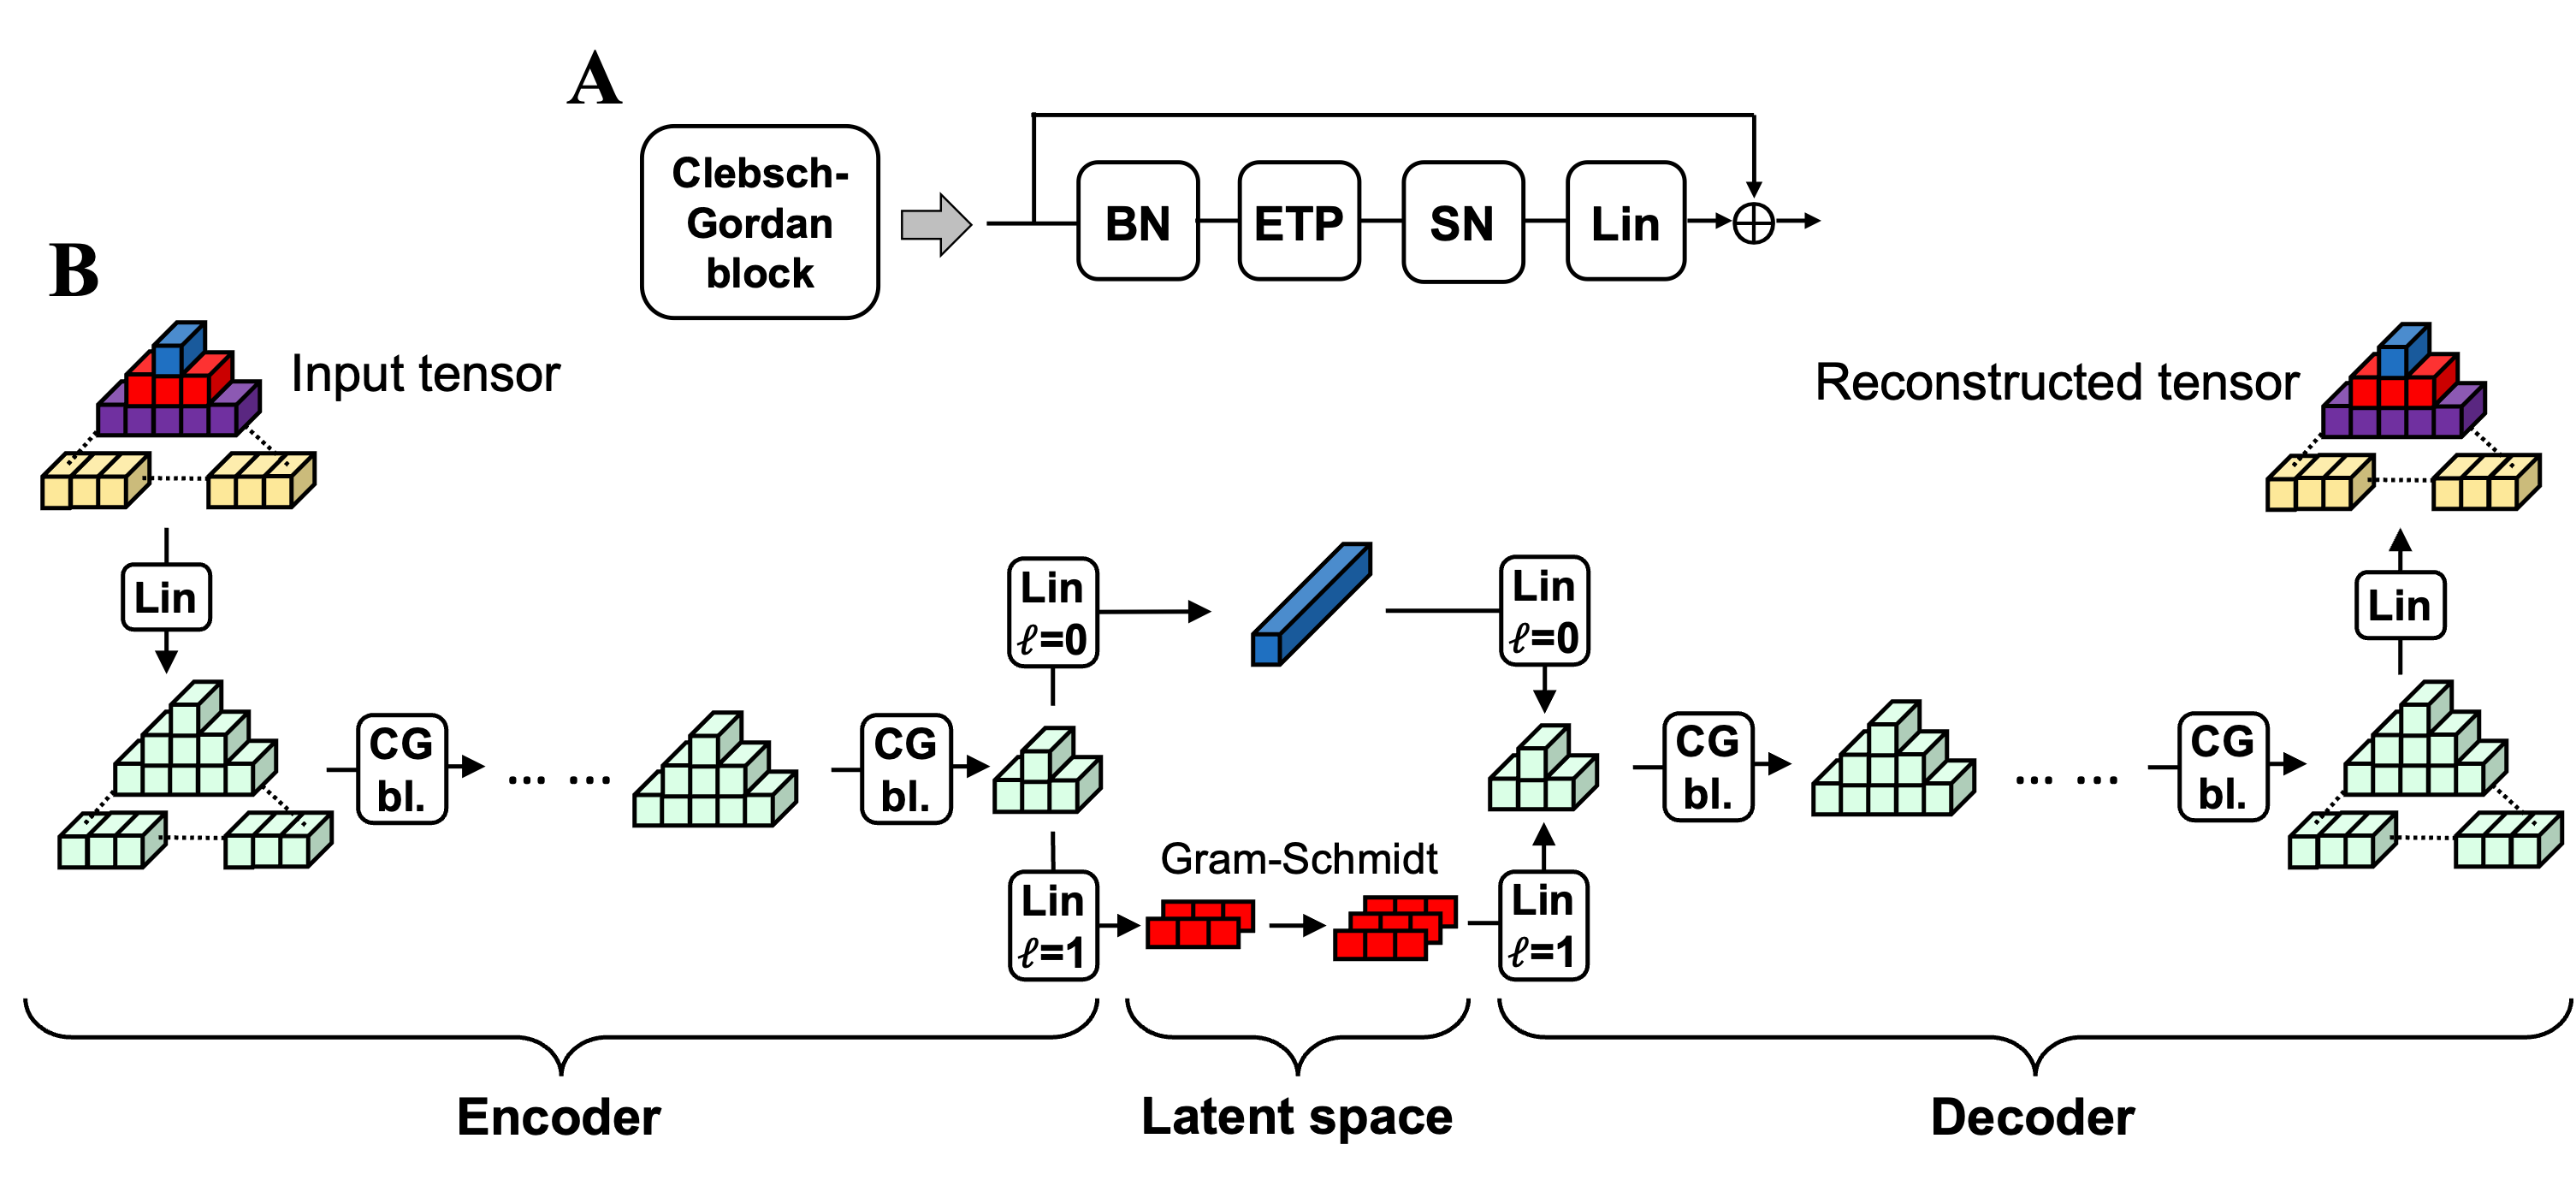
\includegraphics[width=0.9\textwidth]{figures/hvae_for_quals.png}
    \figcaption{Visualization of H-(V)AE's architecture.}{}
    \medskip
    \small
    \justifying
    \textbf{A:} Schematic of a Clebsch-Gordan Block (CG bl.), with batch norm (BN), efficient
    tensor product (ETP), and signal norm (SN), and Linear (Lin) operations. \textbf{B:} Schematic
    of the H-AE architecture. We color-code features of different degrees in the input and in the
    latent space for clarity. The H-VAE schematic differs only in the latent space, where two sets
    of invariants are learned (means and standard deviations of an isotropic Gaussian distribution).
    \label{fig:model}
\end{figure*}

\begin{figure*}[htbp]
    \centering
    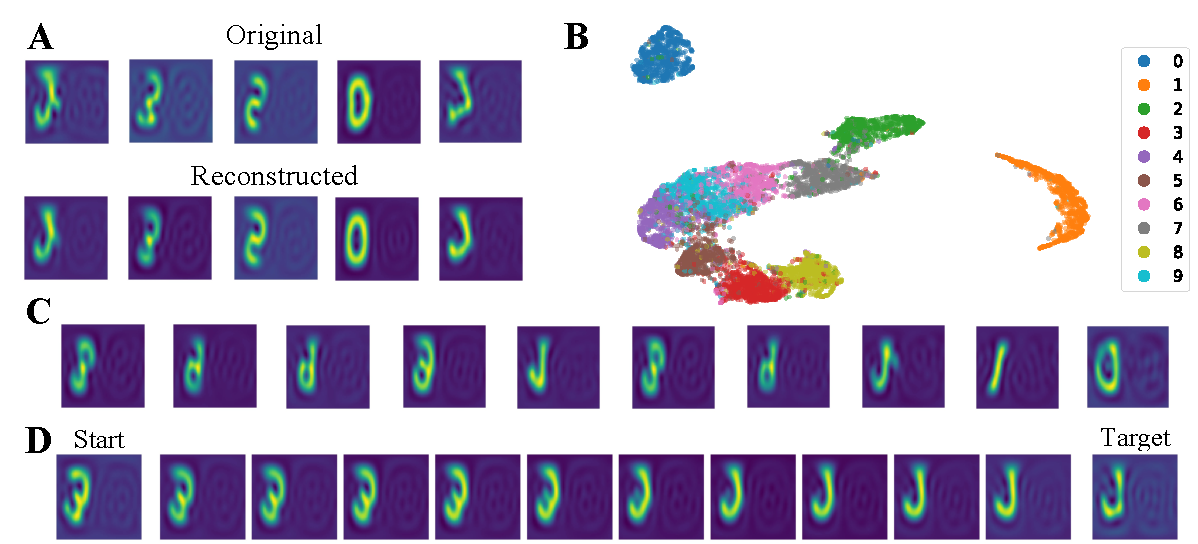
\includegraphics[width=0.83\textwidth]{figures/figure2_beta=0.6.pdf}
    \figcaption{H-VAE on MNIST-on-the-sphere.}{}
    \medskip
    \small
    \justifying
    Evaluation on rotated digits for an H-VAE trained on non-rotated digits with $z = 16$.
    \textbf{(A)} Original and reconstructed images in the canonical frame after inverse transform
    from Fourier space. The images are projected onto a plane. Distortions at the edges and
    flipping are side-effects of the projection. \textbf{(B)} visualization of the latent space via
    2D UMAP~\cite{mcinnes_umap_2020}. Data points are colored by digit identity. \textbf{(C)}
    Random images generated by feeding the decoder invariant embeddings sampled from the prior
    distribution and the canonical frame. See more examples in
    Figure~\ref{fig:mnist_samples_VAE_z_16_beta_0pt6}. \textbf{(D)} Example image trajectory by
    linearly interpolating through the learned invariant latent space.
    Interpolated invariant embeddings are fed to the decoder alongside the canonical frame. . See
    more examples in Figure~\ref{fig:mnist_trajectories_VAE_z_16_beta_0pt6}. MNIST-on-the-sphere
    dataset is created by projecting data from the planar MNIST on a discrete unit sphere, using
    the Driscoll-Healey (DH) method with a bandwidth (bw) of 30~\cite{cohen_spherical_2018}.
    \label{fig:mnist_viz}
\end{figure*}


\begin{figure*}
    \centering
    \resizebox{0.5\textwidth}{!}{
    \begin{tabular}{c}
        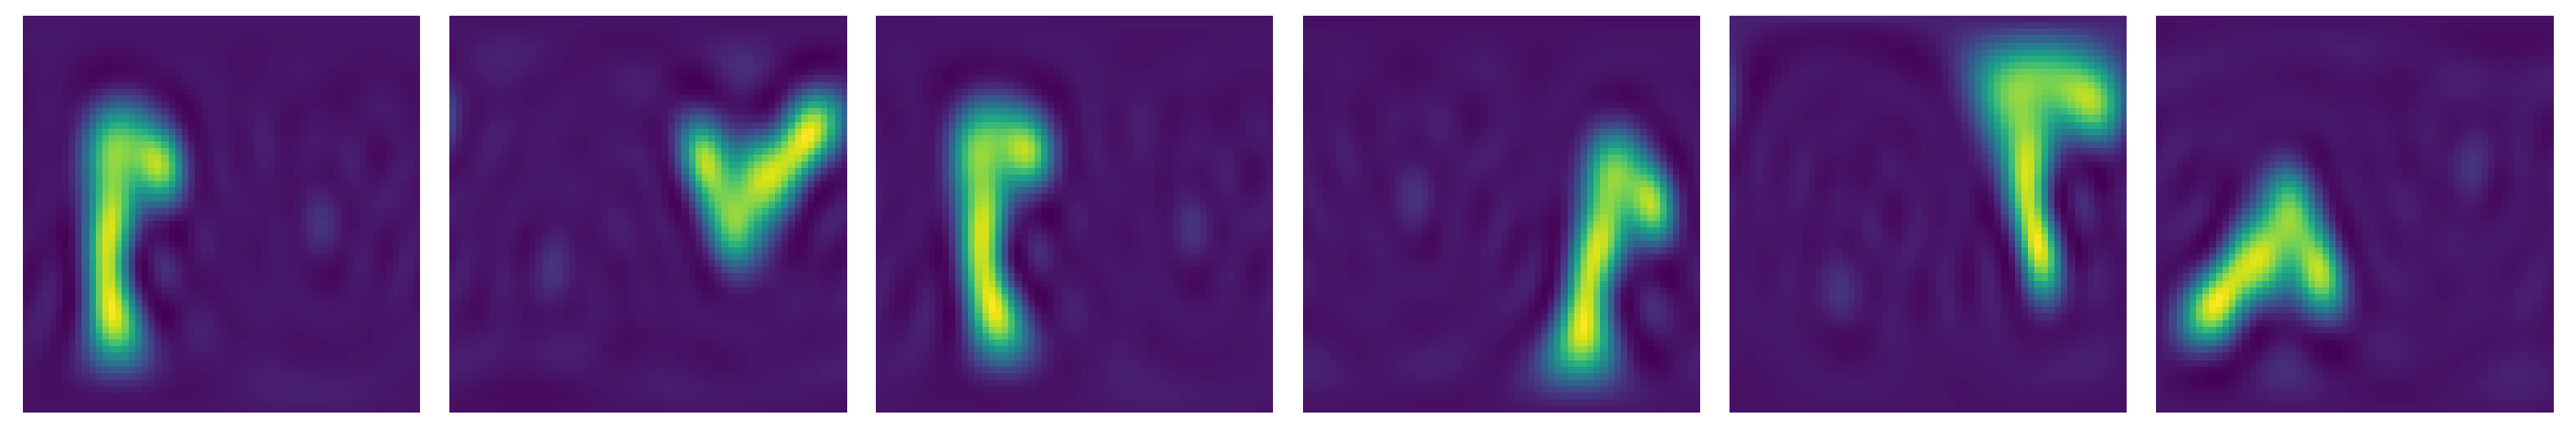
\includegraphics[width=0.8\textwidth]{figures/mnist/disentanglement/disentanglement-n_samples=1-seed=4.pdf}
        \\
        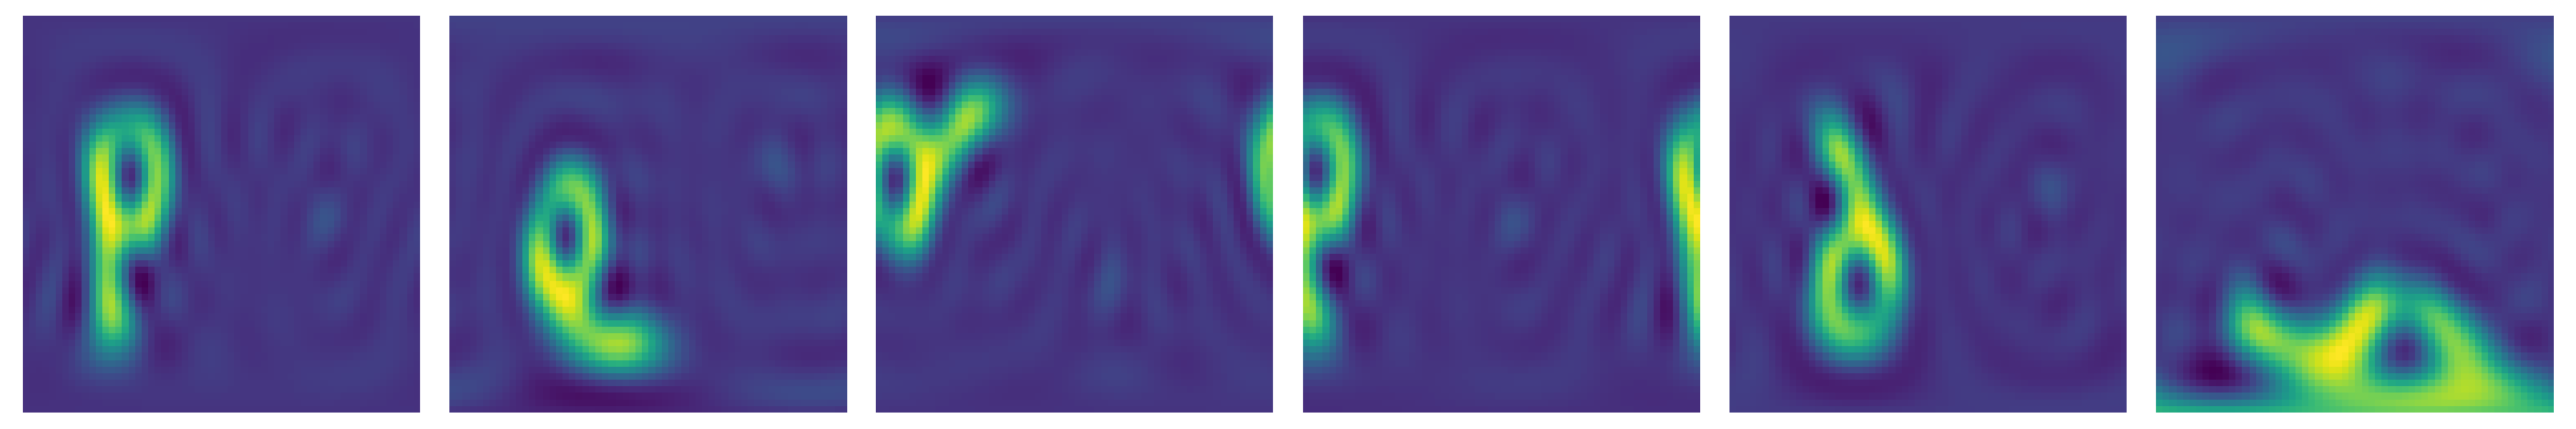
\includegraphics[width=0.8\textwidth]{figures/mnist/disentanglement/disentanglement-n_samples=1-seed=5.pdf}
        \\
        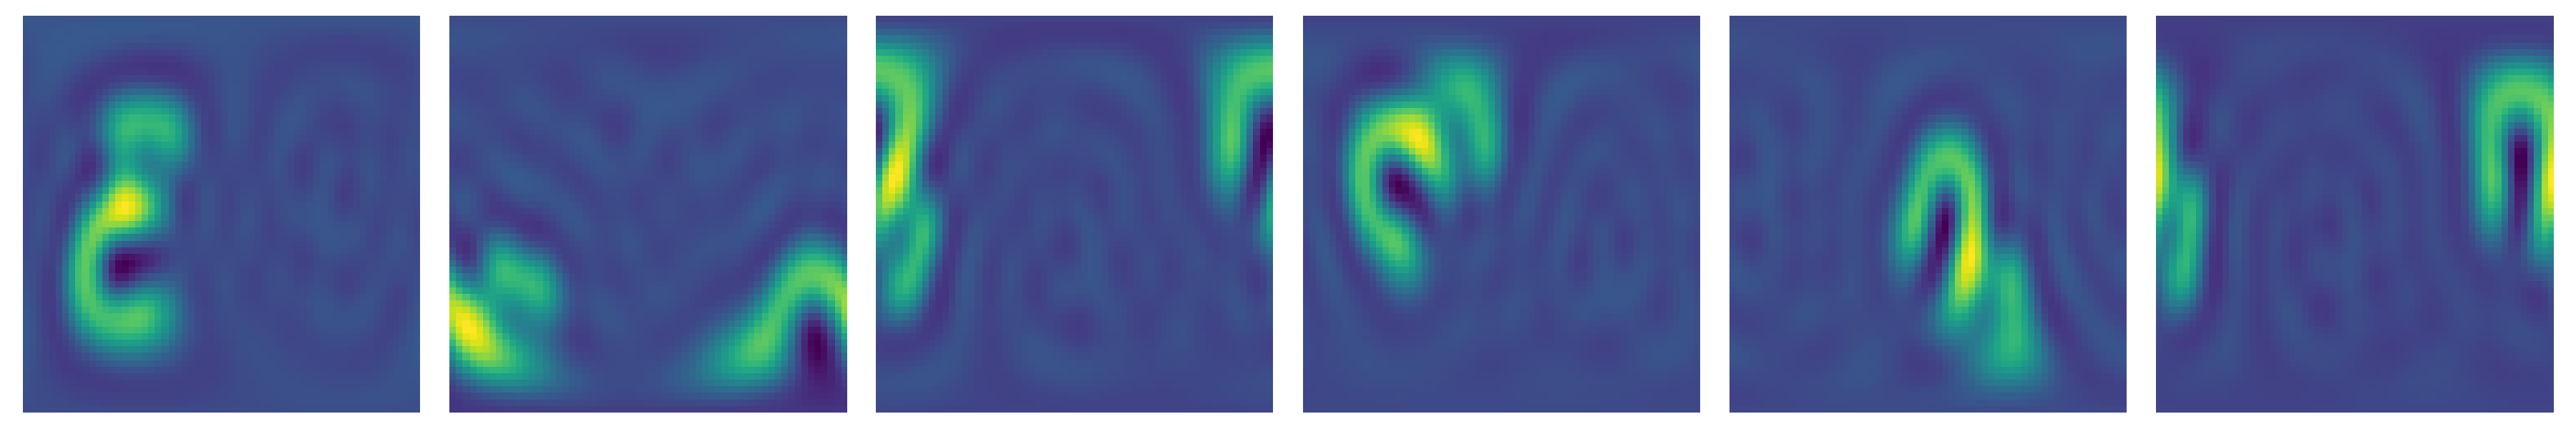
\includegraphics[width=0.8\textwidth]{figures/mnist/disentanglement/disentanglement-n_samples=1-seed=7.pdf}
    \end{tabular}
    }
    \figcaption{Visual evidence of the disentanglement in the latent space of
    MNIST-on-the-sphere.}{}
    \medskip
    \small
    \justifying
    For each row, the invariant embedding $\mathbf{z}$ is held fixed, and a different frame (i.e.,
    the rotation matrix) is used. Frames are sampled randomly and differ across rows, with the
    exception of the first column, where the frame is the same. Then, $\mathbf{z}$ and the frame
    are fed to the decoder and the Inverse Fourier Transform is used to generate the reconstructed
    spherical image, which is projected onto a plane for the ease of visualization. Modulo the
    distortions given by projecting the image onto a plane, it is clear that the invariant
    embedding contains all semantic information, and the frame solely determines the orientation of
    the image.
    \label{fig:disentanglement_mnist}
\end{figure*}


\section{Results}

\subsection{Rotated MNIST on the sphere}
\label{sec:mnist_results}
We extensively test the performance of  H-(V)AE on the MNIST-on-the-sphere
dataset~\cite{deng_mnist_2012}. Following ref.~\cite{cohen_spherical_2018}, we project the MNIST
dataset, which includes images of handwritten numbers,  onto the lower hemisphere of a discrete
unit sphere.
We consider two variants of training/test set splits, NR/R and R/R, differing in whether the
training/test images have been randomly rotated (R) or not (NR). For each dataset, we map the
images to steerable tensors via the Zernike Fourier Transform (ZFT) in Eq.~\ref{eq:ZFT} and train
models with different different sizes of latent spaces ($z=16$ vs. $z=120$) and model
types (AE vs. VAE). In all cases the model architecture follows from Figure~\ref{fig:model}C.\\
\\
For variational models, we tune the regularization strength $\beta$ such as to maximize
the expected quality of generated samples. We define samples to be of high quality if they 1) can
be correctly classified by a classifier trained on real data, and 2) if they are diverse enough,
finding that there is a trade-off between the two. We assess sample quality across $\beta$ by
generating them with conditional models and computing the accuracy of a classifier trained on real
data, as well as the variance of generated samples. We settle on $\beta$ values of $0.6$ and $2.8$
for the $z=16$ and $z=120$ models respectively, but also perform an ablation study and show that
the chosen values of $\beta$ are near-optimal according to quantitatie metrics on the quality of
the latent space (Figure~\ref{fig:ablation_in_beta_uncond}). See~\ref{sec:mnist_details} for more
details.


We use the metric {\em Cosine loss} to measure a model's reconstruction ability. Cosine loss is a
normalized dot product generalized to operate on pairs of steerable tensors (akin to cosine
similarity), and modified to be interpreted as a loss. Importantly, unlike MSE, Cosine loss is
dimensionless, and therefore, comparable across different datasets and encodings of data in tensors
of different sizes, though it is agnostic to magnitudes and thus unfit for training; see
Section~\ref{sec:cosine_loss_appendix} for details.

All trained models achieve very low reconstruction Cosine loss (Table~\ref{table:all_scores}) with
no significant difference between training modes, indicating that the models successfully leverage
SO(3)-equivariance to generalize to unseen orientations. Predictably, AE models have lower
reconstruction loss than VAE models (since they do not need to find a trade-off between
reconstruction error and KL divergence, Eq.~\ref{eqn:training_objective}), and so do models with a
larger latent space. Nonetheless, H-VAE achieves reliable reconstructions, as shown in
Figure~\ref{fig:mnist_viz}A and Table~\ref{table:all_scores}.

Interpretability of the latent space is also an important feature of a model.  All 8 models produce
an invariant latent space that naturally clusters by digit identity. We show this qualitatively for
four of the models in Fig.~\ref{fig:mnist_viz}B and
Fig.~\ref{fig:mnist_umaps}, and quantitatively by clustering the data via K-Means with 10
centroids and computing standard clustering metrics of Purity~\cite{aldenderfer_cluster_1984} and
V-measure~\cite{rosenberg_v-measure_2007} in Table~\ref{table:all_scores}.

Crucially, the built-in SO(3)-equivariance enables models trained on the non-rotated images to
seamlessly generalize to images that have been randomly rotated, as seen by the equivalent
performance between models trained and evaluated on the NR/R and R/R splits.



\begin{table*}
\begin{center}
\resizebox{\textwidth}{!}{
\begin{tabular}{l | l l c c | c | c c | c | c c c c c}
    \bf Dataset & \bf Type & \bf Method & \bf z & \bf bw & \bf \newlinecell{\bf Cosine} & \bf
    Purity & \bf V-meas. & \bf \newlinecell{Class.\\Acc.} & \bf P@N & \bf R@N & \bf F1@N & \bf mAP
    & \bf NDCG \\
    \hline
    \hline
    \multirow{11}{*}{MNIST}
    & \multirow{1}{*}{Supervised}
    & \cite{cobb_efficient_2021} NR/R      & - & 30 & - & - & - & 0.993 & - & - & - & - & - \\
    \cline{2-14}
    & \multirow{9}{*}{Unsupervised}
    & \cite{lohit_rotation-invariant_2020} NR/R      & 120 & 30 &      - & 0.40 & 0.35  & 0.894 & -
    & - & - & - & - \\
    & & H-AE NR/R (Ours)     & 120 & 30 & 0.017 & 0.59 &
    0.51 & 0.920 & - & - & - & - & - \\
    & & H-AE R/R (Ours)      & 120 & 30 & 0.015 & 0.65 &
    0.52 & 0.916 & - & - & - & - & - \\
    & & H-AE NR/R (Ours)     &  16 & 30 & 0.031 & 0.66 &
    0.55 & 0.850 & - & - & - & - & - \\
    & & H-AE R/R (Ours)      &  16 & 30 & 0.030 & 0.61 &
    0.52 & 0.844 & - & - & - & - & - \\
    & & H-VAE NR/R (Ours)    & 120 & 30 & 0.048 & \textbf{0.74} &
    \textbf{0.63} & \textbf{0.923} & - & - & - & - & - \\
    & & H-VAE R/R (Ours)     & 120 & 30 & 0.050 & 0.73 &
    0.60 & 0.916 & - & - & - & - & - \\
    & & H-VAE NR/R (Ours)    &  16 & 30 & 0.068 & 0.73 &
    0.60 & 0.878 & - & - & - & - & - \\
    & & H-VAE R/R (Ours)     &  16 & 30 & 0.067 & 0.69 &
    0.57 & 0.855 & - & - & - & - & - \\
    \hline
    \hline
    \multirow{5}{*}{Shrec17}
    & \multirow{2}{*}{Supervised}
    & \cite{esteves_spin-weighted_2020}     & - & 128 & - & - & - & - & 0.717 & 0.737 &   -   &
    0.685 &   -   \\
    & & \cite{cobb_efficient_2021}      & - & 128 & - & - & - & - & 0.719 & 0.710 & 0.708 & 0.679 &
    0.758 \\
    \cline{2-14}
    & \multirow{3}{*}{Unsupervised}
    & \cite{lohit_rotation-invariant_2020}        & 120 & 30 &     - & 0.41 & 0.34 & 0.578 & 0.351
    & 0.361 & 0.335 & 0.215 & 0.345 \\
    & & H-AE (Ours)       &  40 & 90 & 0.130 & 0.50 & 0.41 & \textbf{0.654} & \textbf{0.548} &
    \textbf{0.569} & \textbf{0.545} & \textbf{0.500} & \textbf{0.597} \\
    & & H-VAE (Ours)      &  40 & 90 & 0.151 & \textbf{0.52} & \textbf{0.42} & 0.631 & 0.512 &
    0.537 & 0.512 & 0.463 & 0.568 \\
\end{tabular}
}
\end{center}
    \figcaption{Performance metrics of H-(V)AE on MNIST-on-the-sphere and Shrec17.}{Reconstruction 
    Cosine loss, clustering metrics (Purity and V-measure), classification accuracy
    in the latent space using a linear classifier, and retrieval metrics (Shrec17 only) are shown. 
    For MNIST, we follow  ref.~\cite{cohen_spherical_2018}  to create the   MNIST-on-the-sphere
    dataset by   projecting data from the planar MNIST on a discrete unit sphere, using the
    Driscoll-Healey  method with a bandwidth (bw) of 30. We then map the images to steerable
    tensors via the Zernike Fourier Transform (ZFT) with $L = 10$, and a constant radial function
    $R^{n}_{\ell} = 1$, resulting in tensors with 121 coefficients. We train 8 models with
    different sizes of latent spaces $z$  (16 vs. 120) and model types (AE vs. VAE). 
    For Shrec17, we follow ref.~\cite{cohen_spherical_2018} and project surface information from
    each model onto an enclosing Driscoll-Healey spherical grid with a bandwidth of 90 via a
    ray-casting scheme, generating spherical images with 6 channels. We then apply the ZFT with $L
    = 14$ and a constant radial function $R^{n}_{\ell} = 1$ to each channel individually, resulting
    in a tensor with 1350 coefficients.
    We only report scores presented in the corresponding papers, and only the best-performing
    supervised method from the literature.}
\label{table:all_scores}
\end{table*}


All trained models achieve much better clustering metrics than Rot-Inv
AE~\cite{lohit_rotation-invariant_2020}, with the VAE models consistently outperforming the AE
models. We also train a linear classifier (LC) to predict digit identity from invariant latent
space descriptors, achieving better accuracy to Rot-Inv AE with the same latent space
size. We further observe marginal improvements of VAE over AE models in terms of
classification accuracy. Using a K-nearest neighbor (KNN) classifier instead of LC further
improves performance on the $z=16$ models (Table~\ref{table:mnist_scores_knn}). 

As H-VAE is a generative model, we generate random spherical images by sampling invariant latent
embeddings from the prior distribution, and observing diversity in digit type and style
(Fig.~\ref{fig:mnist_viz}C and
Fig.s~\ref{fig:mnist_samples_VAE_z_16_beta_0pt6},~\ref{fig:mnist_samples_VAE_z_120_beta_2pt8}). We
further assess the quality of the invariant latent space by generating images via linear
interpolation of the invariant embeddings associated with two test images. The interpolated images
present spatially consistent transitions (Fig.~\ref{fig:mnist_viz}D and
Fig.s~\ref{fig:mnist_trajectories_VAE_z_16_beta_0pt6},~\ref{fig:mnist_trajectories_VAE_z_120_beta_2pt8},
~\ref{fig:mnist_trajectories_AE_z_16}), which is a sign of a semantically well-structured latent space.

To understand the meaning of the learned frames, we ask ourselves what the output of the decoder
looks like if the frame is held constant; for simplicity, we set it equal to the $3 \times 3$
identity matrix. We experimentally find that the reconstructed elements tend to be aligned with
each other and hypothesize that the model is implicitly learning to maximize the overlap between
training elements, providing empirical evidence in Figure~\ref{fig:canonical_frames_1,7}. We call
this frame the \textbf{canonical} frame following the analogy with the canonical elements in
ref.~\cite{winter_unsupervised_2022}. We note that it is possible to rotate original elements to
the canonical frame thanks to the equivalence between the frame we learn and the rotation matrix
within our implementation; in fact in our experiments, when visualizing reconstructed or sampled
MNIST images, we first rotate them to the canonical frame for ease of visualization.




\subsection{Shrec17}

\begin{figure*}[t!]
   % \centering
    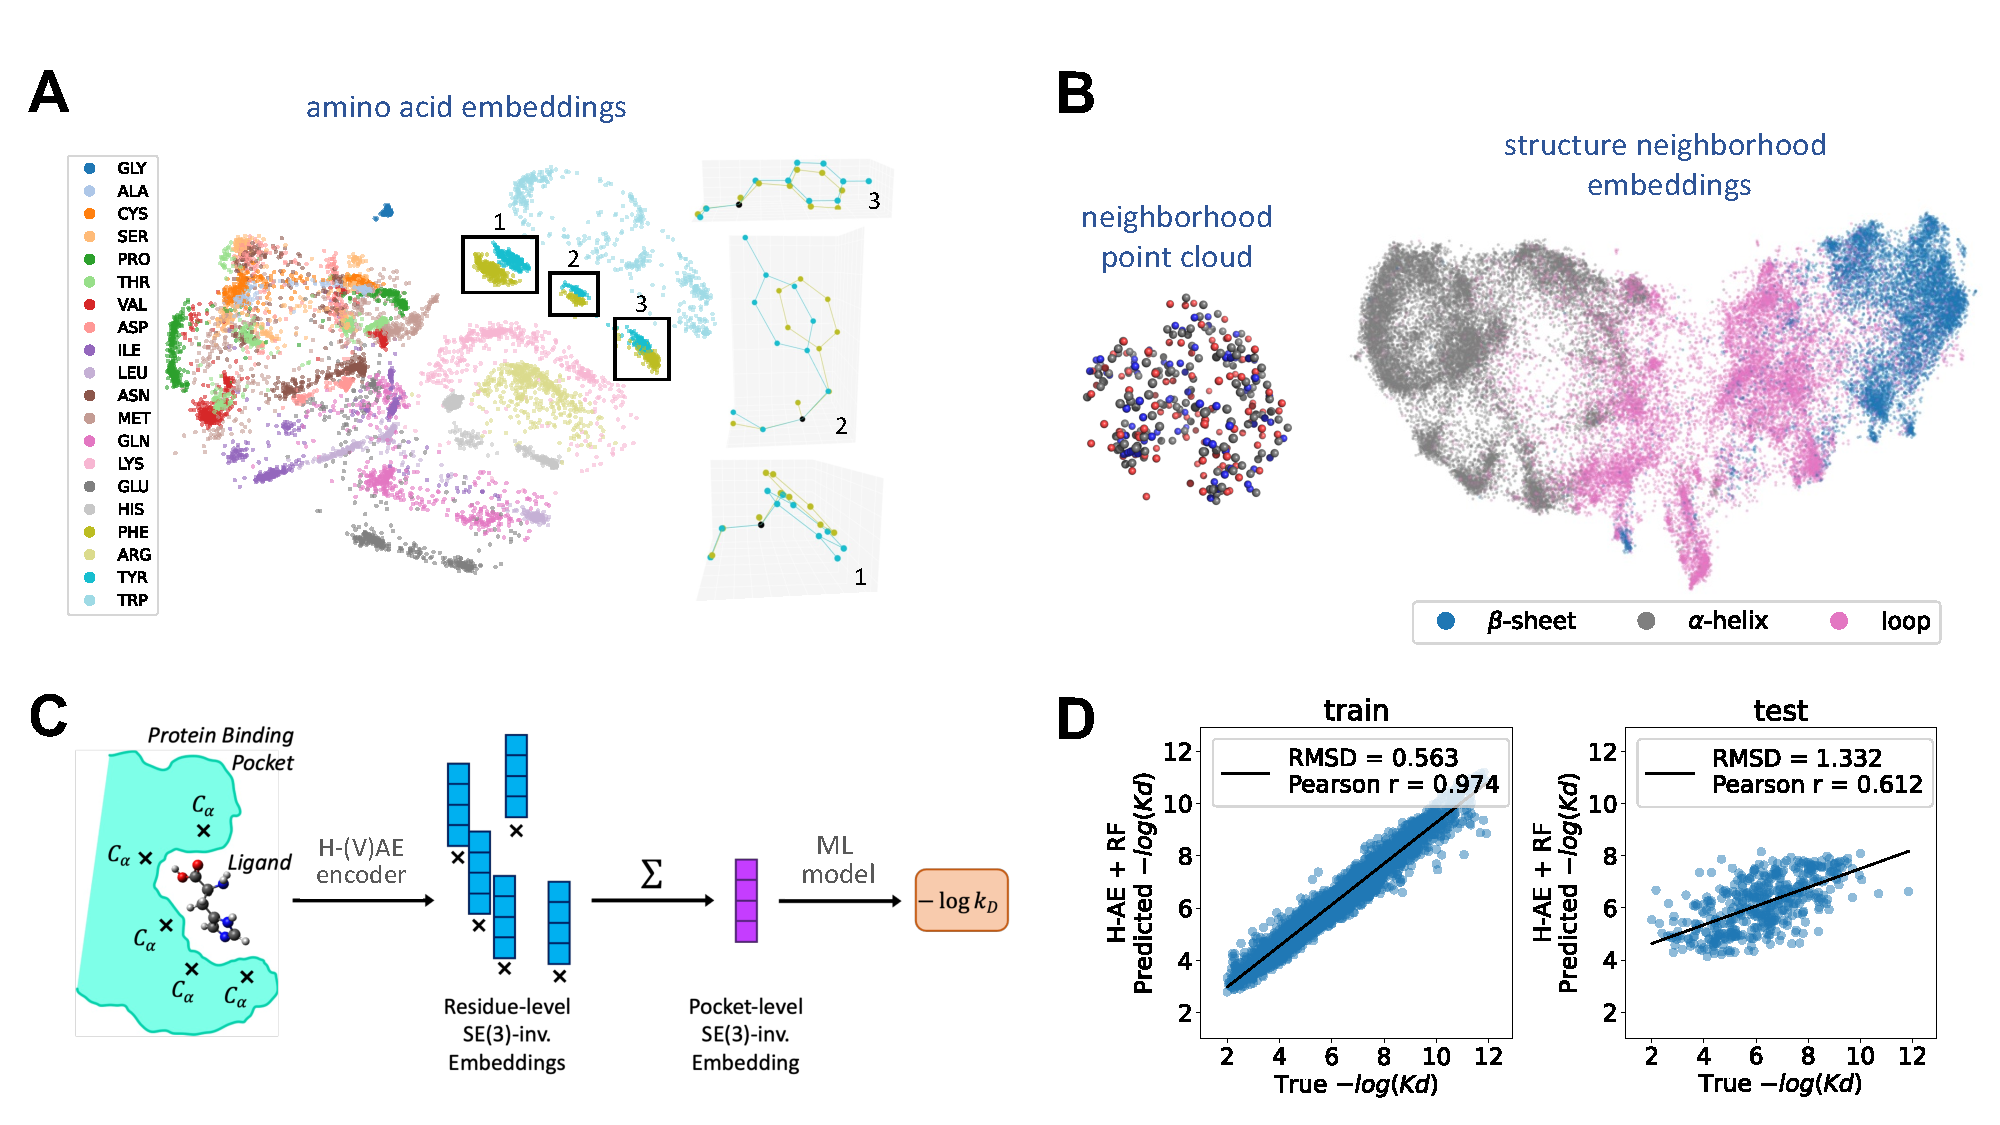
\includegraphics[width=\textwidth]{figures/protein_figure.pdf}\\
    \figcaption{Structural embeddings to predict protein-ligand binding affinities with H-(V)AE.}{
    \textbf{(A)}     H-VAE was trained to reconstruct the Fourier representation of 3D atomic point
    clouds representing amino acids (colors). The invariant latent space clusters by amino acid
    conformations. 
    The highlighted clusters for PHE and TYR contain residue pairs with similar conformations; TYR
    and PHE differ by one oxygen at the end of their benzene rings. We compare conformations by
    plotting each residue in the standard backbone frame (right); $x$ and $y$ axes are set by the
    orthonormalized C$\alpha$-N and C$\alpha$-C vectors, and $z$ axis is their cross product. For
    this plot, 1,000 amino acids were used as training data, with network parameters: $\beta =
    0.025$ and $z = 2$.     
    {\bf (B)} Left: An example protein neighborhood (point cloud of atoms) of 10 \AA\, around a
    central residue, used to train the H-AE models, is shown. Right: 2D UMAP visualization of the
    128-dimensional invariant latent space learned by H-AE trained on the protein structure
    neighborhoods with $L=6$ can separate neighborhoods by the secondary structure of their focal
    amino acid (colors); a linear classifier trained on 300,000 latent embeddings
    predicts secondary struvture of the focal amino-acid with 90\% accuracy. Each point represents
    a neighborhood. See Section~\ref{sec:protein_neighborhoods_details} for details on the
    network architecture and training procedure.
    {\bf (C)}  We use H-AE to extract the residue-level SO(3)-invariant embeddings in the binding
    pocket of a protein-ligand structure complex (data from PDBbind~\cite{su_comparative_2019}). We
    then sum over these embeddings to form an SE(3)-invariant pocket embedding that is used as an
    input to a standard Machine Learning model to predict the  binding affinity between the protein
    and the ligand.
    {\bf (D)} The predictions on the protein-ligand binding affinities from (C) is shown against
    the true values  for the training (left) and the test (right) sets. We use the data split
    provided by ATOM3D~\cite{townshend_atom3d_2021}, which devises training and test sets
    respectively containing 3507, and 490 protein-ligand complexes, with maximum 30\% sequence
    similarly between training and test proteins; see Table~\ref{table:lba_results} for a
    comparison against state-of-the-art methods.}
    \label{fig:lba_diagram}
\end{figure*}


The Shrec17 dataset consists of 51k colorless 3D models belonging to 55 object classes, with a
70/10/20 train/valid/test split~\cite{noauthor_shrec_nodate}. We use the variant of the dataset in
which each object is randomly rotated. Converting 3D shapes into spherical images preserves
topological surface information, while significantly simplifying the representation. We follow
ref.~\cite{cohen_spherical_2018} 
and project surface information for each image onto an enclosing spherical grid via a ray-casting
scheme and apply ZFT (eq.~\ref{eq:ZFT}) on these transformed images.

We train an AE and a VAE model on ZFT transformed data (Section~\ref{sec:shrec17_details}) and,
similarly to the MNIST dataset, compute cosine loss, clustering metrics and classification
accuracy via a linear classifier. We also compute the standard Shrec17 object retrieval metrics via
the latent space linear classifier's predictions (see~\cite{noauthor_shrec_nodate} for a
description of the retrieval metrics). H-AE achieves the best classification and retrieval results
for autoencoder-based models, and is competitive with supervised models despite the lower grid
bandwidth and the small latent space (Table~\ref{table:all_scores}). Using KNN classification
instead of a linear classifier further improves performance
(Table~\ref{table:shrec17_evaluation_knn}). H-VAE achieves slightly worse classification results
but better clustering metrics compared to H-AE. While reconstruction loss is low, there is still
significant margin of improvement. 

\subsection{Structural  embeddings of amino acid neighborhoods to predict function}
Here, we provide a strong use case for H-(V)AE in structural biology. 
Specifically, we learn expressive embeddings for amino acids neighborhoods within protein
structures that can be used to learn protein function.\\

\noindent {\bf \small Embeddings of amino acid conformations.}  As a first, propedeutic step, we
train H-(V)AE to reconstruct the 3D structure of individual amino acids, represented as atomic
point clouds, extracted from protein structures in the Protein Data Bank
(PDB)~\cite{berman_protein_2000}. Residues of the same type have different conformations and
naturally have noisy coordinates, making this problem a natural benchmark for our rotationally
equivariant method. 

We represent an amino acid by atom-type-specific clouds (C, O, N and S; we exclude H) centered at
the residue's C$\alpha$ and compute the ZFT (eq.~\ref{eq:ZFT}) with $L = 4$ and $N = 20$ within a
radius of $10$\AA\, from the residue's C$\alpha$, and concatenate features of the same degree
$\ell$, resulting in a tensor with 940 coefficients. We train several H-AE and H-VAE with different
architectures, but all with the latent space sizes $z=2$; see Sec.~\ref{sec:toy_aminoacids_details}
for details.\\ 


We consistently find that the latent space clusters by amino acid conformations
(Figure~\ref{fig:lba_diagram}A), with sharper cluster separations as more training data is added
(Figure~\ref{fig:toy_aminoacids_data_ablation_umap_AE}
and~\ref{fig:toy_aminoacids_data_ablation_umap_VAE}). We find that test reconstruction loss
decreases with more training data but the reconstruction is accurate even with little training data
(from 0.153 Cosine loss with 400 training residues to 0.034 with 20,000); 
Table~\ref{table:toy_aas_data_ablation_z_eq_2}. A similar trend is observed for KNN-based
classification accuracy of residues (from 0.842 with 400 training residues to 0.972 with 20,000);
(Table~\ref{table:toy_aas_data_ablation_z_eq_2}). Notably, an untrained model, while achieving
random reconstruction loss, still produces an informative invariant latent space (0.629 residue
type accuracy), suggesting that the forced SO(3)-invariance grants a ``warm start" to the encoder.
We do not find significant improvements in latent space classification by training with a
variational objective, and present ablation results in
Table~\ref{table:toy_aas_kld_ablation_z_eq_2}.\\



\noindent {\bf  \small Embeddings of amino acid structure neighborhoods.}  The structural
neighborhood surrounding an amino acid provides a context for its function (e.g., whether it takes
part in interaction with other proteins at a protein-protein interface or not). Indeed, our
previous work has shown that supervised learning algorithms can accurately classify focal amino
acids based on the composition of their surrounding neighborhoods~\cite{pun_learning_2022}. Here,
we  train H-(V)AE to reconstruct residue-specific protein \textit{neighborhoods} - which we define
as the point clouds of atoms within 10\AA\, of a residue's C$\alpha$ - across the protein universe
(Fig.~\ref{fig:lba_diagram}A).  We extract these protein neighborhoods from all proteins in
ProteinNet~\cite{alquraishi_proteinnet_2019}. We then construct each neighborhood's Fourier
representation by computing the ZFT (Eq.~\ref{eq:ZFT}) over the point clouds associated with each
atom type within the neighrbohood (C, N, O and S) and concatenating atom-specific features of the
same degree $\ell$.

We train several H-AE models with varying architectures with different maximum spherical degree $L$
and latent space sizes $z$ (see details in Sec.~\ref{sec:protein_neighborhoods_details}); note that
we do not experiment with variational models for this task. H-AE shows strong reconstruction
ability, but its accuracy worsens with smaller latent space sizes and higher maximum spherical
degree $L$ (Table~\ref{table:mse_and_cosine}).
Notably, the learned latent space is smoothly structured according to geometric
features of the neighborhoods, such as the presence of secondary structure components
(Fig.~\ref{fig:lba_diagram}B and~\ref{fig:umaps_sec_struct_with_abundances}) and number of atoms
(Figure~\ref{fig:umap_total_power}).




\begin{table}[t]
\begin{center}
\resizebox{0.6\textwidth}{!}{
\begin{tabular}{l | c c c}
     & \multicolumn{3}{c}{\newlinecell{\textbf{Ligand Binding Affinity}\\\textbf{30\% Similarity}}}
     \\
    {Model} & {RMSD $\downarrow$} & {Pearson's r $\uparrow$} & {Spearman's r $\uparrow$} \\
    \hline
    DeepDTA &                  $1.565$           & $0.573$           & $0.574$           \\ 
    3DCNN &                    $1.414 \pm 0.021$ & $0.550$           & $0.553$           \\
    GNN &                      $1.570 \pm 0.025$ & $0.545$           & $0.533$           \\
    MaSIF &                    $1.484 \pm 0.018$ & $0.467 \pm 0.020$ & $0.455 \pm 0.014$ \\
    EGNN &                     $1.492 \pm 0.012$ & $0.489 \pm 0.017$ & $0.472 \pm 0.008$ \\
    GBPNet &                   $1.405 \pm 0.009$ & $0.561$           & $0.557$           \\
    EGNN + PLM &               $1.403 \pm 0.013$ & $0.565 \pm 0.016$ & $0.544 \pm 0.005$ \\
    ProtMD  &                  \underline{$1.367 \pm 0.014$} & \underline{$0.601 \pm 0.036$} &
    \underline{$0.587 \pm 0.042$}\\
    \hline
    H-AE + L.R. & $1.397 \pm 0.019$ & $0.560 \pm 0.017$ & $0.568 \pm 0.018$ \\
    H-AE + R.F. &     $\mathbf{1.332 \pm 0.012}$ & $\mathbf{0.612 \pm 0.009}$ & $\mathbf{0.619 \pm
    0.009}$
\end{tabular}
}
\end{center}
    \figcaption{Results on the Ligand Binding Affinity task.}{Prediction accuracies using H-AE
    embeddings with  Linear Regression (L.R.), and  Random Forest (R.F.) Regression are benchmarked
    against other methods. We choose the H-AE model with best RMSD on validation split, which is the
    model with $L = 6$ and $z = 128$ for both Linear Regression and Random Forest. For each set of
    predictions, we use an ensemble of 10 Regressors as we noted a small but consistent improvement
    in performance. Best scores are in \textbf{bold} and second-best scores are \underline{underlined}.
    H-AE+R.F. delivers state-of-the-art predictions. Methods are ordered by date of release;
    see Table~\ref{table:lba_results_appendix} for more details.}
\label{table:lba_results}
\end{table}




\noindent {\bf \small Predicting protein-Ligand Binding Affinity (LBA).}  The binding interaction
between proteins and ligands should be primarily determined  by the composition of the protein's
binding pocket in complex with the ligand. Therefore, we hypothesized that the inferred protein
structure  embeddings  (Fig.~\ref{fig:lba_diagram}B) should contain information about
protein-ligand binding interactions, if the neighborhood is defined along the binding pocket and
contains atoms from the ligand. To test this hypothesis, we  follow the pipeline in
Fig.~\ref{fig:lba_diagram}C. Specifically,  given a protein-ligand structure complex, we identify
residues in the binding pocket (i.e., residues with C-$\alpha$ within 10\AA\, of the ligand) and
extract their structure neighborhoods, which include atoms from both the protein and the ligand. We
then pass the residue-centered neighborhoods of the binding pocket through a trained H-AE's encoder
to extract their rotationally-invariant embeddings. We highlight that, since the neighborhood
centers are well-defined at the residues' C-$\alpha$'s, the embeddings are not only rotationally
invariant about their center, but also translationally invariant with the respect to translations
of the whole system, i.e., they are effectively SE(3)-invariant. 

Since protein-ligand binding affinity is an extensive quantity in the number of interacting
residues, we construct a pocket embedding by summing over residue-level embeddings; the resulting
pocket embedding is SE(3)-invariant, reflecting the natural symmetry of the LBA task. We use these
pocket embeddings as feature vectors to train simple Machine Learning models to predict
protein-ligand binding affinities. 


To test the performance of our method, we use the LBA dataset in
ATOM3D~\cite{townshend_atom3d_2021} that provides the PDB structure of the protein-ligand complex
together with   either the measured dissociation constant $K_d$ or the inhibition constant $K_i$;
see Sec.~\ref{sec:lba_details} for further details. To map between the learned pocket embeddings to
the log dissociation (or inhibition) constants we train both a simple Linear and a Random Forest
Regressor on a training sets provided by ATOM3D.  Fig.~\ref{fig:lba_diagram}D shows the performance
of the model with the Random Forest Regressor and Table~\ref{table:lba_results} provide a detailed
benchmark of our methods against prior approaches.  The Linear model achieves competitive results,
whereas the Random Forest Regressor achieves state-of-the-art. 

These results demonstrate the utility of unsupervised learning for residue-level protein structure
representations in predicting complex protein functions. Most of the competing structure-based
methods for LBA (Table~\ref{table:lba_results}) learn complex graph-based functions on top of
simple atomic representation, whereas our method uses simpler machine learning models over rich
residue-level representations. Notably, ProtMD (the method competitive to ours) performs a
pre-training scheme using expensive molecular dynamics simulations that informs the model about
conformational flexibility, information that our method does not have access to. Given the
computational cost of training complex atom-level graph-based models, our residue-based approach
can offer a more viable alternative for modeling large protein interfaces.


\section{Summary}

In this chapter, we have developed the first end-to-end SO(3)-equivariant unsupervised algorithm, termed Holographic
(Variational) Auto-Encoder (H-(V)AE), suitable for data distributed in three dimensions around a given central point.
The model learns an invariant embedding describing the data in a ``canonical" orientation alongside an equivariant frame
describing the data's original orientation relative to the canonical one.

Prior works have attempted to learn representations that are invariant to certain transformations. For example, in
refs.~\cite{shu_deforming_2018, koneripalli_rate-invariant_2020} general ``shape" embeddings are learned by
characterizing a separate ``deformation" embedding. However, these networks are not explicitly equivariant to the
transformations of interest.

Others proposed to learn an exactly invariant embedding alongside an approximate (but not equivariant) group action to
align the input and the reconstructed data. For example, {\em Mehr et al}~\cite{mehr_manifold_2018} learns in
quotient space by pooling together the latent encodings of copies of the data that have been transformed with sampled
group actions, and backpropagate the minimum reconstruction loss between the decoded element and the transformed copies
of the data. This approach is best suited for discrete and finite groups, for which it does not require approximations,
and it is computationally expensive as it is akin to data augmentation. {\em Lohit et
al}~\cite{lohit_rotation-invariant_2020} construct an SO(3)-invariant autoencoder for spherical signals by learning an
invariant latent space and minimizing a loss which first finds the rotation that best aligns the true and reconstructed
signals. Although this approach is effective for non-discrete data, it still manually imposes rotational invariance, and
can only reconstruct signals up to a global rotation. In contrast, H-(V)AE is fully equivariant and only requires simple
MSE for reconstruction of data in its original orientation.

A small body of work went beyond invariance to develop equivariant autoencoders. Several methods construct data and
group-specific architectures to auto-encode data equivariantly, learning an equivariant representation in the
process~\cite{hinton_transforming_2011, kosiorek_stacked_2019}. Others use supervision to extract class-invariant and
class-equivariant representations~\cite{feige_invariant-equivariant_2022}. A recent theoretical work proposes to train
an encoder that encodes elements into an invariant embedding and an equivariant group action, then using a standard
decoder that uses the invariants to reconstruct the elements in a canonical form, and finally applying the learned group
action to recover the data's original form~\cite{winter_unsupervised_2022}. Our method in SO(3) is closely related to
this work, with the crucial difference that our network is end-to-end rotationally equivariant, in that we use an
equivariant decoder and learn to reconstruct the Fourier encoding of the data. A more detailed comparison of the two
approaches and the benefits of our fully equivariant approach can be found in the Appendix
(Section~\ref{sec:mlp_decoder_appendix}) and in Table~\ref{table:mlp_decoder_comparison}.
Recently, generative models of atomic point clouds that are equivariant to Euclidean transformation have been developed
for molecular~\citep{hoogeboom_equivariant_2022} and protein~\citep{yim_se3_2023, watson_broadly_2022} generation in
3D using Normalizing Flows~\citep{hoogeboom_equivariant_2022} and diffusion processes~\citep{satorras_en_2022,
yim_se3_2023, watson_broadly_2022}. Our work is partly related to these, but with some crucial differences. 1) Our
method is designed for spherical images and for point clouds with a preferential center, as opposed to point clouds. 2)
The use of an autoencoder architecture makes our method suitable for compressing information into a lower-dimensional
space, for effective later use in annotation-scarce domains like ligand binding affinity prediction; by contrast the
latent space of normalizing flows and diffusion-based models must have the same size as the data, making them unsuitable
for this task.

There is also a diverse body of literature on constructing representations of atomic systems that are
invariant/equivariant to euclidean symmetries, leveraging Fourier transforms and CG tensor products, with focused
applications on materials science~\cite{drautz_atomic_2019, musil_physics-inspired_2021, uhrin_through_2021}\\

H-(V)AE's learned embeddings are highly expressive. For example, we used the learned invariants to achieve
state-of-the-art unsupervised clustering and classification results on various spherical image datasets. By making our
model variational in its invariant latent space, we enhanced the quality of clustering and made the model generative.
Our model is defined fully in spherical Fourier space, and thus, can reach a desired expressiveness without a need for
excessive computational resources.

H-(V)AE also produces rich residue-level representations of local neighborhoods in protein structures, which we use as
embeddings for downstream structure-based tasks such as Ligand Binding Affinity prediction. Indeed, H-(V)AE
representations paired with a simple Random Forest Regressor achieve state-of-the-art results on learning the binding
affinity between proteins and small molecule ligands.

More broadly, we expect that H-(V)AE can be used to extract rich, symmetry-aware features from local neighborhoods in
spherical images and complex 3D objects, to be used in more complex downstream tasks that benefit from the symmetry
constraints. For example, our method can be leveraged for modeling diffusion MRI data, for which rotation-equivariant
methods have recently shown to be highly beneficial~\cite{muller_rotation-equivariant_2021}. In structural biology, we
expect our method to be useful for coarse-graining full-atom representations of protein structures to facilitate
structure-based predictions of protein function. For example, a large protein graph can be coarse-grained by
substituting its full-atom representation with rich embeddings of local structural neighborhoods learned from an
unsupervised model. With an added supervised step, these coarse-grained embedding can be leveraged to predict complex
protein functions, as we show for predicting ligand binding affinity. This approach is akin to using protein
embeddings for sequence data, learned by language models, to inform (few-shot) predictions for protein
function~\cite{swanson_predicting_2022}.




\chapter{H-Packer: Holographic Packer}
\label{sec:hpacker}

The contents of this chapter are published in~\citet{visani_h-packer_2024}, under the title
\textit{H-Packer: Holographic Rotationally Equivariant Convolutional Neural Network for Protein
Side-Chain Packing}.

Determining amino acid side-chain conformations in a protein, known as Protein Side-Chain Packing
(or Rotamer Packing), is an essential step in protein folding and the de-novo design of proteins.
Computational approaches to protein folding often divide the structure inference problem into two
steps: first, they characterize the rigid backbone structure, and then they pack the side-chains
associated with the amino acids at each residue. The flexibility of the side-chain makes the search
in the space of possible conformations inevitably complex and computationally expensive. The
de-novo protein design protocols also rely on similar logical steps: often an amino acid sequence
compatible with a desirable backbone structure is to be inferred
(designed)~\citep{dauparas_robust_2022} and then the associated side-chains should be packed to
form the full atomic composition of a protein. Furthermore, it has been suggested that models
trained to learn \textit{distributions} of side-chain conformations can be used to predict
mutational effects in a zero-shot fashion~\citep{luo_rotamer_2023}, thereby making rotamer packing
a valuable proxy problem for resolving structure-to-function maps.

Many of the conventional methods for side-chain packing rely on physical models through which they
find a rotamer that minimizes a physically-reasoned heuristic energy of the protein
fold~\citep{alford_rosetta_2017, huang_faspr_2020, krivov_improved_2009,
cao_improved_2011, liang_fast_2011}. Popular algorithms include RosettaPacker from the rosetta
suite~\citep{alford_rosetta_2017}, FASPR~\citep{huang_faspr_2020}, and
SCWRL~\citep{krivov_improved_2009}.
However, these computational methods often lack accuracy and speed in their predictions.
As deep learning makes
strides in protein science, there is a growing effort in developing machine learning methods for
rotamer packing. Among these methods is DLPacker~\citep{misiura_dlpacker_2022}, which treats the
packing problem as an image transformation. This algorithm characterizes the local environment of a
given amino acid backbone within a structure as a 3D image, and uses this model to predict the
atomic coordinates of the side chain. It then compares the predicted side-chain to a pre-set
library of rotamers to select the closest conformation. AttnPacker~\citep{mcpartlon_end--end_2023},
a more recently developed method, uses a deep graph attention network to model the local geometry
of a residue within a structure and is trained to predict the coordinates of the side-chain atoms.
Recently, diffusion models over side-chain torsional angles have also being applied, such as
DiffPack~\citep{zhang_diffpack_2023}.

The specific conformation - or the ensemble of conformations - adopted by a side-chain is fundamentally
determined by the physical forces acting upon it, among which those coming from local sources are the
most prominent. Therefore, modeling a side-chain's conformation as a function of its local atomic environment
is a physics-appropriate approximation. Furthermore, the conformation can be described unambiguously by 
SO(3)-invariant or SO(3)-equivariant variables. Thus, side-chain packing fits nicely within our framework of
rotationally equivariant modeling of residue-centered protein neighborhoods.

Here, we tackle the problem of side-chain packing by learning to directly regress over $\chi$
(torsional) angles, which are main degrees of freedom determining side-chain conformations. We
derive and discuss three possible parameterizations of the $\chi$ angles, ultimately settling on
regressing over the Sine and Cosine transforms of the angles, which are rotationally invariant. We
introduce Holographic-Packer (H-Packer), a deep learning method that packs rotamers by first
predicting candidate $\chi$ angles from backbone and sequence, and then refines the predictions
with a model trained on full-atom structures.

By directly predicting the side-chain $\chi$-angles, H-packer does not rely on comparing its output
with a pre-set library of rotamers, making it computationally more efficient than methods like
DLPacker. Furthermore, H-Packer is light-weight (2$\times$3M parameters vs. 208M of AttnPacker) and
requires few resources to train (single vs. multiple GPUs for diffusion models like DiffPack). We
evaluate the packing performance of H-Packer on standard datasets, and show that it has generally
better performance than conventional physics-based methods, and competitive against machine
learning solutions. In general, our results suggest that H-Packer has learned complementary
features to alternative methods.
Code for H-Packer is freely available at \texttt{https://github.com/gvisani/hpacker}.



\section{Methods}

\subsection{Modeling side-chain conformations with $\chi$ Angles}

While amino acids are composed of a maximum of 10 heavy atoms (in the case of Tryptophan), their 3D
conformations can be uniquely described by the value of at most 4 dihedral angles, referred to as
the $\chi$ angles (Figure~\ref{fig:hpacker}A). This reduction in the number of degrees of freedom
is granted due to the physical constraints posed on the remaining internal coordinates (bond
angles, bond lengths, and dihedral angles - \textit{redundant internal coordinates}). Specifically,
the inter-atomic physical interactions within amino acids often constrain these redundant
coordinates to a constant, or a well-defined function of the residue's $\chi$ angles. Therefore,
predicting $\chi$ angles is the key step in side-chain packing.

H-packer addresses the side-chain packing problem in two steps: (i) it predicts the value of $\chi$
angles, and (ii) it reconstructs the atomic coordinates using the predicted $\chi$ angles and the
constrained values of the redundant internal coordinates. Specifically, we evaluate the redundant
internal coordinates from a subset of training data (1,700 structures) by leveraging the
\texttt{internal\_coords} feature of the \texttt{biopython} package. We empirically verified that
the distributions of values were Gaussian with low variance, and resolved to take their
\textit{medians} as the ground truth. Substituting these values for the original ones yields a
negligible Null Reconstruction error of approximately
0.127\AA\,(Figure~\ref{fig:null_reconstruction}). Notably, this error remains unchanged even when
using only 100 reference structures instead of 1,700
(Figure~\ref{fig:null_reconstruction_comparison}).

\subsection{Predicting $\chi$ angles using H-Packer}
We aim to predict the $\chi$ angles associated with a side-chain conformation from the
configuration of atoms surrounding a given residue. This atomic neighborhood is associated with the
backbone and the side-chain of the neighboring residues in the structure.

During inference only the coordinates of the backbone atoms are known a priori - alongside the
identity of the amino acids they belong to. However, physical interactions with the atoms of
neighboring side-chains are the true determinants of a residue's conformation. Therefore, we
develop H-Packer into a two-step solution (Figure~\ref{fig:hpacker}C). Specifically, we two train
models: one to predict $\chi$ angles from the backbone atoms and amino-acid identity alone, the
another to predict $\chi$ angles from full neighborhoods, i.e., by including the true side-chain
atoms of the surrounding residues (minus the residue of interest). At inference time, we use the
first model to make an \textit{initial guess} of the side-chain conformations, and then a second
model to iteratively \textit{refine} the predictions.

To build the individual models that predict $\chi$ angles, we start by considering their
symmetries. Notably, $\chi$ angles are \textit{invariant} to rigid-body transformations
(translations and rotations) of the protein (i.e., they are SE(3) invariant). Translation
invariance can be satisfied by choosing a well-defined center for a residue of interest (e.g. the
residue's C$\alpha$), leaving rotational (i.e. SO(3) invariance) about the chosen center to be
accounted for. The rotational symmetry and the dependence on local interaction make this problem
fall neatly within our framework of SO(3)-equivariant modeling of protein neighborhoods. Thus we
build two SO(3)-equivariant models - using the components described in Chapter~\ref{sec:background}
- to predict a residue's $\chi$ angles, considering as input the point cloud of atoms within a
radius $r=10\AA$ of the residue's C-$\alpha$ (with or without the neighboring side-chains).


\begin{figure}[t]
    \centering
    \resizebox{1.0\textwidth}{!}{
    
\includegraphics{Quals/figures/hpacker.pdf}
    }
    \figcaption{Overview of H-Packer.}{}
    \medskip
    \small
    \justifying
    \textbf{A:} Illustration of Glutamine's $\chi$ angles, of which there are three. \textbf{B:}
    Schematic shows the SO(3)-Equivariant network for side-chain packing by first predicting the
    missing residue's $\chi$ angles from its surrounding atomic environment, and then using the
    $\chi$ angles to reconstruct the residue's side-chain. As illustrated in \textbf{C}, H-Packer
    consists of two networks, one trained on backbone atoms only and used to make an initial guess,
    and one trained on full side-chain neighborhoods and used to refine the predictions.
    \label{fig:hpacker}
    % \vspace{-4mm}
\end{figure}


\textbf{Holographic Encoding.}
We encode neighborhoods into holograms as described in Sec.~\ref{sec:encoding}. We incorporate
atom-level input features by dividing the holographic encoding into different \textit{channels}
(see Figure~\ref{fig:hpacker}). We consider the following two sets: (i) \textbf{Atomic channels}:
C, N, O, S, wildcard element excluding hydrogens, partial charge from the Amber99sb force
field~\citep{ponder_force_2003}, and (ii)  \textbf{Amino-Acid channels}: one for each of the 20
canonical amino-acids, plus a wildcard channel. We include the charge value in its dedicated
channel as the weights $\omega_{i}$ coupled to the point cloud's density function.
While we train the \textit{initial guess} model using both sets of channels (atomic and amino-acid)
as input, we only consider the atomic channels for the \textit{refinement} model. We do this in an
effort to make the model's predictions more grounded in physical interactions. We condition both
models with the identity of the residue of interest by concatenating a linear embedding of its
one-hot encoding to the input's invariant ($\ell=0$) features. This is particularly necessary for
the refinement model - which is trained only with atomic channels - since it wouldn't otherwise
know about the identity of the residue of interest.

\textbf{SO(3)-Equivariant neural network architecture.}
We use the resulting holograms as inputs to an SO(3)-Equivariant Convolutional Neural Network
(Figure~\ref{fig:hpacker}B). Our model is conceptually divided into three parts:\\
\textbf{First,} a linear layer that projects data and conditioning to a hidden representation with
same number of features per $\ell$.\\
\textbf{Second,} a stack of equivariant blocks connected via additive skip connections, each
composed of: (i) feature-wise tensor product nonlinearity, (ii) layer norm with silu nonlinearity,
and (iii) a linear layer whose output dimensions are the same as the input's (see
Sec.~\ref{sec:layers}). After the final block, we retain only the features of type $\ell = 0$ or
$\ell = 1$ depending on the training objective (Section~\ref{sec:training_objective}). It should be
noted that features of type $\ell=0$ are rotationally invariant scalars, whereas those associated
with $\ell=1$ are equivariant vectors that transform consistently with the input under rotation. We
use $\ell=1$ features to directly learn the orientation of the intersecting planes that define a
side-chain's dihedral angles $\chi$ (see Section~\ref{sec:training_objective}).\\
\textbf{Third,} optionally and only for the models with invariant ($\ell = 0$ output), we apply a
standard feed-forward neural network with dropout regularization and SiLU nonlinearity.



\subsection{Training objectives to infer $\chi$ angles}
\label{sec:training_objective}

We consider three alternative parameterizations of $\chi$ angles, i.e. three possible objective
functions:

{\bf  (i) The angle itself.} $\chi$ angles are defined between $-180\degree$ and $180\degree$ with
a periodicity such that the angles $-179\degree$ and $179\degree$ are to be considered $2\degree$
apart, not $358\degree$. Thus, plain MSE loss would pose strong and unnatural constraints on the
model. To account for this, we mod the predictions to fall in the valid range, and compute the loss
between two angles as the minimum between the computed error and $360\degree$ minus the error,
resulting in the following loss function:
\EQ
    \mathcal{L}_{\text{angles}}(\{\hat{\chi_i}\}_{i=1}^{N_{\chi}}, \{\chi_i\}_{i=1}^{N_{\chi}}) =
    \frac{1}{N_\chi} \sum_{i=1}^{N_{\chi}} \min(E_{\chi_i}, \, 2\pi - E_{\chi_i}) \quad
    \text{where} \quad E_{\chi_i} = (\text{mod}(\hat{\chi_i}, 2\pi) - \chi_i)^2
\EE
where $\hat{\chi_i}$ and $\chi_i$ are  the predicted and the true values of the $i^{th}$ $\chi$,
respectively, and $N_\chi$ is the number of $\chi$ angles associated with the residue of interest.
In our implementation, the $\chi$ angle domain is scaled and shifted to fall in $[0, 2]$ to make
the scale of the loss functions comparable between the three representations of the angles.

{\bf (ii) Sine and Cosine transforms of the angle.} A pair of sine and cosine transformation
provides an alternative representation for a $\chi$ angle that accounts for its periodicity and is
also rotationally invariant; a similar approach is also considered in concurrent
work~\citep{mukhopadhyay_zymepacknet_2023}. We directly predict sine and cosine values by feeding 8
outputs from the network to a tanh activation function, which then form the arguments of  a MSE
loss function:
\EQ
\mathcal{L}_{\text{sin-cos}}(\{\hat{\chi_i}\}_{i=1}^{N_{\chi}}, \{\chi_i\}_{i=1}^{N_{\chi}}) =
\frac{1}{2 N_\chi} \sum_{i=1}^{N_{\chi}} (\cos \hat{\chi_i}  - \cos \chi_i )^2 +(\sin \hat{\chi_i}
- \sin \chi_i)^2
\label{sincosLoss}
\EE
Notably, this loss function is justified by a nice geometric interpretation, whereby it is
equivalent to computing the cosine loss between the 2D vectors that describe the $\chi$ angles on
the unit circle (proof in Eq.~\ref{eqn:proof_of_equivalence_sin_cos}).


{\bf (iii) Normal vectors to the dihedral plane.} $\chi$ angles are examples of dihedral angles,
meaning that they are defined as the angle between two planes. For $\chi$ angles, the two planes
are described by subsequent triplets of atoms along the side-chains. Any two subsequent $\chi$
angles share one plane. Therefore, any conformation with $N_{\chi}$ angles can be alternatively
described by $N_{\chi}+1$ planes (or their normal vectors); one of these normal vectors is a
redundant internal coordinate (defined by backbone + C$\beta$ atoms), while others specify the
$N_\chi$ independent degrees of freedom.

We consider training models to predict the dihedral planes' normal vectors:
$\vn_{\chi_1}\,...\,\vn_{\chi_4}$. It should be noted that unlike the sine/cosine transformation,
the vectors are not invariant to rotations, but \textit{equivariant} of type $\ell = 1$ (geometric
vectors) which  can be extracted from the H-Packer equivariant network. We use a cosine loss over
the true and predicted vectors:
\EQ
\mathcal{L}_{\text{norms}}(\{\hat{\vn}_{\chi_i}\}_{i=1}^{N_{\chi}},
\{\vn_{\chi_i}\}_{i=1}^{N_{\chi}}) = \frac{1}{N_\chi} \sum_{i=1}^{N_{\chi}} 1 - \langle
\hat{\vn}_{\chi_i}, \vn_{\chi_i} \rangle
\label{planeloss}
\EE

{\bf Relevant symmetries in computing loss functions.}
Some amino acid conformations exhibit a rotation symmetry by $\pi$ in some of their $\chi$ angles.
For example, $\chi_2$ of Phenylalanine and Tyrosine indicates the torsion of their benzene rings,
thus a rotation by $\pi$ leaves the conformation physically unchanged. However, as $\chi$ angles
are formally defined by internal atom names, these equivalent conformations are associated with
different $\chi$ angle values. We correct for this degeneracy by considering the minimum loss value
between considering $\chi$ and $\pi - \chi$ as targets during training and evaluation. When
computing the error on the atomic coordinates (generally via Root Mean Square Deviation, RMSD) for
the full side-chain, we need to consider other such symmetries between non-$\chi$ atoms, as listed
in Table~\ref{table:symmetric_conformations}.


\section{Results}

\begin{figure}
    \centering
    \resizebox{\textwidth}{!}{
    \begin{tabular}{c c}
        
\includegraphics[valign=m,width=0.85\textwidth]{Quals/figures/simple_task/simple_task_fixed_symmetries__test_predictions_by_model_type.pdf}
        &
        
\includegraphics[valign=m,width=0.15\textwidth]{Quals/figures/simple_task/lmax_legend.pdf}
    \end{tabular}
    }
    \figcaption{Test MAE for the simple task of predicting $\chi$ angles from atomic
    conformation.}{Panels show reconstruction accuracies using three loss functions: the angle $\chi$ itself
    (left), the sin/cos transform of the angle (center), and the normal vectors to the dihedral
    planes (right), for different maximum angular degrees $\ell_\text{max}$ (colors).}
    \label{fig:simple_task_performance_by_model_type}
    \vspace{-4mm} % reduces whitespace after the table by desired amount!!!
\end{figure}

\subsection{Toy task: inferring $\chi$ angles from atomic coordinates}
\label{sec:simple_task}
We start by studying the behavior of our model on a simple task: predicting (or rather,
calculating) $\chi$ angles from the true atomic coordinates of the conformation. We found this to
be a useful benchmark to study our model's behavior.

\textbf{Setup.} We randomly select 160 structures from our real task's training set (see below) and
split them into 100/30/30 for training/validation/testing, respectively. We collect conformations
of all residues presenting $\chi$ angles, and consider only their heavy atoms (C, N, O, S). We then
apply the Zernike encoding varying $\ell_{\text{max}}$ from $1$ to $5$ and train models with
varying $\ell_{\text{max}}$ consistent with that of the input, as well as with different prediction
objectives (angles, sin-cos of angles, plane norms). Crucially, we vary the number of hidden
channels (decreasing it with higher $\ell_{\text{max}}$) to keep the number of parameters constant
around 330k, and thus, removing differences in model capacity as a contributing factor to
performance. We do not condition the models with amino-acid identity to make the problem more
challenging, and therefore more interesting. We refer to Section~\ref{sec:training_details} for
more details.

\textbf{Results.} Test Mean Absolute Error (MAE) per $\chi$ angle for all models is shown in
Figure~\ref{fig:simple_task_performance_by_model_type}, and training curves are shown in the
Appendix (Figure~\ref{fig:simple_task_training_curves}). Notably, the Angle model performs the
worst, and is unable to recover the true $\chi$ angle with negligible error. The Sin-Cos and Plane
Norm models instead recover all $\chi$ angles with very low error (< 5 \AA) with $\ell_{\text{max}}
> 1$. 
 It appears that $\ell_{\text{max}}=2$ is the minimum sufficient degree nedded to solve this task
 with high accuracy. We note that error is higher for later $\chi$ angles. We hypothesise that this
 is expected for two reasons: (i) later $\chi$ angles depend on atoms that are farther way from the
 center of the neighborhood, thus having lower angular resolution within the Zernike
 representation, and (ii) there is simply less training data for them.  Weighting $\chi$ angles in
 the loss function according to their average frequency partially mitigates the second issue
 (Figure~\ref{fig:simple_task_performance_by_model_type_with_weighted_loss}). 
 Notably, the fact that the model performs well without explicit knowledge of amino acid identities
 implies that it can easily infer the amino acid type from the  the number and the relative
 location of the atoms.

% \textbf{Takeaways.} Based on these results, we 

\begin{table}[t]
    \centering
    \resizebox{0.9\textwidth}{!}{
    \begin{tabular}{l c c c c | c c c | c c c}
     \multicolumn{1}{l|}{\bf CASP13} & \multicolumn{4}{c}{Angle MAE $\degree$ $\downarrow$} &
     \multicolumn{3}{c}{Angle Accuracy \% $\uparrow$} & \multicolumn{3}{c}{Atom RMSD \AA
     $\downarrow$} \\
     % \hline
     \cline{1-1}
     \textbf{Method} & $\chi_1$ & $\chi_2$ & $\chi_3$ & $\chi_4$ & All & Core & Surface & All &
     Core & Surface \\
     \hline
     \hline
     SCWRL         & 27.64 & 28.97 & 49.75 & 61.54  &  56.2 & 71.3 & 43.4  &  0.934 & 0.495 & 1.027
     \\
     FASPR         & 27.04 & 28.41 & 50.30 & 60.89  &  56.4 & 70.3 & 43.6  &  0.910 & 0.502 & 1.002
     \\
     RosettaPacker & 25.88 & 28.25 & 48.13 & 59.82  &  58.6 & 75.3 & 35.7  &  0.872 & 0.422 & 1.001
     \\
     DLPacker      & 22.18 & 27.00 & 51.22 & 70.04  &  58.8 & \underline{73.9} & 45.4  &  0.772 &
     0.402 & 0.876 \\
     AttnPacker    & \underline{18.92} & \underline{23.17} & \underline{44.89} & 58.98  & 
     \underline{62.1} & 73.7 & \underline{47.6}  &  \underline{0.669} & \underline{0.366} &
     \underline{0.775} \\
     DiffPack      & \textbf{15.35} & \textbf{19.19} & \textbf{37.30} & \textbf{50.19}  & 
     \textbf{69.5} & \textbf{82.7} & \textbf{57.3}  &  \textbf{0.579} & \textbf{0.298} &
     \textbf{0.696} \\
     \hline
     \hline
     % H-Packer$_0$ $\ell_{\text{max}} = 4$ & 27.60 & 32.31 & 47.87 & 52.77 & 48.3 & 59.1 & 40.5 & 0.979 & 0.771 & 1.136 \\
     % H-Packer$_2$ $\ell_{\text{max}} = 4$ & 24.36 & 29.94 & 46.01 & 52.89 & 53.0 & 67.7 & 42.5 & 0.884 & 0.610 & 1.083 \\
     % H-Packer$_5$ $\ell_{\text{max}} = 4$ & 24.27 & 29.76 & 46.32 & 52.56 & 53.5 & 68.8 & 43.0 & 0.878 & 0.594 & 1.081 \\
     % H-Packer$_{up}$ $\ell_{\text{max}} = 4$ & \textit{20.78} & \textit{27.48} & \textit{44.58} & \textit{51.97} & \textit{56.8} & \textit{72.7} & \textit{45.6} & \textit{0.790} & \textit{0.514} & \textit{0.999} \\
     H-Packer$_0^{\ell_{\text{max}}=5}$    & 26.89 & 31.95 & 47.51 & 52.75  &  49.3 & 61.5 & 40.4 
     &  0.961 & 0.726 & 1.131 \\[1.4pt]
     H-Packer$_2^{\ell_{\text{max}}=5}$     & 23.64 & 29.47 & 45.17 & 53.26  &  54.4 & 69.9 & 43.6 
     &  0.863 & 0.575 & 1.070 \\[1.4pt]
     H-Packer$_5^{\ell_{\text{max}}=5}$     & 23.60 & 29.40 & \underline{44.91} & \underline{52.91}
      &  54.7 & 70.7 & 43.7  &  0.858 & 0.564 & 1.067 \\[1.4pt]
     \hline
     H-Packer$_{up}^{\ell_{\text{max}}=5}$  & \textit{20.03} & \textit{26.88} & \textit{42.74} &
     \textit{52.07}  &  \textit{58.4} & \textit{75.4} & \textit{46.4}  &  \textit{0.765} &
     \textit{0.483 }& \textit{0.980} \\
     \hline
    \end{tabular}
    }
    \vspace{6mm}

    \resizebox{0.9\textwidth}{!}{
    \begin{tabular}{l c c c c | c c c | c c c}
     \multicolumn{1}{l|}{\bf CASP14} & \multicolumn{4}{c}{Angle MAE $\degree$ $\downarrow$} &
     \multicolumn{3}{c}{Angle Accuracy \% $\uparrow$} & \multicolumn{3}{c}{Atom RMSD \AA
     $\downarrow$} \\
     % \hline
     \cline{1-1}
     \textbf{Method} & $\chi_1$ & $\chi_2$ & $\chi_3$ & $\chi_4$ & All & Core & Surface & All &
     Core & Surface \\
     \hline
     \hline
     SCWRL         & 33.50 & 33.05 & 51.61 & 55.28  &  45.4 & 62.5 & 33.2  &  1.062 & 0.567 & 1.216
     \\
     FASPR         & 33.04 & 32.49 & 50.15 & 54.82  &  46.3 & 62.4 & 34.0  &  1.048 & 0.594 & 1.205
     \\
     RosettaPacker & 31.79 & 28.25 & 50.54 & 56.16  &  47.5 & \underline{67.2} & 33.5  &  1.006 &
     0.501 & 1.183 \\
     DLPacker      & 29.01 & 33.00 & 53.98 & 72.88  &  48.0 & 66.9 & 33.9  &  0.929 & 0.476 & 1.107
     \\
     AttnPacker    & \underline{25.34} & \underline{28.19} & 48.77 & \underline{51.92}  & 
     \underline{50.9} & 66.2 & 36.3  &  \underline{0.823} & \underline{0.438} & \underline{1.001} \\
     DiffPack      & \textbf{21.91} & \textbf{25.54} & \textbf{44.27} & 55.03  &  \textbf{57.5} &
     \textbf{77.8} & \textbf{43.5}  &  \textbf{0.770} & \textbf{0.356} & \textbf{0.956} \\
     \hline
     % \hline
     % H-Packer$_0$ $\ell_{\text{max}} = 4$ & 33.14 & 36.10 & 49.30 & 50.22 & 39.8 & 55.9 & 30.7 & 1.102 & 0.780 & 1.307 \\
     % H-Packer$_2$ $\ell_{\text{max}} = 4$ & 30.43 & 34.49 & 48.13 & 50.39 & 43.3 & 63.0 & 32.7 & 1.027 & 0.658 & 1.265 \\
     % H-Packer$_5$ $\ell_{\text{max}} = 4$ & 30.36 & 34.38 & 48.76 & 50.62 & 43.5 & 64.1 & 32.5 & 1.024 & 0.648 & 1.260 \\
     % H-Packer$_{up}$ $\ell_{\text{max}} = 4$ & \textit{26.84} & \textit{32.10} & \textit{46.90} & \textit{50.03} & \textit{46.7} & \textit{68.1} & \textit{35.0} & \textit{0.934} & \textit{0.557} & \textit{1.178} \\
     % \hline
     H-Packer$_0^{\ell_{\text{max}}=5}$    & 32.31 & 35.90 & 49.05 & 50.34 & 40.8 & 57.0 & 31.6 &
     1.087 & 0.762 & 1.297 \\[1.4pt]
     H-Packer$_2^{\ell_{\text{max}}=5}$    & 29.96 & 34.32 & 47.46 & 50.50 & 45.0 & 65.1 & 34.1 &
     1.011 & 0.629 & 1.250 \\[1.4pt]
     H-Packer$_5^{\ell_{\text{max}}=5}$    & 29.61 & 34.03 & \underline{46.72} & \textbf{50.35} &
     45.2 & 65.5 & 34.0 & 1.002 & 0.626 & 1.244 \\[1.4pt]
     \hline
     H-Packer$_{up}^{\ell_{\text{max}}=5}$ & \textit{26.58} & \textit{31.54} & \textit{45.67} &
     \textit{49.46} & \textit{48.1} & \textit{69.5} & \textit{36.2} & \textit{0.915} &
     \textit{0.534 }& \textit{1.160} \\
     \hline
    \end{tabular}
    }
    \figcaption{Comparative assessment of H-Packer on CASP13 and CASP14.}{
    We present best results in \textbf{bold} and second-best \underline{underlined}.
    \textit{Italicized} results represent an upper bound to our algorithm's performance.
    Performance of models other than H-Packer is taken from~\citep{zhang_diffpack_2023}.}
    \label{tab:results_casp13_and_14}
\vspace{-6mm} % reduces whitespace after the table by desired amount!!!
\end{table}


\subsection{Side-Chain Packing}

\textbf{Dataset.} We consider the training and validation datasets used in 
DLpacker~\citep{misiura_dlpacker_2022}, consisting of 19,436 structures with a maximum
inter-protein sequence similarity of 50\%. Unlike DLPacker, we do not remodel structures with
PDB-redo~\citep{joosten_pdb_redo_2009} and do not convert selenomethionine residues into
methionine. For testing our model, we use the CASP13 and CASP14 targets (82 and 64 structures,
respectively). We remove from the training and validation sets any protein that has sequence
similarity above 50\% with any of the proteins in the test set.

\textbf{H-Packer training.} We used the Sin/Cos loss function (Eq.~\ref{sincosLoss}) as it was the
best-performing loss in our toy-task; while the Plane Norms loss (Eq.~\ref{planeloss}) also
performed well in the toy-task, we found that models trained with the Sin/Cos objective were easier
to regularize via dropout in the final invariant feed-forward neural network. The {\em initial
guess} and the {\em refinement} networks were trained with the same $\ell_{\text{max}}$ of 5 and
$n_{\text{max}}=12$; the latter was chosen such that it included at least one radial function with
wavelength lower than the minimum interatomic distance. We also considered models trained with
$\ell_{\text{max}} = 4$, tuning the number of hidden features to keep the number of trainable
parameters the same as the $\ell_{\text{max}} = 5$ models, and equal to $\sim$3M. All models were
trained for 10 epochs, keeping the model with lowest validation loss at the end of an epoch; see
further details in Section~\ref{sec:training_details}. %In preliminary experiments, we briefly
experimented with up-weighting higher-index $\chi$ angles in the loss function
(Section~\ref{sec:simple_task}), but ultimately decided against it in an effort to promote more
accurate learning of the lower-index ones $\chi_1$ and $\chi_2$.
Throughout our experiments, we consider the performance of H-Packer models with different number of
rounds of refinement. For example, H-Packer$_0$ denotes the model with {\em no} refinement. For
each model, we also compute an {\em upper bound} in performance of the refinement process by
tasking the \textit{refinement} model to predict $\chi$ angles from the ground truth neighboring
structures (i.e., the toy task); we denote this by H-Packer$_{up}$.

\textbf{Metrics.} In line with previous work~\citep{mcpartlon_end--end_2023, zhang_diffpack_2023},
we evaluate our models on three main metrics. (i) Angle-specific Mean Absolute Error (MAE), (ii)
residue-level angle accuracy, defined as the proportion of residues for which the prediction of all
$\chi$ angles is within $20\degree$ of the true value, and (iii) average atomic Root Mean Square
Deviation (RMSD) of side-chain atoms across residues. We further distinguish between
\textit{Surface} and  \textit{Core} residues, as conformations occurring on the surface of proteins
are notoriously harder to predict. Surface residues are defined as having at most 15 $\beta$-C
within 10~\AA\, of their $\beta$-C, whereas core residues must have at least 20 $\beta$-C's in this
range.


\begin{table}[t]
    \begin{center}
    \resizebox{0.9\textwidth}{!}{
    \begin{tabular}{l c c c c | c c c c}
     % & \multicolumn{8}{c}{Atom RMSD (All) \AA $\downarrow$} \\
     & \multicolumn{4}{c}{CASP13} & \multicolumn{4}{c}{CASP14} \\
     % \hline
     \textbf{Method} & base & Std. & Sym. & Std.+Sym. & base & Std. & Sym. & Std.+Sym. \\
     \hline
     \hline
     % H-Packer$_0$ $\ell_{\text{max}} = 4$    & 0.979 & 0.946 & 0.943 & 0.927  &  1.102 & 1.086 & 1.065 & 1.049 \\
     % H-Packer$_2$ $\ell_{\text{max}} = 4$    & 0.884 & 0.863 & 0.848 & 0.828  &  1.027 & 1.010 & 0.989 & 0.973 \\
     % H-Packer$_5$ $\ell_{\text{max}} = 4$    & 0.878 & 0.858 & 0.841 & 0.821  &  1.024 & 1.007 & 0.986 & 0.969 \\
     % H-Packer$_{up}$ $\ell_{\text{max}} = 4$ & 0.790 & 0.767 & 0.755 & 0.733  &  0.934 & 0.915 & 0.899 & 0.881 \\
     % \hline
     H-Packer$_0^{\ell_{\text{max}} = 5}$    & 0.961 & 0.943 & 0.923 & 0.906  &  1.087 & 1.070 &
     1.050 & 1.034 \\[1.4pt]
     H-Packer$_2^{\ell_{\text{max}} = 5}$    & 0.863 & 0.842 & 0.826 & 0.805  &  1.011 & 0.992 &
     0.972 & 0.953 \\[1.4pt]
     H-Packer$_5^{\ell_{\text{max}} = 5}$    & 0.858 & 0.837 & 0.821 & 0.800  &  1.002 & 0.984 &
     0.964 & 0.945 \\[1.4pt]
     \hline
     H-Packer$_{up}^{\ell_{\text{max}} = 5}$ & 0.765 & 0.741 & 0.730 & 0.706  &  0.915 & 0.895 &
     0.880 & 0.860 \\
     \hline
    \end{tabular}
    }
    \end{center}
    \figcaption{Atom RMSD (\AA $\downarrow$) for H-Packer across all residues with different
    treatments of the true structure.}{\textbf{Std:} standardizing the true structure by reconstructing
    it with our data-derived redundant internal coordinates and the real $\chi$ angles. \textbf{Sym:} 
    considering the additional non-natural symmetries used by AttnPacker.}
    \label{tab:rmsd_inflation}
    \vspace{2mm} % adds/reduces whitespace after the table by desired amount!!!
\end{table}

\begin{table}[t]
    \centering
    \resizebox{1.0\textwidth}{!}{
    \begin{tabular}{l l c c c c | c c c | c c c}
     & & \multicolumn{4}{c}{Angle MAE $\degree$ $\downarrow$} & \multicolumn{3}{c}{Angle Accuracy
     \% $\uparrow$} & \multicolumn{3}{c}{Atom RMSD \AA $\downarrow$} \\
     % \hline
     & \textbf{H-Packer$_5$} & $\chi_1$ & $\chi_2$ & $\chi_3$ & $\chi_4$ & All & Core & Surface &
     All & Core & Surface \\
     \hline
     \hline
     \multirow{2}{*}{CASP13}
     & $\ell_{\text{max}} = 4$ & 24.27 & 29.76 & 46.32 & \textbf{52.56} & 53.5 & 68.8 & 43.0 &
     0.878 & 0.594 & 1.081 \\
     & $\ell_{\text{max}} = 5$ & \textbf{23.60} & \textbf{29.40} & \textbf{44.91} & 52.91 &
     \textbf{54.7} & \textbf{70.7} & \textbf{43.7} & \textbf{0.858} & \textbf{0.564} &
     \textbf{1.067} \\
     \hline
     \multirow{2}{*}{CASP14}
     & $\ell_{\text{max}} = 4$ & 30.36 & 34.38 & 48.76 & 50.62 & 43.5 & 64.1 & 32.5 & 1.024 & 0.648
     & 1.260 \\
     & $\ell_{\text{max}} = 5$ & \textbf{29.61} & \textbf{34.03} & \textbf{46.72} & \textbf{50.35}
     & \textbf{45.2} & \textbf{65.5} & \textbf{34.0} & \textbf{1.002} & \textbf{0.626} &
     \textbf{1.244} \\
     \hline
    \end{tabular}
    }
    \figcaption{Ablation in $\ell_{\text{max}}$ of H-Packer.}{Metrics for the other H-packer models 
    can be found in Table~\ref{tab:full_ablation_in_lmax}.}
    \label{tab:lmax_ablation}
% \vspace{-4mm} % reduces whitespace after the table by desired amount!!!
\end{table}


\textbf{Comparative Evaluation on CASP13 and CASP14 targets.}
Table~\ref{tab:results_casp13_and_14} compare H-Packer's performance in side-chain packing with
other computational methods~\citep{mcpartlon_end--end_2023, zhang_diffpack_2023,
misiura_dlpacker_2022, krivov_improved_2009, alford_rosetta_2017, huang_faspr_2020}. Despite its
simplicity, H-Packer$_5$ is competitive against the state-of-the-art at predicting $\chi_3$ and
$\chi_4$, but falls behind on $\chi_1$ and $\chi_2$ predictions. This discrepancy indicates that
H-Packer has likely learned complementary features to the other models. Moreover, H-Packer mostly
outperforms the physics-based computational algorithms~\citep{krivov_improved_2009,
alford_rosetta_2017, huang_faspr_2020} and is competitive with
DLPacker~\citep{misiura_dlpacker_2022} in all our performance metrics. Interestingly, H-Packer is
consistently better than physics-based approaches in terms of overall Atom RMSD, but tends to fall
shorter on Angle Accuracy. We present error distrubtions for H-Packer in
Figures~\ref{fig:casp13_error_distributions_part_1},~\ref{fig:casp13_error_distributions_part_2},~\ref{fig:casp14_error_distributions_part_1}, and~\ref{fig:casp14_error_distributions_part_2}.
 
Interestingly, while H-Packer predictions are improved upon using refinement networks, the
performance saturates after 2 steps of refinement; the accuracies after 5 iterations of refinement
are comparable to those after only 2 steps (Table~\ref{tab:results_casp13_and_14}). Therefore, it
is unlikely that further refinement could improve H-Packer's performance to reach its upper bound
performance. We hypothesise that training H-Packer to produce confidence scores might help in
developing site-specific convergence criteria to help bridge the
gap~\citep{mcpartlon_end--end_2023, zhang_diffpack_2023}.

Our experiments show that H-packer is competitive against physics-based methods and some
machine-learning solutions, but its performance still lags behind the state-of-the-art at
predicting $\chi$ angles closer to the backbone. Overall, the lack of consistent comparative
patterns in performance metrics suggests that H-Packer learns features complementary to other
approaches.

\textbf{Ablation in $\ell_{\text{max}}$.} Table~\ref{tab:lmax_ablation} shows how changing
$\ell_{\text{max}}$ (from 4 to 5) impacts  the performance of H-Packer. For the same model
capacity, using higher $\ell_{\text{max}}$ consistently yields better performance, indicating that
higher angular resolutions of the input can be beneficial for learning this task. This performance
improvement comes with a trade-off in  training and inference time, which scale superlinearly with
$\ell_{\text{max}}$ unless the Tensor Product computation is adequately
constrained~\citep{cobb_efficient_2021}. For reference, training  our models with
$\ell_{\text{max}} = 5$ takes $\sim$40\% longer than those with $\ell_{\text{max}} = 4$. We leave
the hyperparameter optimization of   $\ell_{\text{max}}$ to future work. 

\textbf{On computing RMSD fairly.} In Table~\ref{tab:results_casp13_and_14} we report RMSD computed
by measuring the distance between the coordinates of true and predicted atoms, modulo the
symmetries we report in~\ref{table:symmetric_conformations}. However, other algorithms such as
AttnPacker~\citep{mcpartlon_end--end_2023} consider other symmetries as well, sometimes even
between atoms of differing chemical elements. Though these symmetries reflect spatially similar
conformations (such as a flip of the Histidine ring), they result in inflated RMSD scores. We show
the effect of this inflation on H-Packer predictions in Table~\ref{tab:rmsd_inflation}. In the same
table, we also show the RMSD computed against true structures that have been "reconstructed" using
the true $\chi$ angles and the constant values that we use for redundant internal coordinate within
H-Packer; we do this in an effort to disentangle the Null Reconstruction Error
(Figure~\ref{fig:null_reconstruction}) from the error given by mistakes in $\chi$ angle prediction.

\textbf{Speed.} Table~\ref{tab:speed} shows relative reconstruction speeds for several packing
algorithms. Using the current implementation of the reconstruction algorithm, the best-performing
H-Packer model is about 7x faster than the popular algorithm RosettaPacker and 6x faster than
DLPacker; however, it is considerably slower than AttnPacker. Speed can be considerably cut down by
half at the expense of minor performance degradation using two refinement iterations instead of
five. However, more considerable speed gains may be achieved by CPU parallelization, when computing
 holographic encodings of structural neighborhood during initial data processing. Indeed, each
initial guessing and refinement step of H-Packer predicts all $\chi$ angles at once, but in the
current implementation holographic encodings are computed in series, creating a bottleneck that
currently accounts for ~88\% of the inference time (10\% is atom placement, and only 2\% is making
the actual predictions on GPU). We plan on optimizing this aspect in future iterations of the model.

\begin{table}[t]
    \centering
    \resizebox{1.0\textwidth}{!}{
    \begin{tabular}{l c c c c c c c c}
        \textbf{Method} & HPacker$_{5}^{\ell_{\text{max}}=5}$ & HPacker$_{2}^{\ell_{\text{max}}=5}$
        & HPacker$_{0}^{\ell_{\text{max}}=5}$ & AttnPack & DLPack & RosPack & FASPR & SCWRL4 \\
        \hline
        \textbf{Rel. Time} & 1.00 & 0.51 & 0.18 & 0.05 & 5.70 & 6.96 & 0.02 & 0.67 \\
        \hline
    \end{tabular}
    }
    \figcaption{Relative times to undertake full atomic reconstruction.}{In our current (unoptimized)
    implementation, HPacker$_{5}^{\ell_{\text{max}}=5}$ takes 1,482s
    to reconstruct the 82 CASP13 targets on a single NVIDIA A40 GPU. Times for the other methods
    were taken from ~\citep{mcpartlon_end--end_2023}.}
    \label{tab:speed}
\vspace{-6mm} % reduces whitespace after the table by desired amount!!!
\end{table}





\chapter{HERMES}
\label{sec:hermes}

At the time of writing, most of the contents of this chapter are under review, and posted as a
preprint~\citet{visani_hermes_2026}, under the title \textit{HERMES: Holographic Equivariant neuRal
network model for Mutational Effect and Stability prediction}.

This work originated as a re-implementation of the \textit{Holographic-CNN} (H-CNN), developed by my mentor
and former labmate Mike Pun~\citep{pun_learning_2024}. I desired to re-implement the network within
the framework I was familiar with, and that had external support, so that I could better use it and better
tweak it as I saw fit. Following up on Mike's initial findings that H-CNN could be used to predict
the effect of mutations on diverse protein functions, and considering emergent works that used similar
high-level principles as H-CNN to predict mutation effects, I ventured to improve upon H-CNN with the goal
of mutation effect prediction in mind. These efforts resulted not only in a new family of models - the
HERMES models - but also in a systematic analysis of the strengths, weaknesses and differences among
models in the "machine learning for protein mutation effect" literature.

Starting with biological motivations, understanding the effects of amino acid substitutions on protein
function is fundamental to biological discovery and engineering, with applications spanning disease
variant identification~\citep{gerasimavicius_identification_2020,blaabjerg_rapid_2023}, enzyme optimization
and engineering~\citep{ishida_effects_2010,wang_d3distalmutation_2021}, viral escape
prediction~\citep{thadani_learning_2023,Luksza2014-pg,Neher2014-pf}, antibody
engineering~\citep{hie_efficient_2024}, and vaccine antigen
stabilization~\citep{mclellan_structure-based_2013, gonzalez_general_2024, bakkers_efficacious_2024,
milder_universal_2022, phan_conserved_2022}.

Mutational effects on thermodynamic stability and binding affinity are particularly well-studied, as
stability is typically prerequisite for function~\citep{rocklin_global_2017} and most biological
processes are mediated by binding events. While these effects can be measured experimentally via
denaturation assays~\citep{lindorff-larsen_linking_2021}, surface plasmon
resonance~\citep{karlsson_spr_2004}, or deep mutational
scanning~\citep{fowler_deep_2014,Kinney2019-wc,starr_deep_2020}, such experiments remain laborious
despite recent throughput improvements~\citep{tsuboyama_mega-scale_2023}.

Computational approaches offer an alternative. Molecular dynamics simulations can accurately capture
short-time (nano seconds) responses, but are limited in predicting substantial conformational
changes often induced by mutations~\citep{gapsys_accurate_2016}. Physics-based energy functions,
including FoldX~\citep{schymkowitz_foldx_2005} and Rosetta~\citep{kellogg_role_2011}, remain widely
used to predict mutation-induced stability changes~\citep{gonzalez_general_2024}, yet are often slow
and inaccurate~\citep{blaabjerg_rapid_2023}. In recent years, machine learning models have shown
considerable progress in this area: models trained to predict amino acid propensities at a given
residue from surrounding sequence~\citep{riesselman_deep_2018, meier_language_2021} or structural
context~\citep{pun_learning_2024, diaz_stability_2024, blaabjerg_rapid_2023,
li_predicting_2020,benevenuta_antisymmetric_2021, dieckhaus_transfer_2024} can approximate
mutational effects across phenotypes.

Recent work improves these pre-trained baselines by modifying the pre-training
objective~\citep{gordon_protein_2024,gong_evolution-inspired_2024}, and by fine-tuning to predict
phenotype-specific mutational effects~\citep{dieckhaus_transfer_2024, diaz_stability_2024,
blaabjerg_rapid_2023, luo_rotamer_2022}, with thermodynamic stability as a frequent target for
structure-based models~\citep{dieckhaus_transfer_2024, diaz_stability_2024, blaabjerg_rapid_2023}.
Notable examples include RaSP~\citep{blaabjerg_rapid_2023}, which fine-tunes a 3D convolutional
neural network (CNN) on Rosetta-computed $\Delta\Delta G$ values~\citep{chaudhury_pyrosetta_2010};
Stability-Oracle~\citep{diaz_stability_2024}, a graph transformer fine-tuned on experimental
stability measurement from the Megascale dataset~\citep{tsuboyama_mega-scale_2023}; and
ThermoMPNN~\citep{dieckhaus_transfer_2024}, which fine-tunes the inverse folding model
ProteinMPNN~\citep{dauparas_robust_2022} on a different subset of Megascale.

Here, we present HERMES, a family of structure-based models built upon our previous H-CNN
architecture~\citep{pun_learning_2024}. Like H-CNN, HERMES employs a 3D rotationally equivariant,
all-atom CNN architecture, but incorporates implementation improvements yielding a $\sim 2.75\times$
speedup and an adaptable architecture enabling fine-tuning for arbitrary downstream tasks. We first
pre-train HERMES on an inverse folding objective (i.e., predicting a residue's amino acid identity
from its surrounding atomic neighborhood within a 10 \AA~radius), then fine-tune for predicting
mutational effects. The HERMES family comprises three model variants that differ in their treatment
of structural context: HERMES-{\em fixed}, which holds the local environment static during
prediction; HERMES-{\em relaxed}, which enables local structure relaxation through explicit
side-chain repacking; and HERMES-{\em amortized}, which implicitly encodes the structural
flexibility associated with different substitutions through amortization. We systematically analyze
the biases of these models with respect to the physicochemical properties of mutating residues and
characterize their utility across different tasks.

On thermodynamic stability benchmarks, we show that fine-tuned HERMES models match or exceed
state-of-the-art performance. However, we identify a ``wild-type preference bias" introduced by the
pre-training objective that is only partially eliminated by fine-tuning. We also demonstrate HERMES'
utility for structure-based vaccine design, where stabilizing viral envelope glycoproteins in their
metastable pre-fusion conformation is essential for presenting neutralizing antibody
epitopes~\citep{mclellan_structure-based_2013}. Identifying stabilizing mutations traditionally
requires domain expertise and costly experimental iteration. While computational approaches using
Rosetta~\citep{gonzalez_general_2024, phan_conserved_2022} or machine learning (e.g.,
ReCAP~\citep{bakkers_efficacious_2024}) have emerged, HERMES offers significant computational
efficiency over Rosetta and, unlike ReCAP, is publicly available.
When evaluated on 33 known
stabilizing mutations across 5 viral envelopes, HERMES ranks 19 within the top 3 predicted
substitutions at each position, with particularly strong performance on mutations that stabilize
independently without synergistic interactions.
\GM{We also illustrate two mutation discovery pipelines using full saturation mutagenesis with HERMES
to suggest an initial set of candidates, followed by a refinement of the candidate set with Rosetta.}
Lastly, we demonstrate that HERMES can be fine-tuned
to predict mutational effects on protein-protein binding affinity, benchmarking competitively
against existing models.

Code is open source at \url{https://github.com/StatPhysBio/hermes/tree/main}.




\begin{figure}[ht!]
    \centering
    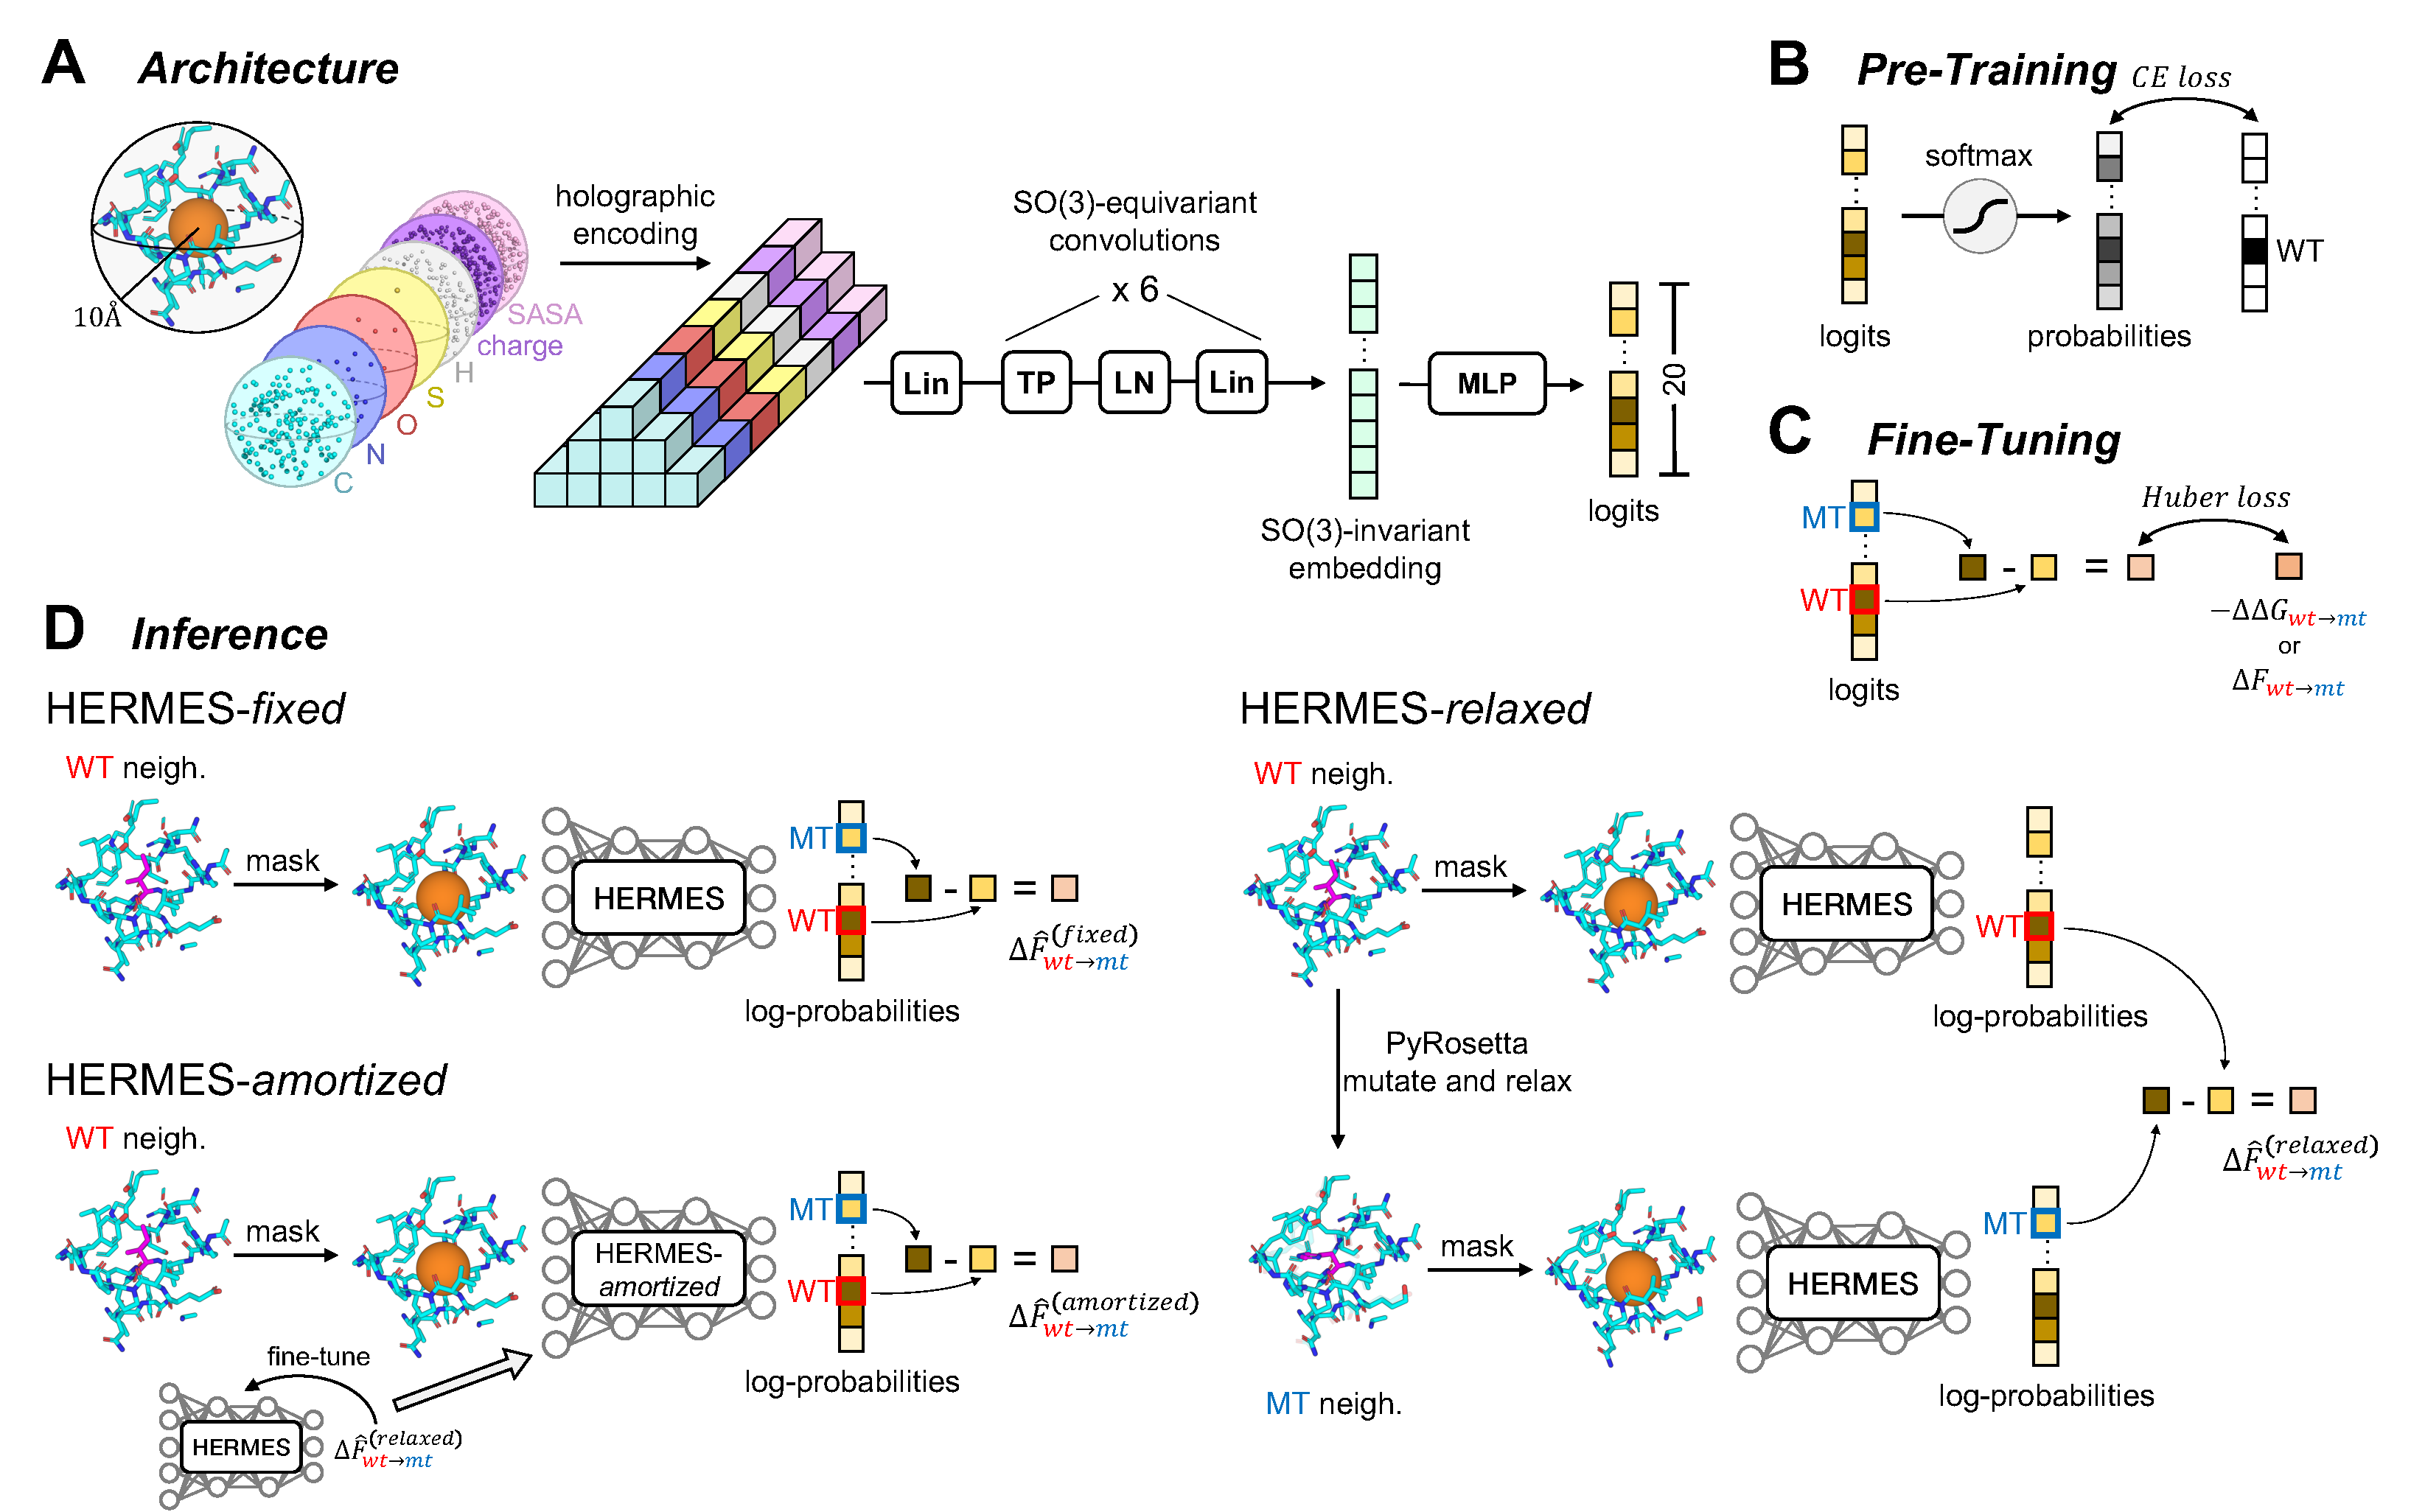
\includegraphics[width=1.0\linewidth]{figures/hermes_with_inference.pdf} \figcaption{Overview of
    HERMES.}{
    \textbf{(A)} Model architecture: HERMES takes as input an all-atom structural neighborhood
    (10~\AA{} radius) around a masked focal residue. Each atom is represented by its 3D coordinates,
    element type, partial charge, and solvent-accessible surface area (SASA). The neighborhood is
    projected onto a Zernike Fourier basis (spherical hologram) and processed by {rotation (SO(3))}
    equivariant layers to produce a rotation-invariant embedding, which is mapped to 20
    amino-acid-specific logits (Methods).\textbf{(B)}
    Pre-training: models are trained to predict the identity of the masked focal residue from its
    surrounding {atomic} neighborhood; logits in (A) are converted to amino-acid propensities
    (probabilities) via a softmax. \textbf{(C)}
    Fine-tuning for mutational effects: model weights are optimized to regress the logit difference
    between mutant and wild-type amino acids to the {corresponding} experimental mutational effect.
    \textbf{(D)} Inference protocols. HERMES-{\em fixed} scores a substitution as the difference
    between the the mutant and wild-type amino-acids logits from a single forward pass, conditioned
    on the masked wild-type neighborhood $X_\wt$. HERMES-{\em relaxed} conditions the mutant term on
    an approximate mutant neighborhood $\hat X_{\wt\to\mt}$ generated in-silico by introducing the
    mutation on the wild-type structure and locally relaxing the structure {with}
    Rosetta~\citep{chaudhury_pyrosetta_2010}. {HERMES-{\em amortized}} distills the relaxed protocol
    by fine-tuning on HERMES-{\em relaxed} predictions, enabling fast fixed-style inference while
    retaining relaxation-aware behavior.}
    \label{fig:HERMES}
\end{figure}


\section{Methods}

\noindent{\bf HERMES architecture and pre-training on masked amino acid classification.}

At its core, HERMES is a 3D, rotationally equivariant convolutional neural network that predicts the propensity
of the 20 different canonical amino acids at a masked (removed) {focal} residue, given its local
atomic neighborhood within the protein structure (Fig.~\ref{fig:HERMES}A).

Atomic neighborhoods - centered at the focal residue's C$\alpha$ and with radius 10~\AA~- are 
first featurized by atom type (including added hydrogens), partial charge,
and solvent-accessible surface area, and then encoded into \textit{holograms} via the ZFT
(Eq.~\ref{eq:ZFT}). Then, a stack of SO(3)-equivariant layers - shown in Fig.~\ref{fig:HERMES}A and detailed
in Section~\ref{sec:layers} - map this encoding to a
rotation-invariant embedding, which a final MLP converts into amino-acid propensities.

For pre-training, we train HERMES to recover the identity of the masked residues on ProteinNet's
CASP12 set, filtered at 30\% sequence identity~\citep{alquraishi_proteinnet_2019}
(Fig.~\ref{fig:HERMES}B). Each model is an ensemble of 10 independently trained networks (3.5M
parameters each), with predictions averaged at inference. To improve robustness for zero-shot
applications, we additionally train models with 0.50~\AA~coordinate noise. Pre-training performance
is summarized in Table~\ref{table:aa_wt_cls}. See Extended Methods in Appendix~\ref{sec:hermes_appendix}
for further details.


\noindent{\bf Zero-shot prediction of mutational effects with pre-trained HERMES.}
The pre-trained HERMES model outputs $P(aa| X_{i,aa})$, the probability of assigning amino acid $aa$
at residue $i$, given the surrounding atomic environment (neighborhood) $X_{i,aa}$ in the structure.
Crucially, $X_{i,aa}$ depends on the $aa$: the neighborhood geometry has the fingerprint of the
masked amino acid during pre-training.

Conditional models are widely used for zero-shot prediction of mutational effects on protein
function (e.g., \citep{riesselman_deep_2018, meier_language_2021, pun_learning_2024}). We
approximate the effect of wild-type to mutant ($\wt \to \mt$) substitution at residue $i$ by the
log-likelihood ratio between the wild-type and the mutant amino acids, conditioned on the respective
local atomic neighborhoods $X_{i,\wt}$ and $X_{i,\mt}$ (omitting the residue index $i$ for clarity):
\begin{equation}
\begin{aligned}
  \Delta \hat F_{\wt \to \mt}  \propto  \log P(\mt | X_{\mt}) - \log P(\wt | X_{\wt})
\end{aligned}
\label{eq:log_ratio_wt_and_mt}
\end{equation}
Here, the neighborhood $X$ depends on the identity of the original amino acid ($\wt$ or $\mt$),
suggesting the potential need for having access to mutant structures for such predictions. The
$\hat\cdot$ {(hat)} indicates the model-predicted mutational effects, as opposed to experimental
measurements (no hat).

When a mutant structure is unavailable, neighborhoods can be relaxed {\em in silico} (e.g., by
Rosetta~ \citep{chaudhury_pyrosetta_2010}), though this procedure is computationally expensive. A
common alternative is to score all mutations using a single (typically wild-type)
structure~\citep{dauparas_robust_2022,diaz_stability_2024,pun_learning_2024}. Here, we {consider}
both of these protocols: {\bf HERMES-{\em fixed}} evaluates mutational effects using the wild-type
structure only (for both $\mt$ and $\wt$ propensities), while {\bf HERMES-{\em relaxed}} evaluates
the propensity of the mutant amino acid in the Rosetta-relaxed $\mt$ neighborhood $\hat X_{\wt \to
\mt}$ starting from the available $\wt$ structure (Fig.~\ref{fig:HERMES}D); see Methods for details.
The resulting estimates for mutational effects from these two approaches follow,
\begin{equation}
\begin{aligned}
\Delta \hat F_{\wt \to \mt}^{\text{(HERMES-{\em fixed})}} &\propto \log P\left(\mt \mid
X_{\wt}\right) - \log P\left(\wt \mid X_{\wt}\right)\\
\Delta \hat F_{\wt \to \mt}^{\text{(HERMES-{\em relaxed})}} &\propto \log P\left(\mt \mid \hat
X_{\wt \to \mt}\right) - \log P\left(\wt \mid X_{\wt}\right).
\end{aligned}
\label{eq:deltaF_variants}
\end{equation}

\noindent{\bf Fine-tuning HERMES to predict protein function.}
Context-conditioned amino-acid likelihoods provide useful zero-shot proxies for mutational effects
across diverse functions~\citep{riesselman_deep_2018, meier_language_2021, pun_learning_2024}, but
supervised models for specific functions can perform better in practice. Building on prior
work~\citep{blaabjerg_rapid_2023, diaz_stability_2024}, we fine-tune HERMES models directly on
mutational effect data. Unlike approaches that train a separate regression
head~\citep{blaabjerg_rapid_2023, diaz_stability_2024, dieckhaus_transfer_2024}, we update the
model end-to-end so that its \emph{predicted scores} themselves align with measurements.
Specifically, as shown in Fig.~\ref{fig:HERMES}C,
we make the predicted HERMES-{\em fixed} $\Delta \hat F_{\wt \to \mt}^{\text{(HERMES-{\em fixed})}}$
(eq.~\ref{eq:deltaF_variants}) regress over the experimentally measured mutational effects $\Delta
F_{\wt\to \mt}$ by minimizing a robust Huber loss,
\begin{equation}
   \mathcal{L} = \text{HuberLoss}(\Delta \hat F_{\wt \to \mt}^{\text{(HERMES-{\em fixed})}}, \Delta
   F_{\wt \to \mt})
\label{eq:loss_function}
\end{equation}
which stabilizes training under outliers while calibrating predictions to the function of interest.
See Extended Methods in Appendix~\ref{sec:hermes_appendix} for further details.\\


\noindent{\bf Hermes-{\em amortized} to encode structural flexibility in HERMES-{\em fixed} by
amortization.}
Because the structural-relaxation step in HERMES-\emph{relaxed} is computationally costly ($\sim 66$
times slower than HERMES-{\em fixed} on a single CPU / A40 GPU, Table~\ref{table:inference_speed}),
we distill HERMES-\emph{relaxed} predictions into the model via a fine-tuning procedure. Concretely,
we fine-tune the model so that the mutational-effect predictions produced with the fast
HERMES-\emph{fixed} protocol regress to the corresponding HERMES-\emph{relaxed} predictions {via
Eq.~\ref{eq:loss_function}} (Fig.~\ref{fig:HERMES}D). We perform this fine-tuning on a small subset
of neighborhoods extracted from the pre-training proteins ($\sim$15k neighborhoods, 0.5\% of the
total). The resulting amortized model HERMES-{\em amortized} runs at HERMES-\emph{fixed} speed
(effectively the same protocol, just different model weights) yet closely matches
HERMES-\emph{relaxed} performance (Fig.~\ref{fig:relaxed_vs_ft_relaxed}).\\



\section{Results}

\subsection{Predicting mutational effects on thermodynamic fold-stability}
\label{sec:results_stability}

The chief task we evaluated the HERMES models on was to predict mutational effects on thermodynamic
folding stability.
Thermodynamic folding stability is defined as the change in Gibbs Free $\Delta G$ energy upon
folding. Thus, the effect of a mutation $\wt \rightarrow \mt$ on folding stability is denoted by
$\Delta \Delta G_{\wt \rightarrow \mt} = \Delta G_\mt - \Delta G_\wt$.\\
\begin{figure}[ht!]
    \centering
    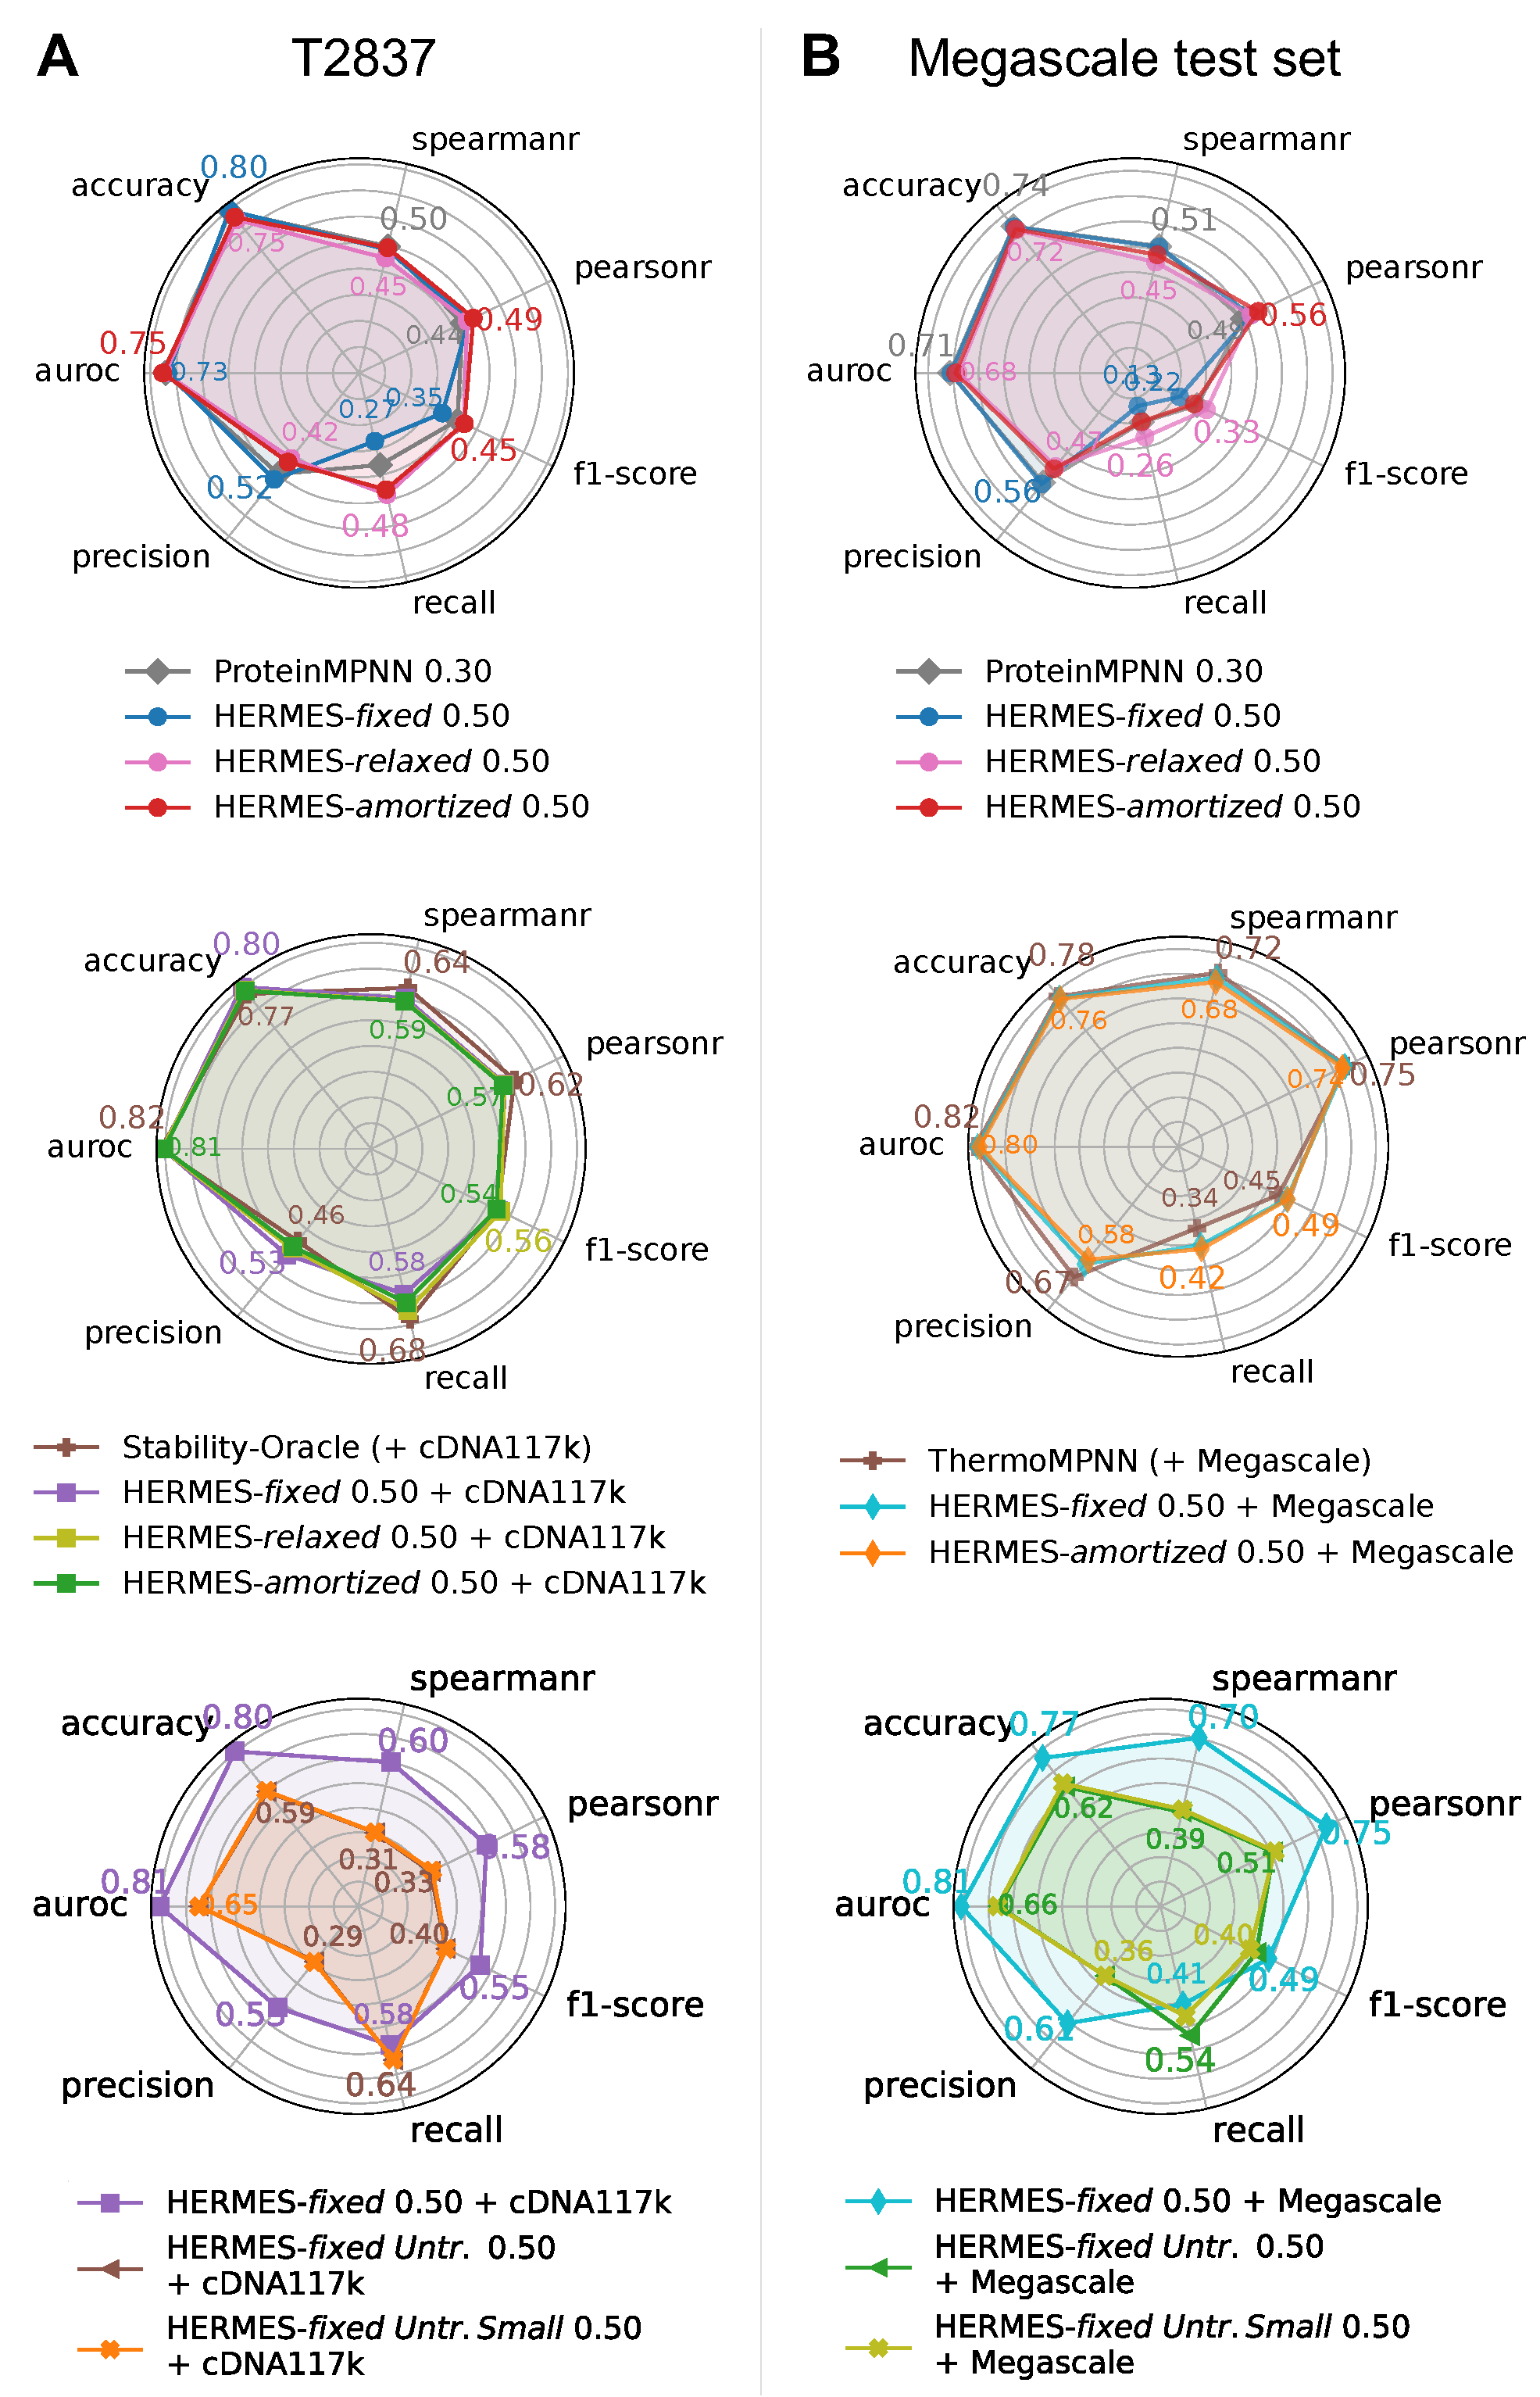
\includegraphics[width=0.70\textwidth]{figures/radial_plots__noise__no_numbers.pdf}
    \figcaption{Predicting mutational effects on thermodynamic folding stability.}{
    Stabilizing-versus-destabilizing classification metrics are computed using $\Delta\Delta G < 0$
    (experimental) and $\Delta \log p > 0$ (predicted) as cutoffs for stabilizing mutations.
    \textbf{(A)} T2837 results: zero-shot models (top) and models fine-tuned or only trained on
    cDNA117k (middle and bottom). \textbf{(B)} Megascale test set results: zero-shot models (top)
    and models fine-tuned or only trained on the Megascale training set (middle and bottom). Model
    names indicate the architecture, the coordinate-noise amplitude used, and when applicable, the
    fine-tuning dataset (listed after ``$+$"); \textit{Untr.} is short for \textit{Untrained},
    indicating models that had no pre-training and were instead only trained on stability effects.
    Only models trained with coordinate noise are shown; the noise amplitude is indicated within
    each model name {as standard deviation in~\AA~units}. Results for models trained without noise
    are provided in Fig.~\ref{fig:radial_plots__no_noise}.
    }
   \label{fig:radial_plots__noise}
\end{figure}

\noindent {\bf Training and test Data.} To enable a direct comparison with recent structure-based
stability predictors, we fine-tuned and evaluated HERMES on the same benchmark splits used by
RaSP~\citep{blaabjerg_rapid_2023}, Stability-Oracle~\citep{diaz_stability_2024}, and
ThermoMPNN~\citep{dieckhaus_transfer_2024}. Specifically, we (i) trained on the RaSP Rosetta-derived
stability dataset and tested on the experimental benchmark used in RaSP, (ii) used
Stability-Oracle's curated cDNA117k training set and T2837 test set; training on 117k $\Delta\Delta
G$ values from ref.~\citep{tsuboyama_mega-scale_2023} filtered by enforcing $\leq 30\%$ sequence
identity to the test set, and (iii) trained on ThermoMPNN's Megascale \textit{train} split and
evaluated on its Megascale \textit{test} split, both from ref.~\citep{tsuboyama_mega-scale_2023};
training on 216k and testing on 28k mutation effects with 25\% sequence-identity cutoff. Because
these splits are defined by the original studies, our results are directly comparable across
methods. We additionally note that the Megascale \textit{train} split is not de-duplicated against
T2837, and six of the T2837 proteins ($\sim 5\%$) have $>90\%$ sequence-similar homologs in the
Megascale training set; see Methods for more details on these training and test sets.\\



\noindent\textbf{Noise and side-chain relaxation improve zero-shot model predictions.} We first
evaluated the \emph{zero-shot} HERMES models (no fine-tuning on experimental data) on the T2837 and
Megascale test sets (Fig.~\ref{fig:radial_plots__noise}, \ref{fig:radial_plots__no_noise}).
Pre-training on structures with Gaussian coordinate noise (0.5~\AA{} s.d.) improves performance,
consistent with prior work~\citep{dauparas_robust_2022, pun_learning_2024}. Relative to
HERMES-\emph{fixed}, the packing-aware HERMES-\emph{relaxed} achieves significantly higher recall
(0.48 vs. 0.27; p-value $<$ 0.01), with only a slight loss in precision, leading to a higher overall
F1-score. HERMES-\emph{amortized} performs similarly to HERMES-\emph{relaxed}: on T2837, and on
Megascale, it shows slightly lower recall and F1 while still outperforming HERMES-\emph{fixed}; the
p-values for the significance of these performance differences are reported in
Fig.~\ref{fig:t2837_and_megascale_pairwise_pvalues_permutation}.

To test whether packing awareness preferentially improves predictions for substitutions that perturb
local packing, we stratified mutations by residue size. Wild-type and mutant residues were assigned
to small, medium, or large classes using normalized van der Waals volumes~\citep{mei_new_2005}, and
we evaluated stabilizing-versus-destabilizing classification performance within each $\wt \to \mt$
size-transition group (Fig.~\ref{fig:megascale_precision_recall_f1_by_size_cutoff_0p0}).


Switching from HERMES-{\em fixed} to HERMES-{\em relaxed} yielded the largest recall gains in
identifying stabilizing substitutions between residues with substantially different sizes. This
improvement was most pronounced for large$\to$small substitutions: HERMES-{\em fixed} is constrained
by the rigid wild-type cavity, preventing it from recognizing that mutations that create voids could
be stabilizing, whereas HERMES-{\em relaxed} can repack neighbors to fill the space and stabilize
the smaller side chain. While precision changes varied across size categories, F1-score improved in
all categories, with the largest gains occurring for small$\to$large substitutions, where relaxation
can reorganize the local environment to accommodate bulkier side chains that would otherwise clash.
Interestingly, HERMES-\emph{amortized}, which learned packing implicitly through fine-tuning, showed
comparable improvements for large$\to$small substitutions but much weaker gains for small$\to$large
substitutions. This could suggest that stabilizing small$\to$large substitutions may be
underrepresented in the fine-tuning training set; the p-values associated with the significance of
performance differences between models within each size-transition category, and within models
across different size-transition categories are reported in
Figs.~\ref{fig:pvalues__bucketed_by_size__between_small_large_buckets__vertical},~\ref{fig:t2837_and_megascale_pairwise_pvalues_permutation}.

For comparison, we evaluated ProteinMPNN~\citep{dauparas_robust_2022}
on the same tasks. ProteinMPNN outperformed HERMES-{\em fixed}, and performed on par with
HERMES-\emph{relaxed} on both small$\to$large and large$\to$small mutations
(Fig.~\ref{fig:megascale_precision_recall_f1_by_size_cutoff_0p0},~\ref{fig:pairwise_pvalues_permutation_bucketed_by_sizereduced_precision_recall_f1}).
We attribute this performance to ProteinMPNN's input representation: by conditioning only on
backbone coordinates and residue identities, ProteinMPNN is less constrained by the explicit
wild-type side-chain geometry compared to the all-atom HERMES-{\em fixed} model. This architectural
choice enables implicit reasoning about side-chain flexibility, achieving results comparable to
using explicit relaxations in HERMES-{\em relaxed}. Notably, ProteinMPNN performed better than
HERMES-{\em amortized} on small$\to$large substitutions.\\



\begin{figure}
    \centering
    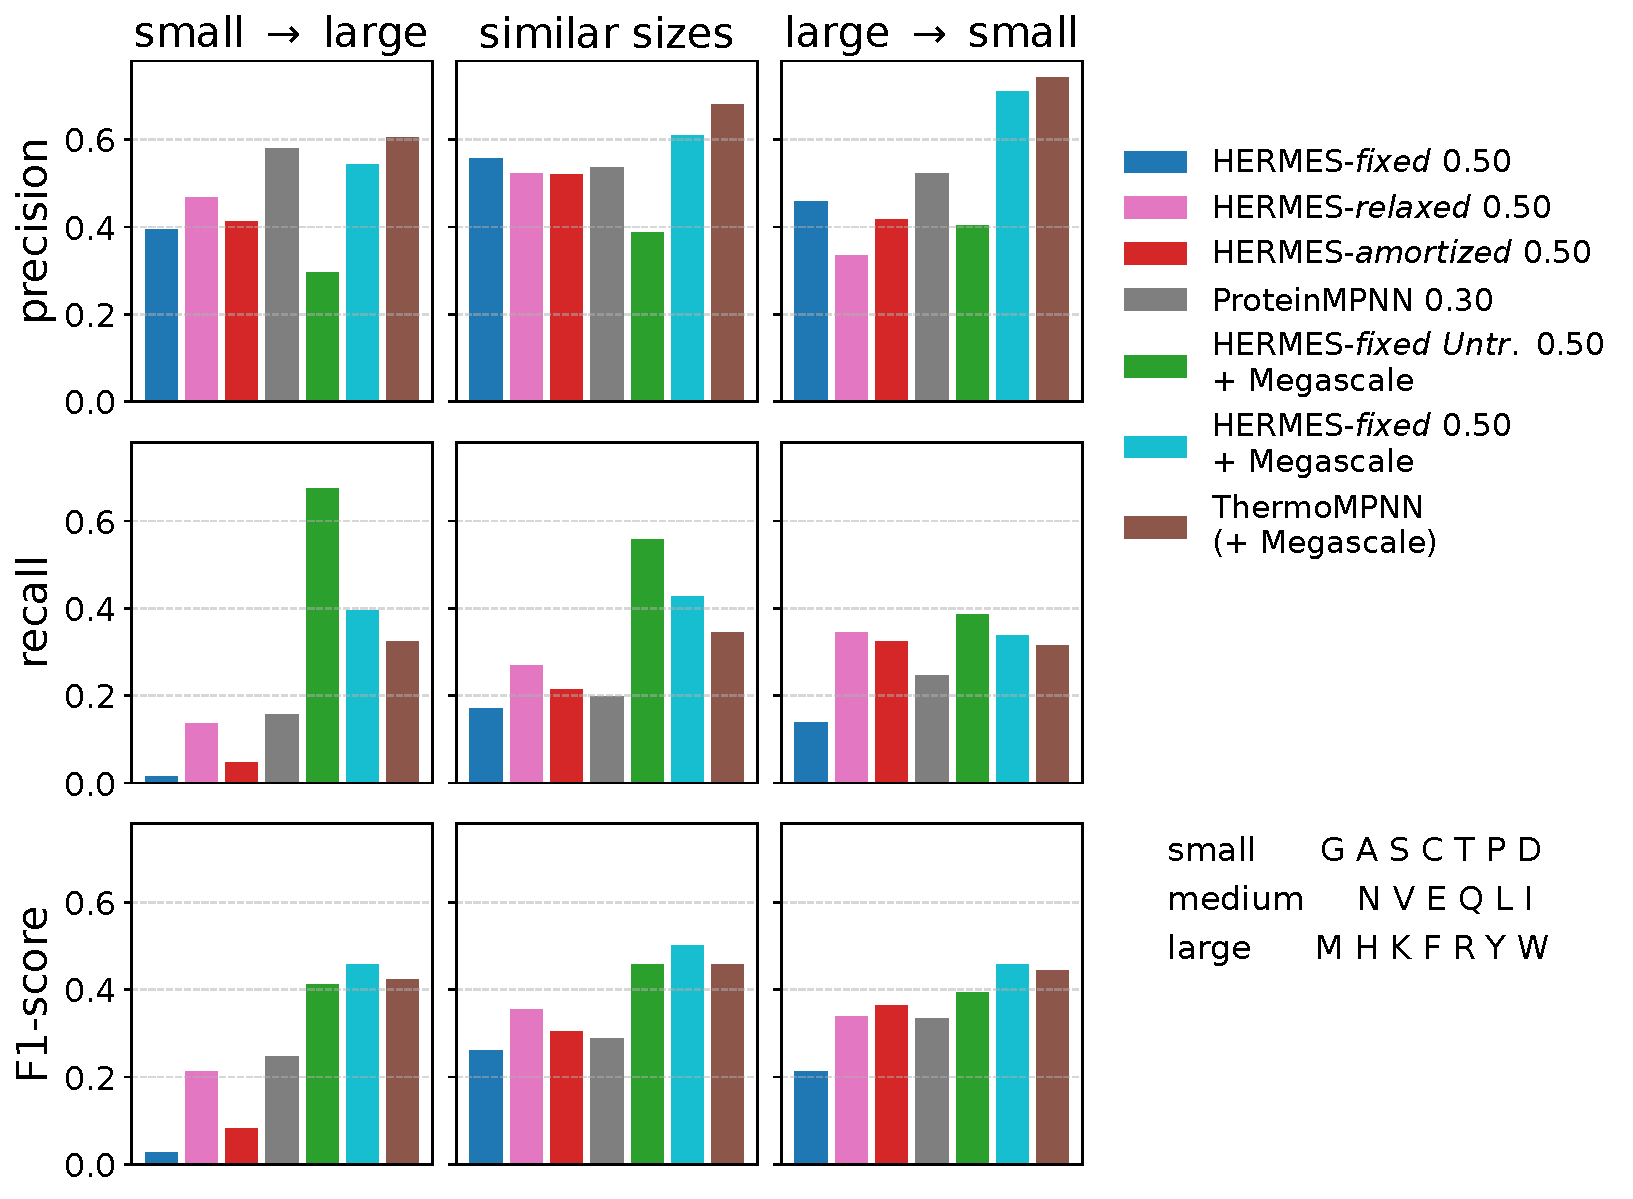
\includegraphics[width=0.9\textwidth]{figures/barplots_bucketed_by_size__zeroshot_plus_finetuned__precision_and_recall_and_f1.pdf}
    \figcaption{Impact of amino acid size changes on predicting mutational effects on protein
    stability.}{
    Amino acids are grouped into three size classes based on van der Waals volume (as listed), and
    predictions are stratified by wild-type and mutant size classes; ``similar sizes" denote
    substitutions within the same class.
    Stabilizing-versus-destabilizing classification metrics (rows) are then computed and shown for
    each stratum (columns), using $\Delta\Delta G < 0$ (experimental) and $\Delta \log p > 0$
    (predicted) as cutoffs for stabilizing mutations.
    P-values for pairwise model comparisons are shown in
    Fig.~\ref{fig:pairwise_pvalues_permutation_bucketed_by_sizereduced_precision_recall_f1}, and
    p-values comparing each model's performance on small$\to$large vs. large$\to$small substitutions
    are shown in Fig.~\ref{fig:pvalues__bucketed_by_size__between_small_large_buckets__vertical}.
    Model names indicate the architecture, the coordinate-noise amplitude used during pre-training
    {as standard deviation in~\AA~units}, and when applicable, the fine-tuning dataset (listed after
    ``$+$").
}    \label{fig:megascale_precision_recall_f1_by_size_cutoff_0p0}
\end{figure}
\noindent {\bf Fine-tuned HERMES models achieve state-of-the-art performance for stability effect
prediction.}
When fine-tuning on the respective stability effect datasets, HERMES outperformed RaSP
(Fig.~\ref{fig:rasp_exp}), and matched the performance of Stability-Oracle
(Fig.~\ref{fig:radial_plots__noise}A,~\ref{fig:t2837_broken_down_and_comparison}) and ThermoMPNN
(Fig.~\ref{fig:radial_plots__noise}B).
These results underscore both the effectiveness of the HERMES architecture and the importance of
fine-tuning data for test-time accuracy. HERMES was also robust to using ESMFold-resolved
structures~\citep{lin_evolutionary-scale_2023} for either fine-tuning or inference
(Fig.~\ref{fig:radial_plots__esmfold}), supporting practical use cases where only computationally
predicted structures are available.

Removing pre-training on wild-type amino-acid classification significantly degraded performance:
HERMES models trained {\em only} for stability prediction performed poorly when trained on either
cDNA117k or Megascale, even after reducing capacity from 3.5M parameters to 50k to mitigate
overfitting (Fig.~\ref{fig:radial_plots__no_noise}). A similar failure mode was reported for
ThermoMPNN on the Megascale training data~\citep{dieckhaus_transfer_2024}.

Finally, fine-tuning on stability effects largely eliminated size-dependent bias, yielding
comparable recall and F1 scores for small$\to$large and large$\to$small substitutions
(Figs.~\ref{fig:megascale_precision_recall_f1_by_size_cutoff_0p0},~\ref{fig:pvalues__bucketed_by_size__between_small_large_buckets__vertical}).\\


\begin{figure}
    \centering
    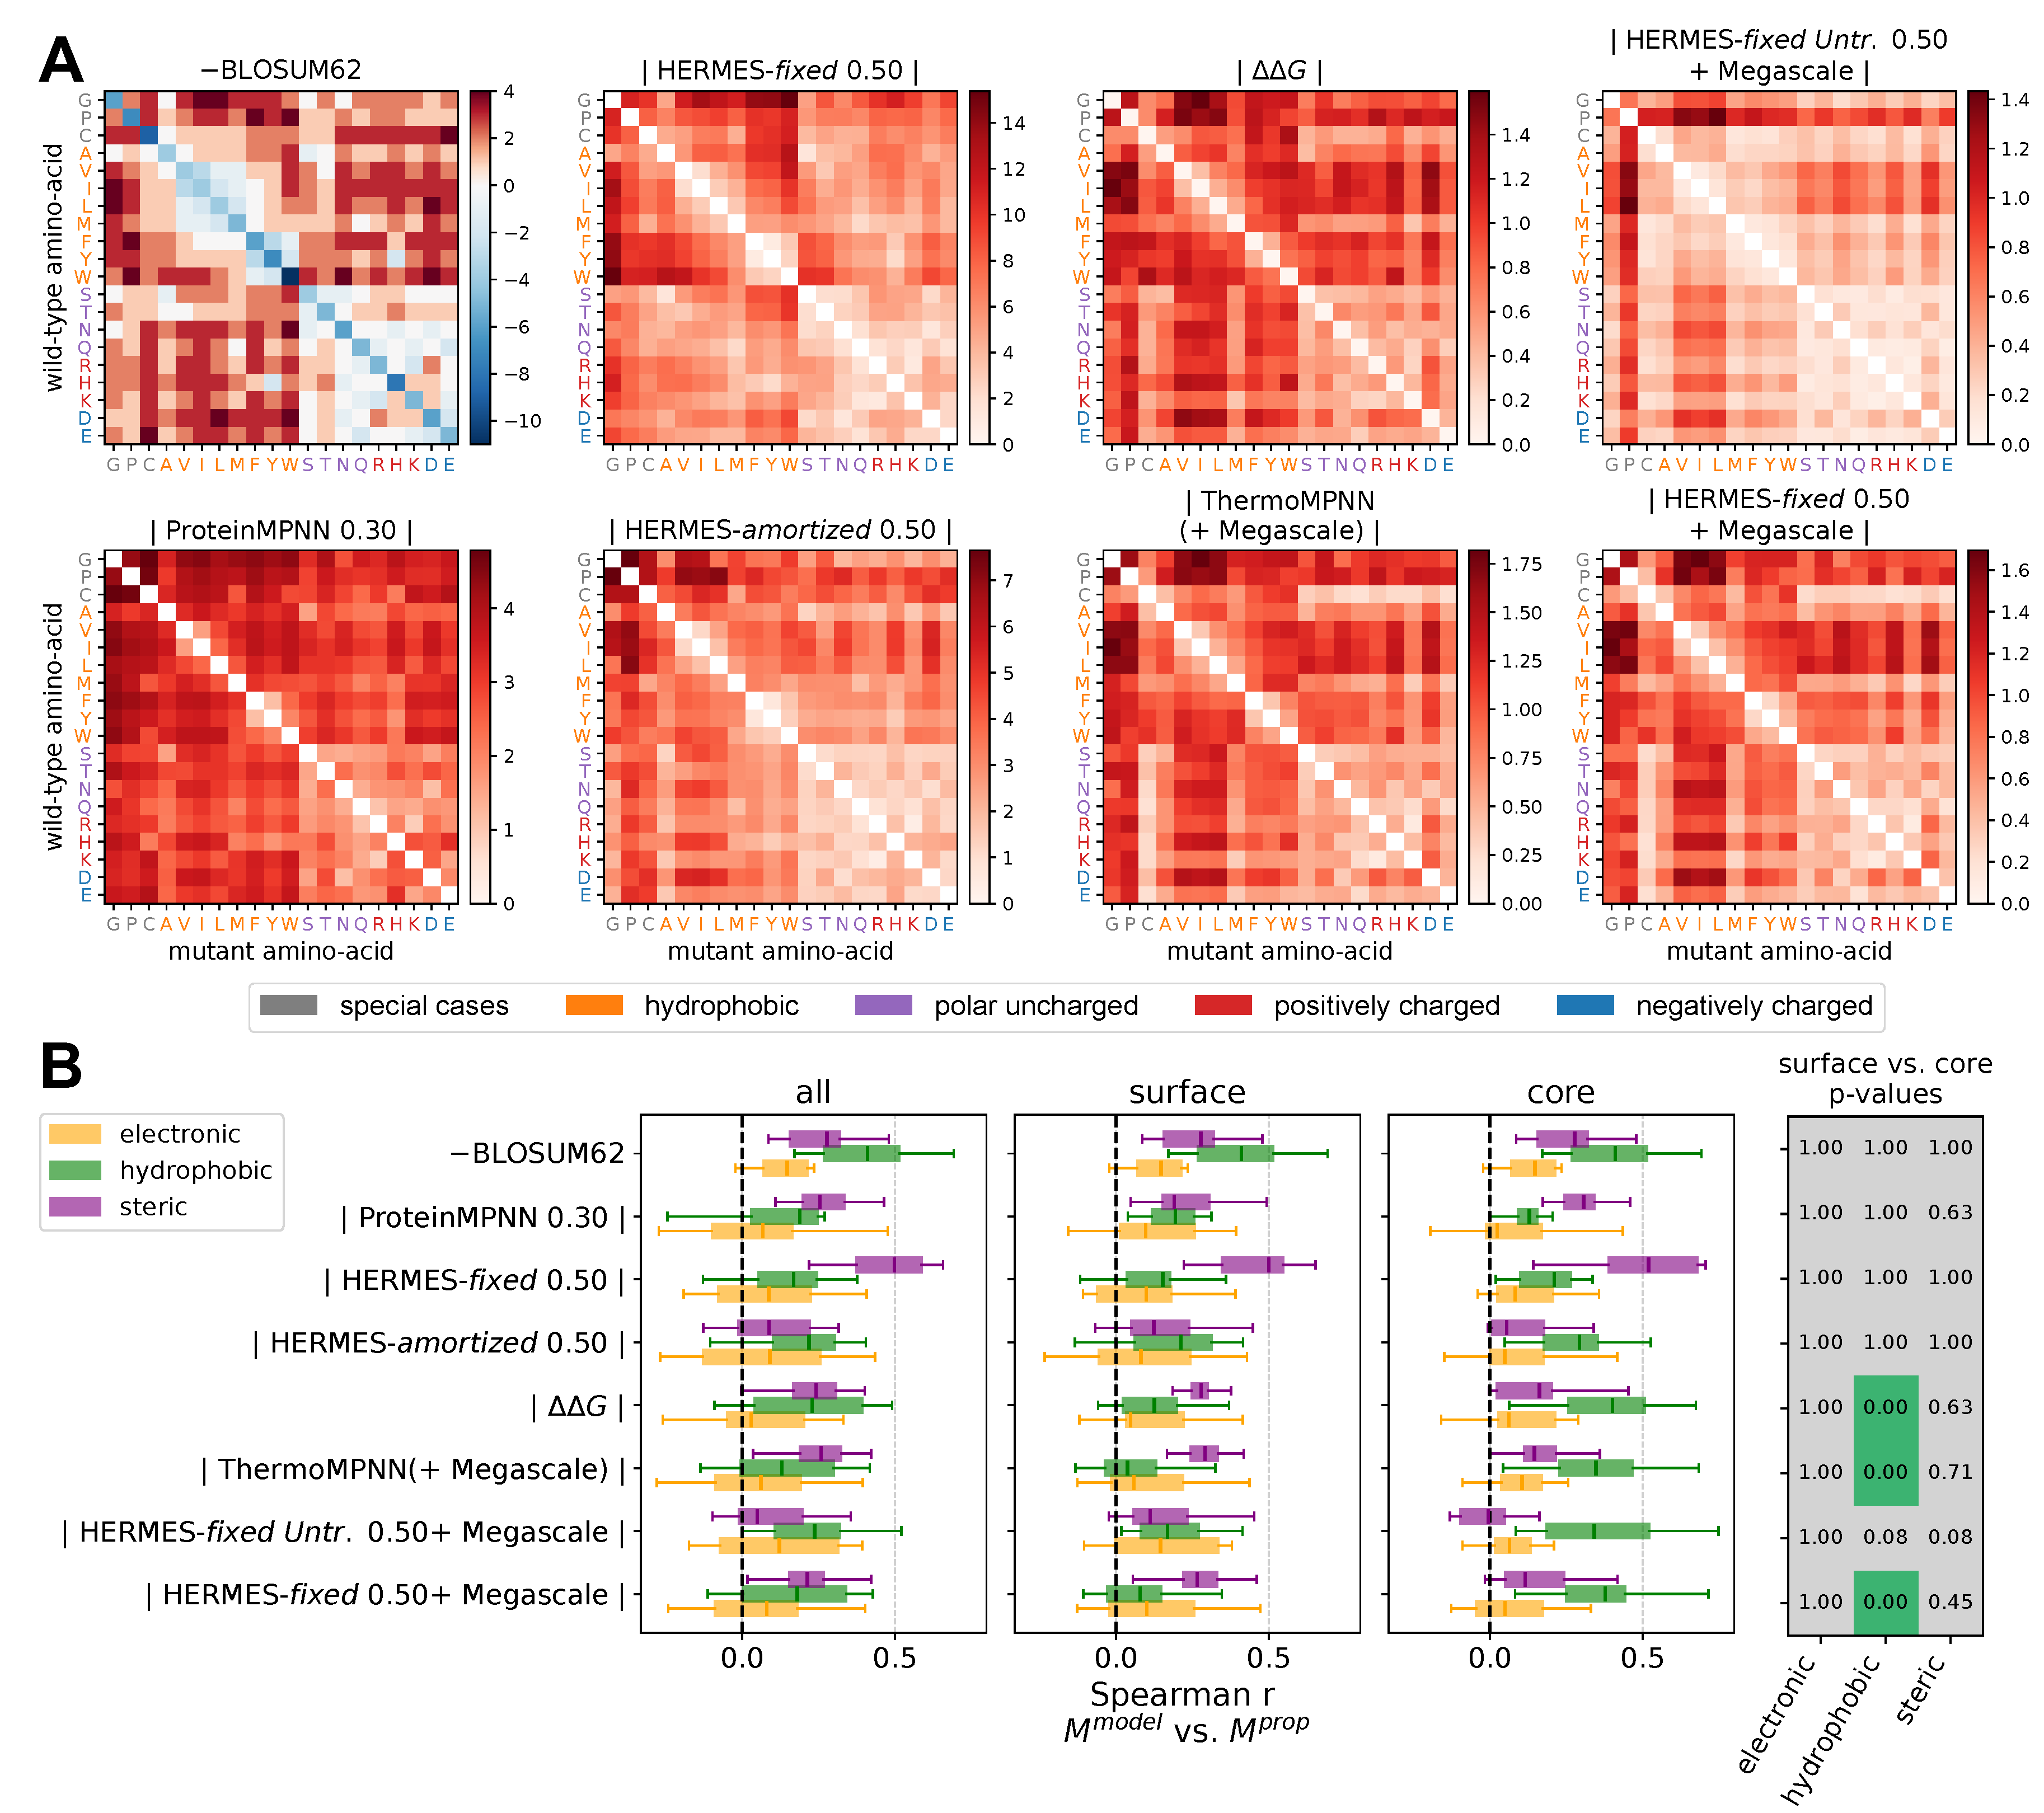
\includegraphics[width=1.0\textwidth]{figures/confusion_matrices_and_boxplot_with_abs.pdf}
    \figcaption{Uncovering mutation preferences via model-averaged substitution matrices.}{
    \textbf{(A)} 
    Heatmaps of model-averaged substitution matrices $M^{\model}$ computed by averaging over the
    Megascale test set, shown alongside BLOSUM62 and and the experimental matrix of mean
    $|\Delta\Delta G|$ values across mutations.
    Spearman correlations between matrices are reported in
    Fig.~\ref{fig:spearmanr_between_model_average_substitution_matrices}. Core- and
    surface-restricted matrices (core: SASA $< 1 \AA^2$; surface: SASA $> 3 \AA^2$) are shown in
    Fig.~\ref{fig:average_prediction_matrices__abs_symm__part_1}~and~\ref{fig:average_prediction_matrices__abs_symm__part_2}.
    \textbf{(B)} For each model and site subset (all, surface, core), boxplots summarize Spearman
    correlations between $M^{\model}$ and property-difference matrices $M^{\prop}$, grouped by
    property class (color). P-values from two-tailed t-tests comparing the surface vs. core
    correlations within each property class are shown on the right. P-values for between-model
    comparisons of property-class correlations are shown in
    Fig.~\ref{fig:correlation_to_aa_properties__significance}.
      }
    \label{fig:correlations_to_aa_properties}
\end{figure}

\noindent \textbf{Biophysical interpretation of HERMES predictions for mutational stability
effects.}
We sought to quantify how much models' mutation preferences could be explained by amino-acid
physicochemical properties. Specifically, we asked which properties are shared by amino-acid pairs
that the model treats as interchangeable, i.e., substitutions with $\Delta \hat{F} \approx 0$ on
average.

To do this, we constructed model-averaged substitution matrices $M^{\model}$ whose $(\alpha,\beta)$
entry represents how neutrally the model treats exchanging amino acids $\alpha$ and $\beta$. For
each pair $(\alpha,\beta)$, we computed the model-predicted mean {\em absolute} effect,
$M^{\model}_{\alpha, \beta} = \langle |\Delta \hat{F}^{(\model)}_{\alpha,\beta} |\rangle$, where
$\langle \cdot \rangle$
denotes averages over all $\alpha\to \beta$ and $\beta\to \alpha$ substitutions in the Megascale
test set. This procedure yields a symmetric, non-negative $20\times 20$ matrix for each model, in
which values approaching zero indicate greater predicted interchangeability. For comparison, we
constructed an analogous matrix using experimentally measured $|\Delta\Delta G|$ values from the
Megascale test set ($M^{|\Delta\Delta G|}$), and include the BLOSUM62 substitution matrix as an
additional reference.

Following ref.~\cite{pyo_data-driven_2025}, we also constructed symmetric, nonnegative matrices of
\emph{absolute amino-acid property differences}. Specifically, we considered 50 quantitative
properties spanning (i) hydrophobic, (ii) electronic, and (iii) steric categories
(Table~\ref{table:aa_properties}), yielding 50 property-specific matrices $M^{\prop}$ with the
$(\alpha,\beta)$ entry: $M^{\prop}_{\alpha,\beta} = |\prop_\alpha - \prop_\beta|$. Smaller values
indicate greater similarity between the two amino acids with respect to the specified property.


To quantify which biophysical properties each model tends to preserve, we computed the Spearman
correlation between the model-averaged substitution matrix
 $M^{\model}$ and each of property-specific amino acid distance matrix $M^{\prop}$
 (Fig.~\ref{fig:correlations_to_aa_properties}B).
Consistent with the size-stratified analysis
(Fig.~\ref{fig:megascale_precision_recall_f1_by_size_cutoff_0p0}), HERMES-{\em fixed} predicted
amino-acid interchangeability align most strongly with steric properties, particularly average
buried-residue volume (Spearman $r =0.66$) and normalized van der Waals volume (Spearman $r =
0.64$). This correlations was significantly stronger than for the other models (p-values in
Fig.~\ref{fig:correlation_to_aa_properties__significance}).
In contrast, BLOSUM62, derived from evolutionary substitution frequencies, preferentially preserves
hydrophobic properties. When restricting $M^{\model}$ to core residues (SASA $< 1$\AA$^2$), the
interchangeability matrix associated with stability-fine tuned models {(e.g.
$M^{\text{HERMES-\textit{fixed} 0.50 + Megascale}}$)} showed stronger alignment with hydrophobic
properties, to levels comparable to BLOSUM62 and consistent with the experimental matrix
$M^{|\Delta\Delta G|}$.
Zero-shot models instead did not show a comparable increase in hydrophobic preservation when
restricting to the core (Fig.~\ref{fig:correlations_to_aa_properties}B).\\




\begin{figure}[ht!]
    \centering
    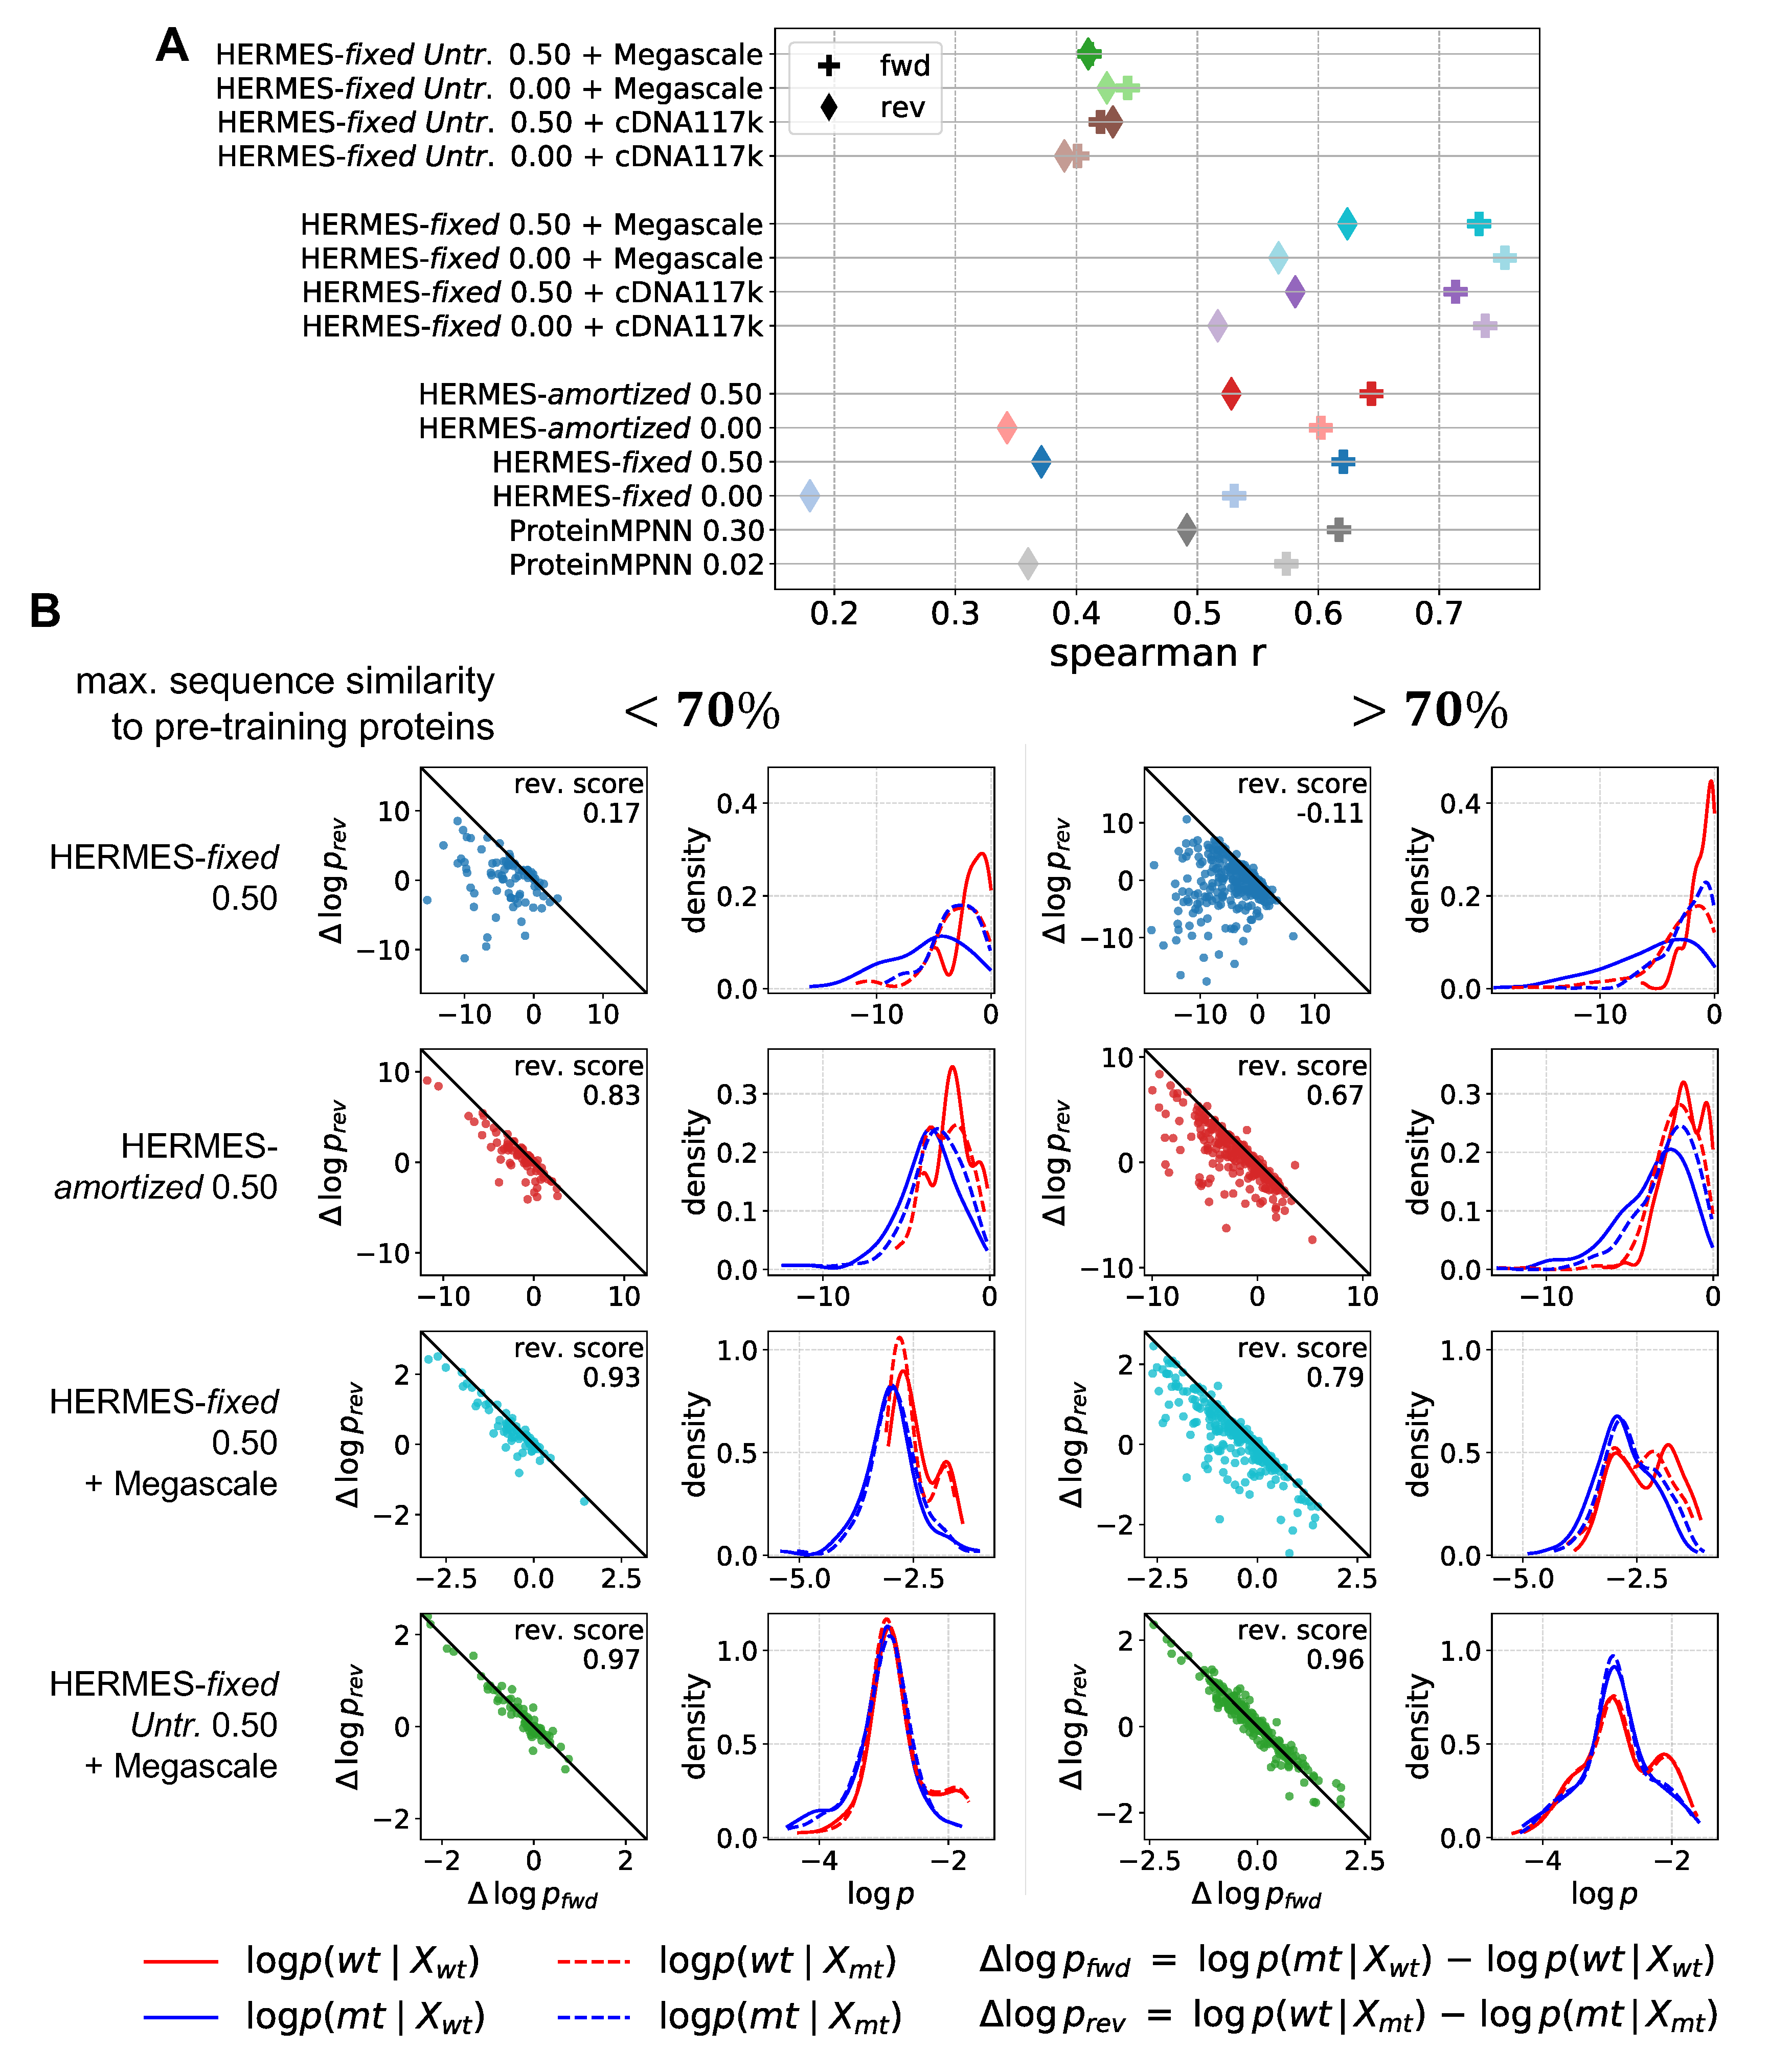
\includegraphics[width=0.9\textwidth]{figures/reversibility_and_wt_bias.pdf}
    \figcaption{Identifying model biases with structure-conditioned reversibility}{
    \textbf{(A)} 
   Spearman correlations between experimental stability changes ($\Delta\Delta G$ and model
   predictions on the Ssym dataset are shown. For each model, we report correlations for forward
   substitutions ($\Delta \log p_{fwd}$ vs. $\Delta\Delta G$) and the reverse substitutions ($\Delta
   \log p_{rev}$ vs. $-\Delta\Delta G$). {\bf(B)} Ssym proteins are stratified by their maximum
   sequence identity to pre-training proteins ($\geq 70\%$ vs. $< 70\%$). For each split (columns)
   and four representative HERMES variants (rows), the left panel shows the scatter plots for
   $\Delta \log p_{fwd}$ vs. $\Delta \log p_{rev}$; an unbiased model should exhibit strong
   anti-correlation, summarized by the reversibility score (rev.; higher is more reversible;
   Eq.~\ref{eq:rev_score}). Reversibility is highest for the model not pre-trained on wild-type
   amino-acid classification (green; bottom row) and is consistently higher for the low-similarity
   subset. Fig.~\ref{fig:ssym_antisymmetry_reversibility_score_results} shows the reversibility
   scores across all models in (A). In each column, the right panel shows the distributions of the
   log-probabilities that make up $\Delta \log\,p_{fwd} = \log p (\mt | X_\wt) - \log p (\wt|X_\wt)$
   (solid lines) and $\Delta \log\,p_{rev} = \log p (\wt | X_\mt) - \log p (\mt|X_\wt)$ (dashed
   lines). All models except for the one that was \textit{not} pre-trained on wild-type amino-acid
   classification (last row) exhibit elevated $\log p(\wt\,|X_{\wt})$.
    }
    \label{fig:ssym_figure}
\end{figure}
   
\noindent{\bf Reversibility and path-independence of HERMES predictions with respect to mutations.}
Mutational effects are, in principle, reversible: the effect of substituting a residue from amino
acid $\alpha$ to $\beta$ should be equal in magnitude and opposite in sign to the reverse change,
i.e., $\Delta F_{\alpha \to \beta} = -\Delta F_{\beta\to \alpha}$. Moreover, equilibrium quantities
such as protein stability free energy are state functions. As such, the net effect of a multi-step
substitution depends only on the initial and final amino acids, not on the mutational path. For a
path $\alpha \to \beta \to \gamma$, this implies: $\Delta F_{\alpha\to \gamma} = \Delta F_{\alpha\to
\beta} + \Delta F_{\beta\to \gamma}$.



HERMES predicts mutation effects as differences in amino-acid-specific log-probabilities (logits)
$\log p(aa | X_{aa})$ (both zero-shot and after fine-tuning). As log-probability differences under a
fixed structural context, these predictions satisfy reversibility by construction:
\EQ 
\Delta \hat F^{(\text{model})}_{\alpha\to \beta} = \log P(\beta | X_{\beta}) - \log P(\alpha
|X_{\alpha}) = -\Delta \hat F^{(\text{model})}_{\beta\to \alpha}
\label{eq:reversibility}
\EE
where we set $X_{\alpha}= X_{\beta}$ for HERMES-{\em fixed} and HERMES-{\em amortized}, and
$X_{\beta}= \hat X_{\alpha\to \beta}$ for HERMES-{\em relaxed}. Path-independence follows similarly.
In contrast, other structural models such as Stability-Oracle~\citep{diaz_stability_2024} require
explicit $19\times$ data augmentation (termed ``thermodynamic permutation augmentation" in
ref.~\citep{diaz_stability_2024}) to enforce these properties.

Alternatively, reversibility can be assessed in a structure-conditioned
manner~\citep{blaabjerg_rapid_2023, dieckhaus_transfer_2024}, where the effects of forward
$\alpha\to \beta$ and reverse $\beta \to \alpha$ substitutions are computed using the outgoing
structural contexts, i.e., $\alpha\to \beta$ is conditioned on $X_{\alpha}$ and $\beta\to\alpha$ on
$X_{\beta}$ (Extended Methods, Appendix~\ref{sec:hermes_appendix}). Under this transformation, we do
not automatically expect a
``structure-conditioned reversibility", as forward and reverse transitions are conditioned on
different structures. However, a well-balanced model should have near-reversibility in this setting,
making this a stringent test of model bias. We measured structure-conditioned reversibility on the
Ssym dataset, which contains wild-type and single-mutant structures for 352 mutations across 19
proteins~\citep{pancotti_predicting_2022}.
For each mutation, we computed a ``forward" effect ($\wt \to\mt$, conditioned on the wild-type
structure) and a ``reverse" effect ($\mt \to\wt$, conditioned on the mutant structure).


We found that zero-shot HERMES models and ProteinMPNN predict stability effects more accurately for
forward substitutions ($\wt \to\mt$) than for the reverse direction, consistent with previous
observations~\citep{blaabjerg_rapid_2023, dieckhaus_transfer_2024} (Fig.~\ref{fig:ssym_figure}A).
Adding coordinate noise during pre-training and fine-tuning on stability effects both reduced this
forward-reverse disparity, but did not eliminate it. Models trained {\em only} on stability effects
showed little or no disparity, albeit with substantially lower overall accuracy.
Across all pre-trained models, the predicted stability effects of forward mutations from the
wild-type tend to have larger magnitudes than those of the corresponding reverse mutations
(Fig.~\ref{fig:ssym_figure}B, scatterplots). This bias stems from the elevated log-probabilities
assigned to wild-type amino acids in wild-type structure neighborhoods $\log p(\wt | X_{\wt})$
(Fig.~\ref{fig:ssym_figure}B, density plots), suggesting a wild-type preference that may reflect
pre-training memorization. Consistently, stratifying Ssym proteins by sequence similarity to the
pre-training set (Extended Methods, Appendix~\ref{sec:hermes_appendix}) yielded a modest reduction
in wild-type preference for lower-similarity
proteins (Fig.~\ref{fig:ssym_figure}B). A more detailed characterization of this bias is left to
future work.

\begin{figure}[t!]
    \centering
    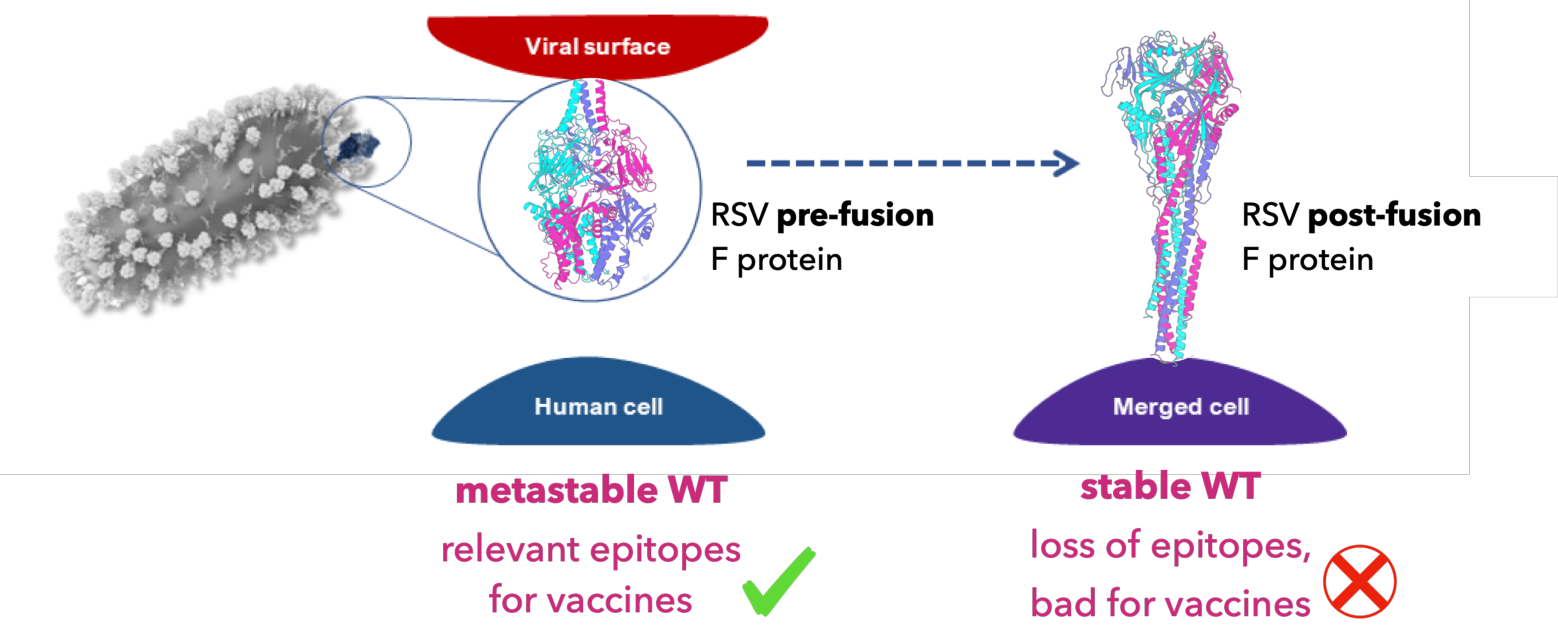
\includegraphics[width=0.9\linewidth]{figures/antigen_design_concept.pdf}
    \figcaption{\GM{Overview of structure-based vaccine design against enveloped viruses.}}{
        \GM{
            A large proportion of viruses are enveloped by a bi-lipid membrane akin to that of human cells,
            The infect human cells, they make use of specialized proteins that latch onto the cell's
            membrane and ``fuse" it to the virus' envelope. This fusion process is enabled by a
            conformational change in the fusion protein: from a ``pre-fusion" to a ``post-fusion"
            conformation.
            Naturally, vaccines should be engineered to elicit immune responses that target epitopes
            presented \textit{before} the virus has infected the cell, i.e. while the fusion protein
            is in the pre-fusion conformation.
            However, the wild-type of fusion viruses is generally more stable in the post-fusion
            conformation.
            Therefore, the field of structure-based vaccine design has proposed to use vaccines
            containing engineered mutants of the fusion proteins that are more stable in
            pre-fusion relative to post-fusion.
            Figure adapted from \url{https://www.niaid.nih.gov/diseases-conditions/safe-and-effective-rsv-protein-vaccines}.
        }
    }
    \label{fig:antigen_design_concept}
\end{figure}


\subsection{Antigen stabilization with HERMES for vaccine design}
Structure-based vaccine design seeks to increase vaccine efficacy by \GM{engineering viral envelope
glycoproteins (hereafter, ``antigens") to be more stable in their pre-fusion conformation,
relative to their post-fusion conformation (Figure~\ref{fig:antigen_design_concept}).
Pre-fusion stabilization} enriches presentation of neutralization-relevant epitopes and can bias elicited immune responses
toward protective specificities.
\GM{In the literature, it is achieved by applying a minimal set of mutations to the fusion protein that either improve the stability
of the pre-fusion conformation, or decrease that of the post-fusion conformation, while preserving the relevant
epitopes~\citep{mclellan_structure-based_2013, gonzalez_general_2024, bakkers_efficacious_2024, milder_universal_2022, phan_conserved_2022}.

Practitioners often classify mutations in different types
based on the manner in which they provide relative pre-fusion stabilization (hereafter, ``antigen stabilization").
For example, {\em Cavity-filling mutations} mutations stabilize the pre-fusion conformation by filling cavities
located within the hydrophobic core, by inserting a larger hydrophobic side-chain.
{\em Proline mutations} instead are often used to impede post-fusion $\alpha$-helix formation and
stabilize pre-fusion conformations, due to proline's unique lack of amide hydrogens which prevents
it from taking part in stable $\alpha$-helices.
Other mutation types include {\em electrostatic mutations}, which introduce polar or charged amino acids in environments
where they can engage in stabilizing electrostatic interactions,
and finally {\em synergistic mutations}, which involve applying multiple mutations so that they positively interact
through a variety of mechanisms.
We show examples of mutation types in Fig.~\ref{fig:antigen_figure_of_different_types_of_mutations}A.
}

\GM{
The use of computational tools to guide antigen stabilization has precedents in the literature,
but it is largely limited to the use of scoring functions like Rosetta~\citep{gonzalez_general_2024, phan_conserved_2022},
with few closed-source attempts to use machine learning~\citep{bakkers_efficacious_2024}.
Therefore, we sought out to test whether HERMES can be used to aid vaccine design campaigns.

Unfortunately, large scale datasets of experimentally-validated mutations are not yet present.
Thus, we started the campaign by manually collecting 33 previously reported antigen-stabilizing mutations drawn from
five viral antigens: Influenza HA~\citep{milder_universal_2022} (3 mutations),
RSV-F~\citep{mclellan_structure-based_2013, lee_rational_2024} (7 mutations),
hMPV-F~\citep{gonzalez_general_2024, bakkers_efficacious_2024, phan_conserved_2022} (11 mutations),
DENV-E~\citep{phan_conserved_2022} (8 mutations), and SARS-CoV-2 spike
protein~\citep{hsieh_structure-based_2020} (4 mutations).
We then benchmarked model performance on their ability to identify the specific mutants
as the most pre-fusion-stabilizing within their respective sites; essentially evaluating per-site recall.
We scored mutations using zero-shot and
stability-fine-tuned variants of ProteinMPNN and HERMES. Importantly, none of the stabilized
variants in this benchmark appeared in the training data of any HERMES model, either during
pre-training or during stability fine-tuning.
}

\begin{figure}[t!]
    \centering
    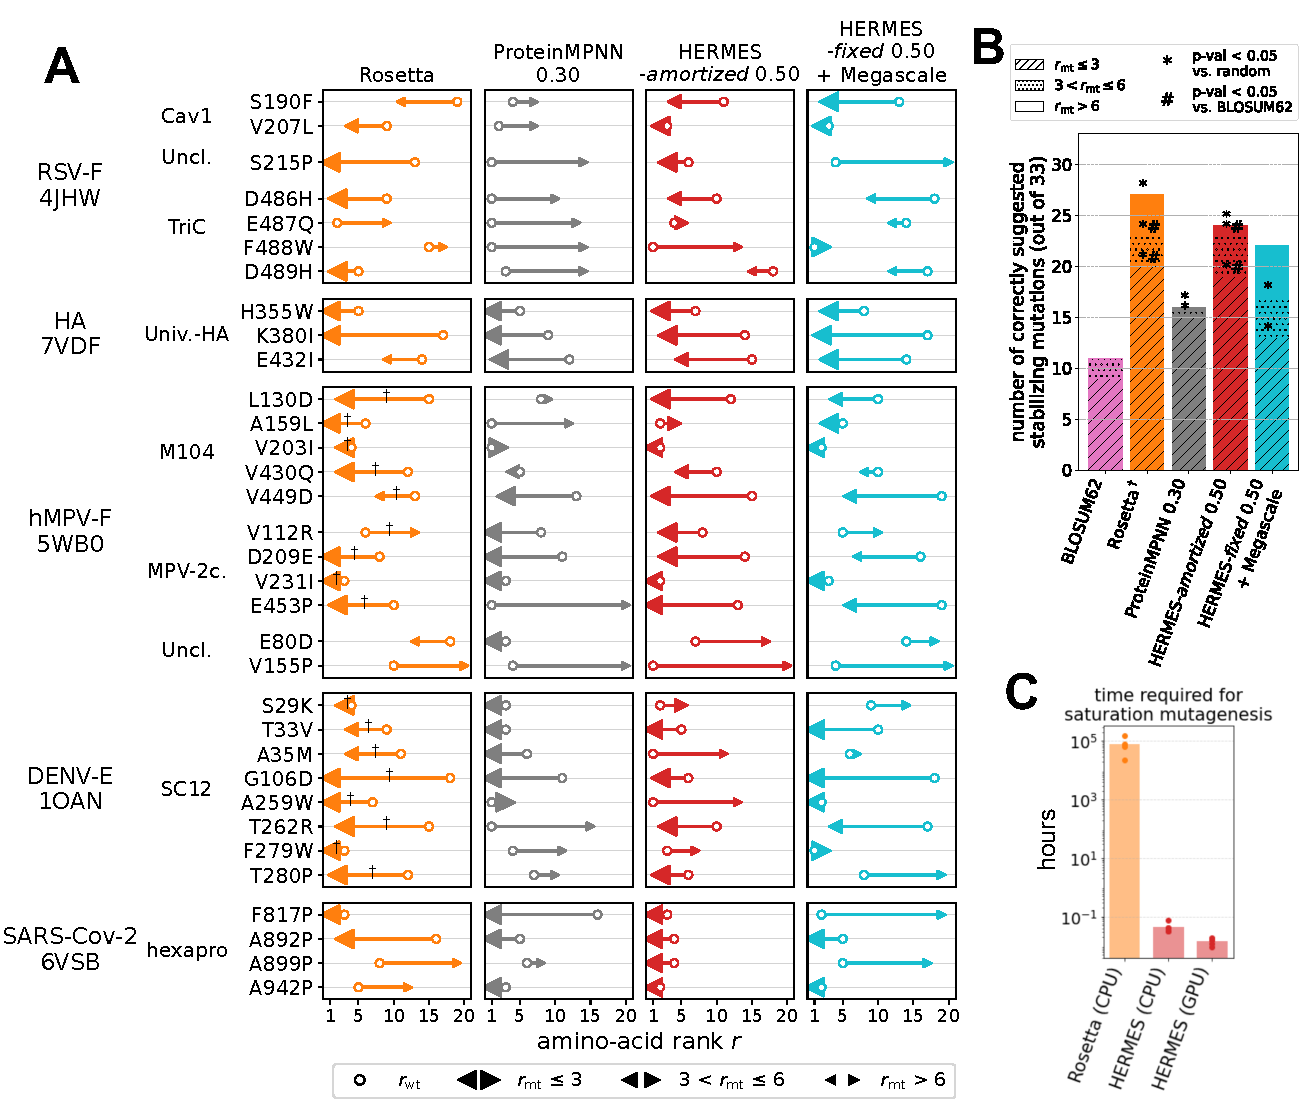
\includegraphics[width=1.0\linewidth]{figures/antigen_figure_main_results_with_time.pdf}
    \figcaption{Recovering previously-identified antigen-stabilizing mutations with HERMES.}{
    \textbf{(A)} Model recall is evaluated on 33 previously reported antigen-stabilizing mutations
    (rows) across five viral antigens. For each antigen, the PDB structure used for scoring is
    indicated. Mutations are specified as wild-type$\to$mutant substitutions at the annotated site.
    Four models (columns) are compared, as labeled above each column; see
    Table~\ref{table:antigen_results} for a more extensive comparison of models on this task. Arrows
    depict the change in predicted rank from the wild type (open circle) to the stabilizing mutant
    (arrow tip); arrow size indicates whether the mutant ranks in the top 3 (large), ranks 4--6
    (medium), or ranks $>6$ (small). The $\dagger$ symbols mark mutations originally proposed as
    stabilizing by Rosetta. ``Univ.-HA" stands for ``Universal-HA"; ``MPV-2c." stands for
    MPV-2cREKR; ``Uncl." stands for ``Uncleaved Prefusion-Closed".
    {\bf (B)} Counts of correctly
    prioritized antigen-stabilizing mutations ($r_\mt < r_\wt$), stratified by predicted rank group:
    strongly suggested ($r_\mt \leq 3$), moderately suggested ($3 < r_\mt \leq 6$), or weakly
    suggested ($6\leq r_\mt$) are shown for each model. For comparison, BLOSUM62 is used to rank
    substitutions into the ($r_\mt \leq 3$) or ($3 < r_\mt \leq 6$) groups; under this scheme the
    wild-type residue is always ranked first. Statistical enrichment is assessed by comparing the
    number of strong/moderate recalls to a random-ranking baseline and to BLOSUM62 (denoted by ($*$)
    and ($\#$), respectively, when binomial tests corrected p-value$<0.05$; see Methods).
    We note that all structures were considered in their native multimeric state, generating
    symmetric partners with PyMOL when necessary.
    \GM{{\bf (C)} Estimated times for saturation mutagenesis predictions on the viral antigens considered
    in this study. Each dot is an antigen. Times shown are for a single CPU and a single NVIDIA A40 GPU.
    See Table~\ref{table:speed_on_antigens} for precise per-antigen times.}
    }
    \label{fig:antigen_figure_main_results}
\end{figure}
 
To quantify performance, we emulated a simple model-guided selection workflow in which a
practitioner considers substitutions at a site in descending order of model scores. For each known
stabilizing mutation, we record its rank $r_\mt$ among all 20 amino acids at that position and
compare it to the wild-type rank $r_\wt$. We posit that a practitioner would select a particular
mutant for experimental validation if (1) its rank $r_\mt$ is better (lower) than that of the
wild-type $r_\wt$, and (2) its rank is among the top-scoring candidates (lower end). We categorize
each predicted-stabilizing mutation (i.e., with $r_\mt < r_\wt$) as strongly suggested ($r_\mt \leq
3$), moderately suggested ($3 < r_\mt \leq 6$), or weakly suggested ($r_\mt > 6$)
(Fig.~\ref{fig:antigen_figure_main_results} {and Table~\ref{table:antigen_results}}). This scheme
would group mutations with similar physico-chemical properties into the same rank class.
Consequently, models are generally not penalized for ranking a biophysically similar alternative
above a known stabilizing mutant, making our performance metrics robust to fine-grained rank
differences in different models (see Fig.~\ref{fig:antigen_heatmap} and Appendix~\ref{sec:hermes_appendix}
for a more detail discussion on antigen-stabilizing mutations).

Figs.~\ref{fig:antigen_figure_main_results},~\ref{fig:antigen_figure_of_different_types_of_mutations}
{and Table~\ref{table:antigen_results}} summarize predictions across the 33 stabilizing mutations we
studied. Among the machine-learning methods, HERMES-\emph{amortized} performs best: it assigns a
better (lower) rank than wild-type to 24 stabilizing mutations, including 19 classified as strongly
suggested ($r_\mt \leq 3$). Notably, stability fine-tuning does not consistently improve performance
over the corresponding zero-shot ProteinMPNN and HERMES-{\em amortized} on this task
(Table~\ref{table:antigen_results}).

For comparison, we also scored each mutant with Rosetta~\citep{chaudhury_pyrosetta_2010},
(Extended Methods, Appendix~\ref{sec:hermes_appendix}).
Rosetta recovers stabilizing mutations on par with HERMES-\emph{amortized}
({Fig.~\ref{fig:antigen_figure_main_results} and} Table~\ref{table:antigen_results}); however, 17
variants in this benchmark were originally selected (by the references that discovered the variants)
using Rosetta-based screening, which partially biases this baseline in Rosetta's favor.
Most importantly, however,
Rosetta inference is substantially more computationally intensive than the machine learning models,
limiting its practicality for predicting the stability effects in high-throughput saturation
mutagenesis \GM{(Fig.~\ref{fig:antigen_figure_main_results}C)}.

To assess statistical enrichment of model predictions over chance, we compared the predicted number
of stabilizing mutations in the strong/moderate categories to a random-ranking baseline using a
binomial test (Extended Methods, Appendix~\ref{sec:hermes_appendix}); p-values are reported in
Fig.~\ref{fig:antigen_pvalues_vs_random}. All models except for HERMES-{\em fixed} and ThermoMPNN
significantly outperform random ranking in
recovering stabilizing mutations with strong or moderate confidence
({Table~\ref{table:antigen_results}}).
As an additional baseline, we tested whether the BLOSUM62 (B62) substitution matrix can prioritize
stabilizing mutations. BLOSUM62 recovers significantly fewer stabilizing mutations in the
strong/moderate categories than HERMES-\emph{amortized} (defined as $r_\mt^{B62} \leq 3$ and
$r_\mt^{B62} \leq 6$, noting that $r_\wt^{B62} = 1$ always; {results shown in
Fig.~\ref{fig:antigen_figure_main_results},} and binomial test p-values reported in
Fig.~\ref{fig:antigen_pvalues_vs_blosum62}), underscoring the value of incorporating structural
context when predicting stabilizing substitutions.

\GM{For a more detailed analysis, we manually annotated the 33 antigen-stabilizing mutations based on their mutation types
(Table~\ref{table:mutation_types}) and accordingly stratified model performance (Fig.~\ref{fig:antigen_figure_of_different_types_of_mutations}B).}
Among the models tested, HERMES-\emph{amortized} most reliably recovers stabilizing proline
mutations (7 out of 8; Fig.~\ref{fig:antigen_figure_of_different_types_of_mutations}B), highlighting
its potential utility for proposing pre-fusion stabilizing prolines. More broadly, all models
recover proline and electrostatic mutations at higher rates than expected under BLOSUM62, whereas
cavity-filling mutations show weaker gains. A plausible explanation is that cavity-filling changes
typically replace a smaller hydrophobic residue with a larger one that preserves core
hydrophobicity. Because such substitutions are common in natural sequence variation, they are partly
captured by a sequence-derived matrix like BLOSUM62. In contrast, proline and charged substitutions
are strongly context-dependent, with effects that hinge on local geometry and environment, and
therefore benefit more from structure-aware modeling; see Appendix~\ref{sec:hermes_appendix} for a more detailed discussion.

Lastly, the synergistic RSV-F TriC mutations are difficult to recover for almost all methods
(Fig.~\ref{fig:antigen_figure_main_results}). This is expected for the three ``acid patch
neutralization" substitutions D486H, D489H, and E487Q~\citep{mclellan_structure-based_2013}, which
were experimentally stabilizing only in combination (i.e., synergy) with
F488W~\citep{mclellan_structure-based_2013}. These four residues are tightly clustered in both
intra- and inter-chain space, consistent with a synergistic (epistatic) mechanism in which the
substitutions act synergistically to stabilize the trimer. A second example of synergy is the DENV-E
pair A259W and T262R, which together introduce a favorable cation-$\pi$ interaction
(Fig.~\ref{fig:antigen_figure_of_different_types_of_mutations}A.4). Because our evaluation scheme
scores mutations in a site-independent manner, the models are not able to capture such multi-residue
dependencies. Specifically, HERMES scores mutations at a single site under the assumption that all
other amino-acid identities remain fixed, and therefore, cannot recover stabilization mechanisms
that arise only from specific combinations of mutations. ProteinMPNN, ThermoMPNN, and Rosetta are
likewise evaluated here under the same site-independent protocol for a fair comparison, although
they can in principle be applied to score multi-residue variants jointly; see Appendix~\ref{sec:hermes_appendix} for a more
detailed discussion.

Beyond the inability to capture epistatic effects, several additional limitations of our approach
should be noted. First, to emulate a practitioner's workflow we evaluate mutations using only their
relative ranks; however, the absolute magnitudes of model scores carry additional information and
could enable more robust decision-making when prioritizing antigen-stabilizing mutations. Second,
because the original studies rarely tested comprehensive alternative substitutions at the same
sites, we cannot evaluate the models' ability to propose different stabilizing mutations that were
not assayed experimentally. Third, experimental validation frequently involved multi-mutation
constructs, complicating attribution of observed stabilization to any single residue. Finally, the
modest number of curated stabilizing mutations limits statistical power and the strength of
conclusions in our analyses. Despite these caveats, our results suggest that HERMES can serve as a
practical screening tool for rational library design, prioritizing candidate antigen-stabilizing
mutations for more efficient experimental validations.

\GM{
While the above analysis uses experimentally-verified antigen stabilizing mutations as ground truth,
it is limited by a low sample size, and the fact that it measures only per-site recall.
Therefore, it is not fully indicative of performance during a design campaing, in which precision is also a key metric.

Despite a lack of extensive experimental ground truth, we sought to demonstrate the practical utility
of HERMES by designing a workflow for suggesting individual antigen-stabilizing mutations.
We considered two pipelines for suggesting mutations with HERMES.\\
{\em 1) Stabilize pre-fusion core:} the first and simplest pipeline focuses on suggesting mutations that stabilize the pre-fusion conformation,
ignoring possible effects to the post-fusion conformation.
Specifically, given an pre-fusion structure, we scored all possible mutations all sites in the core (average SASA $< 1 \text{\AA}^2$),
via $\Delta \log p^{pre-f}$, where higher scores indicate higher predicted stabilized effects.
We then sorted the mutations by score, and considered as suggestions the top 80 mutations, with a limit
of maximum 3 mutations at the same site to encourage more site variability; crucially, all mutations are predicted
to be stibilizing by HERMES ($\Delta \log p^{pre-f} > 0$).\\
{\em 2) Stabilize pre-fusion and destabilize post-fusion:} for the second pipeline instead we aim to suggest mutations that both stabilize the pre-fusion conformation,
and destabilize the post-fusion conformation. Specifically, we consider as suggestions the top 80 mutations (again, max 3 per site)
sorted by $\Delta \log p^{pre-f} - \Delta \log p^{post-f}$, and subject to both $\Delta \log p^{pre-f} > 0$
and $\Delta \log p^{post-f} < 0$. For this approach, we do not pose any constraints on site locations.

Of the HERMES models, we only considered HERMES-{\em amortized} as it was the best performing model in the ground truth recall analysis.
For baselines, we considered mutations sampled with ProteinMPNN, BLOSUM62, and at random.
Specifically, for ProteinMPNN we selected 80 mutations per pipeline in the same exact manner as with HERMES.
For BLOSUM62 we randomly selected 80 sites per pipeline (either in pre-fusion core only or unrestrictedly),
and took the top two mutations by BLOSUM62 score.
Finally, we sampled 160 mutations at random (max 3 per site, either in pre-fusion core only or unrestrictedly). 
For all models and pipelines, we excluded mutations to and from cysteine residues, both to avoid breaking disulfide bonds,
and in consideration of the fact that stabilizing cysteine mutations usually come in pairs precisely to form
disulfide bonds.

Due to the lack of experimental ground truth, we resort to using Rosetta as an oracle.
Rosetta scores are computed analogously to the previous analysis (Figure~\ref{fig:antigen_figure_main_results}),
but with higher sample size.
Specifically, for each mutation, the full structure with both wild-type and mutant amino-acid is
relaxed and scored 50 times, yielding a distribution of 50 scores in Rosetta Energy Units (REU).
These are then summarized into a single composite score ($S_{ros}$) by averaging the best (lowest) 20\% of the values.
Then, a suggested mutation is considered a ``Rosetta hit" if either
$\Delta\,S_{ros}^{pre-f} > 0$, or both $\Delta\,S_{ros}^{pre-f} > 0$ and $\Delta\,S_{ros}^{post-f} < 0$,
respectively following the analogous pipeline used for suggesting mutations.

Using Rosetta as oracle implies a model's performance should be interpreted as how much it agrees with Rosetta, not explicitly with experiments.
However, we still consider this a useful exercise.
Indeed, Rosetta's ability to identify stabilizing mutations is validated by our recall analysis~\ref{fig:antigen_figure_main_results},
and by previous studies with experimental validation~\citep{gonzalez_general_2024, phan_conserved_2022}.
Despite this, Rosetta is very slow (Figure~\ref{fig:antigen_figure_main_results}C), prohibitively so if CPU resources are limited.
Thus, first using a fast model - like HERMES - to rank all possible mutations such that top mutations are agreed upon by
Rosetta can accelerate the finding of truly antigen-stabilizing mutations.
Furthermore, using the consensus of multiple models to generate candidates with the highest likelihood of experimental success
is a ubiquitous strategy in protein design~\citep{butcher_novo_2025, abramson_accurate_2024},
and adopted in this thesis also in Chapter~\ref{sec:tcrpmhc}.

We ran both design pipelines on the RSV-F and DENV-E proteins, reporting respective results in Figures~\ref{fig:rsv_f_rosetta_hits_main_figure}
~and~\ref{fig:denv_e_rosetta_hits_main_figure}.
HERMES-{\em amortized} consistently outperforms - in terms of Rosetta hits - all baselines, with the exception of ProteinMPNN
in the ``stabilize pre-fusion and destabilize post-fusion" pipeline.
The greatest alignment with Rosetta is observed in the ``stabilize pre-fusion core" pipeline, where 7 of the top 10 mutations
are validated by Rosetta, compared to 4 by ProteinMPNN and 2 if picked at random (Figure~\ref{fig:rsv_f_rosetta_hits_main_figure}).
Plotting the amino-acid pairs involved in successfully suggested mutations, reveals that HERMES can identify cavity-filling
mutations in the core (small hydrophobic $\to$ large hydrophobic and polar $\to$ hydrophobic) as well as electrostatic mutations
(polar $\to$ positively or negatively charged) (Figure~\ref{fig:rsv_f_rosetta_hits_main_figure}A, middle).

Manually inspecting mutations that were suggested by HERMES and validated by Rosetta, we identified A298I and N175P
promising candidates (Figure~\ref{fig:rsv_f_rosetta_hits_main_figure}).
In the pre-fusion conformation, alanine 298 is in an under-packed region of the core, surrounded by hydrophobic residues
(with the exception of a single threonine); mutating it to an isoleucine provides better packing without requiring any
relaxation of the neighborhood. Furthermore, even though this mutation
was identified without concern for the post-fusion conformation, site 298 is on the surface of the post-fusion conformation
thus a mutation to Isoleucine would not likely not further stabilize it (Figure~\ref{fig:rsv_f_rosetta_hits_main_figure}A, right)
~\footnote{After having already written this, my collaborator Zac Jones discovered that the A298I mutation was
declared in a patent, which is validating for the pipeline!~\url{https://patents.google.com/patent/US20170298101A1/en}}.
N175P instead was identified with the pipeline that includes the predicted effect on the post-fusion conformation,
and is a canonical example of a proline mutation: in pre-fusion the site is on a loop, specifically on a
kink, which allows for prolines; in post-fusion instead it is on a $\alpha$-helix, which generally cannot
accommodate prolines (Figure~\ref{fig:rsv_f_rosetta_hits_main_figure}B, right).

Overall, our analyses suggest that HERMES-{\em amortized} can speed-up antigen stabilization campaigns,
by quickly evaluating all possible mutations and suggesting a pool of highly-likely antigen-stabilizing
mutations for experimental validation.
}

\begin{figure}[t!]
    \centering
    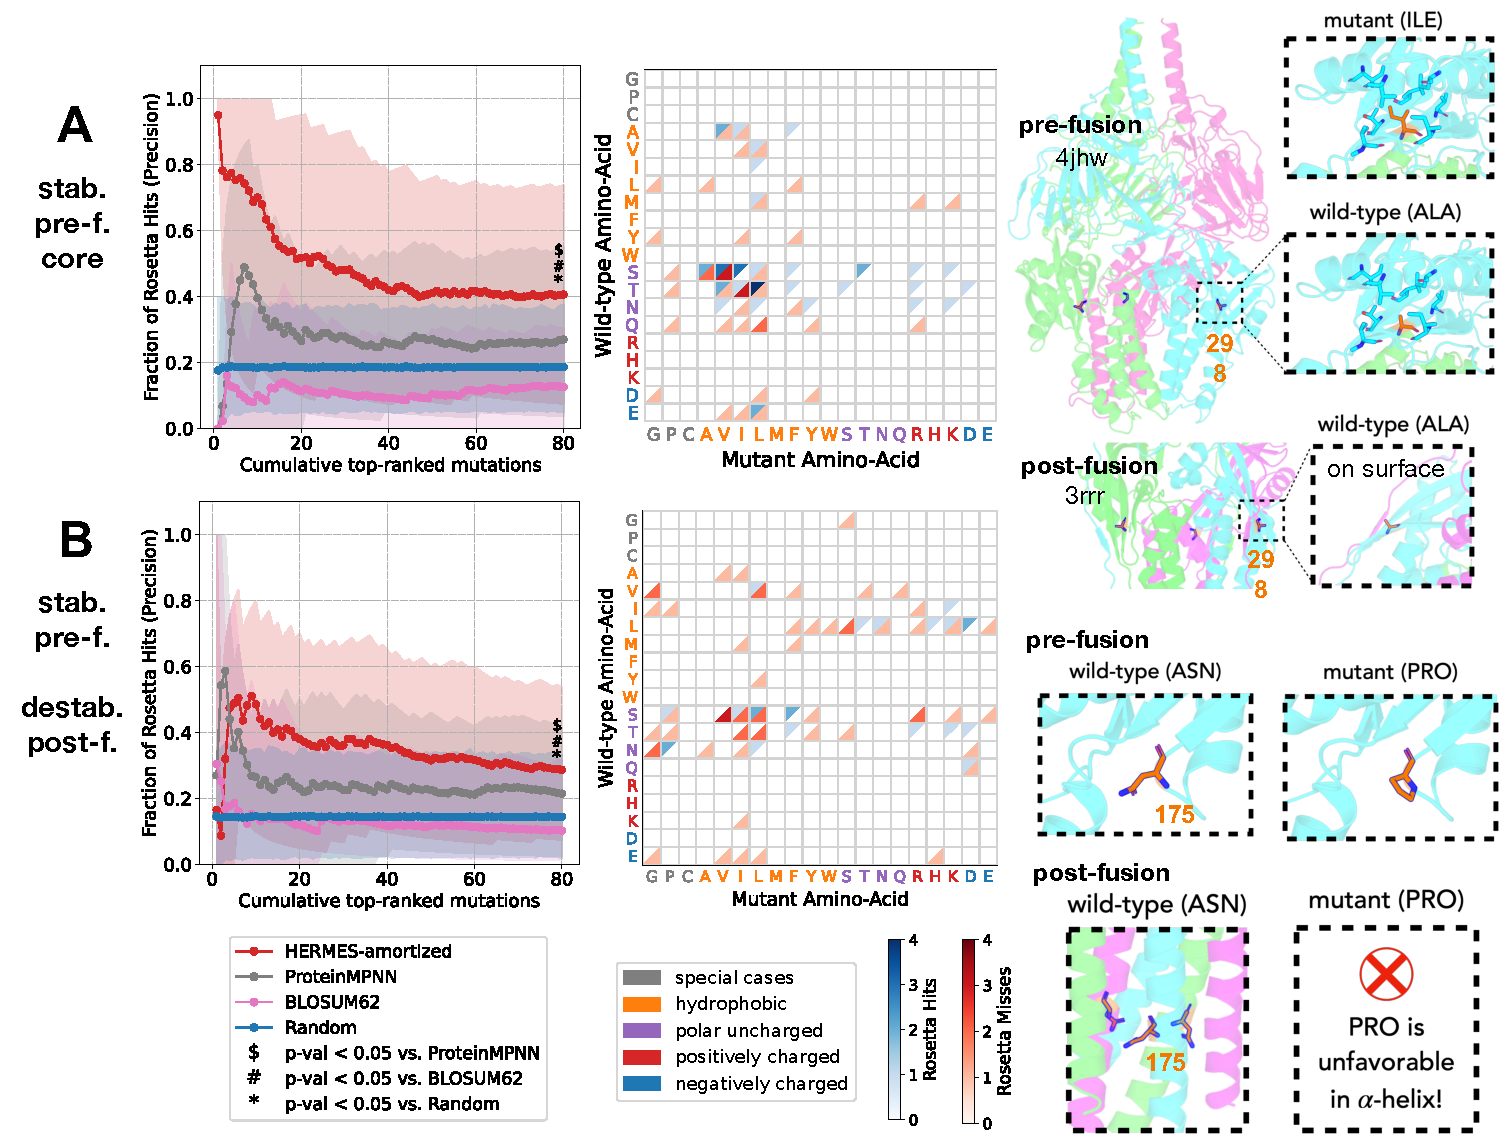
\includegraphics[width=1.0\linewidth]{figures/rsv_f_rosetta_hits_main_figure.pdf}
    \figcaption{\GM{Identifying new antigen-stabilizing mutations with HERMES for RSV-F.}}{
    \GM{
    Panel {\bf A} shows results using the ``stabilize pre-fusion core" pipeline, whereas
    panel {\bf B} shows results using the ``stabilize pre-fusion and destabilize post-fusion" pipeline.
    Each panel is split in three sub-panels.
    \textit{Left}: Rosetta hit rate as a function of number of top-$k$ suggested mutations
    (for all methods except for Random, for which we show the average hit rate of 20 random samples of $k$ mutations from the pool
    of 160 randomly-selected mutations).
    Rosetta hits were computed multiple times via 200 bootstrap samples with replacement of the 50 REU
    scores.
    Solid lines and markers denote the mean across bootstrap samples, whereas shaded regions denote
    the 5-95 percentile range.
    We note that all BLOSUM62 suggestions had a score $\geq 1$ and are ranked by score just like HERMES and ProteinMPNN.
    P-values were computed via Wilcoxon signed-rank test and corrected for multiple testing via
    Bonferroni within each panel.
    \textit{Center}: heatmap showing number of Rosetta hits (blue) and misses (red) for each amino-acid
    mutation pair suggested by HERMES-{\em amortized}.
    Here, Rosetta hits were computed using all 50 REU scores instead of bootstrap samples.
    \textit{Right}: examples of promising antigen-stabilizing mutation identified by each pipeline.
    Mutant structures were generated using PyMOL's protein mutagenesis wizard.
    }
    }
    \label{fig:rsv_f_rosetta_hits_main_figure}
\end{figure}


\begin{table}[t!]
\centering
\begin{tabular}{l | c c | c c}
\toprule
 & \textbf{Per-Struct.} & \textbf{Per-Struct.} & \textbf{Overall} & \textbf{Overall} \\
\textbf{Method} & \textbf{Pearson} & \textbf{Spearman} & \textbf{Pearson} & \textbf{Spearman} \\
\midrule
Rosetta$^*$~\citep{park_simultaneous_2016} & 0.328 & 0.299 & 0.311 & 0.347 \\
FoldX$^*$~\citep{delgado_foldx_2019} & 0.391 & 0.364 & 0.356 & 0.351 \\
\midrule
DDGPred$^*$~\citep{shan_deep_2022} & 0.371 & 0.343 & 0.652 & 0.439 \\
ESM-IF$^*$~\citep{hsu_learning_2022} & 0.231 & 0.209 & 0.296 & 0.287 \\
MIF-Net.$^*$~\citep{luo_rotamer_2022} & 0.395 & 0.348 & 0.667 & 0.480 \\
RDE-Net.$^*$~\citep{luo_rotamer_2022} & 0.469 & 0.433 & 0.642 & 0.527 \\
\midrule
Vanilla Pythia PPI$^\dagger$~\citep{tao_reliable_2025} & 0.478 & 0.449 & 0.709 & 0.537 \\
Pythia-PPI$^\dagger$~\citep{tao_reliable_2025} & 0.565 & 0.527 & 0.785 & 0.637 \\
\midrule
\midrule
\proteinmpnn & 0.281 & 0.282 & 0.331 & 0.315 \\
\proteinmpnnNoise & 0.270 & 0.255 & 0.334 & 0.289 \\
\HERMESPy & 0.306 & 0.287 & 0.285 & 0.272 \\
\HERMESPyNoise & 0.317 & 0.308 & 0.291 & 0.286 \\
\HERMESPyFtRelaxed & 0.231 & 0.241 & 0.290 & 0.242 \\
\HERMESPyNoiseFtRelaxed & 0.222 & 0.239 & 0.276 & 0.222 \\
\HERMESPyFtCdna & 0.347 & 0.331 & 0.380 & 0.342 \\
\HERMESPyNoiseFtCdna & 0.305 & 0.294 & 0.344 & 0.288 \\
\midrule
\HERMESPyFtSkempiEasy & 0.471 & 0.433 & 0.578 & 0.476 \\
\HERMESPyNoiseFtSkempiEasy & 0.430 & 0.389 & 0.512 & 0.420 \\
\HERMESPyFtSkempiMedium & 0.472 & 0.430 & 0.576 & 0.466 \\
\HERMESPyNoiseFtSkempiMedium & 0.407 & 0.368 & 0.497 & 0.403 \\
\HERMESPyFtSkempiHard & 0.435 & 0.398 & 0.395 & 0.380 \\
\HERMESPyNoiseFtSkempiHard & 0.399 & 0.359 & 0.328 & 0.322 \\
\bottomrule
\end{tabular}
\figcaption{Benchmark on predicting mutational effects on protein-protein binding in SKEMPI.}{
The Spearman/Pearson correlations between model-predicted effects of single point mutations and
experimental values from the SKEMPI v2.0 dataset~\citep{jankauskaite_skempi_2019} are reported both
across mutations within each structure individually (``per-structure" correlations), and over
mutations pooled across all complexes (``overall" correlations). Entries marked with $*$ are taken
from ref.~\citep{luo_rotamer_2022} and, for machine learning-based methods (all except Rosetta and
FoldX), were obtained using 3-fold cross-validation over SKEMPI complexes.
Entries marked with $\dagger$ are taken from ref.~\citep{tao_reliable_2025}, and were obtained via
5-fold coss validation on the SKEMPI complex structures.
We evaluate HERMES using three train/test splits defined from SKEMPI metadata, with increasing
difficulty: (i) {\em Easy}, a random split; (ii) {\em Medium}, which groups sites with similar
binding sites (hold-out proteins) into the same split; (iii) {\em Difficult}, which groups sites
from the same held-out protein types (functional classes) into the same split (see Extended Methods,
Appendix~\ref{sec:hermes_appendix} for details).
The HERMES models with most comparable training procedure to the other machine learning models are
those fine-tuned on the \textit{Easy} split, for which we used 3-fold cross-validation with splits
defined by PDB complex.
Note that, similar to HERMES, the machine learning models in ref.~\citep{luo_rotamer_2022} were
fine-tuned on SKEMPI $\Delta\Delta G_{\text{binding}}$ labels only, whereas Pythia-PPI
\citep{tao_reliable_2025} was trained on a mixture of SKEMPI binding labels and FireProtDB stability
labels \citep{stourac_fireprotdb_2021} and further refined via self-distillation.
}
\label{table:skempi_spm}
\end{table}

\subsection{Predicting {binding} effect of mutations}
Predicting the effects of mutations on binding affinity is a central step in target-specific protein
design. In prior work, we demonstrated the utility of HERMES for predicting how mutations in short
peptide antigens alter binding to T-cell receptors in the context of MHC
complexes~\citep{visani_t_2025}. We further leveraged this capability for de novo design of peptide
antigens intended to elicit specific T-cell responses~\citep{visani_t_2025}. Here, we evaluate
HERMES on the single-point mutation effects from the SKEMPI v2.0
dataset~\citep{jankauskaite_skempi_2019}, which spans a substantially broader range of
protein-protein interactions and binding-affinity perturbations.

In a zero-shot setting, HERMES exhibits measurable predictive signal (HERMES-\emph{fixed} 0.50;
Spearman's $\rho = 0.286$). ProteinMPNN achieves comparable overall performance, whereas
physics-based approaches (Rosetta~\citep{chaudhury_pyrosetta_2010} and
FoldX~\citep{schymkowitz_foldx_2005}) perform modestly better (Spearman's $\rho \approx 0.35$). In
contrast to our results for stability prediction, HERMES-\emph{fixed} models correlate more strongly
with binding effects than HERMES-\emph{amortized} models. Interestingly, fine-tuning for stability
(HERMES-\emph{fixed} 0.00+ cDNA117k) yields a slight improvement in binding-effect prediction. A
detailed comparison across models is provided in Table~\ref{table:skempi_spm}.

Next, we fine-tuned HERMES directly on SKEMPI using 3-fold cross-validation. To control for
information leakage under structural similarity, we introduced three homology-aware splitting
strategies of increasing difficulty; the most stringent split prevents complexes from the same
interaction ``class" (e.g., antibody-antigen or TCR-pMHC) from appearing in different folds; see
Extended Methods, Appendix~\ref{sec:hermes_appendix} for details.
Fine-tuned HERMES models achieve substantially stronger correlations, including
under the {\em Difficult} split (Table~\ref{table:skempi_spm}).

Finally, we compared HERMES to recent state-of-the-art methods, RDE-Network and
MIF-Network~\citep{luo_rotamer_2022}, DDGPred~\citep{shan_deep_2022},
ESM-IF~\citep{hsu_learning_2022} and Pythia-PPI~\citep{tao_reliable_2025}. These baselines were also
trained on SKEMPI using 3- or 5-fold cross-validation under protocols analogous, but not identical,
to our {\em easy} split. HERMES fine-tuned on SKEMPI-Easy performs competitively with RDE-Network
and MIF-Network, but trails Pythia-PPI (Table~\ref{table:skempi_spm}). Notably, RDE-Network and
MIF-Network are fine-tuned on SKEMPI $\Delta\Delta G$ labels in a manner similar to our approach,
whereas Pythia-PPI incorporates additional training procedures that further boost performance
(Extended Methods, Appendix~\ref{sec:hermes_appendix}). These procedures are, in principle, applicable
to HERMES as well, but we leave a
systematic evaluation of such extensions, and of HERMES as a general framework for binding-affinity
prediction, to future work.


\section{Summary}

In this chapter, we introduced HERMES, a family of fast, structure-based machine learning models for predicting the
effects of mutations on protein function. HERMES leverages SO(3)-equivariant neural networks
operating on local atomic neighborhoods in a protein structure to predict amino acid propensities,
whose differences can be used to predict mutational effects. This formulation yields a
computationally efficient predictor that is naturally suited to high-throughput settings. HERMES
captures mutational impacts on diverse phenotypes, including thermodynamic stability and
protein-protein binding affinity, and it provides a practical tool for antigen stabilization in
vaccine design.

A central finding is that encoding packing flexibility is essential for accurate predictions across
mutations involving amino acids of different sizes. HERMES-{\em fixed}, a lightweight protocol that
evaluates mutations in the rigid wild-type structure, exhibits strong bias toward size-conserving
substitutions. Explicitly modeling relaxation via Rosetta~\citep{chaudhury_pyrosetta_2010},
(HERMES-{\em relaxed} protocol) resolves this bias but incurs substantial computational cost. Our
amortized approach offers an effective compromise: by fine-tuning on relaxed predictions for just
0.5\% of pre-training data, HERMES-{\em amortized} learns implicit packing flexibility that can be
leveraged for predictions at HERMES-{\em fixed} speed. This capability proves particularly valuable
for antigen stabilization, where HERMES-{\em amortized} recovers over half of the verified
stabilizing mutations in our benchmark and shows strong performance on proline substitutions (87.5\%
recovery), which stabilize proteins by restricting backbone conformational freedom.

Beyond zero-shot use, HERMES can be fine-tuned directly on experimental labels using a simple
end-to-end procedure. Notably, both the native and the fine-tuned models use the difference of amino
acid scores for predicting mutational effects, which yields an inherent reversibility with respect
to mutation order--a thermodynamic consistency property that is often enforced via explicit
19$\times$ data augmentation~\citep{diaz_stability_2024}.

With fine-tuning, HERMES achieves competitive accuracy on thermodynamic stability benchmarks when
trained on the same data as prior methods~\citep{blaabjerg_rapid_2023, diaz_stability_2024,
dieckhaus_transfer_2024}. Interestingly, stability fine-tuning does not consistently transfer to
antigen stabilization and can even degrade performance. One plausible explanation is dataset
mismatch: the high-throughput stability datasets used for
fine-tuning~\citep{tsuboyama_mega-scale_2023} are enriched for relatively small, compact domains,
whereas vaccine antigens are often larger, multi-domain, and conformationally heterogeneous, with
stabilizing mutations frequently targeting quaternary contacts, glycoprotein-specific features, or
prefusion-state constraints. Resolving this discrepancy will likely require broader supervision that
better reflects antigen structure and design objectives, or task-aligned fine-tuning data.

We also demonstrate that pre-training on wild-type amino acid classification remains necessary for
strong performance; models trained only on currently-available experimental stability data fail.
Notably, pre-trained models exhibit ``wild-type preference," assigning elevated probabilities to
wild-type residues in wild-type structural contexts. This bias correlates with sequence similarity
to pre-training proteins, suggesting partial memorization rather than purely generalizable learning.
Fine-tuning partially ameliorates but does not eliminate this effect, representing a fundamental
trade-off in current training paradigms. More robust pre-training objectives, stronger
regularization, or explicit debiasing strategies may be required to fully address this issue.

A key application we highlight is structure-based vaccine design, where practitioners seek to
stabilize substitutions that preserve a desired prefusion conformation of a vaccine antigen to
elicit immune responses targeting relevant epitopes. For this task, a useful model should propose
stabilizing mutation candidates across different sites of an antigen.
On the limited available data comprising 33 verified antigen-stabilizing mutations across five viruses,
HERMES performs well in recovering these mutations.
\GM{We also develop two pipelines to suggest mutations with HERMES across the full antigen,
showing close agreement with predictions made with the physics-based model Rosetta, which we
suggest to use to further filter the candidate set of mutations.}
Moreover, the strict locality of the model makes it straightforward and
fast to apply to large antigens and assemblies that can pose challenges for architectures modeling
global interactions in proteins.
Our results show that local all-atom environments modeled by HERMES
can encode multiple stabilization mechanisms, including cavity filling, post-fusion disruptions and
pre-fusion backbone rigidification via prolines, and favorable electrostatic remodeling,
while also underscoring limitations for mechanisms
that depend on long-range coupling, or multi-site epistasis.


We further evaluated HERMES on predicting changes in protein--protein binding affinity using the
SKEMPI dataset~\citep{jankauskaite_skempi_2019}. In the zero-shot setting, HERMES shows measurable
predictive signal, and supervised fine-tuning on SKEMPI {substantially} improves performance.
Recent state-of-the-art approaches for binding prediction like Pythia-PPI~\citep{tao_reliable_2025}
indicate that design choices such as self-distillation can substantially improve
performance~\citep{tao_reliable_2025}; we expect HERMES would similarly benefit from such
approaches, representing a clear next step.

Several directions could extend HERMES' capabilities. Developing larger, more diverse training
datasets, particularly for antigen stabilization and binding, would likely improve performance, as
our results indicate that training data dominates architectural differences in determining benchmark
performance. The locality of HERMES appears to be a double-edged sword: local neighborhoods reduce
input complexity, remove constraints on protein size, and improve scalability, but necessarily limit
the model's ability to capture long-range epistasis and allosteric coupling. We view HERMES as a
hypothesis-generation tool whose predictions are most reliable when mutational effects are driven
primarily by short-range interactions and local packing. Productive directions for future work
include better characterizing when locality suffices, further reducing pre-training-induced biases,
and developing multi-scale approaches that efficiently combine local all-atom predictors with
complementary global or multi-site models to capture mechanisms beyond the local neighborhood.



\chapter{Mapping the T-cell receptor specificity landscape with HERMES}
\label{sec:tcrpmhc}

T-cells play a key role in the adaptive immune system, contributing to immune surveillance and
response to pathogens. T-cells recognize pathogen-derived epitopes in the form of short protein
fragments (peptides) displayed on specific molecules known as Major Histocompatibility Complexes
(MHCs). The binding between a T-cell receptor (TCR) and a peptide-MHC (pMHC) is essential to mediate
a protective T-cell response to an infection. To defend the host against a multitude of pathogens, a
highly diverse TCR repertoire is generated through a somatic VDJ recombination process, and selected
to target infected cells with remarkable sensitivity and specificity.

Predicting the TCR-pMHC binding specificity is an important step in characterizing the efficacy of
the immune system in countering different pathogens. Such understanding would aid with disease
diagnoses and development of diagnostic tests for early detection of autoimmune
diseases~\cite{Attaf2015-tw}. A predictive model for TCR-pMHC specificity can be used to design
engineered TCRs that recognize cancer antigens~\cite{Liu2025-hl}, enhancing the effectiveness of
adoptive cell transfer and {Chimeric Antigen Receptor (CAR) T-cell}
therapies~\cite{Leidner2022-ca,Mirazee2024-bo}, as well as the design of soluble TCRs and bispecific
T-cell engager therapeutics~\cite{Hsiue2021-ag}. Moreover, it can enable the design of optimized
antigens for vaccines to elicit robust T-cell responses against specific pathogens or
tumors~\cite{Sahin2018-fv,Blass2021-jd,Rojas2023-nx}.

One bottleneck in deciphering the TCR-pMHC code is the lack of well-curated datasets.
High-throughput immune repertoire sequencing, combined with comparative analyses of hosts facing
similar immune challenges, and the development of functional assays (e.g., {pMHC-tetramer
staining}~\cite{Zhang2018-pe} or MIRA~\cite{Nolan2025-fu}), have enabled the identification of
diverse TCR pools with potential reactivity to specific antigens~\cite{Dash2017-if}, collected in
repositories like Immune Epitope Database (IEDB)~\cite{Vita2019-qn} and VDJdb~\cite{Shugay2018-nt}.
However, the current databases are unbalanced, with only a handful of dominant peptides (e.g.
derived from SARS-CoV-2, CMV, EBV, Influenza, etc.) and {MHC alleles} present, each linked to
hundreds of TCRs.

As a result, statistical inference and machine learning methods trained on such data to predict
TCR-pMHC reactivities lack generalizability beyond their training
data~\cite{Isacchini2021-fs,Weber2021-ik,Meynard-Piganeau2024-po}. On the structural side, only a
few hundred TCR-pMHC crystal structures have been experimentally generated to date. This is in part
because TCR-pMHC interactions are typically of low affinity and are difficult to stabilize to the
level needed for CryoEM or X-ray crystallography~\cite{Piepenbrink2009-jy}. Importantly, this
scarcity hinders computational prediction methods like AlphaFold in modeling reliable TCR-pMHC
structures~\cite{Bradley2023-rl,Yin2023-zm}. Machine learning models, such as large language models,
pre-trained on vast unannotated protein datasets can generate meaningful data
representations~\cite{Rives2021-sr,Lin2023-ub}. Fine-tuning these models on smaller, labeled
datasets for specific tasks (e.g., predicting mutation impacts on stability or function) has proven
highly effective~\cite{Madani2023-mg,Schmirler2024-wp,Wang2024-ep,Hie2024-vb}. Pre-trained
sequence-based protein language models have been employed to predict reactivities of antibodies to
antigens~\cite{Wang2024-ep,Hie2024-vb}, or TCRs to pMHC
complexes~\cite{Bravi2023-aj,Meynard-Piganeau2024-po}. However, lack of generalizability due to
sparse and skewed training data has remained a challenge in these models.

 
\begin{figure*}[th!]

\includegraphics[width=1.0\textwidth]{tcrpmhc/figures/schematic_0}
\figcaption{HERMES model for predicting and designing TCR-pMHC interactions.}{ {\bf (A)} HERMES is
a structure-based, rotationally equivariant neural network pre-trained on the protein universe to
predict amino acid preferences at a residue from its 3D structural
environment~\cite{Visani2024-sh,Pun2024-qz}. It takes as input all atoms within 10\AA\ of a focal
residue (with that residue’s atoms masked), featurizing them by atom type, charge, and SASA. HERMES
then outputs energies $E_i(\sigma)$ for the 20 possible amino acids $\sigma$ at residue $i$, which
serve as logits in a softmax to estimate amino acid likelihoods.
{\bf (B)} To predict TCR-pMHC affinity, we use two protocols: HERMES-{\em fixed} (left) and
HERMES-{\em relaxed} (right). In HERMES-{\em fixed} we use a fixed structural template closest to
the TCR-pMHC of interest as input to HERMES, and evaluate the peptide energy as the sum of
HERMES-computed per-residue energies for the peptide. In HERMES-{\em relaxed} mutations are
introduced to the template's peptide to match the peptide of interest, followed by local repacking
in PyRosetta~\cite{Chaudhury2010-mo}. Peptide energy is then evaluated similar to HERMES-{\em
fixed}, but using the relaxed structure. {\bf (C)} We also use two protocols for peptide design.
Similar to (B) we fix the closest structural template in HERMES-{\em fixed}, and use HERMES'
likelihood matrix for possible amino acids at each peptide position, which we sample to generate new
peptide sequences. In HERMES-{\em relaxed} (right), we begin with a random peptide $\sigma$, and
locally pack it with PyRosetta, and also generate an amino acid likelihood matrix (similar to
HERMES-{\em fixed}) for this packed structure. We sample a new sequence $\sigma'$ from this
likelihood matrix, and pack it with PyRosetta. We evaluate peptide energies
$E_{\text{peptide}}(\sigma)$, and $E_{\text{peptide}}(\sigma')$ for both peptides, using their
respective PyRosetta-relaxed structures, and we use these energies as the criterion to sample
improved sequences with MCMC (SI). This procedure is then iterated until convergence. Peptides
designed by both approaches are then filtered by TCRdock~\cite{Bradley2023-rl} or Alpha-Fold
3~\cite{Abramson2024-jp} to assure the stability of the complex.
\label{Fig:1}}
\end{figure*}
 
Protein-protein interactions in general, and immune-pathogen interaction in particular, rely on the
complementarity in the 3D structures and amino acid compositions of the interacting protein pairs.
Even though the interacting amino acids can be far apart in a protein sequence, they are close to
each other in structure, resulting in local interactions that can determine immune-pathogen
recognition. Machine learning models trained on protein structures instead of sequences can learn
local structural representations for amino acid statistics, which tend to be more generalizable
across different protein families and beyond their training
sets~\cite{Dauparas2022-fu,Blaabjerg2023-oq,Michalewicz2024-hw,Visani2024-sh,Pun2024-qz,Diaz2024-vv}.

Here, we present a structure-based approach to predict interaction affinities between TCRs and
peptides presented on {MHC class I}, and to design reactive peptides for specific TCR-MHC-I
complexes (TCR-MHC for short). Due to the limited availability of structural data for TCRs, we use
HERMES-- a physics-guided, 3D-equivariant machine learning model trained on the entire protein
universe to predict amino acid preferences based on their local structural
environments~\cite{Pun2024-qz,Visani2024-sh}.
 
{We demonstrate that HERMES accurately predicts both binding affinity of TCR-pMHC Class I complexes
and the functional responses and T-cell activities induced by a range of peptides presented on MHC
molecules. Affinity of TCR-pMHC complexes, measured as the dissociation constant $K_d$ by surface
plasmon resonance, is labor intensive to obtain. Functional readout used to measure T-cell
activities, including measurements of T-cell proliferation, labeled cellular activation markers, and
cytokine (e.g., IFN-$\gamma$) release, are easier to obtain than affinity measurements. Yet,
functional readouts are shaped not only by the TCR-pMHC affinity, but also by other cellular factors
such as the T-cell's differentiation state (e.g., naive or memory), self-reactivity of the
TCR~\cite{Altan-Bonnet2005-lm,Achar2022-tb}, and the avidity effects driven by TCR/co-receptor
clustering and pMHC density on antigen-presenting cells~\cite{Stone2009-ab}. Although HERMES is more
suited to predict molecular affinities, we show that its scores nonetheless can well track T-cell
activities, making it a reliable tool for predicting T-cell response to antigens.}

Lastly, we show that HERMES can be used to design novel peptides {binding specific} TCR-MHC
complexes, achieving up to 50\% experimental validation accuracy across diverse TCR-MHC systems.
%Our peptide design platform can facilitate the computational design of {neoantigen} libraries for
cancer vaccines.
By leveraging our design algorithm, we characterize the specificity of a diverse range of {TCRs},
providing a quantitative measure for the diversity of the peptide-MHC antigens that a TCR can
recognize in humans and mice.

\begin{figure*}[ht!]
	\centering
	
\includegraphics[width=0.9\textwidth]{tcrpmhc/figures/affinity_figure_0}
	\figcaption{Predicting binding affinity of TCR-pMHC complexes.}{ {\bf(A)} The structure of the
	NY-ESO-1
	peptide (purple), in complex with HLA-A*02:01 and a purified specific 1G4 TCR is shown (PDB ID:
	2BNQ~\cite{Chen2005-jk}). This structure together with that of a peptide variant with C9V mutation
	(PDB ID: 2BNR~\cite{Chen2005-jk}) are used as templates to predict the binding affinity of the
	TCR-MHC complex to other peptide variants. {\bf (B)} The binding affinities ($-\log_{10}
	(K_d/\mu\text{M})$) of TCR-MHC complexes with 14 distinct peptides, measured using surface plasmon
	resonance, are shown against the predicted HERMES-{\em relaxed} peptide energies, using the closest
	structural template for each variant; 2BNQ is used for blue points and 2BNR for the orange point.
	The Spearman $\rho$ between predictions and measurements is reported in the panel. {\bf(C)} The
	heatmaps show the experimental affinity values (top) and predicted peptide energies (bottom) for
	all the peptide variants, with the identity of the mutations color coded based on the closest
	structural template. {\bf(D-F)} Similar to (A-C) but for the Tax viral peptide in complex with
	HLA-A*02:01 and a specific human TCR. Two structural templates are used~\cite{Garboczi1996-fr} for
	evaluating peptide energies with PDB IDs: 1AO7 (shown in D, and used for blue points), and 1QSF
	(used for orange points).
	\label{Fig:2}
	}
\end{figure*}

\section*{Model}

 T-cell response is mediated by the interactions between TCRs and pMHC complexes. To model the
 TCR-pMHC interaction, we use HERMES~\cite{Visani2024-sh}, a 3D rotationally equivariant
 structure-based neural network model, trained on the protein universe; see Fig.~\ref{Fig:1}A.
HERMES predicts the amino acid propensity from its surrounding 3D protein environment, a measure
that we have previously shown to serve as a reliable proxy for assessing the effect of mutations on
protein stability or binding~\cite{Pun2024-qz,Visani2024-sh}.

For TCR-pMHC complexes, we seek to determine how changes in a peptide sequence impact the binding
affinity of a TCR-pMHC complex, and ultimately, the T-cell response to the antigen. To do so, we
characterize a score, which we term peptide energy, for a peptide $\sigma$, given its surrounding
TCR and MHC structural environment,
{
\EQ
E_{\text{peptide}}(\sigma ; \text{TCR, MHC}) = \sum_{i=1}^\ell E(\sigma_i ; \text{TCR,
MHC},\sigma_{/i})
\label{eq:pepEn}
\EE
We assume that each peptide residue contributes linearly to the total energy by the amount
$E(\sigma_i ; \text{TCR, MHC}, \sigma_{/i})$, where $\sigma_i$ is the amino acid at position $i$ of
the peptide. A residue's energy contribution $E$ is evaluated by HERMES (logits of the network),
taking in as input the atomic composition of the surrounding TCR, MHC, and the rest of the peptide
$\sigma_{/i}$ (excluding the $i^{th}$ residue) within a 10~\AA~of $\sigma_i$'s $\alpha$-Carbon}; see
Fig.~\ref{Fig:1} and SI for details.

\begin{table*}[ht]
\centering
\begin{tabular}{ll|cc|cccccccc}
\toprule
 & & \multicolumn{2}{c|}{TCR-pMHC affinity} & \multicolumn{8}{c}{T-cell activity} \\
\cmidrule(lr){3-4}\cmidrule(lr){5-12}
Model type & Model & 1G4 TCR & A6 TCR & H2-scDb & TCR1 & TCR2 & TCR3 & TCR4 & TCR5 & TCR6 & TCR7 \\
\midrule
\multirow{1}{*}{Substitution Matrix} & BLOSUM62~\cite{Henikoff1992-jq} & \textbf{\underline{0.83}} &
{0.56}* & -0.05 & -0.07 & 0.14 & 0.38 & \textbf{\underline{0.33}} & 0.42* &
\textbf{\underline{0.55}} & -0.01 \\
\midrule
\multirow{2}{*}{Structure Prediction} & TCRdock~\cite{Bradley2023-rl} & {0.62*} &
\textbf{\underline{0.88}} & N/A & 0.02 & 0.13 & 0.21 & 0.18* & -0.02 & 0.19 & 0.06 \\
& TCRdock-{\em no template}~\cite{Bradley2023-rl} & 0.25 & -0.14 & N/A & -0.03 & 0.44 & 0.11 & -0.22
& 0.28* & 0.14 & 0.06 \\
\midrule
\multirow{1}{*}{Sequence based ML} & TAPIR~\cite{Fast2023-tk} & 0.29 & 0.35 & N/A & 0.36 & 0.36 &
-0.00 & 0.12 & 0.39* & 0.08 & -0.01 \\
\midrule
\multirow{2}{*}{Structure based ML} 
& ESM-IF1~\cite{Hsu2022-km} & 0.38* & 0.17 & 0.12 & 0.43* & 0.41 & 0.19 & -0.15 & 0.28* & 0.25 &
0.08 \\
& ProteinMPNN~\cite{Dauparas2022-fu} & -0.01 & 0.49 & \textbf{\underline{0.55}} & 0.46* & 0.52 &
0.49* & -0.28 & \textbf{\underline{0.45}} & 0.41* & \textbf{\underline{0.31}} \\
\midrule
\multirow{2}{*}{Structure based ML} & HERMES-\textit{fixed} & 0.29 & 0.63* & 0.46* &
\textbf{\underline{0.56}} & \textbf{\underline{0.71}} & \textbf{\underline{0.59}} & -0.06 & 0.37* &
0.42* & -0.01 \\
& HERMES-\textit{relaxed} & 0.72* & 0.56* & 0.29 & 0.31 & 0.57 & 0.55* & -0.20 & 0.37* & 0.42* &
0.14* \\
\bottomrule
\end{tabular}
\figcaption{Benchmarking of models for predicting TCR-pMHC binding affinities and T-cell
activities.}
{The table lists the Spearman~$\rho$ of models' predictions against experimentally
measured binding affinities (Fig.~\ref{Fig:2}) and T-cell activities (Fig.~\ref{Fig:3}) in response
to peptide variants. The HERMES-{\em fixed} and HERMES-{\em relaxed} performance are from models
with no noise (0.00) in training data, and the ProteinMPNN performance is from the model with a
small noise amplitude of 0.02~\AA; see SI for details. We show in \textbf{bold} the best model for
each dataset, and any model whose performance is \textit{not} significantly different from the best
model (p-value$>0.05$ associated with the difference in the Fisher's z-transformed Spearman
correlations) is indicated with an asterisk (*). See
Tables~\SpearmanrAffinityTable~and~\SpearmanrActivityTable~in the SI for $p$-values and additional
models.}
\label{table:spearmanr_affinity_and_activity}
\end{table*}


 To compute peptide energy, we input to HERMES an experimentally or computationally determined
 structure of a specified TCR-MHC complex bound to at least one peptide variant. Experimental data
 on the impact of peptide substitutions on the TCR-pMHC structure is limited, and computational
 models often fail to capture subtle conformational changes in the structure due to amino acid
 substitutions in a peptide. Given these constraints, we adopt two approaches to estimate peptide
 energies across diverse peptide variants for a given TCR-MHC complex:
\begin{itemize}
	\item HERMES-{\em fixed}: In the simplest approach, we choose a TCR-pMHC structure with the same
	TCR and MHC as our query and a peptide sequence closest to the peptide of interest. This structure
	is then used as our template in HERMES to compute the peptide energy as described in
	eq.~\ref{eq:pepEn} (Fig.~\ref{Fig:1}B). This method does not alter the underlying structure and
	assumes that peptide amino acid substitutions do not significantly change the conformation of the
	TCR-pMHC complex.
	
	\item HERMES-{\em relaxed}: Since amino acid substitutions can locally reshape a protein complex,
	we introduce a more involved protocol to account for these structural changes. We begin with the
	closest available structure for the TCR-pMHC complex. We then mutate the original peptide to the
	desired state and apply a relaxation procedure using PyRosetta to pack the substituted amino
	acid~\cite{Chaudhury2010-mo} (SI). During relaxation, side-chain and backbone atoms of the peptide
	are allowed to move, while only the side-chain atoms of the MHC and TCR chains within a
	10~\AA\,radius of the peptide are flexible. We then calculate the peptide energy with HERMES
	(eq.\ref{eq:pepEn}), using the relaxed structure as input (Fig.~\ref{Fig:1}B). Since PyRosetta's
	relaxation procedure is stochastic, we average the peptide energy across 100 realizations of these
	relaxations. {For ablation purposes, we also include results obtained by selecting the relaxed
	conformation with the lowest (most favorable) Rosetta energy, and using its HERMES peptide energy.}
\end{itemize}





\section*{Results}
\subsection*{Predicting binding affinity of TCR-pMHC complexes} 
 Binding between TCRs and pMHC complexes is necessary to mediate a T-cell response. The binding
 affinity of a natural TCR-pMHC complex is relatively low, with a dissociation constant $K_d$ in the
 range of $1-100\mu{\rm M}$~\cite{Davis1998-bv,Piepenbrink2009-jy,Zhong2013-ja}, in contrast to
 nanomolar affinities for antibody-antigen complexes. Engineered TCRs can achieve much higher
 affinities in a nanomolar~\cite{Soto2013-df} to picomolar~\cite{Li2005-md, Dunn2006-dh} range.

Surface plasmon resonance (SPR) spectroscopy provides accurate measurements of the dissociation
constant ($K_d$) for specific TCR-pMHC systems. In these experiments, one protein--either the TCR or
the MHC--is immobilized on a conducting plate, and the other is introduced in solution to bind to
it. This binding alters the local refractive index near the plate, affecting the resonance signal.
We {used a published} dataset of SPR-measured affinities for two TCR-MHC complexes binding to an
ensemble of peptides, for which crystal structures of the complexes with at least one peptide are
available~\cite{Aleksic2010-wz,Pettmann2021-kl}; see Table~\AffActInfoTable~for details.

In our first example, we examined TCR 1G4 binding to NY-ESO-1 peptide variants, which is a
cancer-testis antigen commonly expressed in many cancers and is targeted by
immunotherapies~\cite{Esfandiary2015-jf}. We used two structural templates, one with the wild-type
peptide SLLMWITQC (NY-ESO-1), and the other with a more immunogenic peptide, in which the Cysteine
at position 9 is substituted by Valine (C9V)~\cite{Chen2000-vq,Chen2005-jk} (Fig.~\ref{Fig:2}A). For
variants differing by a single amino acid, our predictions with HERMES-{\em relaxed} correlated well
(Spearman {$\rho=0.72$}) with experimentally measured affinities from
refs.~\cite{Aleksic2010-wz,Pettmann2021-kl}; see Fig.~\ref{Fig:2}B,~C.

Next, we tested the A6 TCR binding to the HTLV-1 Tax peptide LLFGYPVYV. We employed two structural
templates: one with the wild-type, the other with the mutant peptide with substitution
Y8A~\cite{Garboczi1996-fr} (Fig.~\ref{Fig:2}D and {Table~\AffActInfoTable}). Again, the HERMES-{\em
relaxed} peptide energies correlated well (Spearman {$\rho=0.56$}) with the affinities, measured in
ref.~\cite{Pettmann2021-kl} (Fig.~\ref{Fig:2}E,~F).

{Overall, HERMES predictions aligned closely with these limited experimental affinity measurements,
with HERMES-{\em relaxed} showing a better agreement with affinity measurements than HERMES-{\em
fixed}.
We compared our approach for scoring peptides to alternative methods, including the baseline
substitution matrices (BLOSUM62~\cite{Henikoff1992-jq} and the TCR-specific substitution matrices
from ref.~\cite{Luksza2022-gx}), the score from the TCR-pMHC structure prediction algorithm
TCRdock~\cite{Bradley2023-rl}, the sequence-based machine learning algorithms for TCRs
(TAPIR~\cite{Fast2023-tk}, NetTCR~\cite{Jensen2024-xs}, and TULIP~\cite{Meynard-Piganeau2024-po}),
and the structure-based inverse folding models (ESM-IF1~\cite{Hsu2022-km} and
ProteinMPNN~\cite{Dauparas2022-fu}); see Table~\ref{table:spearmanr_affinity_and_activity} for key
benchmarking results and Table~\SpearmanrAffinityTable~and Fig.~\ProteinMPNNScoringSchemesFigure~for
a more extensive comparison of different methods, including the different HERMES models, and
different scoring schemes by ProteinMPNN.
 
For the 1G4 TCR, BLOSUM62~\cite{Henikoff1992-jq} achieves the highest correlation with experimental
affinity data, whereas template-guided TCRdock~\cite{Bradley2023-rl} leads for the A6 system; in
contrast, TCRdock without using a homologous structure as a template underperforms. In both systems,
HERMES achieves performance that is statistically indistinguishable from the top performers
(Fisher's z-test p-value $>0.05$). Overall, BLOSUM62, template-guided TCRdock, and HERMES rank
strongly as predictors of TCR-pMHC affinities across the tested datasets. In addition, for the 1G4
system, ESM-IF1~\cite{Hsu2022-km} and the TCR-specific substitution matrices from
ref.~\cite{Luksza2022-gx} also perform competitively. However, due to the limited number of affinity
measurements, we lack statistical power to resolve finer differences among the models.

It should be noted that although BLOSUM62 is one of the best contenders for affinity prediction, its
sequence‑averaged construction ignores local structural context and therefore assigns identical
substitution scores regardless of a residue's environment (Fig.~\HsiueHisFigure); similar
limitations apply to the TCR-specific substitution matrices from ref.~\cite{Luksza2022-gx}. HERMES,
by contrast, is structure‑aware and can attribute distinct scores to the same mutation when it
occurs in different conformational settings--an ability that is critical for nuanced mutational
forecasts (Fig.~\HsiueHisFigure). Determining the biophysical circumstances under which such
context‑agnostic scoring schemes suffice, and when structure‑aware approaches become necessary, will
require systematic evaluation on broader, more diverse datasets.


Lastly, we probed HERMES's robustness to potential inaccuracies in structures generated by the
widely used AlphaFold3 (AF3) algorithm~\cite{Abramson2024-jp}, replacing the crystal structure
inputs with AF3 models; see SI for details.
Both the template-guided and the de novo AF3 structures remained within $1.1$~\AA\, RMSD of the
respective crystal structures (Table~\AfMetricsTable).
For both HERMES and ProteinMPNN, replacing experimental structures with AF3 predictions altered
predictions for the 1G4 and A6 TCRs binding to pMHC variants, but the changes were not statistically
significant (Fisher's z-test p-value $>0.05$); see Fig.~\AfScoringResultsFigure. It is nonetheless
expected that the predictions should suffer in the absence of reliable structural templates, as seen
also in other methods such as TCRdock~\cite{Bradley2023-rl}
(Tables~\ref{table:spearmanr_affinity_and_activity},~\SpearmanrAffinityTable). }
 
 
\subsection*{\bf Predicting T-cell response to peptide antigens}
{T-cell activation is shaped by factors beyond TCR-pMHC affinities, including the T-cell's
differentiation state, its cross-reactivity to
self-antigens~\cite{Altan-Bonnet2005-lm,Achar2022-tb}, and avidity effects from TCR/co-receptor
cross-linking~\cite{Stone2009-ab}. Nonetheless, because readouts of T-cell activiy (e.g., T-cell
proliferation, and production of activation markers) are easier to obtain than SPR-based affinity
measurements, we next asked whether HERMES scores, which are more attuned for predicting TCR-pMHC
binding affinity, can serve as predictors of T-cell activities.}

As the first system, we examined T-cell responses to all single-point mutants of a native peptide,
as measured in ref.~\cite{Luksza2022-gx} for different TCR-pMHC systems. Specifically, we make
predictions for (i) three TCRs (TCRs~1-3) recognizing variants of a highly immunogenic
HLA-A*02:01-restricted human cytomegalovirus (CMV) epitope NLVPMVATV (NLV), (ii) three TCRs
(TCRs~4-6) recognizing variants of the {weaker} HLA-A02:01-restricted melanoma gp100 self-antigen
IMDQVPFSV, and (iii) a TCR (TCR~7) recognizing variants of weakly immunogenic HLA-B*27:05-restricted
pancreatic cancer neo-peptide GRLKALCQR, believed to have elicited an effective immune response in
long-term cancer survivors~\cite{Luksza2022-gx}. T-cell activity was quantified by determining the
half-maximal effective concentration (EC$_{50}$) from the dose-response curves of 4-1BB$^+$ CD8$^+$
T-cells across varying peptide concentrations; see Methods on details of inferring EC$_{50}$.

With the exception of TCR1 (where a TCR-pMHC template with HLA-A*02:01 and one peptide variant was
already available), we relied on AlphaFold3 (AF3)~\cite{Abramson2024-jp} to model the remaining
TCR-pMHC complexes; see Table~\AffActInfoTable~and Dataset~\AfInfoDataset~for template information
and AF3 sequence inputs for TCRs~2-7. {As shown in Figs.~\ref{Fig:3}A,
and~\ActivityHeatmapsFigure,~HERMES-{\em fixed} peptide energy predictions (eq.~\ref{eq:pepEn})
correlate well with experimental EC$_{50}$ measurements for the CMV peptide variants, reaching up to
Spearman correlation $\rho= 0.71$ for TCR2, and outperforming the alternative models. For TCR1 and
TCR3, the performance of ProteinMPNN~\cite{Dauparas2022-fu} is worse but statistically
indistinguishable from HERMES
(Tables~\ref{table:spearmanr_affinity_and_activity},~\SpearmanrActivityTable, and
Fig.~\ProteinMPNNScoringSchemesFigure). Moreover, replacing the crystal structure for TCR1 with an
AF3 model yields comparable performance, underscoring HERMES's robustness to structural inputs so
long as the structural models are of high quality
(Figs.~\AfExamplesFigure,~\AfScoringResultsFigure). Correlations are lower for TCRs~4-6 targeting
variants of the melanoma gp100 self-antigen, with HERMES achieving Spearman correlation
{$\rho=0.42$} for TCR6 as its best prediction in this class, with an accuracy comparable to
ProteinMPNN~\cite{Dauparas2022-fu} (Fig.~\ref{Fig:3}B {and
Tables~\ref{table:spearmanr_affinity_and_activity},~\SpearmanrActivityTable}).}
HERMES underperforms for TCR7 responding to the pancreatic cancer neo-peptide GRLKALCQR
(Fig.~\ref{Fig:3}C){, for which only the ProteinMPNN's predictions show significant albeit weak
correlation with data (Table~\ref{table:spearmanr_affinity_and_activity})}. The reduced accuracy of
HERMES for cancer epitopes compared to the variants of the viral CMV epitope could reflect the
impact of antagonism from self-antigens similar to tumor epitopes, hindering T-cell
responses~\cite{Altan-Bonnet2005-lm,Achar2022-tb}---though additional experiments are needed to
confirm this.

{Sequence-based models (TAPIR~\cite{Fast2023-tk}, NetTCR~\cite{Jensen2024-xs}, and
TULIP~\cite{Meynard-Piganeau2024-po}) are outperformed by structure-based models tested here in all
cases except for TCR4, which has the lowest AF3 confidence at the TCR-pMHC interface (i.e., a lower
confidence in its fold); see Table~\AfMetricsTable~and Fig.~\AfScoringResultsFigure~for the AF3
confidence metrics for all systems. Here, even the basic substitution models
(BLOSUM62~\cite{Henikoff1992-jq} and the TCR-specific matrices from ref.~\cite{Luksza2022-gx})
outperform the structure-based predictors
(Tables~\ref{table:spearmanr_affinity_and_activity},~\SpearmanrActivityTable). This suggests
that structural approaches hinge on a reliable structure as input, though more data is needed to
draw definitive conclusions (Fig.~\AfScoringResultsFigure).
}

Next, we examined the {therapeutic T-cell responses} to all single-point mutants of the
HLA-A*02:01-restricted p53-derived {neoepitope} p53$^{\rm R175H}$, HMTEVVRHC, measured in
ref.~\cite{Hsiue2021-ag}. This T-cell therapy approach used a designed bi-specific Fab antibody that
binds both to the TCR-CD3 complex on T-cells and to the variants of the p53$^{\rm R175H}$-MHC
complex on tumor cells (Table~\AffActInfoTable). A strong binding to an {epitope} activates the
engaged T-cell, and the extent of such activity was measured by the production of IFN-$\gamma$. The
resulting HERMES-{\em fixed} predicted peptide energies (eq.~\ref{eq:pepEn}) show a {Spearman
$\rho=0.46$} with the experimentally measured IFN-$\gamma$ production
(Figs.~\ref{Fig:3}D,~\ActivityHeatmapsFigure). {ProteinMPNN achieves a slightly higher correlation
(Spearman $\rho=0.55$), but this improvement over HERMES is not statistically significant (Fisher's
z-test p-value $>0.05$); see Table~\ref{table:spearmanr_affinity_and_activity}. Lastly, we found
that replacing the crystal structure with the AF3 model substantially degrades HERMES and
ProteinMPNN performances (Fig.~\AfScoringResultsFigure,
Tables~\ref{table:spearmanr_affinity_and_activity},~\SpearmanrActivityTable), as the AF3 model
consistently mis-docks the bispecific antibody on the pMHC complex (Table~\AfMetricsTable~and
Fig.~\AfExamplesFigure).
}
 


\begin{figure*}[ht!]
	\centering
	
\includegraphics[width=0.9\textwidth]{tcrpmhc/figures/activity_all_0}
	\figcaption{Predicting T-cell activity in response to peptide variants.}{
	{\bf (A-C)} The predicted HERMES-{\em fixed} peptide energies versus experimentally measured T-cell
	activity are shown for (A) HLA-A*02:01-restricted CMV peptide variants interacting with TCR1-TCR3
	(panels), (B) HLA-A*02:01-restricted melanoma gp100 peptide variants interacting with TCR4-TCR6,
	and (C) HLA-B*27:05-restricted pancreatic cancer peptide variants interacting with TCR7. In each
	case, T-cell activity in response to all single amino acid mutations from the wild-type is
	measured. T-cell activity is based on fitted EC$_{50}$ values from dose-response curves of
	4-1BB$^+$ CD8$^+$ T-cells (SI; data from \cite{Luksza2022-gx}). Gray points indicate peptides with
	T-cell responses below detection limit (no EC$_{50}$ obtained) and are {excluded from the reported
	Spearman correlations.} Except for TCR1 (resolved structure, PDB ID: 5D2N~\cite{Yang2015-cj}), the
	other TCR-pMHC complexes were modeled with AF3, and the model's peptide PAE for each wild-type
	peptide is denoted. These structures are used as templates to estimate peptide energies with
	HERMES-{\em fixed}; see Table~\AffActInfoTable~and Dataset~\AfInfoDataset~for details on the
	templates. In all panels, TCR-$\alpha$ (TRA) is shown in blue, TCR-$\beta$ (TRB) in orange, the
	peptide in magenta, and HLA in gray. {\bf (D)} The predicted HERMES-{\em fixed} peptide energies
	are shown against experimentally measured T-cell activity for single point mutants of the
	HLA-A*02:01-restricted p53$^{\rm R175H}$ {neoepitope} from ref.~\cite{Hsiue2021-ag}. T-cell
	response (IFN-$\gamma$ production) is mediated through a bispecific antibody binding to the pMHC
	complex. The co-crystallized structure of the bispecific antibody with the p53$^{\rm
	R175H}$-HLA-A*02:01 complex (PDB ID: 6W51~\cite{Hsiue2021-ag}) is used as the template for
	HERMES-{\em fixed} predictions. For all systems (A-D), the heatmaps for the predicted and the
	experimentally measured mutational effects are shown in Fig.~\ActivityHeatmapsFigure.
		\label{Fig:3}
	}
\end{figure*}



Across the limited number of systems examined, our analyses indicate that--when a suitable
structural template is available--HERMES can estimate epitope mutational effects at the pMHC-TCR
interface and, in the H2-scDb case, at a Fab-pMHC interface. In this benchmark, ProteinMPNN performs
comparably to HERMES, indicating that inverse-folding algorithms not explicitly trained for this
task may nonetheless capture the impact of peptide mutations on T-cell responses. However,
definitive conclusions about the generalizability of these methods to neoepitopes will require
larger datasets with broader mutational coverage across peptide variants. Importantly, predictive
performance for both approaches depends on access to a high-quality structure (experimental or
computational), which limits applicability in systems without suitable structural models
(Fig.~\AfScoringResultsFigure); 
see SI and Tables~\ref{table:spearmanr_affinity_and_activity}~and~\SpearmanrActivityTable~for a
detailed benchmark of different approaches, including different HERMES models.


%Our analysis shows that, despite not being explicitly trained for this purpose, HERMES peptide
energy effectively predicts T-cell responses to {neoepitopes} presented by different MHC-I alleles.
Moreover, HERMES predictions are not limited to TCR-pMHC interactions but also extend to
antibody-pMHC interactions, commonly leveraged in T-cell therapies for their higher achievable
affinities;


\begin{figure*}[th!]
\centering
\includegraphics[width=0.63\textwidth]{tcrpmhc/figures/design_figure_final_4_0}
\figcaption{{De novo} peptide design to elicit a T-cell response.}{ {\bf (A-C)} Validation results
are
shown for designed peptides built upon the wild-type templates from (A) NY-ESO peptide against TCR
1G4 and HLA-A*02:01 (PDB IDs: 2BNR, 2BNQ~\cite{Chen2005-jk}), (B) EBV epitopes against the TK3 TCR
and the HLA-B*35:01 (PDB IDs: 3MV7~\cite{Gras2010-xp}, 4PRP~\cite{Liu2014-cz}), and (C) MAGE-A3 and
Titin epitopes against an engineered TCR and HLA-A*01:01 (PDB IDs: 5BRZ, 5BS0~\cite{Raman2016-ew}).
Designs were validated using Jurkat cells {with endogenous NFAT-eGFP reporter} expressing the paired
TCR, interacting with peptide presented by the MHC in each system. The reported T-cell activities
(percentage GFP-positive) are averaged over three replicates. The box plots show T-cell activity for
designed peptides at different Hamming distances from the wild-type; the black line is the median,
the box spans the 25-75\% quantiles, and dots indicate individual data points. Red and pink
boxes/markers correspond to designs with HERMES-{\em fixed} and HERMES-{\em relaxed} models,
respectively; square markers denote wild-type peptides, and stars are negative controls (no
peptide). The dashed line marks the activation threshold, and numbers below each bar show the
relative number of successful designs out of total designs. The top plot in each panel shows the
size of the peptide sequence space at different distances from the wild-types, with the gray line
indicating the complete sequence space, and the green indicating the typical number of sequences
likely to be presented by the MHC of each system; see SI for details. The bottom shows sequence
motifs as PWMs for (i) true-positive designs that induced T-cell activation, (ii) false positives
that did not, and (iii) the MHC presentation motif from the MHC Motif Atlas~\cite{Tadros2023-ij}.
{\bf (D)} 3D structures of TCR–pMHC complexes focused on the peptide are shown for MAGE-A3 (PDB ID:
5BRZ), Titin (PDB ID: 5BS0), and the highest-activity design in (C) modeled by
AF3~\cite{Abramson2024-jp}. The enhanced activity for Titin versus MAGE-A3, and for the designed
peptide versus both wild-types follows from the formation of polar bonds between position 8 of the
peptide (magenta) and the CDR3 loop of TCR$\beta$ (orange). The PWM highlights the prominence of
E$_8$ among the eight designs with improved T-cell activity in (C). {{\bf (E)} Structures predicted
with AF3 for the activity-inducing designed peptides (above the dashed lines in A-C) are displayed
in complex with their cognate TCR-MHC's. For each system, designs generated by {\em HERMES-fixed}
(red) and {\em HERMES-relaxed} (pink) are overlaid after aligning the MHC molecule (in gray). Slight
shifts are seen in the backbone conformations of the peptides and the TRA (blue) and TRB (orange)
loops.}
\label{Fig:4}}
\end{figure*}


\subsection*{\bf Design of novel peptides reactive to a TCR-MHC complex} 
TCR-engineered T-cell therapies are designed to target defined neoantigens, but specificity
remains a central challenge. Engineered high-affinity TCRs can cross-react with untested
self-peptides, causing severe off-target toxicity; in a MAGE-A3 directed trial, recognition of a
Titin-derived peptide led to fatal cardiac events~\cite{Linette2013-tc}. Therefore, developing
approaches to predict the distribution of peptides recognized by engineered TCRs could enable more
stringent preclinical screening and help mitigate off-target risk in patients.


To map the peptide-recognition landscape of TCRs, we present a structure-guided pipeline for
designing immunogenic peptides predicted to elicit strong TCR recognition when presented by MHC
class I. Leveraging HERMES's ability to predict T-cell responses to peptides presented by MHC-I, our
approach begins with an existing template structure--experimentally or computationally resolved---of
a TCR-MHC in complex with at least one peptide variant, which we refer to as the wild-type peptide.
We then generate candidate peptides using two strategies, with different degrees of complexity; see
Fig.~\ref{Fig:1}C for a schematic description of the two pipelines.

In the basic pipeline (HERMES-{\em fixed}), we sequentially mask the atoms of each amino acid along
the peptide, one at a time.
Using the HERMES model, we predict the probability of each amino acid type for a given residue,
based on the local structural environment within 10~\AA\, of the masked residue. Repeating this
procedure for every amino acid along the peptide yields a position weight matrix (PWM) that
represents the probabilities of different amino acids at each peptide position. Peptides are then
sampled by drawing from this PWM. It should be noted that HERMES-{\em fixed} retains the structural
fingerprints of the original peptide, as it does not account for local structural changes induced by
amino acid substitutions; see Fig.~\ref{Fig:1}C and~\HermesDesignsEnergiesFigure A, and SI for more
details.

To incorporate structural flexibility and relaxation following amino acid substitutions, we
introduce the design pipeline of HERMES-{\em relaxed}, using simulated annealing and Markov chain
Monte Carlo (MCMC) sampling. We begin with the template TCR-MHC structure and a completely random
peptide sequence, which is packed {\em in silico} within the structure using PyRosetta's packing
functionality, followed by the Relax protocol~\cite{Chaudhury2010-mo}. During relaxation, both
side-chain and backbone atoms of the peptide are allowed to move, while only the side-chain atoms of
the MHC and TCR chains within 10~\AA~of the peptide are flexible. With this relaxed structure, we
apply the HERMES-{\em fixed} method to generate a PWM and sample a new peptide, which is then packed
and relaxed to form a new structure. We use MCMC to determine whether to accept the newly sampled
peptide by comparing its HERMES peptide energy (favorability), evaluated in its relaxed
conformation, to that of the original peptide (eq.~\ref{eq:pepEn}). We then iteratively perform this
procedure, incrementally reducing the MCMC temperature at each step, until the results converge; see
Fig.s~\ref{Fig:1}C,~\HermesDesignsEnergiesFigure B-C,~and SI for more details.

The peptides designed by both approaches are then filtered by TCRdock~\cite{Bradley2023-rl} or
{AlphaFold3}~\cite{Abramson2024-jp}, using the Predicted Alignment Error (PAE) between TCR and pMHC
interfaces, to assure folding and binding of the resulting TCR-pMHC structures. For each system, we
define a specific PAE threshold close to the TCRDock PAE of the system's TCR-MHC in complex with the
native (wild-type) peptide, which is known a priori to activate T-cells. As a result, the PAE
thresholds vary slightly across different systems; see SI for details.

We tested the accuracy of our peptide design pipeline in three systems, with the structural
templates taken from (i) the cancer-testis antigen NY-ESO-1 in complex with the TCR 1G4 and
HLA-A*02:01, (ii) a peptide derived from the Epstein-Barr virus (EBV) in complex with the TK3 TCR
and the HLA-B*35:01, and (iii) the immuno-therapeutic target MAGE-A3 in complex with an engineered
TCR and HLA-A*01:01. For brevity, we refer to these three systems as NY-ESO, EBV and MAGE,
respectively; See Table~\DesignInfoTable~for information on the structure templates used in each
case. {These systems were selected because each one has high-resolution crystal structures of the
same TCR-MHC scaffold bound to at least two distinct peptide variants, and that they span a
therapeutically relevant spectrum that includes both engineered (for MAGE and NY-ESO) and natural
(for EBV) TCRs directed against viral as well as tumor antigens.} It should be noted that as we
progressed from NY-ESO to EBV and MAGE, we chose to explore the sequence space farther from the
wild-type peptides, leading to more challenging designs.

We validated our designs using Jurkat cells expressing {a specific} TCR {and an endogenous}
NFAT-eGFP reporter to indicate T-cell activation in response to different peptides. We tested the
TCR-MHC specificity in all systems--NY-ESO, MAGE, EBV--under 96 different conditions, including the
{de novo} designed peptides, positive controls (wild-type peptides from the template structures),
and an unstimulated ``no peptide" control. Peptides were presented on artificial APCs (aAPCs),
expressing the specified HLA in each system. For NY-ESO designs, we determined the {the percentage
of GFP-positive cells} through both flow cytometry and fluorescence microscopy. Given the
consistency between the two experimental approaches (Fig.~\FlowMicroscopyFigure) we relied on
fluorescence microscopy only to measure GFP levels induced by different peptides for MAGE and EBV
designs; see SI for experimental details and Dataset~\experimentalMeasurementsDataset~for data on
these measurements.

We used two structural templates for the NY-ESO system: one containing the original 9-amino acid
peptide SLLMWITQC, and another with the more immunogenic C9V
substitution~\cite{Chen2000-vq,Chen2005-jk}. Our {de novo} designs differed from the closest
wild-type peptide by 2 to 7 amino acids, with a TCRDock PAE~$\leq 5.5$. For this system only, we
selected 35 negative designs (designed by HERMES, but with PAE $> 5.5$) for experimental testing:
only one of these was a false negative, which interestingly, had a desirable AF3 PAE score (as low
as the wild-type peptides); see Figs.~\DesignTCRDockAFScatterFigure,~\DesignExpNyesoFigure. For the
58 positive designed peptides (PAE~$\leq~5.5$), we achieved an overall design accuracy of 50\%, with
GFP levels significantly higher than the negative control; see SI for details. The accuracy of
predictions decreases as the sequence divergence of the {de novo} designs from the wild-type
peptides increases (Fig.~\ref{Fig:4}A,~\DesignExpNyesoFigure). HERMES-{\em fixed} achieved higher
design accuracy of 70\% within its smaller designed sequence subspace of up to 5 substitutions from
the wild-types, whereas HERMES-{\em relaxed} explored sequences further from the wild-type peptides
(4-7 substitutions) but with a reduced accuracy of 24\% (Fig.~\ref{Fig:4}A). The main difference
between the true and false positive sequences was at position 8--from strongly preferring glutamine
within the true positives, to having similar preferences among glutamine, glycine, arginine, or
methionine within the false positives (Fig.~\ref{Fig:4}A).

For the EBV system, we used two structural templates: one with the 11-amino acid peptide
HPVGEADYFEY---commonly referred to as HPVG---derived from the viral latent nuclear protein EBNA-1,
and the other with an epitope from a wide-spread viral {variant}, with a glutamine at position
5~\cite{Liu2014-cz}. Unlike NY-ESO, the HPVG peptide has a more flexible conformation with a helical
turn within the {MHC} binding pocket. Our {de novo} designs differed from the closest wild-type
peptide by 3 to 9 amino acids, with a TCRDock PAE~$\leq~5.1$. Across the 93 {de novo} designs, we
achieved an overall accuracy of 14\%, associated with the peptides that induced significant GFP
levels in T-cells. The accuracy of predictions decreases with increasing the sequence divergence
from the wild-types (Fig.~\ref{Fig:4}B,~\DesignExpEbvFigure). Notably, we achieved 40\% accuracy
among the designs within 3-5 amino acid distance of one of the wild-type templates, while none of
the designs with larger than 5 amino acid distance were successful. Lastly, we observe a strong
preference for {g}lutamic acid at position 10 of the successful designs relative to the false
positives (Fig.~\ref{Fig:4}B).


\begin{figure*}[th!]

\includegraphics[width=0.9\textwidth]{tcrpmhc/figures/entropy_TCRMHC_cartoon_0}
\figcaption{Evaluating T-cell specificity from {de novo} designed peptides.}{ {\bf (A)} 
T-cell specificity is measured by peptide entropy, which is computed from the HERMES-{\em fixed}
predicted amino acid likelihood matrix, starting from a TCR-pMHC structural template. Each point on
the plot corresponds to the entropy estimate from a distinct TCR-pMHC template, grouped by their MHC
allele. The box plots display the distribution of peptide entropies for TCR-pMHC templates sharing
the same MHC allele, with a white line marking the median and the box spanning the 25\% to 75\%
quantiles. The number on the side of each box indicates the number of distinct structural templates
we used for that MHC class; see Table~\AllPdbsTable~for details on these structures. The side plot
shows peptide degeneracy for MHC presentation alone, evaluated as the entropy of the peptide
position weight matrices gathered from the MHC Motif Atlas~\cite{Tadros2023-ij}. The error bars
indicate the standard deviation of peptide degeneracies across motifs of different lengths,
associated with a given MHC allele. {\bf (B)} Similar to (A) but for degeneracy of peptides
interacting with TCRs and MHCs in mice. {\bf (C)} Polar bonds (blue dashed lines) between the NY-ESO
peptide (magenta) and HLA-A*02:01 (gray) is shown at the top (PDB ID: 1S9W~\cite{Webb2004-am}). The
additional polar bonds formed between the peptide and TRA (blue) and TRB (orange) of an interacting
TCR are shown at the bottom (PDB ID: 2BNR~\cite{Chen2005-jk}). These additional polar bonds limit
the degeneracy of the peptides that can interact with a TCR-MHC complex compared to those presented
by the same MHC.
\label{Fig:5}
}
\end{figure*}

For the MAGE system, we used two structural templates: one with the 9-amino acid MAGE-A3 peptide
EVDPIGHLY and another with the Titin-derived self-peptide ESDPIVAQY, which is expressed in
cardiomyocytes~\cite{Raman2016-ew}. %The Titin-derived peptide is known to have triggered an
off-target response of the affinity-enhanced MAGE-A3-specific engineered TCR that resulted in severe
cardiac toxicity and deaths of two patients~\cite{Linette2013-tc}.
Our {de novo} designs differed from the closest wild-type peptide by 3 to 8 amino acids, with a
TCRDock PAE~$\leq~5.2$ (Fig.~\ref{Fig:4}C). From the resulting 93 {de novo} designs, 20\% activated
T-cells with significant levels of GFP expression. Similar to the other systems, the accuracy of
predictions decreases with increasing the sequence divergence from the wild-types
(Fig.~\ref{Fig:4}C). We achieved 30\% accuracy among the designs with 3-5 to amino acid distance,
while none of the designs with larger than 5 amino acid distance from the wild-types were
successful.

Fig.~\ref{Fig:4}C shows differences in amino acid composition between successful and failed designs.
Alanine and glycine scanning experiments have previously suggested that MAGE-A3 peptide variants
with an E-DPI-\,-\,-Y motif activate T-cells in this system~\cite{Cameron2013-vw}. Consistent with
these findings, the fraction of T-cell activating variants in our designs increases as their
sequences more closely resemble this motif (Fig.~\DesignExpMageFigure).

In a subset of designs using the MAGE-A3 template, we fixed the glutamic acid at position 1 (E$_1$),
which is part of the E-DPI---Y pattern. In both MAGE-A3 and Titin E$_1$ is within 4~\AA~of the MHC
and forms strong polar interactions with it~(Fig. 4D). Fixing E$_1$ improved the design accuracy to
$1/3$, compared to $1/9$ when this amino acid was not constrained. Even without this constraint in
the design protocol, E$_1$ appeared in $2/3$ of successful designs, and in none of the unsuccessful
ones (Fig.~\DesignExpMageFigure). Notably, among the more distant designs made with HERMES-{\em
relaxed}, only those containing a fixed E$_1$ were able to activate T-cells (Fig.~\ref{Fig:4}C).
This suggests that constraining essential amino acids can enable broader exploration of sequence
space at other positions, possibly due to epistatic interactions. However, further investigation is
needed to confirm this.

{Several} of our designs outperformed the wild-type peptides in activating T-cells: eight surpassed
Titin’s GFP levels, and eleven exceeded MAGE-A3’s (Fig.~\ref{Fig:4}C). These improved designs
strongly favor glutamic acid (E) at position 8 of the peptide, where MAGE-A3 has leucine (L), and
Titin has glutamine (Q) (Fig.~\ref{Fig:4}D). In Titin, the glutamine forms a polar bond with an
arginine (R) in the interacting TCR$\beta$, and it is likely responsible for increasing Titin's
activity relative to MAGE-A3's. The glutamic acid substitution in our designs further strengthens
this polar bond (Fig.~\ref{Fig:4}D), resulting in a stronger T-cell response. {For NY-ESO and EBV,
the wild-type peptides were strongly immunogenic and induced high levels of GFP, and many of our
designs induced comparable T-cell responses, but did not improve upon those (Fig.~\ref{Fig:4})}.


{To gauge the impact of using AF3 structures as design templates, we reran the HERMES-{\em fixed}
protocol with AF3 predicted structures (with and without template guidance), and obtained peptide
PWMs that were almost identical to those derived from using crystal structures (SI and
Fig.~\DesignPWMsWithAf). An interesting exception is the MAGE system, where using the AF3 template
introduced a strong preference for glutamic acid at positing 1 of the peptide
(Fig.~\DesignPWMsWithAf C), mirroring the pattern observed among the designed peptides that induced
strong T-cell response (Fig.~\ref{Fig:4}D).}

Although no direct experimental comparisons were performed, computational evaluations using TCRdock
PAE and presentation score by MHC-I alleles indicate that HERMES designs outperform or match those
generated by ProteinMPNN~\cite{Dauparas2022-fu}, the corresponding MHC position weight
matrix~\cite{Lundegaard2008-ao, Lundegaard2008-wz, Andreatta2016-uh,Tadros2023-ij}, or the BLOSUM
substitution matrix~\cite{Henikoff1992-jq} (SI and
Figs.~\DesignTcrdockNyesoFigure,~\DesignTcrdockEbvFigure,~\DesignTcrdockMageFigure). A notable
exception is in the MAGE system, where ProteinMPNN designs generally have more favorable PAE scores,
albeit with a lower proportion of designs passing the antigen presentation filter by the MHC
molecule (Fig.~\DesignTcrdockMageFigure).

In all the three systems we used the PAE values from TCRdock and AF3 as filtering criteria to select
designs for experimental validation (see SI). The PAE values reported by the structure prediction
algorithms have been shown to be noisy indicators of protein folding fidelity and design
quality~\cite{Roney2022-am}. While larger experimental libraries are needed to draw definitive
conclusions, it appears that PAEs from TCRdock and AF3 have some complementary predictive strengths
({Figs.~\DesignTCRDockAFScatterFigure,~\DesignAUCFigure}), and therefore, combining their
information could lead to a more robust design decisions (SI). {Both of these scores correlate only
weakly
with HERMES
(Figs.~\DesignTCRDockAFScatterFigure,~\DesignTcrdockNyesoFigure,~\DesignTcrdockEbvFigure,~\DesignTcrdockMageFigure),
so they can provide complementary design filters. Furthermore, designed peptides with higher (more
favorable) HERMES energies more often activated T-cells (Fig.~\DesignAUCFigure), suggesting that a
more restrictive sampling (e.g., with a lower MCMC temperature for HERMES-{\em relaxed} protocol)
could yield a higher success rate, albeit at the expense of peptide diversity.}

Overall, HERMES demonstrates a potential for designing highly immunogenic peptides up to five amino
acid substitutions away from the wild-type--a task that would otherwise require exploring a vast
sequence space of roughly $10^8$ to $10^{10}$ possibilities for a 9-residue to an 11-residue peptide
(Fig.~\ref{Fig:4}A-C). {This capability raises an important question: to what extent do these
substantial changes in sequence alter the binding geometry of the peptide inside the MHC-TCR cleft?
To this end, we used AF3 to model the TCR-pMHC interfaces for the experimentally validated
immunogenic designs from the three systems. Although we see slight variation in both peptide and TCR
backbone conformations, overall, we found that our designed immunogenic peptides adopt conformations
very close to their wild‑type templates, even when those designs were generated with HERMES‑{\em
relaxed} (Fig.~\ref{Fig:4}E). We attribute this structural convergence to two potential factors: (i)
residual limitations in HERMES peptide‑backbone sampling strategy, and (ii) an inherent AF3 bias
toward conformations it encountered during training. Given that TCRs can cross-react with peptides
of markedly different conformational poses~\cite{Riley2018-zi}, developing methods that can better
explore peptide conformational space within the TCR-MHC groove remains a compelling direction for
future research.}


\subsection*{Structural basis for TCR specificity}
TCRs exhibit substantial degeneracy in their recognition, with some autoimmune T-cells
experimentally shown to recognize over one million distinct peptides~\cite{Wooldridge2012-zq}.
However, the full extent of TCR degeneracy for typical receptors remains unclear, largely due to the
limitations in high-throughput experimental assays for TCR recognition of many peptides presented on
different MHCs.

Our computational peptide design framework helps address this limitation, at least for the TCR-MHC
complexes with known structural templates. Specifically, for a given TCR-MHC pair, we can use
HERMES-{\em fixed} protocol to generate a peptide position weight matrix (PWM), representing the
ensemble of peptides presented by the MHC and recognized by the TCR. We use the entropy of this PWM
as a proxy for TCR degeneracy.

Fig.~\ref{Fig:5}A shows the entropy of these peptide distributions for 105 TCR-MHC pairs across 10
human MHC-I alleles; see Table~\AllPdbsTable~for details on these structures. The median peptide
entropy across these TCR-MHC pairs is approximately 10~bits, indicating that a typical TCR-MHC pair
can recognize on the order of $ \simeq 10^3$ peptides. In contrast, examining the degeneracy of
MHC-I presentation alone in humans--using the peptide PWMs gathered from the MHC Motif
Atlas~\cite{Tadros2023-ij}--yields a median entropy of 31 bits, implying that MHC-I molecules can
typically recognize $\simeq 2\times 10^{9}$ distinct peptides (Fig.~\ref{Fig:5}A). A similar
analysis on 36 TCR-MHC pairs spanning three mouse MHC-I alleles shows comparable trends, with a
MHC-I degeneracy on the order of $\simeq5 \times 10^8$ peptides (29 bits), and the TCR-MHC
degeneracy of $\simeq 10^3$ {peptides} (10 bits); see Fig.~\ref{Fig:5}B, and Table~\AllPdbsTable~for
details on these structures. This pronounced reduction in entropy---observed by comparing the
distribution of peptides recognized by MHC-I molecules alone to that recognized by TCR-MHC-I
complexes---quantifies how TCRs constrain the accessible antigenic shape space, as illustrated by
the polar interactions that they form with peptides in Fig.~\ref{Fig:5}C.

{As an alternative to MHC Motif Atlas~\cite{Tadros2023-ij}, we explored the ability of HERMES-{\em
fixed} to model MHC degeneracy. When structural coverage is extensive (roughly $>30$ structures of
distinct peptides for a given MHC allele), the motifs produced by HERMES align closely with those in
the MHC Motif Atlas (SI, Fig.~\pMHCPWMsFigure, and Table~\pMHCPWMsTInfoable). With sparser
structural coverage, HERMES underestimates the peptide diversity, likely because backbone
conformations are insufficiently sampled. Given the imbalanced distribution of structures across MHC
alleles, we therefore continue to use MHC Motif Atlas~\cite{Tadros2023-ij} as our reference for
computing MHC motif specificity.}

Because our analyses focus on interactions involving typical TCR and MHC molecules, our
entropy-based degeneracy estimates are smaller than those from previous theoretical studies, which
often relied on experimental observations from autoimmune T-cells or limited synthetic peptide
libraries~\cite{Sewell2012-du}. Moreover, the HERMES-{\em fixed} model generates PWMs based on
peptides whose backbone conformations match those of the wild-type template, likely underestimating
the true degeneracy of TCR-MHC complexes (Fig.~\ref{Fig:5}). Although HERMES-{\em relaxed} can
partially address this issue, its designs are only reliable within roughly five amino acids of the
native peptides {with similar backbone conformations (Fig.~\ref{Fig:4})}, preventing a full
exploration of the possible peptide poses for a given TCR-MHC complex. Nonetheless, our estimates
can serve as informative lower bounds on typical MHC-I and TCR degeneracies.



\chapter{Conclusion and Outlook}
\label{sec:conclusion}

Creating accurate models describing how a protein carries its function, holds promise to both enable and speed-up
scientific discovery and translational research.
Since almost all protein functions derive from the inter-atomic interactions among the proteins' constituent amino-acids,
first-principles methods rooted in physics are established approaches for building models that generalize across
diverse protein functions.
Despite their promise of generalizability, physics-based methods are still greatly limited in usability
by slow speeds and high need for computational resources.

In recent years, machine learning (ML) - driven by highly expressive neural networks - has risen to fill
this gap by substituting first-principles, general modeling with effective theories learned from data,
each specific to a single or a circumscribed set of tasks and to a particular representation choice.
These models are fast, but their speed is traded for potential loss of relevant information in the
effective theory learned from data.
Thus, the main challenge in developing a useful machine learning model rests in carefully balancing
model expressivity, training data, and choice of representation, such that the learned "shortcuts" are predictive
of real-world phenomena.

In this thesis, we attempt to achieve this balance by applying the very first-principles thinking
that ML had seemed to have rendered obsolete.
Indeed, the principle that a protein successfully carries its function owing to a circumscribed set of
local inter-atomic effects, can help machine learning research just as much as molecular dynamics.
Therefore, I developed data-driven models of \textit{local atomic environments},
reasoning that the resulting effective theories would capture the very local inter-atomic effects that we know drive
protein function, thus rendering the models predictive across diverse functional settings.

Just like a fundamental principle underlying protein function is inter-atomic interactions, one of the core elements
of said interactions is their symmetry with respect to rotations and translations in 3D: the global orientation of the
protein or protein-protein complex has no bearing on the occurring interactions.
The field of Geometric Deep Learning offers a principled framework to constrain neural networks to make predictions
that respect desired symmetries without the use of additional training data.
This ensures that the effective theories learned by the models possess these symmetries, deleting at the root the risk
that they have learned symmetry-breaking shortcuts.

In this thesis, these first-principle considerations are combined into a unified neural network framework
for building \textit{rotationally-equivariant models of residue-centered atomic neighborhoods}, which is
described in detail in Chapter 2.
I then applied this framework to develop several models spanning diverse aspects of protein structure and function,
which all achieve predictive performances closely matching or exceeding the state-of-the-art,
evidencing the efficacy of the proposed framework.

In Chapter 3, I applied the SO(3)-equivariant framework to the domain of unsupervised learning, developing the Holographic (Variational) AutoEncoder (H-(V)AE).
H-(V)AE's key idea is to disentangle the latent space into a maximally informative invariant embedding - which learns a compact representation
of the input in a "canonical" orientation - and a single rotation matrix that learns the orientation of the input relative to the "canonical" one.
Through simple experiments on spherical images, we provide evidence that the "canonical" orientation is one where all the training samples are
maximally overlapped on top of each other.
Finally, when applied to protein neighborhoods H-(V)AE was able to learn compact embeddings that efficiently encode key biophysical and structural
properties of the neighborhoods, and that can be successfully used as features for downstream tasks; indeed, pairing them with a Random Forest Regressor~\citep{breiman_random_2001}
resulted in state-of-the-art performance on predicting protein-ligand binding affinity on the ATOM3D Ligand Binding Affinity dataset~\citep{townshend_atom3d_2021}.
Furthermore, H-(V)AE neighborhood embeddings are currently being used by a colleague to easily identify structural features that are indicative
of a protein's functional family, following similar principles as~\citep{sael_improved_2010, daberdaku_exploring_2018}.

Then, in Chapter 4, I used the SO(3)-equivariant framework to tackle the task known as "rotamer packing", which concerns finding physically correct side-chain
conformations that are consistent with a backbone structure and an amino-acid sequence that is predicted to fold into the backbone.
This task is common in protein design pipelines, as it complements models that design backbone structures~\citep{watson_novo_2023, lewis_scalable_2025}
and amino-acid sequences~\citep{dauparas_robust_2022} without modeling exact atomic placement of the side-chains.
The method I proposed first predicts each side-chain conformation using a local model of backbone-atom and spatially localized amino-acid labels,
and then iteratively refines the predictions using a model of the previously-predicted all-atom conformations.
The resulting algorithm - H-Packer - is not state-of-the-art on common benchmarks, but nonetheless its sufficiently high performance, speed and ease-of-use
have enabled it to be widely used by the community, especially through the popular BioEmu codebase~\citep{lewis_scalable_2025}.

In Chapter 5, I revisited the work by my former colleague and mentor, Michael Pun, on H-CNN, a model trained to predict the likelihood
of finding each amino-acid in a local atomic context. In his work, Mike provided proof-of-principle results that the learned likelihoods
could be used to zero-shot the effects of mutations on a protein's stability and on protein-protein binding affinity.
In this Chapter, I contributed several methodological improvements, culminating in the HERMES family of models.
These improvements include: a $\times 2.75$ faster and easier to optimize neural network architecture;
improved modeling of local relaxation as a result of mutations at no inference-time cost, with the model known as HERMES-\textit{amortized};
an efficient pipeline for fine-tuning HERMES on desired mutation effects, used to create HERMES-\textit{amortized}
as well as state-of-the-art models of stability effects when fine-tuning on experimental stability measurements;
a clean code repository, easy to install and use even for practitioners.
I also probed HERMES and competing models for their strengths, weaknesses,
and biases, tying them to methodological design choices. These analyses, other than serving as blueprints for the community, 
reveal that HERMES' full-atom input endows it with a strong preference for steric-preserving substitutions,
and also that pre-training on wild-type amino-acid classification introduces a wild-type preference bias that is stronger for proteins
with closer homologs in the pre-training data.
Finally, I provided evidence that HERMES-\textit{amortized} can identify mutations known to stabilize viral antigens in a conformation
amenable for vaccine development, and presented an engineering pipeline that leverages HERMES-\textit{amortized} to speed-up
vaccine development.

Finally, in Chapter 6, I showed further evidence for the impact that HERMES can have on biological discovery.
Specifically, I studied the interaction between a given T-Cell Receptor (TCR) and a peptide antigen presented
on an MHC molecule. These interactions are key events that regulate adaptive immunity, and their modeling has been largely elusive,
owing to a lack of exhaustive data, coupled with the high level of degeneracy characteristic of the system (a single TCR can interact
with many peptides, and vice-versa).
In this chapter, I used HERMES to model the distribution of peptides that are presented by a specific MHC, and recognized by a specific TCR,
a problem known among immunologists as that of TCR specificity.
Our results show that HERMES, without almost any specific knowledge~\footnote{barring what was in the pre-training data, which deduplication
at 30\% similarity greatly reduced, see Chapter~\ref{sec:hermes}}
of TCR-pMHC interactions, but access to a reliable wild-type TCR-pMHC structure, can be used to design a broad range of peptides that a target TCR
interacts with. HERMES not only successfully identifies peptide residues that do not contribute to TCR binding and thus can be ignored,
but is also able to suggest peptides that engage in stronger interactions with the TCR than the wild-type.
This chapter is not only a testament to HERMES' ability to model amino-acid substitutions in diverse structural contexts,
it is also a testament to the importance of paradigm shifts.
Indeed, prior to this work, most research on TCR specificity prediction and design was performed using sequence representations
and relied on experimental training-data distributions heavily skewed towards high TCR diversity and low peptide diversity.
Instead, using a structural representation relieves us from relying on experimental data for training, and enables
the use of a zero-shot model like HERMES. This of course comes at the expense of having a reliable TCR-pMHC structure in the first place,
which is not always available and ignores any possible alternative conformation.


% Easy-to-use implementations of these tools are publicly-available and have received increasing adoption
% from the protein engineering community at large. (this is repeating something said for H-packer already...)


The successes of the methods presented in this thesis are a testament to the effectiveness of the design choices
that underlie the structure-based, residue-centered framework used to build all of them.
This effectiveness likely hinges on two main factors.

First, the neural networks built with this framework are particularly efficient at modeling the atomic environments
to the degree that is required by the tasks considered in this thesis.
Indeed, the SO(3)-equivariant neural networks built in this thesis are strictly less expressive than several SE(3)-equivariant
alternatives commonly referenced in the atomic modeling literature~\citep{batzner_e3-equivariant_2022, liao_equiformer_2022, thomas_tensor_2018}.
Their expressiveness - and associated computational complexity - is however unnecessary for the tasks considered here.
In fact, those neural networks are often used to fit force measurements \textit{on each atom}, and thus require representing the neighborhood
and all the interactions with high atom-level precision.
By contrast, the neural networks in this thesis encode atomic environments into a lossy representation, and processes it with way fewer
expensive tensor product operations.
However, they are also only required to make predictions \textit{for the focal residue}, a generally more ``coarse-grained" setting
that likely requires less precise details.
Therefore, the success of the models in this thesis is indicative that less expressive models are sufficient for the tasks considered here.
Finding the right level of expressiveness for a task is important:
not only because lower expressiveness reduces the risk for overfitting~\citep{bishop_pattern_2006},
but also because it often reduces computational complexity, and the risk that something might go wrong during model development.
Indeed, strictly equivariant and expressive models~\citep{batzner_e3-equivariant_2022, liao_equiformer_2022, thomas_tensor_2018}
have been known to be both very computationally expensive and difficult to optimize, to the point that recent works
have been trying to relax the constraint of equivariance to improve optimization properties~\citep{pertigkiozoglou_recurrent_2026}.
Instead, I believe the framework presented in this thesis will stand the test of time owing to its balanced simplicity,
which keeps it fast and easy to optimize without compromising on equivariance.

Second, the focus on modeling local atomic environments directly results in the learning of effective theories over the majority of inter-atomic
and inter-residue interactions that render single protein folds and protein-protein interactions stable, which are hallmarks of protein function.
This is in contrast for example with models trained to model amino-acid distributions in functional protein sequences without worrying about structure,
which have been shown to capture meaningful correlates between amino-acid variability and functional variability only as deeply as evolution has sampled them~\citep{zhang_protein_2024}.

The design choices of locality and focusing on static atomic environments also pose obvious limits.
For example, as discussed in Chapters~\ref{sec:hermes}~and~\ref{sec:tcrpmhc}, these choices limit the accuracy of HERMES to mutation effects
that are driven by local interactions surrounding the mutated site, and in particular with minimal necessary side-chain relaxations upon mutations
(limit only partially mitigated by HERMES-\textit{amortized}).
However, what is most dangerous about these limits - and others that may be unveiled - is the ignorance of them.
Indeed, these limits simply define the domain in which the effective theory represented by the model is applicable.
Therefore, characterizing them provides a "how to" manual for when the model is applicable and what it can accomplish:
not much different from a function contract in software engineering.
Knowledge of these limits also turns the model into a hypothesis generation machine. For example, the success of HERMES-\textit{fixed}
on scoring and design of TCR-pMHC interactions could be seen as evidence that TCR-pMHC interactions are largely driven by local effects,
and that neural substitutability at TCR-pMHC interfaces is largely driven by preservation of steric properties 
- a hypothesis that is actually supported by a complementary line of evidence~\citep{pyo_data-driven_2025}.
Last, being able to make useful predictions with low computational requirements and high speed unlocks use cases of the model that
are not feasible with slower albeit potentially more accurate approaches.

Nevertheless, just like HERMES-\textit{amortized} improved the model's performance without changing its speed,
other improvements are possible within the framework.
A relatively small improvement would be distilling the predictions of each 10-model HERMES ensemble into a single model~\citep{hinton_distilling_2015},
to further increase inference speed and make the models even more CPU-friendly.
I would also want to estimate prediction uncertainty for both HERMES and H-Packer. This would have the primary purpose of guiding users'
expectations with respect to model predictions, but also the predicted uncertainty itself may be predictive of relevant physical quantities,
for example side-chain conformational entropy in the case of H-Packer.
A natural place to start would be reporting and analyzing the 10-model ensemble variance of HERMES.\\
Thinking instead about large-scale extensions of the framework, insightful future work would be training HERMES without the full side-chains,
but still with local neighborhoods, and using an input parameterization similar to that of the \textit{initial guess} H-Packer model.
This would disentangle locality and all-atom design choices, resulting in a model with inductive biases "in-between" those of HERMES
and of ProteinMPNN.
Finally, I envision the efforts in this thesis to potentially be unified in a single model that performs auto-regressive prediction of both
amino-acid labels and side-chain configurations, with the additional inclusion in the neighborhood featurization of atomic types beyond those
found in proteins - like phosphorus and common metallic ions.
Such a model would still only use local atomic neighborhoods as input, but it would include "mask" and amino-acid-specific tokens to handle
the cases in which amino-acid labels and side-chain conformations are respectively unknown; in many ways it would be a direct competitor of
LigandMPNN~\citep{dauparas_atomic_2025}, but developed with strict locality and our rotationally equivariant framework.
This model would be a direct substitute of both HERMES and H-Packer, and in addition be able to
(1) design structure-conditioned sequences without assuming side-specific independence,
and (2) better design protein interfaces against non-protein molecules like DNA, ions, and small-molecule ligands.



\printbibliography[title=References,heading=bibintoc]


\newpage

\appendix
\counterwithin{table}{section}
\setcounter{table}{0}
\counterwithin{figure}{section}
\setcounter{figure}{0}
\counterwithin{equation}{section}
\setcounter{equation}{0}


\chapter{Supplement for chapter~\ref{sec:hvae}}
\label{sec:hvae_appendix}

\section{Modeling details}

\subsection{Tuning the hyperparameters of the training objective}
\label{sec:training_objective_hyperparams}
We find it practical to scale the reconstruction loss by a dataset-specific scalar $\alpha$ since
the MSE loss varies in average magnitude across datasets. When training H-VAE, we find it
beneficial to keep $\beta = 0$ for a few epochs ($E_\text{rec}$) so that the model can learn to
perform meaningful reconstructions, and then linearly increasing it to the desired value for
$E_\text{warmup}$ epochs to add structure to the latent space, an approach first used by
\citet{bowman_generating_2016}.

\subsection{Data normalization}
\label{sec:data_normalization}
As per standard machine learning practice~\cite{shanker_effect_1996}, we normalize the data. We do
this by dividing each tensor by the average square-root total norm of the training tensors,
analogously to the Signal Norm. This strategy puts the target values on a similar scale as the
normalized activations learned by the network, which we speculate to favor gradient flow.

\subsection{Implementation details}
Without loss of generality, we use real spherical harmonics for implementation of H-(V)AE. 
We leverage \verb|e3nn|~\cite{geiger_e3nn_2022}, using their computation of the real spherical
harmonics and their Clebsch-Gordan coefficients.\\
\\
In our code, we offer the option to use the Full Tensor Product instead of the ETP. Specifically,
at each block we allow the users to specify whether to compute the Tensor Product element-wise or
fully-connected within the multiplicity, and whether to compute using efficient or fully connected
degree mixing.

\subsection{Pairwise invariant reconstruction loss}
\label{sec:pairwise_inv_rec_loss}
To reconstruct a signal within an equivariant model it is desirable to have a \textit{pairwise
invariant} reconstruction loss, i.e., a loss $\mathcal{L}_{rec}$ such that $\mathcal{L}_{rec}(\vx,
\vy) = \mathcal{L}_{rec}(\mD(\mathfrak{g})\vx, \mD(\mathfrak{g})\vy)$ where $\mD$ is the
representation of the group element $\mathfrak{g}$ acting on the space that $x$ and $y$ inhabit
(e.g. a rotation matrix if $\vx$ and $\vy$ are vectors in Euclidean 3D space, or a degree-$\ell$
wigner-D matrix if $\vx$ and $\vy$ are degree-$\ell$ vectors). This  property is necessary for the
model to remain equivariant, i.e., given that the network is agnostic to the transformation of the
input under group operation $\vx \to \mD(\mathfrak{g})\vx$ by producing a similarly transformed
output $\vy \to \mD(\mathfrak{g})\vy$, we want the reconstruction loss to be agnostic to the same
kind of transformation as well\\
\\
The MSE loss is pairwise invariant for any degree-$\ell$ feature on which SO(3) acts via the
$\ell$'s Wigner-D matrix. Consider two degree-$\ell$ features $\vx_{\ell}$ and $\vy_{\ell}$ acted
upon by a Wigner-D matrix $D_{\ell}(\mathfrak{g})$ parameterized by rotation $\mathfrak{g}$ (we
drop the $\mathfrak{g}$ and $\ell$ indexing for clarity):
\begin{align}
 \nonumber    \text{MSE}(\mD\vx, \mD\vy) &= (\mD\vx - \mD\vy)^{T} (\mD\vx - \mD\vy) \\
  \nonumber                       &= (\mD(\vx - \vy))^{T} (\mD(\vx - \vy)) \\
  \nonumber                       &= (\vx - \vy)^{T}\mD^{T} \mD(\vx - \vy) \\
  \nonumber                       &= (\vx - \vy)^{T} (\vx - \vy) \qquad \qquad \text{since Wigner-D matrices are unitary} \\ 
  \nonumber                       &= \text{MSE}(\vx, \vy)\\
\end{align}
Since the MSE loss is pairwise invariant for every pair of degree-$\ell$ features, it is thus
pairwise invariant for pairs of steerable tensors composed via direct products of steerable
features.

\subsection{Cosine loss}
\label{sec:cosine_loss_appendix}
We use the metric {\em Cosine loss} to measure a model's reconstruction ability. Cosine loss is a
normalized dot product generalized to operate on pairs of steerable tensors (akin to cosine
similarity), and modified to be interpreted as a loss (see Sec.~\ref{sec:cosine_loss_appendix} for
details),
\begin{equation}
\begin{split}
    \text{Cosine}(\vx, \vy) = 1 - \frac{\vx \odot \vy}{\sqrt{(\vx \odot \vx)(\vy \odot \vy)}}, \\
    \text{with}\quad \vx \odot \vy = \sum_{\ell'} (\vx_{\ell'} \otimes_{cg} \vy_{\ell'})_{\ell = 0}
\end{split}
    \label{eqn:cosine_loss}
\end{equation}
Importantly, unlike MSE, which depends on the characteristics of the data (e.g., the size of the
data tensors),  Cosine loss is dimensionless and therefore, interpretable and comparable across
datasets.  A measure with these characteristics is practically useful for training of a network
because it provides an estimate for how much better the reconstructions can get if the network’s
hyperparameters were to be further optimized. For example, looking at the Cosine loss in
Table~\ref{table:mse_and_cosine}, we see that our model trained on Shrec17 (best Cosine = 0.130) is
not as well optimized as our model trained on MNIST (best Cosine = 0.017). Using MSE, the trend is
reversed (1.8$\times 10^{-3}$ vs. 6.7$\times 10^{-3}$), since the scale of MSE depends on the size
of the irreps of the data (Fig.~\ref{fig:cosine_vs_mse}). Nonetheless, as a measure of a model's
reconstruction ability, Cosine loss correlates almost perfectly with MSE for a given dataset and
network, especially in the mid-to-low reconstruction quality regime (SpearmanR~$= 0.99$,
Fig.~\ref{fig:cosine_vs_mse} and Table~\ref{table:mse_and_cosine}).It should also be noted that 
since  Cosine loss ignores the relative norms of data features, it is unable to reconstruct norms
and thus, not suitable as a training objective. \\


\noindent \textbf{Proof: Invariance of  Cosine loss.}
The generalized dot product $\odot$ from Eq.~\ref{eqn:cosine_loss} is pairwise invariant in the
same way that the dot product between two 3D vectors depends only on their relative orientations
but not the global orientation of the whole two-vector system. Therefore, the whole Cosine loss
expression is pairwise invariant, since all of its components are pairwise invariant.\\


\section{Using a non-equivariant decoder}
\label{sec:mlp_decoder_appendix}
{\em Winter et al}~\cite{winter_unsupervised_2022} propose to construct group-equivariant
autoencoders by using an equivariant encoder that learns an invariant embedding and a group
element, and an unconstrained decoder which uses the invariants alone to reconstruct each datapoint
in the "canonical" form, before applying the learned group action in the output space. By contrast,
for SO(3) we propose to use an equivariant decoder, whereby the learned group element is fed as
input to the decoder. Such ``unconstrained decoder" procedure can in principle be merged with our
equivariant encoder and Fourier-space approach in two ways. For each, we argue in favor of using
our equivariant decoder.\\
\\
\textbf{1) Reconstructing the Fourier coefficients of the data.} To apply the learned group element
on the decoder’s output, the Wigner-D matrices for the data’s irreps need to be computed from the
group element. Then, the Wigner-D matrices can be used to “rotate” the tensor. This has to be done
on-the-fly, and it can be done quickly using functions provided in the e3nn
package~\cite{geiger_e3nn_2022} and by smartly vectorizing operations. We implemented this
procedure by using a simple Multi-Layer Perceptron with SiLU non-linearities as a decoder. By using
e3nn to compute Wigner-D matrices in batches, and by clever construction of tensor multiplications
such that runtime scales linearly with $\ell_{max}$ and is constant with regards to multiplicity
and batch size, we achieve models that run with comparable speed to those using our equivariant
decoder, and have comparable performance on MNIST (Table~\ref{table:mlp_decoder_comparison}). Given
the empirical similarities we observe, though on a limited use case, we favor the simplicity and
elegance of our equivariant decoder. “Simplicity” because we construct the decoder to be symmetric
to the encoder, thus endowing it automatically with similar representational power and without the
need to tune an architecture made with different base components. Furthermore, we highlight that
our method generates intermediate equivariant representations in the decoder, rather than
intermediate invariant representations. These intermediate equivariant representations may be of
interest to study in and of themselves.\\
\\
\textbf{2) Reconstructing the data in real space.} In this case, we do not have to compute Wigner-D
matrices on-the-fly, since the learned frame can be used directly in the output space as a rotation
matrix. However, since the encoder only sees a truncated Fourier representation of the data, which
is by construction lossy, while the loss is computed over fine-grained real-space, this model might
be too difficult to train. We suspect this would make the model akin to a denoising
autoencoder~\cite{vincent_extracting_2008} and it might be interesting to analyze, but that would
be beyond the scope of this paper. To avoid the denoising effect, we could learn to reconstruct
data in real space after an Inverse Fourier Transform (IFT). However, computing the IFT on-the-fly
is very expensive and requires a discretization of the input space, to the point of being
prohibitive for point clouds. This is not a bottleneck for the Forward Fourier Transform if the
cloud is parameterized by Dirac-Delta distributions, i.e., for point clouds, as the integral can be
computed exactly (Eq.~\ref{eq:ZFT}).


\begin{table}[h]
\begin{center}
\resizebox{0.9\textwidth}{!}{
\begin{tabular}{l c | c | c c | c c | c c}
    \bf Method & \bf z & \bf Speed & \bf MSE & \bf Cosine & \bf Purity & \bf V-meas. & \bf
    \newlinecell{LC Class.\\Acc.} & \bf \newlinecell{KNN Class.\\Acc.} \\
    \hline
    \hline
    H-AE NR/R                       & 16 & \textbf{1.0} & $1.2 \times 10^{-3}$ & 0.031 &
    \textbf{0.66} & \textbf{0.55} & 0.850 & 0.902 \\
    H-AE unconst. decoder NR/R     & 16 & 1.3 & $\mathbf{1.1 \times 10^{-3}}$ & \textbf{0.028} &
    0.62 & 0.53 & 0.838 & \textbf{0.907} \\
    \hline
    H-VAE NR/R                      & 16 & \textbf{1.0} & $\mathbf{2.8 \times 10^{-3}}$ &
    \textbf{0.068} & \textbf{0.73} & \textbf{0.60} & \textbf{0.878} & \textbf{0.897} \\
    H-VAE unconst. decoder NR/R    & 16 & 1.3 & $2.9 \times 10^{-3}$ & 0.073 & 0.68 & 0.56 & 0.850
    & 0.872 \\
\end{tabular}
}
    \caption{\textbf{Performance comparison between our H-(V)AE and a H-(V)AE with
    ref.~\cite{winter_unsupervised_2022}'s non-equivariant decoder formulation, on the
    MNIST-on-the-sphere dataset.}}
    \medskip
    \small
    \justifying
    The non-equivariant decoders are constructed as simple MLPs with SiLU non-linearities, with the
    following hidden layer sizes: [32,64,128,160,256]. We keep the number of parameters
    approximately the same to make model comparison fair, but we do not tune the architecture of
    the invariant decoders. All other training details are kept the same
    (Sec.~\ref{sec:exp_details}).
\label{table:mlp_decoder_comparison}
\end{center}
\end{table}


\section{Experimental details}
\label{sec:exp_details}

\subsection{Architecture specification}
We describe model architectures as follows. We specify the number of blocks $B$, which is the same
for the encoder and the decoder. We specify two lists, (i) DegreesList which contains the maximum
degree $\ell_{{max},b}$ of the output of each block $b$, and (ii) MultList, containing the
multiplicity sizes $C_{b}$, of each block $b$. These lists are in the order as they appear in the
encoder, and are reversed for the decoder. When it applies, we specify the output multiplicity of
the initial linear projection $C_\text{init}$. As noted in the main text, we use a fixed formula to
determine $\ell_{{max},b}$, but we specify it for clarity.


\subsection{MNIST on the sphere}
\label{sec:mnist_details}
\textbf{Model architectures.}
For models with invariant latent space size $z = 16$, we use 6 blocks, $\text{DegreesList} = [10,
10, 8, 4, 2, 1]$ and $\text{MultList} = [16, 16, 16, 16, 16, 16]$, with a total of 227k
parameters.\\
For models with invariant latent space size $z = 120$, we use 6 blocks, $\text{DegreesList} = [10,
10, 8, 4, 2, 1]$ and $\text{MultList} = [16, 16, 16, 32, 64, 120]$, with a total of 453k
parameters.\\
\\
\textbf{Training details.}
We keep the learning schedule as similar as possible for all models. We use $\alpha = 50$. We train
VAE models for $80$ epochs using the Adam optimizer~\cite{kingma_adam_2017} with
default parameters, a batch size of $100$, and an initial learning rate of $0.001$, which we
decrease exponentially by one order of magnitude over $25$ epochs. We tune $\beta$
according to the procedure in outlined below, $E_\text{rec} = 25$ and $E_\text{warmup} = 35$.
We instead train AE models for 50 epochs using the "reduce learning rate on plateau"
scheme, reducing the learning rate by a factor of 5 if the validation loss has not improved for
over one epoch. We utilize the model with the lowest loss on validation data, only after the end
of the warmup epochs for VAE models. Training took ~$\sim 3.3$ minutes per epoch on a
single NVIDIA A40 GPU for each model.\\
\\

\textbf{Tuning the regularization strength $\beta$ with the help of conditioning.}
As outlined in Section~\ref{sec:mnist_results}, we select optimal values of $\beta$ by optimizing
the expected sample quality of the generated samples. We define samples to be of high quality if
they 1) can be correctly classified by a classifier trained on real data, and 2) if they are
diverse enough. We leverage \textit{conditional} models to generate samples of known digit
identity. Thus, we train an SO(3)-equivariant classifier - with the same architecture as H-(V)AE's
encoder - to classify the digit identity of real data at 97\% accuracy, as well as
\textit{conditional} H-VAE models with varying $\beta$. We then sample the conditional models to
construct synthetic datasets of 10,000 spherical images, balanced across digit identity. Finally,
we compute 1) the accuracy of the classifier on the synthetic datasets, and 2) the empirical
variance of generated samples. We find that there is a trade-off between the two metrics: if
$\beta$ is too low, the generate samples are very diverse but do not resemble real digits, whereas
if $\beta$ is too high, samples of the same digit start looking more and more alike
(Figure~\ref{fig:mnist_conditional_samples_VAE_z_16_beta_2pt0}). We empirically select $\beta =
0.6$ and $\beta = 2.8$ for the $z = 16$ and $z = 120$ models, respectively, based on the trade-off
between the above two metrics.
We note that this procedure relies on the assumption that the same regularization strength $\beta$
has the same effect on conditional vs. un-conditional models on sample quality. We believe this to
be likely for the following three reasons: 1) the reconstruction loss is similar for same values of
$\beta$ (Figure~\ref{fig:cosine_loss_mnist_cond_vs_uncond_ablation_in_beta}); 2) the optimal values
of $\beta$ found using the conditional models approximately optimize the latent space metrics of
un-conditional models (Figure~\ref{fig:ablation_in_beta_uncond}); 3) visual inspection of the
conditional vs. unconditional samples across same values of $\beta$
(Figures~\ref{fig:mnist_conditional_samples_VAE_z_16_beta_0pt6}
and~\ref{fig:mnist_samples_VAE_z_16_beta_0pt6},~\ref{fig:mnist_conditional_samples_VAE_z_120_beta_2pt8} and~\ref{fig:mnist_samples_VAE_z_120_beta_2pt8},~\ref{fig:mnist_conditional_samples_VAE_z_16_beta_2pt0} and~\ref{fig:mnist_samples_VAE_z_16_beta_2pt0}).
We perform this procedure only on the NR/R dataset and later use the same selected $\beta$ to train
models on the R/R dataset.


\subsection{Shrec17}
\label{sec:shrec17_details}
\textbf{Model architectures.} Both AE and VAE models have $z = 40$, 7 blocks, $\text{DegreesList} =
[14, 14, 14, 8, 4, 2, 1]$, $\text{MultList} = [12, 12, 12, 20, 24, 32, 40]$, $C_\text{init} = 12$,
with a total of 518k parameters.\\
\\
\textbf{Training details.} We keep the learning schedule as similar as possible for all models. We
use $\alpha = 1000$. We train all models for $120$ epochs using the Adam optimizer with default
parameters, a batch size of $100$, and an initial learning rate of $0.0025$, which we decrease
exponentially by two orders of magnitude over the entire $120$ epochs. For VAE models, we use
$\beta = 0.2$, $E_\text{rec} = 25$ and $E_\text{warmup} = 10$. We utilize the model with the lowest
loss on validation data, only after the end of the warmup epochs for VAE models. Training took
$\sim 11$ hours on a single NVIDIA A40 GPU for each model.


\subsection{Embedding of amino acid conformations}
\label{sec:toy_aminoacids_details}

\noindent \textbf{Pre-processing of protein structures.} We sample residues from the set of
training structures pre-processed as described in Sec.~\ref{sec:protein_neighborhoods_details}.\\

\noindent \textbf{Fourier projection.} We set the maximum radial frequency to $N = 20$ as  it
corresponds to a radial resolution matching the minimum inter-atomic distances after rescaling the
atomic neighborhoods of radius  $10.0\AA$ to fit within a sphere of radius 1.0, necessary for
Zernike transform.\\
The multiplicity composition of the data tensors can be described  in a notation - analogous to
that used by e3nn but without parity specifications - which specifies the multiplicity $C_{\ell}$
for each feature of degree $\ell$ in single units $C_{\ell}\text{x}\ell$: 44x0 + 40x1 + 40x2 + 36x3
+ 36x4.\\
\\
\textbf{Model architectures.} All models have $z = 2$, 6 blocks, $\text{DegreesList} = [4, 4, 4, 4,
2, 1]$, $\text{MultList} = [60, 40, 24, 16, 16, 8]$, $C_\text{init} = 48$, with a total of 495k
parameters. We note that the initial projection is necessary since the multiplicity differs across
feature degrees in the data tensors.\\
\\
\textbf{Training details.} We keep the learning schedule as similar as possible for all models. We
use $\alpha = 400$. We train all models for $80$ epochs using the Adam optimizer with default
parameters and an initial learning rate of $0.005$, which we decrease exponentially by by one order
of magnitude over $25$ epochs. For VAE models, we use $E_\text{rec} = 25$ and $E_\text{warmup} =
10$. We utilize the model with the lowest loss on validation data, only after the end of the warmup
epochs for VAE models.\\
We vary the batch size according to the size of the training and the validation datasets. We use
the following (dataset\_size-batch\_size) pairs: (400-4), (1,000-10), (2,000-20), (5,000-50),
(20,000-20). Training took $\sim 45$ minutes on a single NVIDIA A40 GPU for each model.\\
\\
\textbf{Evaluation.} We perform our data ablations by considering training and validation datasets
of the following sizes: 400, 1,000, 2,000, 5,000 and 20,000. We keep relative proportions of
residue types even in all datasets. We perform the data ablation with H-AE as well as H-VAE models
with $\beta = 0.025$ and $0.1$.\\
We further perform a $\beta$ ablation using the full (20,000) dataset, over the following choices
of $\beta$: $[0 \text{(AE)}, 0.025, 0.05, 0.1, 0.25, 0.5]$.\\
\\
For robust results, we train 3 versions of each model and compute averages of quantitative metrics
of reconstruction loss and classification accuracy.\\
\\
For a fair comparison across models with varying amounts of training and validation data, we
perform a 5-fold cross-validation-like procedure over the 10k test residues, where the classifier
is trained over 4 folds of the test data and evaluated on the fifth one. If validation data is
needed for model selection (e.g. for LC), we use 10\% of the training data.

\subsection{Embedding of protein structure neighborhoods}
\label{sec:protein_neighborhoods_details}
\noindent \textbf{Pre-processing of protein structures}.
We model protein neighborhoods extracted from tertiary protein structures from the Protein Data
Bank (PDB)~\cite{berman_protein_2000}. 
We use ProteinNet’s splittings for training and validation sets to avoid redundancy, e.g. due to
similarities in homologous protein domains~\cite{alquraishi_proteinnet_2019}. Since PDB ids were
only provided for the training and validation sets, we used ProteinNet’s training set as both our
training and validation set and ProteinNet’s validation set as our testing set. Specifically, we
make a $[80\%, \, 20\%]$ split in the ProteinNet's training data to define our training and
validation sets. This splitting resulted in 10,957 training structures, 2,730 validation
structures, and 212 testing structures. \\ %
\\
\textbf{Projection details.} 
We set the maximum radial frequency to $N = 20$ as it corresponds to a radial resolution matching
the minimum inter-atomic distances after rescaling the atomic neighborhoods of radius  $10.0$ \AA\,
to fit within a sphere of radius 1.0, necessary for Zernike transform. We vary $L$ and construct
models tailored to each one (Table~\ref{table:NBs_model_architectures}). \\
\\
\textbf{Model architectures.} See Table~\ref{table:NBs_model_architectures}. We note that the
initial projection ($C_{\text{init}}$) is necessary since the multiplicity differs across feature
degrees in the data tensors, and the ETP necessitates equal multiplicity for all degrees.\\
\\
\textbf{Training details.} We keep the learning schedule the same for all models. We use $\alpha =
1000$. We train all models for $8$ epochs using the Adam optimizer with default parameters, a batch
size of 512, and a constant learning rate of $0.001$. We utilize the model with the lowest loss on
validation data.\\

\begin{table}[h!]
\begin{center}
\resizebox{1.0\textwidth}{!}{
\begin{tabular}{c c c c c c c c}
    \bf $z$ & \bf $L$ & \bf Tensor size & $\mathbf{C_{init}}$ & \bf MultList & \bf DegreesList &
    \bf \# Params & \bf Training Speed (hours) \\
    \hline
     64 & 3 &  616 & 44 &    [50,50,50,64,64,64] & [3,3,3,3,2,1] & 631k &  3.0 \\
     64 & 4 &  940 & 44 &    [50,50,50,64,64,64] & [4,4,4,4,2,1] & 950k &  3.8 \\
     64 & 6 & 1708 & 44 &    [50,50,50,64,64,64] & [6,6,6,4,2,1] & 1.6M &  5.9 \\
     64 & 8 & 2604 & 44 &    [50,50,50,64,64,64] & [8,8,8,4,2,1] & 2.4M &  9.3 \\
    \hline
    128 & 3 &  616 & 44 &  [60,60,60,90,128,128] & [3,3,3,3,2,1] & 1.2M &  3.8 \\
    128 & 4 &  940 & 44 &  [60,60,60,90,128,128] & [4,4,4,4,2,1] & 1.7M &  4.4 \\
    128 & 6 & 1708 & 44 &  [60,60,60,90,128,128] & [6,6,6,4,2,1] & 2.6M &  6.0 \\
    128 & 8 & 2604 & 44 &  [60,60,60,90,128,128] & [8,8,8,4,2,1] & 3.8M & 10.1 \\
    \hline
    256 & 3 &  616 & 44 & [90,90,90,120,200,256] & [3,3,3,3,2,1] & 2.8M &  4.9 \\
    256 & 4 &  940 & 44 & [90,90,90,120,200,256] & [4,4,4,4,2,1] & 3.8M &  5.6 \\
    256 & 6 & 1708 & 44 & [90,90,90,120,200,256] & [6,6,6,4,2,1] & 4.4M &  6.0 \\
    256 & 8 & 2604 & 44 & [90,90,90,120,200,256] & [8,8,8,4,2,1] & 7.9M & 14.5
\end{tabular}
}
\end{center}
\caption{{\bf Model architecture hyperparameters and training time for each H-AE trained on protein
neighborhoods.}}
\label{table:NBs_model_architectures}
\end{table}




\subsection{Latent space classification}
\label{sec:latent_space_classification}
\noindent \textbf{Linear classifier.}
We implement the linear classifier as a one-layer fully connected neural network with input size
equal to the invariant embedding of size $z$, and output size equal to the number of desired
classes. We use cross entropy loss with logits as training objective, which we minimize for 250
epochs using the Adam optimizer with batch size 100, and initial learning rate of 0.01. We reduce
the learning rate by one order of magnitude every time the loss on validation data stops improving
for 10 epochs (if validation data is not provided, the training data is used). At evaluation time,
we select the class with the highest probability value. We use PyTorch for our implementation.

\noindent\textbf{KNN Classifier}
We use the \texttt{sklearn}~\cite{pedregosa_scikit-learn_2011} implementation with default
parameters. At evaluation time, we select the class with the highest probability value.


\subsection{Clustering metrics}
\label{sec:clustering_metrics}
\noindent\textbf{Purity~\cite{aldenderfer_cluster_1984}.} We first assign a class to each cluster
based on the most prevalent class in it. Purity is computed as the sum of correctly classified
items divided by the total number of items. Purity measures classification accuracy, and ranges
between $0$ (worst) and $1$ (best).\\
\\
\textbf{V-measure~\cite{rosenberg_v-measure_2007}.} This common clustering metric strikes a balance
between favoring homogeneous (high homogeneity score) and complete (high completeness score)
clusters. Clusters are defined as homogeneous when all elements in the same cluster belong to the
same class (akin to a precision). Clusters are   defined as  complete when all elements belonging
to the same class are put in the same cluster (akin to a recall). The V-measure is  computed as the
harmonic mean of homogeneity and completeness in a given clustering.

\subsection{On the complementary nature of classification accuracy and clustering metrics}
The clustering metrics ``purity" and ``V-measure” and the supervised metric  ``classification
accuracy” characterize different qualities of the latent space, and, while partly correlated, they
are complementary to each other.\\
\\
Both classes of metrics are computed by comparing the ground truth labels to the predicted labels,
and they mainly differ by how the predicted labels are assigned; the clustering metrics use  an
unsupervised clustering algorithm, while the classification metric uses a supervised classification
algorithm to do so. As a result, these metrics focus on different features of the latent space. For
example, the clustering metrics are largest when the test data naturally forms clusters with all
data points of the same label.  While this case can result in a high supervised classification
accuracy, clustering is not a necessary condition for high classification accuracy. Indeed, the
supervised signal could make the predicted labels depend more heavily on a subset of the latent
space features, instead of relying on all of them equally, which is what the clustering algorithm
naturally does. Therefore, it is reasonable to conclude that having higher clustering metrics and a
lower classification accuracy is a sign that class-related information is more evenly distributed
across the latent space dimensions. Overall, the complementary aspect of these metrics makes it
necessary to use all of them when comparing the performance of different models in each task.


\section{Protein-Ligand Binding Affinity Prediction}
\label{sec:lba_details}
\subsection{Data Preprocessing Details}
We leverage the H-AE models trained on Protein Neighborhoods
(Sec.~\ref{sec:protein_neighborhoods_details}) to predict the binding affinity between a protein
and a ligand, given their  structure complex-- an important task in structural biology. For this
task, we use the data from the ``refined-set" of PDBBind~\cite{su_comparative_2019}, containing
$\sim 5,000$ structures. We use the dataset splits provided by ATOM3D~\cite{townshend_atom3d_2021}
to benchmark our predictions. ATOM3D provides two splits based on the maximum sequence similarity
between proteins in the training set and the validation / test sets. We use the most challenging
split for our benchmarking in which the sequences of the two sets have at most 30\% similarity.

For each complex, we first identify residues in the binding pocket, which we define as residues for
which the C$\alpha$ is within 10\AA\, of any of the ligand's atoms. We then extract the 10\AA\,
neighborhood for each of the pocket residues that can contain atoms from both the protein and the
ligand. We compute the ZFT (Eq.~\ref{eq:ZFT}) for each neighborhood with maximum degree $L$
matching the degree used by the H-AE of interest. We then compute residue-level SO(3)-invariant
embeddings by running the pre-trained H-AE encoder on the neighborhoods surrounding each of the
residues in the pocket. We sum over the residue-level embeddings to compute a single pocket-level
embedding, which is SE(3)-invariant by construction. Each pocket embedding is used as a feature
vector within a standard Machine Learning Regression model to predict protein-ligand binding
affinity, provided by PDBBind either in the form of a \textit{dissociation constant} $K_d$, or an
\textit{inhibition constant} $K_i$. Due to data limitations, and consistent with other studies on
LBA, we do not distinguish between $K_d$ and $K_i$ and regress over  the negative log of either of
the constants that is provided by PDBBind; the transformed quantity is closely related to the
binding free energy of protein-ligand interactions. 

The protein-ligand binding free energy is an extensive quantity, meaning that its magnitude depends
on the number of residues in the binding pocket. In other words, a larger protein-ligand complex
can establish a stronger binding. The pocket embedding, which we define as the sum of the
residue-level embeddings, is a simple quantity that is extensive and SE(3)-invariant, and
therefore, suitable for regressing over protein-ligand binding free energy. Nonetheless, this map
is not unique and other extensive transformations to pool together residue-level embeddings into a
pocket-level embedding can be used for this purpose.

It should be noted that in the protein-ligand structural neighborhoods we only include the ligand
atoms that are found in proteins and were used in the training of the H-AE models (i.e., C, N, O,
and S). About 31\% of the ligands contain other kinds of atoms, and since our model does not ``see"
these atoms, we hypothesize that our predictions are worse in these cases. In fact, for H-AE+R.F.
(Table~\ref{table:lba_results}), the Spearman's correlation over the ligands containing only
protein atoms is higher than for the ligands containing other kinds of atoms by about 0.03 points.
Therefore, we expect training H-(V)AE to recognize more atom types - or at  least making it aware
that some other unspecified non-protein atom is present - would yield even better results; as
protein structures are often found in complex with other non-protein entities, e.g. ligands and
ions, there is training data available for constructing such models.


\subsection{Machine Learning models used for prediction}
\noindent \textbf{Linear Regression.} We implement a linear regression model as a one-layer fully
connected neural network with one output layer. We use MSE loss as training objective, which we
minimize for 250 epochs using the Adam optimizer with batch size 32, and initial learning rate of
0.01. We reduce the learning rate by one order of magnitude every time the loss on validation data
stops improving for 10 epochs. We use PyTorch for our implementation.\\

\noindent \textbf{Random Forest Regression.} We use the
\texttt{sklearn}~\cite{pedregosa_scikit-learn_2011} implementation. We tune hyperparameters via
grid search, choosing the combination minimizing RMSD on validation data. We consider the following
grid of hyperparameter values:

\begin{itemize}
    \item max\_features: [$1.0$, $0.333$, sqrt]
    \item min\_samples\_leaf: [$2$, $5$, $10$, $15$]
    \item n\_estimators: [$32$, $64$, $100$]
\end{itemize}

\subsection{Extended Discussion of Results}

Table~\ref{table:lba_results_appendix} shows benchmarking results on the split of ATOM3D with 30\%
sequence similarity, extending Table~\ref{table:lba_results} in the main text with more baselines.
Notably, we show the prediction results for the models that only use the SO(3)-invariant ($\ell =
0$) component of each neighborhood's Zernike transform (our Zernike inv. baseline), instead of the
complete embeddings learned by H-AE. Using H-AE consistently outperforms this baseline, implying
that invariant information encoded in higher spherical degrees, and extracted by H-AE, can lead to
more expressive models for downstream regression tasks.


\clearpage

\begin{table}[h]
\begin{center}

\resizebox{0.5\textwidth}{!}{
\begin{tabular}{l l c c | c c}
    \bf Type & \bf Method & \bf z & \bf bw & \bf LC Acc. & \bf KNN Acc.\\
    \hline
    \multirow{8}{*}{Unsupervised}
    & H-AE NR/R      & 120 & 30 & 0.920 & 0.920 \\
    & H-AE R/R       & 120 & 30 & 0.916 & \textbf{0.923} \\
    & H-AE NR/R      &  16 & 30 & 0.850 & 0.902 \\
    & H-AE R/R       &  16 & 30 & 0.844 & 0.901 \\
    & H-VAE NR/R     & 120 & 30 & \textbf{0.923} & 0.907 \\
    & H-VAE R/R      & 120 & 30 & 0.916 & 0.900 \\
    & H-VAE NR/R     &  16 & 30 & 0.878 & 0.897 \\
    & H-VAE R/R      &  16 & 30 & 0.855 & 0.880 \\
\end{tabular}
}

\end{center}
    \figcaption{Evaluation of network performances for MNIST-on-the-sphere using a K-Nearest Neighbors
    (KNN) classifier instead of linear classifier in the latent space.}{Results are significantly better than when using a linear classifier for models with smaller
    ($z = 16$) latent space, comparable or worse for the other models. Interestingly,
    VAE models have worse KNN classification performance than AE models, reversing the trend seen
    with of Linear Classification.}
\label{table:mnist_scores_knn}
\end{table}


\begin{table}[h]
\begin{center}
\resizebox{0.7\textwidth}{!}{
\begin{tabular}{l l c c | c | c c c c c}
    \bf Type & \bf Method & \bf z & \bf bw & \newlinecell{\bf Class.\\\bf Acc.} & \bf P@N & \bf R@N
    & \bf F1@N & \bf mAP & \bf NDCG \\
    \hline
    \multirow{2}{*}{Unsupervised + LC}
    & H-AE        &  40 & 90 & 0.654 & 0.548 & 0.569 & 0.545 & 0.500 & 0.597 \\
    & H-VAE       &  40 & 90 & 0.631 & 0.512 & 0.537 & 0.512 & 0.463 & 0.568 \\
    \hline
    \multirow{2}{*}{Unsupervised + KNN}
    & H-AE        &  40 & 90 & \textbf{0.672} & \textbf{0.560} & \textbf{0.572} & \textbf{0.555} &
    \textbf{0.501} & \textbf{0.599} \\
    & H-VAE       &  40 & 90 & 0.658 & 0.541 & 0.558 & 0.539 & 0.487 & 0.591 \\
\end{tabular}}
\end{center}
    \figcaption{Evaluation of network performances for Shrec17 using a KNN classifier instead of
    linear classifier in the latent space.}{Results are better than when using a linear classifier.}
\label{table:shrec17_evaluation_knn}
\end{table}


\begin{table}[h]
    \centering
     \resizebox{\textwidth}{!}{
    \begin{tabular}{l | c c c c | c c c c | c c c c}
         & \multicolumn{4}{c}{\bf H-AE} \vline & \multicolumn{4}{c}{\bf H-VAE ($\beta = 0.025$)}
         \vline & \multicolumn{4}{c}{\bf H-VAE ($\beta = 0.1$)} \\
        {\bf \# train} & {\bf MSE} & {\bf Cosine loss} & {\bf LC Acc.} & {\bf KNN Acc.} & {\bf MSE}
        & {\bf Cosine loss} & {\bf LC Acc.} & {\bf KNN Acc.} & {\bf MSE} & {\bf Cosine loss} & {\bf
        LC Acc.} & {\bf KNN Acc.} \\
        \hline
        0       & $1.3 \times 10^{-2}$ & 1.015 & 0.409 & 0.629  &  $1.5 \times 10^{-2}$ & 0.981 &
        0.424 & 0.656  &  $1.5 \times 10^{-2}$ & 0.981 & 0.424 & 0.656 \\
        400     & $9.4 \times 10^{-4}$ & 0.153 & 0.586 & 0.842  &  $9.8 \times 10^{-4}$ & 0.160 &
        0.616 & 0.848  &  $1.0 \times 10^{-3}$ & 0.163 & 0.558 & 0.780 \\
        1,000   & $5.9 \times 10^{-4}$ & 0.099 & 0.583 & 0.856  &  $6.3 \times 10^{-4}$ & 0.101 &
        0.569 & 0.854  &  $6.9 \times 10^{-4}$ & 0.113 & 0.564 & 0.844 \\
        2,000   & $4.5 \times 10^{-4}$ & 0.073 & 0.560 & 0.900  &  $4.9 \times 10^{-4}$ & 0.081 &
        0.554 & 0.905  &  $5.5 \times 10^{-4}$ & 0.092 & 0.593 & 0.890 \\
        5,000   & $3.3 \times 10^{-4}$ & 0.053 & 0.629 & 0.940  &  $3.3 \times 10^{-4}$ & 0.053 &
        0.638 & 0.961  &  $4.3 \times 10^{-4}$ & 0.072 & 0.588 & 0.921 \\
        20,000  & $2.2 \times 10^{-4}$ & 0.034 & 0.578 & 0.972  &  $2.4 \times 10^{-4}$ & 0.037 &
        0.667 & 0.971  &  $2.9 \times 10^{-4}$ & 0.047 & 0.662 & 0.966 \\
    \end{tabular}
    }
    \figcaption{Quantitative data ablation results on the Toy amino acids dataset.}
    {A random-guessing classifier has an expected accuracy of 0.050.}
    \label{table:toy_aas_data_ablation_z_eq_2}
\end{table}



\begin{table}[h]
    \centering
     \begin{tabular}{l | c c c c}
        {\bf $\beta$} & {\bf MSE} & {\bf Cosine} & {\bf LC Acc.} & {\bf KNN Acc.}\\
        \hline
        0 (AE) & $2.2 \times 10^{-4}$ & 0.034 & 0.580 & 0.972 \\
        0.025  & $2.4 \times 10^{-4}$ & 0.037 & 0.666 & 0.971 \\
        0.05   & $2.5 \times 10^{-4}$ & 0.039 & 0.669 & 0.968 \\
        0.1    & $2.9 \times 10^{-4}$ & 0.047 & 0.661 & 0.966 \\
        0.25   & $6.8 \times 10^{-4}$ & 0.132 & 0.597 & 0.854 \\
        0.5    & $1.1 \times 10^{-3}$ & 0.203 & 0.467 & 0.722 \\
    \end{tabular}
    \figcaption{Quantitative AE vs. VAE ablation results on the Toy amino acids dataset.}
    {Models were trained on the full dataset (\# train = 20,000).}
    \label{table:toy_aas_kld_ablation_z_eq_2}
\end{table}


\begin{table}[ht]
\begin{center}
\begin{tabular}{l l c c c c | c c}
    \bf Dataset & \bf Method & \bf $L$ & \bf $z$ & \bf bw & \bf \# Params & \bf MSE & \bf Cosine \\
    \hline
    \hline
    \multirow{8}{*}{MNIST}
    & H-AE NR/R     & 10 & 120 & 30 & 453k & $6.5 \times 10^{-4}$ & 0.017
    \\
    & H-AE R/R      & 10 & 120 & 30 & 453k & $5.8 \times 10^{-4}$ & 0.015
    \\
    & H-AE NR/R     & 10 &  16 & 30 & 227k & $1.2 \times 10^{-3}$ & 0.031
    \\
    & H-AE R/R      & 10 &  16 & 30 & 227k & $1.2 \times 10^{-3}$ & 0.030
    \\
    & H-VAE NR/R    & 10 & 120 & 30 & 453k & $1.9 \times 10^{-3}$ & 0.048
    \\
    & H-VAE R/R     & 10 & 120 & 30 & 453k & $2.0 \times 10^{-3}$ & 0.050
    \\
    & H-VAE NR/R    & 10 &  16 & 30 & 227k & $2.8 \times 10^{-3}$ & 0.068
    \\
    & H-VAE R/R     & 10 &  16 & 30 & 227k & $2.7 \times 10^{-3}$ & 0.067
    \\
    \hline
    \multirow{2}{*}{Shrec17}
    & H-AE          & 14 &  40 & 90 & 518k & $1.8 \times 10^{-4}$ & 0.130 \\
    & H-VAE         & 14 &  40 & 90 & 518k & $2.2 \times 10^{-4}$ & 0.151 \\
    \hline
    \multirow{12}{*}{Protein NBs}
    & H-AE          &  3 &  64 & - & 631k & $3.3 \times 10^{-4}$ & 0.084 \\
    & H-AE          &  4 &  64 & - & 950k & $3.9 \times 10^{-4}$ & 0.125 \\
    & H-AE          &  6 &  64 & - & 1.6M & $5.4 \times 10^{-4}$ & 0.219 \\
    & H-AE          &  8 &  64 & - & 2.4M & $6.3 \times 10^{-4}$ & 0.287 \\
    \cline{2-8}
    & H-AE          &  3 & 128 & - & 1.2M & $2.1 \times 10^{-4}$ & 0.053 \\
    & H-AE          &  4 & 128 & - & 1.7M & $2.8 \times 10^{-4}$ & 0.087 \\
    & H-AE          &  6 & 128 & - & 2.6M & $4.0 \times 10^{-4}$ & 0.156 \\
    & H-AE          &  8 & 128 & - & 3.8M & $4.9 \times 10^{-4}$ & 0.213 \\
    \cline{2-8}
    & H-AE          &  3 & 256 & - & 2.8M & $1.0 \times 10^{-4}$ & 0.025 \\
    & H-AE          &  4 & 256 & - & 3.8M & $1.9 \times 10^{-4}$ & 0.060 \\
    & H-AE          &  6 & 256 & - & 4.4M & $2.7 \times 10^{-4}$ & 0.102 \\
    & H-AE          &  8 & 256 & - & 7.9M & $3.5 \times 10^{-4}$ & 0.148
\end{tabular}
\end{center}
\figcaption{Test MSE and Cosine loss for H-(V)AE models trained on MNIST, Shrec17 and Protein Neighborhoods.}
{MSE and Cosine values are strongly correlated within datasets but not across datasets.}
\label{table:mse_and_cosine}
\end{table}


\begin{table}[ht]
\begin{center}
\resizebox{\textwidth}{!}{
\begin{tabular}{l l c c c c c c c | c | c c}
    \bf Dataset & \bf Method & \bf $L$ & \bf $z$ & \bf TP-type & $\mathbf{C_{init}}$ & \bf
    ChannelsList & \bf DegreesList & \bf \# Params & \bf Speed & \bf MSE & \bf Cosine \\
    \hline
    \hline
    \multirow{3}{*}{MNIST}
    & H-AE  & 10 & 16 &     ETP & None &      [16,16,16,16,16,16] & [10,10,8,4,2,1] & 227k &
    \textbf{1.0} & $1.2 \times 10^{-3}$ & 0.031  \\
    & H-AE  & 10 & 16 & Full-TP & None &             [7,6,6,6,16] &    [10,8,4,2,1] & 229k & 1.1 &
    $9.8 \times 10^{-4}$ & 0.025  \\
    & H-AE  & 10 & 16 & Full-TP & None &           [5,5,5,5,7,16] & [10,10,8,4,2,1] & 227k & 1.7 &
    $\mathbf{8.9 \times 10^{-4}}$ & \textbf{0.024}  \\
    \hline
    \multirow{2}{*}{Shrec17}
    & H-AE  & 14 & 40 &     ETP &   12 &  [12,12,12,20,24,32,40] &   [14,14,14,8,4,2,1] & 518k &
    1.0 & $\mathbf{1.8 \times 10^{-4}}$ & \textbf{0.130} \\
    & H-AE  & 14 & 40 & Full-TP & None &            [5,5,5,8,40] &         [14,8,4,2,1] & 518k &
    \textbf{0.9} & $1.9 \times 10^{-4}$ & 0.137    \\
    & H-AE  & 14 & 40 & Full-TP & None &        [4,3,3,6,6,6,40] &   [14,14,14,8,4,2,1] & 513k &
    1.9 & $2.0 \times 10^{-4}$ & 0.142    \\
    \hline
    \multirow{4}{*}{Protein NBs}
    & H-AE  & 6 & 64 &     ETP &   44 &  [50,50,50,64,64,64] &   [6,6,6,4,2,1] & 1.6M &
    \textbf{1.0} & $\mathbf{5.4 \times 10^{-4}}$ & \textbf{0.219} \\
    & H-AE  & 6 & 64 & Full-TP & None &          [8,8,12,36] &       [6,4,2,1] & 1.6M & 2.1 & $6.7
    \times 10^{-4}$ & 0.286 \\
    \cline{2-12}
    & H-AE  & 8 & 64 &     ETP &   44 &  [50,50,50,64,64,64] &   [6,6,6,4,2,1] & 2.4M &
    \textbf{1.0} & $\mathbf{6.3 \times 10^{-4}}$ & \textbf{0.287} \\
    & H-AE  & 8 & 64 & Full-TP & None &          [8,8,12,36] &       [6,4,2,1] & 2.6M & 3.3 & $7.6
    \times 10^{-4}$ & 0.371 \\
\end{tabular}
}
\end{center}
    \figcaption{Training speed and reconstruction ablations of H-(V)AE models with different
    Tensor Product rules.}{To make comparison fair, models were trained using the same training hyperparameters as
    described in~\ref{sec:exp_details}, and all models were constructed to have comparable number
    of parameters. Speed was computed as training time and divided by the time of the model using
    ETP within each dataset. Models with the ETP usually generate better
    reconstructions and are usually the fastest. The speed and performance gains of the ETP are
    most apparent on the Protein Neighborhoods task, where we also note that, as the angular
    resolution of the data ($L$) is increased from 6 to 8, the relative speed gain of the ETP over
    the Full-TP is significantly accentuated (from 2.1x to 3.3x).}
\label{table:tp_ablation}
\end{table}


\begin{table}[ht]
\begin{center}
\resizebox{0.8\textwidth}{!}{
\begin{tabular}{l l c c c | c c}
    \bf Dataset & \bf Method & \bf $L$ & \bf z & \bf \# train & \bf Equiv. Error & \bf Abs. Value \\
    \hline
    \hline
    \multirow{2}{*}{MNIST}
    & H-AE NR/R     & 10 &  16 & - & (2.3 $\pm$ 2.7)$\times 10^{-4}$& (1.0 $\pm$ 0.9)$\times
    10^{-1}$ \\
    & H-VAE NR/R    & 10 &  16 & - & (2.5 $\pm$ 1.9)$\times 10^{-4}$& (1.3 $\pm$ 1.8)$\times
    10^{-1}$ \\
    \hline
    \multirow{2}{*}{Shrec17}
    & H-AE          & 14 &  40 & - & (1.4 $\pm$ 2.4)$\times 10^{-5}$& (0.4 $\pm$ 1.1)$\times
    10^{-2}$ \\
    & H-VAE         & 14 &  40 & - & (1.4 $\pm$ 3.5)$\times 10^{-5}$& (0.4 $\pm$ 2.2)$\times
    10^{-2}$ \\
    \hline
    \multirow{4}{*}{Toy Aminoacids}
    & H-AE                   &  4 &  2 &  1,000 & (4.7 $\pm$ 3.7)$\times 10^{-5}$& (2.6 $\pm$
    4.1)$\times 10^{-2}$ \\
    & H-VAE $\beta = 0.025$  &  4 &  2 &  1,000 & (5.4 $\pm$ 3.9)$\times 10^{-5}$& (2.8 $\pm$
    4.0)$\times 10^{-2}$ \\
    & H-AE                   &  4 &  2 & 20,000 & (9.3 $\pm$ 6.4)$\times 10^{-5}$& (3.5 $\pm$
    4.7)$\times 10^{-2}$ \\
    & H-VAE $\beta = 0.025$  &  4 &  2 & 20,000 & (9.0 $\pm$ 4.7)$\times 10^{-5}$& (3.0 $\pm$
    4.3)$\times 10^{-2}$ \\
    \hline
    \multirow{12}{*}{Protein NBs}
    & H-AE          &  3 &  64 & - & (3.3 $\pm$ 4.2)$\times 10^{-5}$& (1.6 $\pm$ 2.1)$\times
    10^{-2}$ \\
    & H-AE          &  4 &  64 & - & (0.6 $\pm$ 0.6)$\times 10^{-5}$& (0.6 $\pm$ 2.1)$\times
    10^{-2}$ \\
    & H-AE          &  6 &  64 & - & (0.9 $\pm$ 1.0)$\times 10^{-5}$& (0.4 $\pm$ 1.3)$\times
    10^{-2}$ \\
    & H-AE          &  8 &  64 & - & (0.7 $\pm$ 1.0)$\times 10^{-5}$& (0.2 $\pm$ 0.9)$\times
    10^{-2}$ \\
    \cline{2-7}
    & H-AE          &  3 & 128 & - & (1.1 $\pm$ 1.3)$\times 10^{-5}$& (1.0 $\pm$ 3.0)$\times
    10^{-2}$ \\
    & H-AE          &  4 & 128 & - & (0.6 $\pm$ 0.7)$\times 10^{-5}$& (0.6 $\pm$ 2.5)$\times
    10^{-2}$ \\
    & H-AE          &  6 & 128 & - & (0.1 $\pm$ 0.1)$\times 10^{-5}$& (0.2 $\pm$ 1.7)$\times
    10^{-2}$ \\
    & H-AE          &  8 & 128 & - & (0.1 $\pm$ 0.1)$\times 10^{-5}$& (0.1 $\pm$ 1.0)$\times
    10^{-2}$ \\
    \cline{2-7}
    & H-AE          &  3 & 256 & - & (0.6 $\pm$ 0.4)$\times 10^{-5}$& (0.6 $\pm$ 2.0)$\times
    10^{-2}$ \\
    & H-AE          &  4 & 256 & - & (0.4 $\pm$ 0.6)$\times 10^{-5}$& (0.6 $\pm$ 2.2)$\times
    10^{-2}$ \\
    & H-AE          &  6 & 256 & - & (0.1 $\pm$ 0.1)$\times 10^{-5}$& (0.2 $\pm$ 1.6)$\times
    10^{-2}$ \\
    & H-AE          &  8 & 256 & - & (0.09 $\pm$ 0.07)$\times 10^{-5}$& (0.1 $\pm$ 1.3)$\times
    10^{-2}$ \\
\end{tabular}
}
\end{center}
    \figcaption{Mean equivariance error for some of our trained H-(V)AE models.}{Errors were computed
    over 2,000 randomly sampled spherical tensors, each with a randomly
    sampled rotation. Standard deviation is shown alongside the mean. We also show the mean and
    standard deviation of the absolute value of the output coefficients, to enable
    contextualization of the measured equivariance error. The equivariance error due to numerical
    error (absolute difference in coefficients by rotating input vs. output tensor) is consistently
    three orders of magnitude lower than the typical absolute value of the coefficients, indicating
    that equivariance is preserved. The same trend occurs for \textit{untrained} models (not shown
    here for simplicity).}
\label{table:equivariance_error}
\end{table}


\begin{table*}[t]
\begin{center}
\resizebox{0.8\textwidth}{!}{
\begin{tabular}{l | c c c c}
     & \multicolumn{3}{c}{\newlinecell{\textbf{Ligand Binding Affinity}\\\textbf{30\% Similarity}}}
     \\
    {\bf Method} & {RMSD $\downarrow$} & {Pearson's r $\uparrow$} & {Spearman's r $\uparrow$} &
    {Kendall's $\tau$ $\uparrow$} \\
    \hline
    \hline
    DeepDTA~\cite{ozturk_deepdta_2018} &                  $1.565$           & $0.573$           &
    $0.574$           & - \\ 
    DeepAffinity~\cite{karimi_deepaffinity_2019} &             $1.893 \pm 0.650$ & $0.415$         
     & $0.426$           & - \\
    Cormorant~\cite{anderson_cormorant_2019} &                $1.568 \pm 0.012$ & $0.389$          
    & $0.408$           & - \\
    ProtTrans~\cite{elnaggar_prottrans_2022} &                $1.544 \pm 0.015$ & $0.438 \pm 0.053$
    & $0.434 \pm 0.058$ & - \\
    3DCNN~\cite{townshend_atom3d_2021} &                    $1.414 \pm 0.021$ & $0.550$           &
    $0.553$           & - \\
    GNN~\cite{townshend_atom3d_2021} &                      $1.570 \pm 0.025$ & $0.545$           &
    $0.533$           & - \\
    MaSIF~\cite{gainza_deciphering_2020} &                    $1.484 \pm 0.018$ & $0.467 \pm 0.020$
    & $0.455 \pm 0.014$ & - \\
    DGAT~\cite{nguyen_graphdta_2021} &                     $1.719 \pm 0.047$ & $0.464$           &
    $0.472$           & - \\
    DGIN~\cite{nguyen_graphdta_2021} &                     $1.765 \pm 0.076$ & $0.426$           &
    $0.432$           & - \\
    DGAT-GCN~\cite{nguyen_graphdta_2021} &                 $1.550 \pm 0.017$ & $0.498$           &
    $0.496$           & - \\
    GVP-GNN~\cite{jing_learning_2021} &                  $1.648 \pm 0.014$ & $0.213 \pm 0.013$ &
    $0.164 \pm 0.009$ & $0.110 \pm 0.012$ \\
    EGNN~\cite{satorras_en_2022} &                     $1.492 \pm 0.012$ & $0.489 \pm 0.017$ &
    $0.472 \pm 0.008$ & $0.329 \pm 0.014$ \\
    HoloProt~\cite{somnath_multi-scale_2022} &                 $1.464 \pm 0.006$ & $0.509 \pm
    0.002$ & $0.500 \pm 0.005$ & - \\
    GBPNet~\cite{aykent_gbpnet_2022} &                   $1.405 \pm 0.009$ & $0.561$           &
    $0.557$           & - \\
    EGNN + PLM~\cite{wu_when_2022} &               $1.403 \pm 0.013$ & $0.565 \pm 0.016$ & $0.544
    \pm 0.005$ & $0.379 \pm 0.007$ \\
    ProtMD~\cite{wu_pre-training_2022}   &     $1.367 \pm 0.014$ & \underline{$0.601 \pm 0.036$} &
    \underline{$0.587 \pm 0.042$} & - \\
    \hline
    Zernike Inv. + Linear Regression & $1.455 \pm 0.005$ & $0.513 \pm 0.005$ & $0.516 \pm 0.006$ &
    $0.357 \pm 0.005$ \\
    Zernike Inv. + Random Forest & \underline{$1.361 \pm 0.011$} & $0.587 \pm 0.009$ & $0.584 \pm
    0.010$ & \underline{$0.408 \pm 0.008$} \\
    H-AE + Linear Regression & $1.397 \pm 0.019$ & $0.560 \pm 0.017$ & $0.568 \pm 0.018$ & $0.397
    \pm 0.016$ \\
    H-AE + Random Forest &     $\mathbf{1.332 \pm 0.012}$ & $\mathbf{0.612 \pm 0.009}$ &
    $\mathbf{0.619 \pm 0.009}$ & $\mathbf{0.436 \pm 0.006}$
\end{tabular}
}
\end{center}
    \figcaption{Comprehensive benchmarking results on the Ligand Binding Affinity task with
    Atom3D's 30\% similarity split.}{Models are sorted by date of release. In addition to the H-AE infomed models, we also report
    the performance of baseline models that only use the SO(3)-invariant ($\ell = 0$) component of
    each neighborhood's Zernike transform (Zernike Inv.). H-AE consistently outperforms this
    baseline, indicating that the SO(3)-invariant information from the higher-degree features
    extracted by H-AE are informative for this regression task. Best scores are in \textbf{bold}
    and second-best scores are \underline{underlined}. Errors for our models are computed as the
    standard deviation in prediction by 10 Machine Learning models trained with bootstrapped data.}
\label{table:lba_results_appendix}
\end{table*}


\clearpage{}

\newpage{}


\begin{figure}[h!]
    \centering
    
\includegraphics[width=1.0\textwidth]{Quals/figures/mnist/training_total_loss_trace_H-AE.pdf}
    \figcaption{Training loss trace of H-AE, with and without Batch Norm, on
    MNIST-on-the-sphere.}{Models were trained with the (NR/R; z = 16; AE) specification. The loss on validation data
    follows the same trend, but it is not shown for simplicity.}
    \label{fig:training_loss_trace_H-AE}
\end{figure}


\begin{figure}
    \centering
    \resizebox{1.0\textwidth}{!}{
    \begin{tabular}{c c}
        \textbf{A}  (NR/R ; z = 16 ; AE) & \textbf{B}  (NR/R ; z = 16 ; VAE ; $\beta = 0.6$) \\
        
\includegraphics[width=0.5\textwidth]{Quals/figures/mnist/AE-NRR-z=16/umap-split=test-lowest_total_loss_with_final_kl_model.png}
        &
        
\includegraphics[width=0.5\textwidth]{Quals/figures/mnist/VAE-NRR-z=16-beta=0.6/umap-split=test-lowest_total_loss_with_final_kl_model.png}
        \\
        \textbf{C}  (NR/R ; z = 120 ; VAE ; $\beta = 2.8$) & \textbf{D}  (NR/R ; z = 16 ; VAE ;
        $\beta = 2.0$) \\
        
\includegraphics[width=0.5\textwidth]{Quals/figures/mnist/VAE-NRR-z=120-beta=2.8/umap-split=test-lowest_total_loss_with_final_kl_model.png}
        &
        
\includegraphics[width=0.5\textwidth]{Quals/figures/mnist/VAE-NRR-z=16-beta=2.0/umap-split=test-lowest_total_loss_with_final_kl_model.png}
    \end{tabular}
    }
    \figcaption{UMAP visualization of the invariant latent space learned by
    selected H-(V)AE models trained on MNIST-on-the-sphere.}{Notably, variational models with appropriately-tuned strength of the prior ($\beta$) present
    the most cohesive clusters based on digit identity (panels B and C). If the prior is too strong
    (panel D), the latent space loses most of the digit-based clustering.}
    \label{fig:mnist_umaps}
\end{figure}


\begin{figure}
    \centering
    \resizebox{1.0\textwidth}{!}{
    \begin{tabular}{c c}
        \textbf{A}  (NR/R ; z = 16 ; Cond. VAE; $\beta = 0.6$) & \textbf{B}  (NR/R ; z = 120 ;
        Cond. VAE ; $\beta = 2.8$) \\
        
\includegraphics[width=0.5\textwidth]{Quals/figures/mnist/VAE-NRR-z=16-beta=0.6-conditional/umap-split=test-lowest_total_loss_with_final_kl_model.png}
        &
        
\includegraphics[width=0.5\textwidth]{Quals/figures/mnist/VAE-NRR-z=120-beta=2.8-conditional/umap-split=test-lowest_total_loss_with_final_kl_model.png}
        \\
        \textbf{C}  (NR/R ; z = 16 ; Cond. VAE; $\beta = 0.2$) & \textbf{D}  (NR/R ; z = 16 ; Cond
        .VAE ; $\beta = 2.0$) \\
        
\includegraphics[width=0.5\textwidth]{Quals/figures/mnist/VAE-NRR-z=16-beta=0.2-conditional/umap-split=test-lowest_total_loss_with_final_kl_model.png}
        &
        
\includegraphics[width=0.5\textwidth]{Quals/figures/mnist/VAE-NRR-z=16-beta=2.0-conditional/umap-split=test-lowest_total_loss_with_final_kl_model.png}
    \end{tabular}
    }
    \figcaption{UMAP visualization of the invariant latent space learned by
    selected \textit{conditional} H-VAE models trained on MNIST-on-the-sphere.}{Contrary to using standard models, with a conditional VAE we expect the latent space to not
    contain information about the conditioning (in this case, the digit identity). We find this is
    true generally for high-enough strength of the prior $\beta$ (panels A, B and D) but not true
    if $\beta$ is too low (panel C).}
    \label{fig:mnist_umaps_conditional}
\end{figure}


\begin{figure}[h]
    \centering
    
\includegraphics[width=1.0\textwidth]{Quals/figures/loss_functions/cosine_vs_mse_icml.png}
    \figcaption{Correlation between Cosine loss and MSE values between pairs of random
    tensors.}{For each dataset, we sample a batch of $N = 1000$ tensors with dataset-specific feature degrees
    and channel sizes, where each coefficient is sampled from a normal distribution. We mimic the
    normalization step performed in the real experiment and normalize each tensor by the average
    total norm of the batch. We then generate a ``noisy" version of each tensor by adding
    (normalized) Gaussian noise to each coefficient with standard deviation sampled from a uniform
    distribution between $0$ and some maximum noise level ($10$ in these plots). This procedure
    results in $N$ pairs of tensors with varying degrees of similarity between them. We compute the
    MSE and Cosine loss for all $N$ pairs of tensors and visualize them. The two loss values are
    well correlated in rank as measured by Spearman Correlation. The correlation is significantly
    stronger in the regime of reconstruction loss below a Cosine loss of 0.5 (SpearmanR $\sim
    0.99$), a value well above the maximum Cosine loss achieved by H-(V)AE in all our experiments.
    All the p-values for the Spearman Correlations shown in the plot are significant ($< 0.05$).}
    \label{fig:cosine_vs_mse}
\end{figure}


\begin{figure}
    \centering
    
\includegraphics[width=0.5\textwidth]{Quals/figures/mnist/ablation_in_beta_cond.png}
    \figcaption{Trade-off across regularization strength $\beta$ between quality
    (top) and diversity (bottom) of MNIST-on-the-sphere samples generated by H-VAE with digit
    conditioning.}{    We train conditional H-VAE models with varying values of regularization strength $\beta$, as
    well as an SO(3)-equivariant classifier with high accuracy (97\%) on real data. We generate
    10,000 conditional samples evenly distributed across labels. We approximate the samples'
    quality by the classifier's accuracy (top) and their variance by the intra-label cosine loss
    across 100,000 samples pairs; in the bottom plot we also show the intra-label cosine loss on
    real data. The plots indicate a clear trade-off between sample quality and diversity. In
    particular, as $\beta$ increases above a certain threshold (higher for a larger latent space),
    the samples start looking all the same (see
    Figure~\ref{fig:mnist_conditional_samples_VAE_z_16_beta_2pt0} for examples). We chose values of
    $\beta$ upon visual inspection and indicate them with a star. We further note that all our
    models tend to generate samples with lower diversity than real data, as indicated by the cosine
    loss being below the black dotted line in the bottom plot; this is to be expected since VAEs
    notoriously tend to "smooth-out" fine details, but the effect is less pronounced with a larger
    latent space.}
    \label{fig:ablation_in_beta_cond}
\end{figure}

\begin{figure}
    \centering
    
\includegraphics[width=0.5\textwidth]{Quals/figures/mnist/ablation_in_beta_uncond.png}
    \figcaption{Ablation in regularization strength $\beta$ on MNIST-on-the-sphere
    test set.}{    We indicate the chosen values $\beta$ with stars. We emphasize that the values of $\beta$ were
    chosen according to visual inspection in Figure~\ref{fig:ablation_in_beta_cond} using
    conditional models.}
    \label{fig:ablation_in_beta_uncond}
\end{figure}

\begin{figure}
    \centering
    
\includegraphics[width=0.5\textwidth]{Quals/figures/mnist/cosine_loss_across_beta_both_cond_and_uncond.png}
    \figcaption{Reconstruction loss across $\beta$ for both unconditional and
    conditional H-VAE models on MNIST-on-the-sphere.}{}
    \label{fig:cosine_loss_mnist_cond_vs_uncond_ablation_in_beta}
\end{figure}


\begin{figure}
    \centering
    \resizebox{0.4\textwidth}{!}{
    \begin{tabular}{r c c c c c}
    Original
    &
    
\includegraphics[width=0.1\textwidth]{Quals/figures/mnist/AE-NRR-z=16/reconstructions/__true_image-n=0-label=0-split=test-seed=123456789.png}
    &
    
\includegraphics[width=0.1\textwidth]{Quals/figures/mnist/AE-NRR-z=16/reconstructions/__true_image-n=1-label=0-split=test-seed=123456789.png}
    &
    
\includegraphics[width=0.1\textwidth]{Quals/figures/mnist/AE-NRR-z=16/reconstructions/__true_image-n=2-label=0-split=test-seed=123456789.png}
    &
    
\includegraphics[width=0.1\textwidth]{Quals/figures/mnist/AE-NRR-z=16/reconstructions/__true_image-n=3-label=0-split=test-seed=123456789.png}
    &
    
\includegraphics[width=0.1\textwidth]{Quals/figures/mnist/AE-NRR-z=16/reconstructions/__true_image-n=4-label=0-split=test-seed=123456789.png} \\
    Reconstructed
    &
    
\includegraphics[width=0.1\textwidth]{Quals/figures/mnist/AE-NRR-z=16/reconstructions/__rec_image-n=0-label=0-split=test-seed=123456789.png}
    &
    
\includegraphics[width=0.1\textwidth]{Quals/figures/mnist/AE-NRR-z=16/reconstructions/__rec_image-n=1-label=0-split=test-seed=123456789.png}
    &
    
\includegraphics[width=0.1\textwidth]{Quals/figures/mnist/AE-NRR-z=16/reconstructions/__rec_image-n=2-label=0-split=test-seed=123456789.png}
    &
    
\includegraphics[width=0.1\textwidth]{Quals/figures/mnist/AE-NRR-z=16/reconstructions/__rec_image-n=3-label=0-split=test-seed=123456789.png}
    &
    
\includegraphics[width=0.1\textwidth]{Quals/figures/mnist/AE-NRR-z=16/reconstructions/__rec_image-n=4-label=0-split=test-seed=123456789.png} \\
    \hline
    Original
    &
    
\includegraphics[width=0.1\textwidth]{Quals/figures/mnist/AE-NRR-z=16/reconstructions/__true_image-n=0-label=1-split=test-seed=123456789.png}
    &
    
\includegraphics[width=0.1\textwidth]{Quals/figures/mnist/AE-NRR-z=16/reconstructions/__true_image-n=1-label=1-split=test-seed=123456789.png}
    &
    
\includegraphics[width=0.1\textwidth]{Quals/figures/mnist/AE-NRR-z=16/reconstructions/__true_image-n=2-label=1-split=test-seed=123456789.png}
    &
    
\includegraphics[width=0.1\textwidth]{Quals/figures/mnist/AE-NRR-z=16/reconstructions/__true_image-n=3-label=1-split=test-seed=123456789.png}
    &
    
\includegraphics[width=0.1\textwidth]{Quals/figures/mnist/AE-NRR-z=16/reconstructions/__true_image-n=4-label=1-split=test-seed=123456789.png} \\
    Reconstructed
    &
    
\includegraphics[width=0.1\textwidth]{Quals/figures/mnist/AE-NRR-z=16/reconstructions/__rec_image-n=0-label=1-split=test-seed=123456789.png}
    &
    
\includegraphics[width=0.1\textwidth]{Quals/figures/mnist/AE-NRR-z=16/reconstructions/__rec_image-n=1-label=1-split=test-seed=123456789.png}
    &
    
\includegraphics[width=0.1\textwidth]{Quals/figures/mnist/AE-NRR-z=16/reconstructions/__rec_image-n=2-label=1-split=test-seed=123456789.png}
    &
    
\includegraphics[width=0.1\textwidth]{Quals/figures/mnist/AE-NRR-z=16/reconstructions/__rec_image-n=3-label=1-split=test-seed=123456789.png}
    &
    
\includegraphics[width=0.1\textwidth]{Quals/figures/mnist/AE-NRR-z=16/reconstructions/__rec_image-n=4-label=1-split=test-seed=123456789.png} \\
    \hline
    Original
    &
    
\includegraphics[width=0.1\textwidth]{Quals/figures/mnist/AE-NRR-z=16/reconstructions/__true_image-n=0-label=2-split=test-seed=123456789.png}
    &
    
\includegraphics[width=0.1\textwidth]{Quals/figures/mnist/AE-NRR-z=16/reconstructions/__true_image-n=1-label=2-split=test-seed=123456789.png}
    &
    
\includegraphics[width=0.1\textwidth]{Quals/figures/mnist/AE-NRR-z=16/reconstructions/__true_image-n=2-label=2-split=test-seed=123456789.png}
    &
    
\includegraphics[width=0.1\textwidth]{Quals/figures/mnist/AE-NRR-z=16/reconstructions/__true_image-n=3-label=2-split=test-seed=123456789.png}
    &
    
\includegraphics[width=0.1\textwidth]{Quals/figures/mnist/AE-NRR-z=16/reconstructions/__true_image-n=4-label=2-split=test-seed=123456789.png} \\
    Reconstructed
    &
    
\includegraphics[width=0.1\textwidth]{Quals/figures/mnist/AE-NRR-z=16/reconstructions/__rec_image-n=0-label=2-split=test-seed=123456789.png}
    &
    
\includegraphics[width=0.1\textwidth]{Quals/figures/mnist/AE-NRR-z=16/reconstructions/__rec_image-n=1-label=2-split=test-seed=123456789.png}
    &
    
\includegraphics[width=0.1\textwidth]{Quals/figures/mnist/AE-NRR-z=16/reconstructions/__rec_image-n=2-label=2-split=test-seed=123456789.png}
    &
    
\includegraphics[width=0.1\textwidth]{Quals/figures/mnist/AE-NRR-z=16/reconstructions/__rec_image-n=3-label=2-split=test-seed=123456789.png}
    &
    
\includegraphics[width=0.1\textwidth]{Quals/figures/mnist/AE-NRR-z=16/reconstructions/__rec_image-n=4-label=2-split=test-seed=123456789.png} \\
    \hline
    Original
    &
    
\includegraphics[width=0.1\textwidth]{Quals/figures/mnist/AE-NRR-z=16/reconstructions/__true_image-n=0-label=3-split=test-seed=123456789.png}
    &
    
\includegraphics[width=0.1\textwidth]{Quals/figures/mnist/AE-NRR-z=16/reconstructions/__true_image-n=1-label=3-split=test-seed=123456789.png}
    &
    
\includegraphics[width=0.1\textwidth]{Quals/figures/mnist/AE-NRR-z=16/reconstructions/__true_image-n=2-label=3-split=test-seed=123456789.png}
    &
    
\includegraphics[width=0.1\textwidth]{Quals/figures/mnist/AE-NRR-z=16/reconstructions/__true_image-n=3-label=3-split=test-seed=123456789.png}
    &
    
\includegraphics[width=0.1\textwidth]{Quals/figures/mnist/AE-NRR-z=16/reconstructions/__true_image-n=4-label=3-split=test-seed=123456789.png} \\
    Reconstructed
    &
    
\includegraphics[width=0.1\textwidth]{Quals/figures/mnist/AE-NRR-z=16/reconstructions/__rec_image-n=0-label=3-split=test-seed=123456789.png}
    &
    
\includegraphics[width=0.1\textwidth]{Quals/figures/mnist/AE-NRR-z=16/reconstructions/__rec_image-n=1-label=3-split=test-seed=123456789.png}
    &
    
\includegraphics[width=0.1\textwidth]{Quals/figures/mnist/AE-NRR-z=16/reconstructions/__rec_image-n=2-label=3-split=test-seed=123456789.png}
    &
    
\includegraphics[width=0.1\textwidth]{Quals/figures/mnist/AE-NRR-z=16/reconstructions/__rec_image-n=3-label=3-split=test-seed=123456789.png}
    &
    
\includegraphics[width=0.1\textwidth]{Quals/figures/mnist/AE-NRR-z=16/reconstructions/__rec_image-n=4-label=3-split=test-seed=123456789.png} \\
    \hline
    Original
    &
    
\includegraphics[width=0.1\textwidth]{Quals/figures/mnist/AE-NRR-z=16/reconstructions/__true_image-n=0-label=4-split=test-seed=123456789.png}
    &
    
\includegraphics[width=0.1\textwidth]{Quals/figures/mnist/AE-NRR-z=16/reconstructions/__true_image-n=1-label=4-split=test-seed=123456789.png}
    &
    
\includegraphics[width=0.1\textwidth]{Quals/figures/mnist/AE-NRR-z=16/reconstructions/__true_image-n=2-label=4-split=test-seed=123456789.png}
    &
    
\includegraphics[width=0.1\textwidth]{Quals/figures/mnist/AE-NRR-z=16/reconstructions/__true_image-n=3-label=4-split=test-seed=123456789.png}
    &
    
\includegraphics[width=0.1\textwidth]{Quals/figures/mnist/AE-NRR-z=16/reconstructions/__true_image-n=4-label=4-split=test-seed=123456789.png} \\
    Reconstructed
    &
    
\includegraphics[width=0.1\textwidth]{Quals/figures/mnist/AE-NRR-z=16/reconstructions/__rec_image-n=0-label=4-split=test-seed=123456789.png}
    &
    
\includegraphics[width=0.1\textwidth]{Quals/figures/mnist/AE-NRR-z=16/reconstructions/__rec_image-n=1-label=4-split=test-seed=123456789.png}
    &
    
\includegraphics[width=0.1\textwidth]{Quals/figures/mnist/AE-NRR-z=16/reconstructions/__rec_image-n=2-label=4-split=test-seed=123456789.png}
    &
    
\includegraphics[width=0.1\textwidth]{Quals/figures/mnist/AE-NRR-z=16/reconstructions/__rec_image-n=3-label=4-split=test-seed=123456789.png}
    &
    
\includegraphics[width=0.1\textwidth]{Quals/figures/mnist/AE-NRR-z=16/reconstructions/__rec_image-n=4-label=4-split=test-seed=123456789.png} \\
    \hline
    Original
    &
    
\includegraphics[width=0.1\textwidth]{Quals/figures/mnist/AE-NRR-z=16/reconstructions/__true_image-n=0-label=5-split=test-seed=123456789.png}
    &
    
\includegraphics[width=0.1\textwidth]{Quals/figures/mnist/AE-NRR-z=16/reconstructions/__true_image-n=1-label=5-split=test-seed=123456789.png}
    &
    
\includegraphics[width=0.1\textwidth]{Quals/figures/mnist/AE-NRR-z=16/reconstructions/__true_image-n=2-label=5-split=test-seed=123456789.png}
    &
    
\includegraphics[width=0.1\textwidth]{Quals/figures/mnist/AE-NRR-z=16/reconstructions/__true_image-n=3-label=5-split=test-seed=123456789.png}
    &
    
\includegraphics[width=0.1\textwidth]{Quals/figures/mnist/AE-NRR-z=16/reconstructions/__true_image-n=4-label=5-split=test-seed=123456789.png} \\
    Reconstructed
    &
    
\includegraphics[width=0.1\textwidth]{Quals/figures/mnist/AE-NRR-z=16/reconstructions/__rec_image-n=0-label=5-split=test-seed=123456789.png}
    &
    
\includegraphics[width=0.1\textwidth]{Quals/figures/mnist/AE-NRR-z=16/reconstructions/__rec_image-n=1-label=5-split=test-seed=123456789.png}
    &
    
\includegraphics[width=0.1\textwidth]{Quals/figures/mnist/AE-NRR-z=16/reconstructions/__rec_image-n=2-label=5-split=test-seed=123456789.png}
    &
    
\includegraphics[width=0.1\textwidth]{Quals/figures/mnist/AE-NRR-z=16/reconstructions/__rec_image-n=3-label=5-split=test-seed=123456789.png}
    &
    
\includegraphics[width=0.1\textwidth]{Quals/figures/mnist/AE-NRR-z=16/reconstructions/__rec_image-n=4-label=5-split=test-seed=123456789.png} \\
    \hline
    Original
    &
    
\includegraphics[width=0.1\textwidth]{Quals/figures/mnist/AE-NRR-z=16/reconstructions/__true_image-n=0-label=6-split=test-seed=123456789.png}
    &
    
\includegraphics[width=0.1\textwidth]{Quals/figures/mnist/AE-NRR-z=16/reconstructions/__true_image-n=1-label=6-split=test-seed=123456789.png}
    &
    
\includegraphics[width=0.1\textwidth]{Quals/figures/mnist/AE-NRR-z=16/reconstructions/__true_image-n=2-label=6-split=test-seed=123456789.png}
    &
    
\includegraphics[width=0.1\textwidth]{Quals/figures/mnist/AE-NRR-z=16/reconstructions/__true_image-n=3-label=6-split=test-seed=123456789.png}
    &
    
\includegraphics[width=0.1\textwidth]{Quals/figures/mnist/AE-NRR-z=16/reconstructions/__true_image-n=4-label=6-split=test-seed=123456789.png} \\
    Reconstructed
    &
    
\includegraphics[width=0.1\textwidth]{Quals/figures/mnist/AE-NRR-z=16/reconstructions/__rec_image-n=0-label=6-split=test-seed=123456789.png}
    &
    
\includegraphics[width=0.1\textwidth]{Quals/figures/mnist/AE-NRR-z=16/reconstructions/__rec_image-n=1-label=6-split=test-seed=123456789.png}
    &
    
\includegraphics[width=0.1\textwidth]{Quals/figures/mnist/AE-NRR-z=16/reconstructions/__rec_image-n=2-label=6-split=test-seed=123456789.png}
    &
    
\includegraphics[width=0.1\textwidth]{Quals/figures/mnist/AE-NRR-z=16/reconstructions/__rec_image-n=3-label=6-split=test-seed=123456789.png}
    &
    
\includegraphics[width=0.1\textwidth]{Quals/figures/mnist/AE-NRR-z=16/reconstructions/__rec_image-n=4-label=6-split=test-seed=123456789.png} \\
    \hline
    Original
    &
    
\includegraphics[width=0.1\textwidth]{Quals/figures/mnist/AE-NRR-z=16/reconstructions/__true_image-n=0-label=7-split=test-seed=123456789.png}
    &
    
\includegraphics[width=0.1\textwidth]{Quals/figures/mnist/AE-NRR-z=16/reconstructions/__true_image-n=1-label=7-split=test-seed=123456789.png}
    &
    
\includegraphics[width=0.1\textwidth]{Quals/figures/mnist/AE-NRR-z=16/reconstructions/__true_image-n=2-label=7-split=test-seed=123456789.png}
    &
    
\includegraphics[width=0.1\textwidth]{Quals/figures/mnist/AE-NRR-z=16/reconstructions/__true_image-n=3-label=7-split=test-seed=123456789.png}
    &
    
\includegraphics[width=0.1\textwidth]{Quals/figures/mnist/AE-NRR-z=16/reconstructions/__true_image-n=4-label=7-split=test-seed=123456789.png} \\
    Reconstructed
    &
    
\includegraphics[width=0.1\textwidth]{Quals/figures/mnist/AE-NRR-z=16/reconstructions/__rec_image-n=0-label=7-split=test-seed=123456789.png}
    &
    
\includegraphics[width=0.1\textwidth]{Quals/figures/mnist/AE-NRR-z=16/reconstructions/__rec_image-n=1-label=7-split=test-seed=123456789.png}
    &
    
\includegraphics[width=0.1\textwidth]{Quals/figures/mnist/AE-NRR-z=16/reconstructions/__rec_image-n=2-label=7-split=test-seed=123456789.png}
    &
    
\includegraphics[width=0.1\textwidth]{Quals/figures/mnist/AE-NRR-z=16/reconstructions/__rec_image-n=3-label=7-split=test-seed=123456789.png}
    &
    
\includegraphics[width=0.1\textwidth]{Quals/figures/mnist/AE-NRR-z=16/reconstructions/__rec_image-n=4-label=7-split=test-seed=123456789.png} \\
    \hline
    Original
    &
    
\includegraphics[width=0.1\textwidth]{Quals/figures/mnist/AE-NRR-z=16/reconstructions/__true_image-n=0-label=8-split=test-seed=123456789.png}
    &
    
\includegraphics[width=0.1\textwidth]{Quals/figures/mnist/AE-NRR-z=16/reconstructions/__true_image-n=1-label=8-split=test-seed=123456789.png}
    &
    
\includegraphics[width=0.1\textwidth]{Quals/figures/mnist/AE-NRR-z=16/reconstructions/__true_image-n=2-label=8-split=test-seed=123456789.png}
    &
    
\includegraphics[width=0.1\textwidth]{Quals/figures/mnist/AE-NRR-z=16/reconstructions/__true_image-n=3-label=8-split=test-seed=123456789.png}
    &
    
\includegraphics[width=0.1\textwidth]{Quals/figures/mnist/AE-NRR-z=16/reconstructions/__true_image-n=4-label=8-split=test-seed=123456789.png} \\
    Reconstructed
    &
    
\includegraphics[width=0.1\textwidth]{Quals/figures/mnist/AE-NRR-z=16/reconstructions/__rec_image-n=0-label=8-split=test-seed=123456789.png}
    &
    
\includegraphics[width=0.1\textwidth]{Quals/figures/mnist/AE-NRR-z=16/reconstructions/__rec_image-n=1-label=8-split=test-seed=123456789.png}
    &
    
\includegraphics[width=0.1\textwidth]{Quals/figures/mnist/AE-NRR-z=16/reconstructions/__rec_image-n=2-label=8-split=test-seed=123456789.png}
    &
    
\includegraphics[width=0.1\textwidth]{Quals/figures/mnist/AE-NRR-z=16/reconstructions/__rec_image-n=3-label=8-split=test-seed=123456789.png}
    &
    
\includegraphics[width=0.1\textwidth]{Quals/figures/mnist/AE-NRR-z=16/reconstructions/__rec_image-n=4-label=8-split=test-seed=123456789.png} \\
    \hline
    Original
    &
    
\includegraphics[width=0.1\textwidth]{Quals/figures/mnist/AE-NRR-z=16/reconstructions/__true_image-n=0-label=9-split=test-seed=123456789.png}
    &
    
\includegraphics[width=0.1\textwidth]{Quals/figures/mnist/AE-NRR-z=16/reconstructions/__true_image-n=1-label=9-split=test-seed=123456789.png}
    &
    
\includegraphics[width=0.1\textwidth]{Quals/figures/mnist/AE-NRR-z=16/reconstructions/__true_image-n=2-label=9-split=test-seed=123456789.png}
    &
    
\includegraphics[width=0.1\textwidth]{Quals/figures/mnist/AE-NRR-z=16/reconstructions/__true_image-n=3-label=9-split=test-seed=123456789.png}
    &
    
\includegraphics[width=0.1\textwidth]{Quals/figures/mnist/AE-NRR-z=16/reconstructions/__true_image-n=4-label=9-split=test-seed=123456789.png} \\
    Reconstructed
    &
    
\includegraphics[width=0.1\textwidth]{Quals/figures/mnist/AE-NRR-z=16/reconstructions/__rec_image-n=0-label=9-split=test-seed=123456789.png}
    &
    
\includegraphics[width=0.1\textwidth]{Quals/figures/mnist/AE-NRR-z=16/reconstructions/__rec_image-n=1-label=9-split=test-seed=123456789.png}
    &
    
\includegraphics[width=0.1\textwidth]{Quals/figures/mnist/AE-NRR-z=16/reconstructions/__rec_image-n=2-label=9-split=test-seed=123456789.png}
    &
    
\includegraphics[width=0.1\textwidth]{Quals/figures/mnist/AE-NRR-z=16/reconstructions/__rec_image-n=3-label=9-split=test-seed=123456789.png}
    &
    
\includegraphics[width=0.1\textwidth]{Quals/figures/mnist/AE-NRR-z=16/reconstructions/__rec_image-n=4-label=9-split=test-seed=123456789.png}   
    \end{tabular}
    }
    \figcaption{Reconstructions of Random Test Images by the (NR/R; z = 16; AE)
    MNIST-on-the-sphere model.}{}
    \label{fig:mnist_reconstructions_AE_z_16}
\end{figure}


\begin{figure}
    \centering
    \resizebox{0.4\textwidth}{!}{
    \begin{tabular}{r c c c c c}
    Original
    &
    
\includegraphics[width=0.1\textwidth]{Quals/figures/mnist/VAE-NRR-z=16-beta=0.6/reconstructions/__true_image-n=0-label=0-split=test-seed=123456789.png}
    &
    
\includegraphics[width=0.1\textwidth]{Quals/figures/mnist/VAE-NRR-z=16-beta=0.6/reconstructions/__true_image-n=1-label=0-split=test-seed=123456789.png}
    &
    
\includegraphics[width=0.1\textwidth]{Quals/figures/mnist/VAE-NRR-z=16-beta=0.6/reconstructions/__true_image-n=2-label=0-split=test-seed=123456789.png}
    &
    
\includegraphics[width=0.1\textwidth]{Quals/figures/mnist/VAE-NRR-z=16-beta=0.6/reconstructions/__true_image-n=3-label=0-split=test-seed=123456789.png}
    &
    
\includegraphics[width=0.1\textwidth]{Quals/figures/mnist/VAE-NRR-z=16-beta=0.6/reconstructions/__true_image-n=4-label=0-split=test-seed=123456789.png} \\
    Reconstructed
    &
    
\includegraphics[width=0.1\textwidth]{Quals/figures/mnist/VAE-NRR-z=16-beta=0.6/reconstructions/__rec_image-n=0-label=0-split=test-seed=123456789.png}
    &
    
\includegraphics[width=0.1\textwidth]{Quals/figures/mnist/VAE-NRR-z=16-beta=0.6/reconstructions/__rec_image-n=1-label=0-split=test-seed=123456789.png}
    &
    
\includegraphics[width=0.1\textwidth]{Quals/figures/mnist/VAE-NRR-z=16-beta=0.6/reconstructions/__rec_image-n=2-label=0-split=test-seed=123456789.png}
    &
    
\includegraphics[width=0.1\textwidth]{Quals/figures/mnist/VAE-NRR-z=16-beta=0.6/reconstructions/__rec_image-n=3-label=0-split=test-seed=123456789.png}
    &
    
\includegraphics[width=0.1\textwidth]{Quals/figures/mnist/VAE-NRR-z=16-beta=0.6/reconstructions/__rec_image-n=4-label=0-split=test-seed=123456789.png} \\
    \hline
    Original
    &
    
\includegraphics[width=0.1\textwidth]{Quals/figures/mnist/VAE-NRR-z=16-beta=0.6/reconstructions/__true_image-n=0-label=1-split=test-seed=123456789.png}
    &
    
\includegraphics[width=0.1\textwidth]{Quals/figures/mnist/VAE-NRR-z=16-beta=0.6/reconstructions/__true_image-n=1-label=1-split=test-seed=123456789.png}
    &
    
\includegraphics[width=0.1\textwidth]{Quals/figures/mnist/VAE-NRR-z=16-beta=0.6/reconstructions/__true_image-n=2-label=1-split=test-seed=123456789.png}
    &
    
\includegraphics[width=0.1\textwidth]{Quals/figures/mnist/VAE-NRR-z=16-beta=0.6/reconstructions/__true_image-n=3-label=1-split=test-seed=123456789.png}
    &
    
\includegraphics[width=0.1\textwidth]{Quals/figures/mnist/VAE-NRR-z=16-beta=0.6/reconstructions/__true_image-n=4-label=1-split=test-seed=123456789.png} \\
    Reconstructed
    &
    
\includegraphics[width=0.1\textwidth]{Quals/figures/mnist/VAE-NRR-z=16-beta=0.6/reconstructions/__rec_image-n=0-label=1-split=test-seed=123456789.png}
    &
    
\includegraphics[width=0.1\textwidth]{Quals/figures/mnist/VAE-NRR-z=16-beta=0.6/reconstructions/__rec_image-n=1-label=1-split=test-seed=123456789.png}
    &
    
\includegraphics[width=0.1\textwidth]{Quals/figures/mnist/VAE-NRR-z=16-beta=0.6/reconstructions/__rec_image-n=2-label=1-split=test-seed=123456789.png}
    &
    
\includegraphics[width=0.1\textwidth]{Quals/figures/mnist/VAE-NRR-z=16-beta=0.6/reconstructions/__rec_image-n=3-label=1-split=test-seed=123456789.png}
    &
    
\includegraphics[width=0.1\textwidth]{Quals/figures/mnist/VAE-NRR-z=16-beta=0.6/reconstructions/__rec_image-n=4-label=1-split=test-seed=123456789.png} \\
    \hline
    Original
    &
    
\includegraphics[width=0.1\textwidth]{Quals/figures/mnist/VAE-NRR-z=16-beta=0.6/reconstructions/__true_image-n=0-label=2-split=test-seed=123456789.png}
    &
    
\includegraphics[width=0.1\textwidth]{Quals/figures/mnist/VAE-NRR-z=16-beta=0.6/reconstructions/__true_image-n=1-label=2-split=test-seed=123456789.png}
    &
    
\includegraphics[width=0.1\textwidth]{Quals/figures/mnist/VAE-NRR-z=16-beta=0.6/reconstructions/__true_image-n=2-label=2-split=test-seed=123456789.png}
    &
    
\includegraphics[width=0.1\textwidth]{Quals/figures/mnist/VAE-NRR-z=16-beta=0.6/reconstructions/__true_image-n=3-label=2-split=test-seed=123456789.png}
    &
    
\includegraphics[width=0.1\textwidth]{Quals/figures/mnist/VAE-NRR-z=16-beta=0.6/reconstructions/__true_image-n=4-label=2-split=test-seed=123456789.png} \\
    Reconstructed
    &
    
\includegraphics[width=0.1\textwidth]{Quals/figures/mnist/VAE-NRR-z=16-beta=0.6/reconstructions/__rec_image-n=0-label=2-split=test-seed=123456789.png}
    &
    
\includegraphics[width=0.1\textwidth]{Quals/figures/mnist/VAE-NRR-z=16-beta=0.6/reconstructions/__rec_image-n=1-label=2-split=test-seed=123456789.png}
    &
    
\includegraphics[width=0.1\textwidth]{Quals/figures/mnist/VAE-NRR-z=16-beta=0.6/reconstructions/__rec_image-n=2-label=2-split=test-seed=123456789.png}
    &
    
\includegraphics[width=0.1\textwidth]{Quals/figures/mnist/VAE-NRR-z=16-beta=0.6/reconstructions/__rec_image-n=3-label=2-split=test-seed=123456789.png}
    &
    
\includegraphics[width=0.1\textwidth]{Quals/figures/mnist/VAE-NRR-z=16-beta=0.6/reconstructions/__rec_image-n=4-label=2-split=test-seed=123456789.png} \\
    \hline
    Original
    &
    
\includegraphics[width=0.1\textwidth]{Quals/figures/mnist/VAE-NRR-z=16-beta=0.6/reconstructions/__true_image-n=0-label=3-split=test-seed=123456789.png}
    &
    
\includegraphics[width=0.1\textwidth]{Quals/figures/mnist/VAE-NRR-z=16-beta=0.6/reconstructions/__true_image-n=1-label=3-split=test-seed=123456789.png}
    &
    
\includegraphics[width=0.1\textwidth]{Quals/figures/mnist/VAE-NRR-z=16-beta=0.6/reconstructions/__true_image-n=2-label=3-split=test-seed=123456789.png}
    &
    
\includegraphics[width=0.1\textwidth]{Quals/figures/mnist/VAE-NRR-z=16-beta=0.6/reconstructions/__true_image-n=3-label=3-split=test-seed=123456789.png}
    &
    
\includegraphics[width=0.1\textwidth]{Quals/figures/mnist/VAE-NRR-z=16-beta=0.6/reconstructions/__true_image-n=4-label=3-split=test-seed=123456789.png} \\
    Reconstructed
    &
    
\includegraphics[width=0.1\textwidth]{Quals/figures/mnist/VAE-NRR-z=16-beta=0.6/reconstructions/__rec_image-n=0-label=3-split=test-seed=123456789.png}
    &
    
\includegraphics[width=0.1\textwidth]{Quals/figures/mnist/VAE-NRR-z=16-beta=0.6/reconstructions/__rec_image-n=1-label=3-split=test-seed=123456789.png}
    &
    
\includegraphics[width=0.1\textwidth]{Quals/figures/mnist/VAE-NRR-z=16-beta=0.6/reconstructions/__rec_image-n=2-label=3-split=test-seed=123456789.png}
    &
    
\includegraphics[width=0.1\textwidth]{Quals/figures/mnist/VAE-NRR-z=16-beta=0.6/reconstructions/__rec_image-n=3-label=3-split=test-seed=123456789.png}
    &
    
\includegraphics[width=0.1\textwidth]{Quals/figures/mnist/VAE-NRR-z=16-beta=0.6/reconstructions/__rec_image-n=4-label=3-split=test-seed=123456789.png} \\
    \hline
    Original
    &
    
\includegraphics[width=0.1\textwidth]{Quals/figures/mnist/VAE-NRR-z=16-beta=0.6/reconstructions/__true_image-n=0-label=4-split=test-seed=123456789.png}
    &
    
\includegraphics[width=0.1\textwidth]{Quals/figures/mnist/VAE-NRR-z=16-beta=0.6/reconstructions/__true_image-n=1-label=4-split=test-seed=123456789.png}
    &
    
\includegraphics[width=0.1\textwidth]{Quals/figures/mnist/VAE-NRR-z=16-beta=0.6/reconstructions/__true_image-n=2-label=4-split=test-seed=123456789.png}
    &
    
\includegraphics[width=0.1\textwidth]{Quals/figures/mnist/VAE-NRR-z=16-beta=0.6/reconstructions/__true_image-n=3-label=4-split=test-seed=123456789.png}
    &
    
\includegraphics[width=0.1\textwidth]{Quals/figures/mnist/VAE-NRR-z=16-beta=0.6/reconstructions/__true_image-n=4-label=4-split=test-seed=123456789.png} \\
    Reconstructed
    &
    
\includegraphics[width=0.1\textwidth]{Quals/figures/mnist/VAE-NRR-z=16-beta=0.6/reconstructions/__rec_image-n=0-label=4-split=test-seed=123456789.png}
    &
    
\includegraphics[width=0.1\textwidth]{Quals/figures/mnist/VAE-NRR-z=16-beta=0.6/reconstructions/__rec_image-n=1-label=4-split=test-seed=123456789.png}
    &
    
\includegraphics[width=0.1\textwidth]{Quals/figures/mnist/VAE-NRR-z=16-beta=0.6/reconstructions/__rec_image-n=2-label=4-split=test-seed=123456789.png}
    &
    
\includegraphics[width=0.1\textwidth]{Quals/figures/mnist/VAE-NRR-z=16-beta=0.6/reconstructions/__rec_image-n=3-label=4-split=test-seed=123456789.png}
    &
    
\includegraphics[width=0.1\textwidth]{Quals/figures/mnist/VAE-NRR-z=16-beta=0.6/reconstructions/__rec_image-n=4-label=4-split=test-seed=123456789.png} \\
    \hline
    Original
    &
    
\includegraphics[width=0.1\textwidth]{Quals/figures/mnist/VAE-NRR-z=16-beta=0.6/reconstructions/__true_image-n=0-label=5-split=test-seed=123456789.png}
    &
    
\includegraphics[width=0.1\textwidth]{Quals/figures/mnist/VAE-NRR-z=16-beta=0.6/reconstructions/__true_image-n=1-label=5-split=test-seed=123456789.png}
    &
    
\includegraphics[width=0.1\textwidth]{Quals/figures/mnist/VAE-NRR-z=16-beta=0.6/reconstructions/__true_image-n=2-label=5-split=test-seed=123456789.png}
    &
    
\includegraphics[width=0.1\textwidth]{Quals/figures/mnist/VAE-NRR-z=16-beta=0.6/reconstructions/__true_image-n=3-label=5-split=test-seed=123456789.png}
    &
    
\includegraphics[width=0.1\textwidth]{Quals/figures/mnist/VAE-NRR-z=16-beta=0.6/reconstructions/__true_image-n=4-label=5-split=test-seed=123456789.png} \\
    Reconstructed
    &
    
\includegraphics[width=0.1\textwidth]{Quals/figures/mnist/VAE-NRR-z=16-beta=0.6/reconstructions/__rec_image-n=0-label=5-split=test-seed=123456789.png}
    &
    
\includegraphics[width=0.1\textwidth]{Quals/figures/mnist/VAE-NRR-z=16-beta=0.6/reconstructions/__rec_image-n=1-label=5-split=test-seed=123456789.png}
    &
    
\includegraphics[width=0.1\textwidth]{Quals/figures/mnist/VAE-NRR-z=16-beta=0.6/reconstructions/__rec_image-n=2-label=5-split=test-seed=123456789.png}
    &
    
\includegraphics[width=0.1\textwidth]{Quals/figures/mnist/VAE-NRR-z=16-beta=0.6/reconstructions/__rec_image-n=3-label=5-split=test-seed=123456789.png}
    &
    
\includegraphics[width=0.1\textwidth]{Quals/figures/mnist/VAE-NRR-z=16-beta=0.6/reconstructions/__rec_image-n=4-label=5-split=test-seed=123456789.png} \\
    \hline
    Original
    &
    
\includegraphics[width=0.1\textwidth]{Quals/figures/mnist/VAE-NRR-z=16-beta=0.6/reconstructions/__true_image-n=0-label=6-split=test-seed=123456789.png}
    &
    
\includegraphics[width=0.1\textwidth]{Quals/figures/mnist/VAE-NRR-z=16-beta=0.6/reconstructions/__true_image-n=1-label=6-split=test-seed=123456789.png}
    &
    
\includegraphics[width=0.1\textwidth]{Quals/figures/mnist/VAE-NRR-z=16-beta=0.6/reconstructions/__true_image-n=2-label=6-split=test-seed=123456789.png}
    &
    
\includegraphics[width=0.1\textwidth]{Quals/figures/mnist/VAE-NRR-z=16-beta=0.6/reconstructions/__true_image-n=3-label=6-split=test-seed=123456789.png}
    &
    
\includegraphics[width=0.1\textwidth]{Quals/figures/mnist/VAE-NRR-z=16-beta=0.6/reconstructions/__true_image-n=4-label=6-split=test-seed=123456789.png} \\
    Reconstructed
    &
    \includegraphics[width=0.1\textwidth]{Quals/figures/mnist/VAE-NRR-z=16-beta=0.6/reconstructions/__rec_image-n=0-label=6-split=test-seed=123456789.png}
    &
    \includegraphics[width=0.1\textwidth]{Quals/figures/mnist/VAE-NRR-z=16-beta=0.6/reconstructions/__rec_image-n=1-label=6-split=test-seed=123456789.png}
    &
    \includegraphics[width=0.1\textwidth]{Quals/figures/mnist/VAE-NRR-z=16-beta=0.6/reconstructions/__rec_image-n=2-label=6-split=test-seed=123456789.png}
    &
    \includegraphics[width=0.1\textwidth]{Quals/figures/mnist/VAE-NRR-z=16-beta=0.6/reconstructions/__rec_image-n=3-label=6-split=test-seed=123456789.png}
    &
    \includegraphics[width=0.1\textwidth]{Quals/figures/mnist/VAE-NRR-z=16-beta=0.6/reconstructions/__rec_image-n=4-label=6-split=test-seed=123456789.png} \\
    \hline
    Original
    &
    \includegraphics[width=0.1\textwidth]{Quals/figures/mnist/VAE-NRR-z=16-beta=0.6/reconstructions/__true_image-n=0-label=7-split=test-seed=123456789.png}
    &
    \includegraphics[width=0.1\textwidth]{Quals/figures/mnist/VAE-NRR-z=16-beta=0.6/reconstructions/__true_image-n=1-label=7-split=test-seed=123456789.png}
    &
    \includegraphics[width=0.1\textwidth]{Quals/figures/mnist/VAE-NRR-z=16-beta=0.6/reconstructions/__true_image-n=2-label=7-split=test-seed=123456789.png}
    &
    \includegraphics[width=0.1\textwidth]{Quals/figures/mnist/VAE-NRR-z=16-beta=0.6/reconstructions/__true_image-n=3-label=7-split=test-seed=123456789.png}
    &
    \includegraphics[width=0.1\textwidth]{Quals/figures/mnist/VAE-NRR-z=16-beta=0.6/reconstructions/__true_image-n=4-label=7-split=test-seed=123456789.png} \\
    Reconstructed
    &
    \includegraphics[width=0.1\textwidth]{Quals/figures/mnist/VAE-NRR-z=16-beta=0.6/reconstructions/__rec_image-n=0-label=7-split=test-seed=123456789.png}
    &
    \includegraphics[width=0.1\textwidth]{Quals/figures/mnist/VAE-NRR-z=16-beta=0.6/reconstructions/__rec_image-n=1-label=7-split=test-seed=123456789.png}
    &
    \includegraphics[width=0.1\textwidth]{Quals/figures/mnist/VAE-NRR-z=16-beta=0.6/reconstructions/__rec_image-n=2-label=7-split=test-seed=123456789.png}
    &
    \includegraphics[width=0.1\textwidth]{Quals/figures/mnist/VAE-NRR-z=16-beta=0.6/reconstructions/__rec_image-n=3-label=7-split=test-seed=123456789.png}
    &
    \includegraphics[width=0.1\textwidth]{Quals/figures/mnist/VAE-NRR-z=16-beta=0.6/reconstructions/__rec_image-n=4-label=7-split=test-seed=123456789.png} \\
    \hline
    Original
    &
    \includegraphics[width=0.1\textwidth]{Quals/figures/mnist/VAE-NRR-z=16-beta=0.6/reconstructions/__true_image-n=0-label=8-split=test-seed=123456789.png}
    &
    \includegraphics[width=0.1\textwidth]{Quals/figures/mnist/VAE-NRR-z=16-beta=0.6/reconstructions/__true_image-n=1-label=8-split=test-seed=123456789.png}
    &
    \includegraphics[width=0.1\textwidth]{Quals/figures/mnist/VAE-NRR-z=16-beta=0.6/reconstructions/__true_image-n=2-label=8-split=test-seed=123456789.png}
    &
    \includegraphics[width=0.1\textwidth]{Quals/figures/mnist/VAE-NRR-z=16-beta=0.6/reconstructions/__true_image-n=3-label=8-split=test-seed=123456789.png}
    &
    \includegraphics[width=0.1\textwidth]{Quals/figures/mnist/VAE-NRR-z=16-beta=0.6/reconstructions/__true_image-n=4-label=8-split=test-seed=123456789.png} \\
    Reconstructed
    &
    \includegraphics[width=0.1\textwidth]{Quals/figures/mnist/VAE-NRR-z=16-beta=0.6/reconstructions/__rec_image-n=0-label=8-split=test-seed=123456789.png}
    &
    \includegraphics[width=0.1\textwidth]{Quals/figures/mnist/VAE-NRR-z=16-beta=0.6/reconstructions/__rec_image-n=1-label=8-split=test-seed=123456789.png}
    &
    \includegraphics[width=0.1\textwidth]{Quals/figures/mnist/VAE-NRR-z=16-beta=0.6/reconstructions/__rec_image-n=2-label=8-split=test-seed=123456789.png}
    &
    \includegraphics[width=0.1\textwidth]{Quals/figures/mnist/VAE-NRR-z=16-beta=0.6/reconstructions/__rec_image-n=3-label=8-split=test-seed=123456789.png}
    &
    \includegraphics[width=0.1\textwidth]{Quals/figures/mnist/VAE-NRR-z=16-beta=0.6/reconstructions/__rec_image-n=4-label=8-split=test-seed=123456789.png} \\
    \hline
    Original
    &
    \includegraphics[width=0.1\textwidth]{Quals/figures/mnist/VAE-NRR-z=16-beta=0.6/reconstructions/__true_image-n=0-label=9-split=test-seed=123456789.png}
    &
    \includegraphics[width=0.1\textwidth]{Quals/figures/mnist/VAE-NRR-z=16-beta=0.6/reconstructions/__true_image-n=1-label=9-split=test-seed=123456789.png}
    &
    \includegraphics[width=0.1\textwidth]{Quals/figures/mnist/VAE-NRR-z=16-beta=0.6/reconstructions/__true_image-n=2-label=9-split=test-seed=123456789.png}
    &
    \includegraphics[width=0.1\textwidth]{Quals/figures/mnist/VAE-NRR-z=16-beta=0.6/reconstructions/__true_image-n=3-label=9-split=test-seed=123456789.png}
    &
    \includegraphics[width=0.1\textwidth]{Quals/figures/mnist/VAE-NRR-z=16-beta=0.6/reconstructions/__true_image-n=4-label=9-split=test-seed=123456789.png} \\
    Reconstructed
    &
    \includegraphics[width=0.1\textwidth]{Quals/figures/mnist/VAE-NRR-z=16-beta=0.6/reconstructions/__rec_image-n=0-label=9-split=test-seed=123456789.png}
    &
    \includegraphics[width=0.1\textwidth]{Quals/figures/mnist/VAE-NRR-z=16-beta=0.6/reconstructions/__rec_image-n=1-label=9-split=test-seed=123456789.png}
    &
    \includegraphics[width=0.1\textwidth]{Quals/figures/mnist/VAE-NRR-z=16-beta=0.6/reconstructions/__rec_image-n=2-label=9-split=test-seed=123456789.png}
    &
    \includegraphics[width=0.1\textwidth]{Quals/figures/mnist/VAE-NRR-z=16-beta=0.6/reconstructions/__rec_image-n=3-label=9-split=test-seed=123456789.png}
    &
    \includegraphics[width=0.1\textwidth]{Quals/figures/mnist/VAE-NRR-z=16-beta=0.6/reconstructions/__rec_image-n=4-label=9-split=test-seed=123456789.png}   
    \end{tabular}
    }
    \figcaption{Reconstructions of Random Test Images by the (NR/R; z = 16; VAE;
    $\beta = 0.6$) MNIST-on-the-sphere model.}{}
    \label{fig:mnist_reconstructions_VAE_z_16_beta_0pt6}
\end{figure}

\begin{figure}
    \centering
    \resizebox{0.4\textwidth}{!}{
    \begin{tabular}{r c c c c c}
    Original
    &
    \includegraphics[width=0.1\textwidth]{Quals/figures/mnist/VAE-NRR-z=120-beta=2.8/reconstructions/__true_image-n=0-label=0-split=test-seed=123456789.png}
    &
    \includegraphics[width=0.1\textwidth]{Quals/figures/mnist/VAE-NRR-z=120-beta=2.8/reconstructions/__true_image-n=1-label=0-split=test-seed=123456789.png}
    &
    \includegraphics[width=0.1\textwidth]{Quals/figures/mnist/VAE-NRR-z=120-beta=2.8/reconstructions/__true_image-n=2-label=0-split=test-seed=123456789.png}
    &
    \includegraphics[width=0.1\textwidth]{Quals/figures/mnist/VAE-NRR-z=120-beta=2.8/reconstructions/__true_image-n=3-label=0-split=test-seed=123456789.png}
    &
    \includegraphics[width=0.1\textwidth]{Quals/figures/mnist/VAE-NRR-z=120-beta=2.8/reconstructions/__true_image-n=4-label=0-split=test-seed=123456789.png} \\
    Reconstructed
    &
    \includegraphics[width=0.1\textwidth]{Quals/figures/mnist/VAE-NRR-z=120-beta=2.8/reconstructions/__rec_image-n=0-label=0-split=test-seed=123456789.png}
    &
    \includegraphics[width=0.1\textwidth]{Quals/figures/mnist/VAE-NRR-z=120-beta=2.8/reconstructions/__rec_image-n=1-label=0-split=test-seed=123456789.png}
    &
    \includegraphics[width=0.1\textwidth]{Quals/figures/mnist/VAE-NRR-z=120-beta=2.8/reconstructions/__rec_image-n=2-label=0-split=test-seed=123456789.png}
    &
    \includegraphics[width=0.1\textwidth]{Quals/figures/mnist/VAE-NRR-z=120-beta=2.8/reconstructions/__rec_image-n=3-label=0-split=test-seed=123456789.png}
    &
    \includegraphics[width=0.1\textwidth]{Quals/figures/mnist/VAE-NRR-z=120-beta=2.8/reconstructions/__rec_image-n=4-label=0-split=test-seed=123456789.png} \\
    \hline
    Original
    &
    \includegraphics[width=0.1\textwidth]{Quals/figures/mnist/VAE-NRR-z=120-beta=2.8/reconstructions/__true_image-n=0-label=1-split=test-seed=123456789.png}
    &
    \includegraphics[width=0.1\textwidth]{Quals/figures/mnist/VAE-NRR-z=120-beta=2.8/reconstructions/__true_image-n=1-label=1-split=test-seed=123456789.png}
    &
    \includegraphics[width=0.1\textwidth]{Quals/figures/mnist/VAE-NRR-z=120-beta=2.8/reconstructions/__true_image-n=2-label=1-split=test-seed=123456789.png}
    &
    \includegraphics[width=0.1\textwidth]{Quals/figures/mnist/VAE-NRR-z=120-beta=2.8/reconstructions/__true_image-n=3-label=1-split=test-seed=123456789.png}
    &
    \includegraphics[width=0.1\textwidth]{Quals/figures/mnist/VAE-NRR-z=120-beta=2.8/reconstructions/__true_image-n=4-label=1-split=test-seed=123456789.png} \\
    Reconstructed
    &
    \includegraphics[width=0.1\textwidth]{Quals/figures/mnist/VAE-NRR-z=120-beta=2.8/reconstructions/__rec_image-n=0-label=1-split=test-seed=123456789.png}
    &
    \includegraphics[width=0.1\textwidth]{Quals/figures/mnist/VAE-NRR-z=120-beta=2.8/reconstructions/__rec_image-n=1-label=1-split=test-seed=123456789.png}
    &
    \includegraphics[width=0.1\textwidth]{Quals/figures/mnist/VAE-NRR-z=120-beta=2.8/reconstructions/__rec_image-n=2-label=1-split=test-seed=123456789.png}
    &
    \includegraphics[width=0.1\textwidth]{Quals/figures/mnist/VAE-NRR-z=120-beta=2.8/reconstructions/__rec_image-n=3-label=1-split=test-seed=123456789.png}
    &
    \includegraphics[width=0.1\textwidth]{Quals/figures/mnist/VAE-NRR-z=120-beta=2.8/reconstructions/__rec_image-n=4-label=1-split=test-seed=123456789.png} \\
    \hline
    Original
    &
    \includegraphics[width=0.1\textwidth]{Quals/figures/mnist/VAE-NRR-z=120-beta=2.8/reconstructions/__true_image-n=0-label=2-split=test-seed=123456789.png}
    &
    \includegraphics[width=0.1\textwidth]{Quals/figures/mnist/VAE-NRR-z=120-beta=2.8/reconstructions/__true_image-n=1-label=2-split=test-seed=123456789.png}
    &
    \includegraphics[width=0.1\textwidth]{Quals/figures/mnist/VAE-NRR-z=120-beta=2.8/reconstructions/__true_image-n=2-label=2-split=test-seed=123456789.png}
    &
    \includegraphics[width=0.1\textwidth]{Quals/figures/mnist/VAE-NRR-z=120-beta=2.8/reconstructions/__true_image-n=3-label=2-split=test-seed=123456789.png}
    &
    \includegraphics[width=0.1\textwidth]{Quals/figures/mnist/VAE-NRR-z=120-beta=2.8/reconstructions/__true_image-n=4-label=2-split=test-seed=123456789.png} \\
    Reconstructed
    &
    \includegraphics[width=0.1\textwidth]{Quals/figures/mnist/VAE-NRR-z=120-beta=2.8/reconstructions/__rec_image-n=0-label=2-split=test-seed=123456789.png}
    &
    \includegraphics[width=0.1\textwidth]{Quals/figures/mnist/VAE-NRR-z=120-beta=2.8/reconstructions/__rec_image-n=1-label=2-split=test-seed=123456789.png}
    &
    \includegraphics[width=0.1\textwidth]{Quals/figures/mnist/VAE-NRR-z=120-beta=2.8/reconstructions/__rec_image-n=2-label=2-split=test-seed=123456789.png}
    &
    \includegraphics[width=0.1\textwidth]{Quals/figures/mnist/VAE-NRR-z=120-beta=2.8/reconstructions/__rec_image-n=3-label=2-split=test-seed=123456789.png}
    &
    \includegraphics[width=0.1\textwidth]{Quals/figures/mnist/VAE-NRR-z=120-beta=2.8/reconstructions/__rec_image-n=4-label=2-split=test-seed=123456789.png} \\
    \hline
    Original
    &
    \includegraphics[width=0.1\textwidth]{Quals/figures/mnist/VAE-NRR-z=120-beta=2.8/reconstructions/__true_image-n=0-label=3-split=test-seed=123456789.png}
    &
    \includegraphics[width=0.1\textwidth]{Quals/figures/mnist/VAE-NRR-z=120-beta=2.8/reconstructions/__true_image-n=1-label=3-split=test-seed=123456789.png}
    &
    \includegraphics[width=0.1\textwidth]{Quals/figures/mnist/VAE-NRR-z=120-beta=2.8/reconstructions/__true_image-n=2-label=3-split=test-seed=123456789.png}
    &
    \includegraphics[width=0.1\textwidth]{Quals/figures/mnist/VAE-NRR-z=120-beta=2.8/reconstructions/__true_image-n=3-label=3-split=test-seed=123456789.png}
    &
    \includegraphics[width=0.1\textwidth]{Quals/figures/mnist/VAE-NRR-z=120-beta=2.8/reconstructions/__true_image-n=4-label=3-split=test-seed=123456789.png} \\
    Reconstructed
    &
    \includegraphics[width=0.1\textwidth]{Quals/figures/mnist/VAE-NRR-z=120-beta=2.8/reconstructions/__rec_image-n=0-label=3-split=test-seed=123456789.png}
    &
    \includegraphics[width=0.1\textwidth]{Quals/figures/mnist/VAE-NRR-z=120-beta=2.8/reconstructions/__rec_image-n=1-label=3-split=test-seed=123456789.png}
    &
    \includegraphics[width=0.1\textwidth]{Quals/figures/mnist/VAE-NRR-z=120-beta=2.8/reconstructions/__rec_image-n=2-label=3-split=test-seed=123456789.png}
    &
    \includegraphics[width=0.1\textwidth]{Quals/figures/mnist/VAE-NRR-z=120-beta=2.8/reconstructions/__rec_image-n=3-label=3-split=test-seed=123456789.png}
    &
    \includegraphics[width=0.1\textwidth]{Quals/figures/mnist/VAE-NRR-z=120-beta=2.8/reconstructions/__rec_image-n=4-label=3-split=test-seed=123456789.png} \\
    \hline
    Original
    &
    \includegraphics[width=0.1\textwidth]{Quals/figures/mnist/VAE-NRR-z=120-beta=2.8/reconstructions/__true_image-n=0-label=4-split=test-seed=123456789.png}
    &
    \includegraphics[width=0.1\textwidth]{Quals/figures/mnist/VAE-NRR-z=120-beta=2.8/reconstructions/__true_image-n=1-label=4-split=test-seed=123456789.png}
    &
    \includegraphics[width=0.1\textwidth]{Quals/figures/mnist/VAE-NRR-z=120-beta=2.8/reconstructions/__true_image-n=2-label=4-split=test-seed=123456789.png}
    &
    \includegraphics[width=0.1\textwidth]{Quals/figures/mnist/VAE-NRR-z=120-beta=2.8/reconstructions/__true_image-n=3-label=4-split=test-seed=123456789.png}
    &
    \includegraphics[width=0.1\textwidth]{Quals/figures/mnist/VAE-NRR-z=120-beta=2.8/reconstructions/__true_image-n=4-label=4-split=test-seed=123456789.png} \\
    Reconstructed
    &
    \includegraphics[width=0.1\textwidth]{Quals/figures/mnist/VAE-NRR-z=120-beta=2.8/reconstructions/__rec_image-n=0-label=4-split=test-seed=123456789.png}
    &
    \includegraphics[width=0.1\textwidth]{Quals/figures/mnist/VAE-NRR-z=120-beta=2.8/reconstructions/__rec_image-n=1-label=4-split=test-seed=123456789.png}
    &
    \includegraphics[width=0.1\textwidth]{Quals/figures/mnist/VAE-NRR-z=120-beta=2.8/reconstructions/__rec_image-n=2-label=4-split=test-seed=123456789.png}
    &
    \includegraphics[width=0.1\textwidth]{Quals/figures/mnist/VAE-NRR-z=120-beta=2.8/reconstructions/__rec_image-n=3-label=4-split=test-seed=123456789.png}
    &
    \includegraphics[width=0.1\textwidth]{Quals/figures/mnist/VAE-NRR-z=120-beta=2.8/reconstructions/__rec_image-n=4-label=4-split=test-seed=123456789.png} \\
    \hline
    Original
    &
    \includegraphics[width=0.1\textwidth]{Quals/figures/mnist/VAE-NRR-z=120-beta=2.8/reconstructions/__true_image-n=0-label=5-split=test-seed=123456789.png}
    &
    \includegraphics[width=0.1\textwidth]{Quals/figures/mnist/VAE-NRR-z=120-beta=2.8/reconstructions/__true_image-n=1-label=5-split=test-seed=123456789.png}
    &
    \includegraphics[width=0.1\textwidth]{Quals/figures/mnist/VAE-NRR-z=120-beta=2.8/reconstructions/__true_image-n=2-label=5-split=test-seed=123456789.png}
    &
    \includegraphics[width=0.1\textwidth]{Quals/figures/mnist/VAE-NRR-z=120-beta=2.8/reconstructions/__true_image-n=3-label=5-split=test-seed=123456789.png}
    &
    \includegraphics[width=0.1\textwidth]{Quals/figures/mnist/VAE-NRR-z=120-beta=2.8/reconstructions/__true_image-n=4-label=5-split=test-seed=123456789.png} \\
    Reconstructed
    &
    \includegraphics[width=0.1\textwidth]{Quals/figures/mnist/VAE-NRR-z=120-beta=2.8/reconstructions/__rec_image-n=0-label=5-split=test-seed=123456789.png}
    &
    \includegraphics[width=0.1\textwidth]{Quals/figures/mnist/VAE-NRR-z=120-beta=2.8/reconstructions/__rec_image-n=1-label=5-split=test-seed=123456789.png}
    &
    \includegraphics[width=0.1\textwidth]{Quals/figures/mnist/VAE-NRR-z=120-beta=2.8/reconstructions/__rec_image-n=2-label=5-split=test-seed=123456789.png}
    &
    \includegraphics[width=0.1\textwidth]{Quals/figures/mnist/VAE-NRR-z=120-beta=2.8/reconstructions/__rec_image-n=3-label=5-split=test-seed=123456789.png}
    &
    \includegraphics[width=0.1\textwidth]{Quals/figures/mnist/VAE-NRR-z=120-beta=2.8/reconstructions/__rec_image-n=4-label=5-split=test-seed=123456789.png} \\
    \hline
    Original
    &
    \includegraphics[width=0.1\textwidth]{Quals/figures/mnist/VAE-NRR-z=120-beta=2.8/reconstructions/__true_image-n=0-label=6-split=test-seed=123456789.png}
    &
    \includegraphics[width=0.1\textwidth]{Quals/figures/mnist/VAE-NRR-z=120-beta=2.8/reconstructions/__true_image-n=1-label=6-split=test-seed=123456789.png}
    &
    \includegraphics[width=0.1\textwidth]{Quals/figures/mnist/VAE-NRR-z=120-beta=2.8/reconstructions/__true_image-n=2-label=6-split=test-seed=123456789.png}
    &
    \includegraphics[width=0.1\textwidth]{Quals/figures/mnist/VAE-NRR-z=120-beta=2.8/reconstructions/__true_image-n=3-label=6-split=test-seed=123456789.png}
    &
    \includegraphics[width=0.1\textwidth]{Quals/figures/mnist/VAE-NRR-z=120-beta=2.8/reconstructions/__true_image-n=4-label=6-split=test-seed=123456789.png} \\
    Reconstructed
    &
    \includegraphics[width=0.1\textwidth]{Quals/figures/mnist/VAE-NRR-z=120-beta=2.8/reconstructions/__rec_image-n=0-label=6-split=test-seed=123456789.png}
    &
    \includegraphics[width=0.1\textwidth]{Quals/figures/mnist/VAE-NRR-z=120-beta=2.8/reconstructions/__rec_image-n=1-label=6-split=test-seed=123456789.png}
    &
    \includegraphics[width=0.1\textwidth]{Quals/figures/mnist/VAE-NRR-z=120-beta=2.8/reconstructions/__rec_image-n=2-label=6-split=test-seed=123456789.png}
    &
    \includegraphics[width=0.1\textwidth]{Quals/figures/mnist/VAE-NRR-z=120-beta=2.8/reconstructions/__rec_image-n=3-label=6-split=test-seed=123456789.png}
    &
    \includegraphics[width=0.1\textwidth]{Quals/figures/mnist/VAE-NRR-z=120-beta=2.8/reconstructions/__rec_image-n=4-label=6-split=test-seed=123456789.png} \\
    \hline
    Original
    &
    \includegraphics[width=0.1\textwidth]{Quals/figures/mnist/VAE-NRR-z=120-beta=2.8/reconstructions/__true_image-n=0-label=7-split=test-seed=123456789.png}
    &
    \includegraphics[width=0.1\textwidth]{Quals/figures/mnist/VAE-NRR-z=120-beta=2.8/reconstructions/__true_image-n=1-label=7-split=test-seed=123456789.png}
    &
    \includegraphics[width=0.1\textwidth]{Quals/figures/mnist/VAE-NRR-z=120-beta=2.8/reconstructions/__true_image-n=2-label=7-split=test-seed=123456789.png}
    &
    \includegraphics[width=0.1\textwidth]{Quals/figures/mnist/VAE-NRR-z=120-beta=2.8/reconstructions/__true_image-n=3-label=7-split=test-seed=123456789.png}
    &
    \includegraphics[width=0.1\textwidth]{Quals/figures/mnist/VAE-NRR-z=120-beta=2.8/reconstructions/__true_image-n=4-label=7-split=test-seed=123456789.png} \\
    Reconstructed
    &
    \includegraphics[width=0.1\textwidth]{Quals/figures/mnist/VAE-NRR-z=120-beta=2.8/reconstructions/__rec_image-n=0-label=7-split=test-seed=123456789.png}
    &
    \includegraphics[width=0.1\textwidth]{Quals/figures/mnist/VAE-NRR-z=120-beta=2.8/reconstructions/__rec_image-n=1-label=7-split=test-seed=123456789.png}
    &
    \includegraphics[width=0.1\textwidth]{Quals/figures/mnist/VAE-NRR-z=120-beta=2.8/reconstructions/__rec_image-n=2-label=7-split=test-seed=123456789.png}
    &
    \includegraphics[width=0.1\textwidth]{Quals/figures/mnist/VAE-NRR-z=120-beta=2.8/reconstructions/__rec_image-n=3-label=7-split=test-seed=123456789.png}
    &
    \includegraphics[width=0.1\textwidth]{Quals/figures/mnist/VAE-NRR-z=120-beta=2.8/reconstructions/__rec_image-n=4-label=7-split=test-seed=123456789.png} \\
    \hline
    Original
    &
    \includegraphics[width=0.1\textwidth]{Quals/figures/mnist/VAE-NRR-z=120-beta=2.8/reconstructions/__true_image-n=0-label=8-split=test-seed=123456789.png}
    &
    \includegraphics[width=0.1\textwidth]{Quals/figures/mnist/VAE-NRR-z=120-beta=2.8/reconstructions/__true_image-n=1-label=8-split=test-seed=123456789.png}
    &
    \includegraphics[width=0.1\textwidth]{Quals/figures/mnist/VAE-NRR-z=120-beta=2.8/reconstructions/__true_image-n=2-label=8-split=test-seed=123456789.png}
    &
    \includegraphics[width=0.1\textwidth]{Quals/figures/mnist/VAE-NRR-z=120-beta=2.8/reconstructions/__true_image-n=3-label=8-split=test-seed=123456789.png}
    &
    \includegraphics[width=0.1\textwidth]{Quals/figures/mnist/VAE-NRR-z=120-beta=2.8/reconstructions/__true_image-n=4-label=8-split=test-seed=123456789.png} \\
    Reconstructed
    &
    \includegraphics[width=0.1\textwidth]{Quals/figures/mnist/VAE-NRR-z=120-beta=2.8/reconstructions/__rec_image-n=0-label=8-split=test-seed=123456789.png}
    &
    \includegraphics[width=0.1\textwidth]{Quals/figures/mnist/VAE-NRR-z=120-beta=2.8/reconstructions/__rec_image-n=1-label=8-split=test-seed=123456789.png}
    &
    \includegraphics[width=0.1\textwidth]{Quals/figures/mnist/VAE-NRR-z=120-beta=2.8/reconstructions/__rec_image-n=2-label=8-split=test-seed=123456789.png}
    &
    \includegraphics[width=0.1\textwidth]{Quals/figures/mnist/VAE-NRR-z=120-beta=2.8/reconstructions/__rec_image-n=3-label=8-split=test-seed=123456789.png}
    &
    \includegraphics[width=0.1\textwidth]{Quals/figures/mnist/VAE-NRR-z=120-beta=2.8/reconstructions/__rec_image-n=4-label=8-split=test-seed=123456789.png} \\
    \hline
    Original
    &
    \includegraphics[width=0.1\textwidth]{Quals/figures/mnist/VAE-NRR-z=120-beta=2.8/reconstructions/__true_image-n=0-label=9-split=test-seed=123456789.png}
    &
    \includegraphics[width=0.1\textwidth]{Quals/figures/mnist/VAE-NRR-z=120-beta=2.8/reconstructions/__true_image-n=1-label=9-split=test-seed=123456789.png}
    &
    \includegraphics[width=0.1\textwidth]{Quals/figures/mnist/VAE-NRR-z=120-beta=2.8/reconstructions/__true_image-n=2-label=9-split=test-seed=123456789.png}
    &
    \includegraphics[width=0.1\textwidth]{Quals/figures/mnist/VAE-NRR-z=120-beta=2.8/reconstructions/__true_image-n=3-label=9-split=test-seed=123456789.png}
    &
    \includegraphics[width=0.1\textwidth]{Quals/figures/mnist/VAE-NRR-z=120-beta=2.8/reconstructions/__true_image-n=4-label=9-split=test-seed=123456789.png} \\
    Reconstructed
    &
    \includegraphics[width=0.1\textwidth]{Quals/figures/mnist/VAE-NRR-z=120-beta=2.8/reconstructions/__rec_image-n=0-label=9-split=test-seed=123456789.png}
    &
    \includegraphics[width=0.1\textwidth]{Quals/figures/mnist/VAE-NRR-z=120-beta=2.8/reconstructions/__rec_image-n=1-label=9-split=test-seed=123456789.png}
    &
    \includegraphics[width=0.1\textwidth]{Quals/figures/mnist/VAE-NRR-z=120-beta=2.8/reconstructions/__rec_image-n=2-label=9-split=test-seed=123456789.png}
    &
    \includegraphics[width=0.1\textwidth]{Quals/figures/mnist/VAE-NRR-z=120-beta=2.8/reconstructions/__rec_image-n=3-label=9-split=test-seed=123456789.png}
    &
    \includegraphics[width=0.1\textwidth]{Quals/figures/mnist/VAE-NRR-z=120-beta=2.8/reconstructions/__rec_image-n=4-label=9-split=test-seed=123456789.png}   
    \end{tabular}
    }
    \figcaption{Reconstructions of Random Test Images by the (NR/R; z = 120; VAE;
    $\beta = 2.8$) MNIST-on-the-sphere model.}{}
    \label{fig:mnist_reconstructions_VAE_z_120_beta_2pt8}
\end{figure}


\begin{figure}[h]
    \centering
    \includegraphics[width=0.5\textwidth]{Quals/figures/mnist/VAE-NRR-z=16-beta=0.6/samples/samples-n_samples=5-seed=123456789.png}
    \figcaption{Random samples generated by the (NR/R; z = 16; VAE; $\beta = 0.6$)
    MNIST-on-the-sphere model.}{    We sample invariant latent embeddings from the prior distribution (isotropic normal) and feed
    them to the decoder alongside the canonical frame to generate tensors. We then compute the
    inverse SFT to map the generated tensor to images in real space. The samples show a wide range
    of diversity in digit and style.}
    \label{fig:mnist_samples_VAE_z_16_beta_0pt6}
\end{figure}

\begin{figure}[h]
    \centering
    \includegraphics[width=0.5\textwidth]{Quals/figures/mnist/VAE-NRR-z=120-beta=2.8/samples/samples-n_samples=5-seed=123456789.png}
    \figcaption{Random samples generated by the (NR/R; z = 120; VAE; $\beta =
    2.8$) MNIST-on-the-sphere model.}{    We sample invariant latent embeddings from the prior distribution (isotropic normal) and feed
    them to the decoder alongside the canonical frame to generate tensors. We then compute the
    inverse SFT to map the generated tensor to images in real space. The samples show a wide range
    of diversity in digit and style.}
    \label{fig:mnist_samples_VAE_z_120_beta_2pt8}
\end{figure}

\begin{figure}[h]
    \centering
    \includegraphics[width=0.5\textwidth]{Quals/figures/mnist/VAE-NRR-z=16-beta=2.0/samples/samples-n_samples=5-seed=123456789.png}
    \figcaption{Random samples generated by the (NR/R; z = 16; VAE; $\beta = 2.0$)
    MNIST-on-the-sphere model.}{    We sample invariant latent embeddings from the prior distribution (isotropic normal) and feed
    them to the decoder alongside the canonical frame to generate tensors. We then compute the
    inverse SFT to map the generated tensor to images in real space. Samples look approximately all
    the same and like a "mush" of all digits, a clear sign that the strength of the prior $\beta$
    is too high.}
    \label{fig:mnist_samples_VAE_z_16_beta_2pt0}
\end{figure}

\begin{figure}[h]
    \centering
    \includegraphics[width=0.5\textwidth]{Quals/figures/mnist/VAE-NRR-z=16-beta=0.6-conditional/samples/conditional_samples-n_samples=5-seed=123456789.png}
    \figcaption{Random conditional samples generated by the (NR/R; z = 16; VAE;
    $\beta = 0.6$; conditional) MNIST-on-the-sphere model.}{    We sample invariant latent embeddings from the prior distribution (isotropic normal), add digit
    conditioning, and feed them to the decoder alongside the canonical frame to generate tensors.
    We then compute the inverse SFT to map the generated tensor to images in real space. Samples
    reflect their conditioning digit and show a wide variety of styles.}
    \label{fig:mnist_conditional_samples_VAE_z_16_beta_0pt6}
\end{figure}

\begin{figure}[h]
    \centering
    \includegraphics[width=0.5\textwidth]{Quals/figures/mnist/VAE-NRR-z=120-beta=2.8-conditional/samples/conditional_samples-n_samples=5-seed=123456789.png}
    \figcaption{Random conditional samples generated by the (NR/R; z = 120; VAE;
    $\beta = 2.8$; conditional) MNIST-on-the-sphere model.}{    We sample invariant latent embeddings from the prior distribution (isotropic normal), add digit
    conditioning, and feed them to the decoder alongside the canonical frame to generate tensors.
    We then compute the inverse SFT to map the generated tensor to images in real space. Samples
    reflect their conditioning digit and show a wide variety of styles.}
    \label{fig:mnist_conditional_samples_VAE_z_120_beta_2pt8}
\end{figure}

\begin{figure}[h]
    \centering
    \includegraphics[width=0.5\textwidth]{Quals/figures/mnist/VAE-NRR-z=16-beta=2.0-conditional/samples/conditional_samples-n_samples=5-seed=123456789.png}
    \figcaption{Random conditional samples generated by the (NR/R; z = 16; VAE;
    $\beta = 2.0$; conditional) MNIST-on-the-sphere model.}{    We sample invariant latent embeddings from the prior distribution (isotropic normal), add digit
    conditioning, and feed them to the decoder alongside the canonical frame to generate tensors.
    We then compute the inverse SFT to map the generated tensor to images in real space. Samples
    look the same within each digit, a clear sign that the strength of the prior $\beta$ is too
    high.}
    \label{fig:mnist_conditional_samples_VAE_z_16_beta_2pt0}
\end{figure}



\begin{figure}[h]
    \centering
    \resizebox{\textwidth}{!}{
    \begin{tabular}{c | c | c}
         \includegraphics[width=0.1\textwidth]{Quals/figures/mnist/AE-NRR-z=16/interpolations/startlowest_total_loss_with_final_kl_model-n_samples=1-start=3-end=7-seed=0.png} &
         \includegraphics[width=1.0\textwidth]{Quals/figures/mnist/AE-NRR-z=16/interpolations/trajectorieslowest_total_loss_with_final_kl_model-n_samples=1-start=3-end=7-seed=0.png} &
         \includegraphics[width=0.1\textwidth]{Quals/figures/mnist/AE-NRR-z=16/interpolations/endlowest_total_loss_with_final_kl_model-n_samples=1-start=3-end=7-seed=0.png}
         \\
         \includegraphics[width=0.1\textwidth]{Quals/figures/mnist/AE-NRR-z=16/interpolations/startlowest_total_loss_with_final_kl_model-n_samples=1-start=3-end=7-seed=1.png} &
         \includegraphics[width=1.0\textwidth]{Quals/figures/mnist/AE-NRR-z=16/interpolations/trajectorieslowest_total_loss_with_final_kl_model-n_samples=1-start=3-end=7-seed=1.png} &
         \includegraphics[width=0.1\textwidth]{Quals/figures/mnist/AE-NRR-z=16/interpolations/endlowest_total_loss_with_final_kl_model-n_samples=1-start=3-end=7-seed=1.png}
         \\
         \includegraphics[width=0.1\textwidth]{Quals/figures/mnist/AE-NRR-z=16/interpolations/startlowest_total_loss_with_final_kl_model-n_samples=1-start=0-end=2-seed=0.png} &
         \includegraphics[width=1.0\textwidth]{Quals/figures/mnist/AE-NRR-z=16/interpolations/trajectorieslowest_total_loss_with_final_kl_model-n_samples=1-start=0-end=2-seed=0.png} &
         \includegraphics[width=0.1\textwidth]{Quals/figures/mnist/AE-NRR-z=16/interpolations/endlowest_total_loss_with_final_kl_model-n_samples=1-start=0-end=2-seed=0.png}
         \\
         \includegraphics[width=0.1\textwidth]{Quals/figures/mnist/AE-NRR-z=16/interpolations/startlowest_total_loss_with_final_kl_model-n_samples=1-start=0-end=2-seed=1.png} &
         \includegraphics[width=1.0\textwidth]{Quals/figures/mnist/AE-NRR-z=16/interpolations/trajectorieslowest_total_loss_with_final_kl_model-n_samples=1-start=0-end=2-seed=1.png} &
         \includegraphics[width=0.1\textwidth]{Quals/figures/mnist/AE-NRR-z=16/interpolations/endlowest_total_loss_with_final_kl_model-n_samples=1-start=0-end=2-seed=1.png}
         \\
         \includegraphics[width=0.1\textwidth]{Quals/figures/mnist/AE-NRR-z=16/interpolations/startlowest_total_loss_with_final_kl_model-n_samples=1-start=1-end=9-seed=0.png} &
         \includegraphics[width=1.0\textwidth]{Quals/figures/mnist/AE-NRR-z=16/interpolations/trajectorieslowest_total_loss_with_final_kl_model-n_samples=1-start=1-end=9-seed=0.png} &
         \includegraphics[width=0.1\textwidth]{Quals/figures/mnist/AE-NRR-z=16/interpolations/endlowest_total_loss_with_final_kl_model-n_samples=1-start=1-end=9-seed=0.png}
         \\
         \includegraphics[width=0.1\textwidth]{Quals/figures/mnist/AE-NRR-z=16/interpolations/startlowest_total_loss_with_final_kl_model-n_samples=1-start=1-end=9-seed=2.png} &
         \includegraphics[width=1.0\textwidth]{Quals/figures/mnist/AE-NRR-z=16/interpolations/trajectorieslowest_total_loss_with_final_kl_model-n_samples=1-start=1-end=9-seed=2.png} &
         \includegraphics[width=0.1\textwidth]{Quals/figures/mnist/AE-NRR-z=16/interpolations/endlowest_total_loss_with_final_kl_model-n_samples=1-start=1-end=9-seed=2.png}
         \\
         \includegraphics[width=0.1\textwidth]{Quals/figures/mnist/AE-NRR-z=16/interpolations/startlowest_total_loss_with_final_kl_model-n_samples=1-start=8-end=5-seed=0.png} &
         \includegraphics[width=1.0\textwidth]{Quals/figures/mnist/AE-NRR-z=16/interpolations/trajectorieslowest_total_loss_with_final_kl_model-n_samples=1-start=8-end=5-seed=0.png} &
         \includegraphics[width=0.1\textwidth]{Quals/figures/mnist/AE-NRR-z=16/interpolations/endlowest_total_loss_with_final_kl_model-n_samples=1-start=8-end=5-seed=0.png}
         \\
         \includegraphics[width=0.1\textwidth]{Quals/figures/mnist/AE-NRR-z=16/interpolations/startlowest_total_loss_with_final_kl_model-n_samples=1-start=8-end=5-seed=1.png} &
         \includegraphics[width=1.0\textwidth]{Quals/figures/mnist/AE-NRR-z=16/interpolations/trajectorieslowest_total_loss_with_final_kl_model-n_samples=1-start=8-end=5-seed=1.png} &
         \includegraphics[width=0.1\textwidth]{Quals/figures/mnist/AE-NRR-z=16/interpolations/endlowest_total_loss_with_final_kl_model-n_samples=1-start=8-end=5-seed=1.png}
    \end{tabular}}
    \figcaption{Trajectories across the latent space for the (NR/R; z = 16; AE)
    MNIST-on-the-sphere model.}{    We compute pairs of invariant latent embeddings using the model's encoder, and linearly
    interpolate between them through the latent space. We then feed the interpolated embeddings
    into the decoder, together with the canonical frame, and compute the inverse SFT to get the
    image in real space. The left and right columns show the original images (after forward and
    inverse SFT) rotated to be placed in the learned canonical frame, whereas the center rows show
    the interpolated images. We can see that all trajectories are smooth, respecting spatial
    consistency, sign of a well structured latent space.}
    \label{fig:mnist_trajectories_AE_z_16}
\end{figure}


\begin{figure}[h]
    \centering
    \resizebox{\textwidth}{!}{
    \begin{tabular}{c | c | c}
         \includegraphics[width=0.1\textwidth]{Quals/figures/mnist/VAE-NRR-z=16-beta=0.6/interpolations/startlowest_total_loss_with_final_kl_model-n_samples=1-start=3-end=7-seed=0.pdf} &
         \includegraphics[width=1.0\textwidth]{Quals/figures/mnist/VAE-NRR-z=16-beta=0.6/interpolations/trajectorieslowest_total_loss_with_final_kl_model-n_samples=1-start=3-end=7-seed=0.pdf} &
         \includegraphics[width=0.1\textwidth]{Quals/figures/mnist/VAE-NRR-z=16-beta=0.6/interpolations/endlowest_total_loss_with_final_kl_model-n_samples=1-start=3-end=7-seed=0.pdf}
         \\
         \includegraphics[width=0.1\textwidth]{Quals/figures/mnist/VAE-NRR-z=16-beta=0.6/interpolations/startlowest_total_loss_with_final_kl_model-n_samples=1-start=3-end=7-seed=1.pdf} &
         \includegraphics[width=1.0\textwidth]{Quals/figures/mnist/VAE-NRR-z=16-beta=0.6/interpolations/trajectorieslowest_total_loss_with_final_kl_model-n_samples=1-start=3-end=7-seed=1.pdf} &
         \includegraphics[width=0.1\textwidth]{Quals/figures/mnist/VAE-NRR-z=16-beta=0.6/interpolations/endlowest_total_loss_with_final_kl_model-n_samples=1-start=3-end=7-seed=1.pdf}
         \\
         \includegraphics[width=0.1\textwidth]{Quals/figures/mnist/VAE-NRR-z=16-beta=0.6/interpolations/startlowest_total_loss_with_final_kl_model-n_samples=1-start=0-end=2-seed=0.pdf} &
         \includegraphics[width=1.0\textwidth]{Quals/figures/mnist/VAE-NRR-z=16-beta=0.6/interpolations/trajectorieslowest_total_loss_with_final_kl_model-n_samples=1-start=0-end=2-seed=0.pdf} &
         \includegraphics[width=0.1\textwidth]{Quals/figures/mnist/VAE-NRR-z=16-beta=0.6/interpolations/endlowest_total_loss_with_final_kl_model-n_samples=1-start=0-end=2-seed=0.pdf}
         \\
         \includegraphics[width=0.1\textwidth]{Quals/figures/mnist/VAE-NRR-z=16-beta=0.6/interpolations/startlowest_total_loss_with_final_kl_model-n_samples=1-start=0-end=2-seed=1.pdf} &
         \includegraphics[width=1.0\textwidth]{Quals/figures/mnist/VAE-NRR-z=16-beta=0.6/interpolations/trajectorieslowest_total_loss_with_final_kl_model-n_samples=1-start=0-end=2-seed=1.pdf} &
         \includegraphics[width=0.1\textwidth]{Quals/figures/mnist/VAE-NRR-z=16-beta=0.6/interpolations/endlowest_total_loss_with_final_kl_model-n_samples=1-start=0-end=2-seed=1.pdf}
         \\
         \includegraphics[width=0.1\textwidth]{Quals/figures/mnist/VAE-NRR-z=16-beta=0.6/interpolations/startlowest_total_loss_with_final_kl_model-n_samples=1-start=1-end=9-seed=0.pdf} &
         \includegraphics[width=1.0\textwidth]{Quals/figures/mnist/VAE-NRR-z=16-beta=0.6/interpolations/trajectorieslowest_total_loss_with_final_kl_model-n_samples=1-start=1-end=9-seed=0.pdf} &
         \includegraphics[width=0.1\textwidth]{Quals/figures/mnist/VAE-NRR-z=16-beta=0.6/interpolations/endlowest_total_loss_with_final_kl_model-n_samples=1-start=1-end=9-seed=0.pdf}
         \\
         \includegraphics[width=0.1\textwidth]{Quals/figures/mnist/VAE-NRR-z=16-beta=0.6/interpolations/startlowest_total_loss_with_final_kl_model-n_samples=1-start=1-end=9-seed=2.pdf} &
         \includegraphics[width=1.0\textwidth]{Quals/figures/mnist/VAE-NRR-z=16-beta=0.6/interpolations/trajectorieslowest_total_loss_with_final_kl_model-n_samples=1-start=1-end=9-seed=2.pdf} &
         \includegraphics[width=0.1\textwidth]{Quals/figures/mnist/VAE-NRR-z=16-beta=0.6/interpolations/endlowest_total_loss_with_final_kl_model-n_samples=1-start=1-end=9-seed=2.pdf}
         \\
         \includegraphics[width=0.1\textwidth]{Quals/figures/mnist/VAE-NRR-z=16-beta=0.6/interpolations/startlowest_total_loss_with_final_kl_model-n_samples=1-start=8-end=5-seed=0.pdf} &
         \includegraphics[width=1.0\textwidth]{Quals/figures/mnist/VAE-NRR-z=16-beta=0.6/interpolations/trajectorieslowest_total_loss_with_final_kl_model-n_samples=1-start=8-end=5-seed=0.pdf} &
         \includegraphics[width=0.1\textwidth]{Quals/figures/mnist/VAE-NRR-z=16-beta=0.6/interpolations/endlowest_total_loss_with_final_kl_model-n_samples=1-start=8-end=5-seed=0.pdf}
         \\
         \includegraphics[width=0.1\textwidth]{Quals/figures/mnist/VAE-NRR-z=16-beta=0.6/interpolations/startlowest_total_loss_with_final_kl_model-n_samples=1-start=8-end=5-seed=1.pdf} &
         \includegraphics[width=1.0\textwidth]{Quals/figures/mnist/VAE-NRR-z=16-beta=0.6/interpolations/trajectorieslowest_total_loss_with_final_kl_model-n_samples=1-start=8-end=5-seed=1.pdf} &
         \includegraphics[width=0.1\textwidth]{Quals/figures/mnist/VAE-NRR-z=16-beta=0.6/interpolations/endlowest_total_loss_with_final_kl_model-n_samples=1-start=8-end=5-seed=1.pdf}
    \end{tabular}}
    \figcaption{Trajectories across the latent space for the (NR/R; z = 16; VAE;
    $\beta = 0.6$) MNIST-on-the-sphere model.}{    We compute pairs of invariant latent embeddings using the model's encoder, and linearly
    interpolate between them through the latent space. We then feed the interpolated embeddings
    into the decoder, together with the canonical frame, and compute the inverse SFT to get the
    image in real space. The left and right columns show the original images (after forward and
    inverse SFT) rotated to be placed in the learned canonical frame, whereas the center rows show
    the interpolated images. We can see that all trajectories are smooth, respecting spatial
    consistency, sign of a well structured latent space.}
    \label{fig:mnist_trajectories_VAE_z_16_beta_0pt6}
\end{figure}

\begin{figure}[h]
    \centering
    \resizebox{\textwidth}{!}{
    \begin{tabular}{c | c | c}
         \includegraphics[width=0.1\textwidth]{Quals/figures/mnist/VAE-NRR-z=120-beta=2.8/interpolations/startlowest_total_loss_with_final_kl_model-n_samples=1-start=3-end=7-seed=0.png} &
         \includegraphics[width=1.0\textwidth]{Quals/figures/mnist/VAE-NRR-z=120-beta=2.8/interpolations/trajectorieslowest_total_loss_with_final_kl_model-n_samples=1-start=3-end=7-seed=0.png} &
         \includegraphics[width=0.1\textwidth]{Quals/figures/mnist/VAE-NRR-z=120-beta=2.8/interpolations/endlowest_total_loss_with_final_kl_model-n_samples=1-start=3-end=7-seed=0.png}
         \\
         \includegraphics[width=0.1\textwidth]{Quals/figures/mnist/VAE-NRR-z=120-beta=2.8/interpolations/startlowest_total_loss_with_final_kl_model-n_samples=1-start=3-end=7-seed=1.png} &
         \includegraphics[width=1.0\textwidth]{Quals/figures/mnist/VAE-NRR-z=120-beta=2.8/interpolations/trajectorieslowest_total_loss_with_final_kl_model-n_samples=1-start=3-end=7-seed=1.png} &
         \includegraphics[width=0.1\textwidth]{Quals/figures/mnist/VAE-NRR-z=120-beta=2.8/interpolations/endlowest_total_loss_with_final_kl_model-n_samples=1-start=3-end=7-seed=1.png}
         \\
         \includegraphics[width=0.1\textwidth]{Quals/figures/mnist/VAE-NRR-z=120-beta=2.8/interpolations/startlowest_total_loss_with_final_kl_model-n_samples=1-start=0-end=2-seed=0.png} &
         \includegraphics[width=1.0\textwidth]{Quals/figures/mnist/VAE-NRR-z=120-beta=2.8/interpolations/trajectorieslowest_total_loss_with_final_kl_model-n_samples=1-start=0-end=2-seed=0.png} &
         \includegraphics[width=0.1\textwidth]{Quals/figures/mnist/VAE-NRR-z=120-beta=2.8/interpolations/endlowest_total_loss_with_final_kl_model-n_samples=1-start=0-end=2-seed=0.png}
         \\
         \includegraphics[width=0.1\textwidth]{Quals/figures/mnist/VAE-NRR-z=120-beta=2.8/interpolations/startlowest_total_loss_with_final_kl_model-n_samples=1-start=0-end=2-seed=1.png} &
         \includegraphics[width=1.0\textwidth]{Quals/figures/mnist/VAE-NRR-z=120-beta=2.8/interpolations/trajectorieslowest_total_loss_with_final_kl_model-n_samples=1-start=0-end=2-seed=1.png} &
         \includegraphics[width=0.1\textwidth]{Quals/figures/mnist/VAE-NRR-z=120-beta=2.8/interpolations/endlowest_total_loss_with_final_kl_model-n_samples=1-start=0-end=2-seed=1.png}
         \\
         \includegraphics[width=0.1\textwidth]{Quals/figures/mnist/VAE-NRR-z=120-beta=2.8/interpolations/startlowest_total_loss_with_final_kl_model-n_samples=1-start=1-end=9-seed=0.png} &
         \includegraphics[width=1.0\textwidth]{Quals/figures/mnist/VAE-NRR-z=120-beta=2.8/interpolations/trajectorieslowest_total_loss_with_final_kl_model-n_samples=1-start=1-end=9-seed=0.png} &
         \includegraphics[width=0.1\textwidth]{Quals/figures/mnist/VAE-NRR-z=120-beta=2.8/interpolations/endlowest_total_loss_with_final_kl_model-n_samples=1-start=1-end=9-seed=0.png}
         \\
         \includegraphics[width=0.1\textwidth]{Quals/figures/mnist/VAE-NRR-z=120-beta=2.8/interpolations/startlowest_total_loss_with_final_kl_model-n_samples=1-start=1-end=9-seed=2.png} &
         \includegraphics[width=1.0\textwidth]{Quals/figures/mnist/VAE-NRR-z=120-beta=2.8/interpolations/trajectorieslowest_total_loss_with_final_kl_model-n_samples=1-start=1-end=9-seed=2.png} &
         \includegraphics[width=0.1\textwidth]{Quals/figures/mnist/VAE-NRR-z=120-beta=2.8/interpolations/endlowest_total_loss_with_final_kl_model-n_samples=1-start=1-end=9-seed=2.png}
         \\
         \includegraphics[width=0.1\textwidth]{Quals/figures/mnist/VAE-NRR-z=120-beta=2.8/interpolations/startlowest_total_loss_with_final_kl_model-n_samples=1-start=8-end=5-seed=0.png} &
         \includegraphics[width=1.0\textwidth]{Quals/figures/mnist/VAE-NRR-z=120-beta=2.8/interpolations/trajectorieslowest_total_loss_with_final_kl_model-n_samples=1-start=8-end=5-seed=0.png} &
         \includegraphics[width=0.1\textwidth]{Quals/figures/mnist/VAE-NRR-z=120-beta=2.8/interpolations/endlowest_total_loss_with_final_kl_model-n_samples=1-start=8-end=5-seed=0.png}
         \\
         \includegraphics[width=0.1\textwidth]{Quals/figures/mnist/VAE-NRR-z=120-beta=2.8/interpolations/startlowest_total_loss_with_final_kl_model-n_samples=1-start=8-end=5-seed=1.png} &
         \includegraphics[width=1.0\textwidth]{Quals/figures/mnist/VAE-NRR-z=120-beta=2.8/interpolations/trajectorieslowest_total_loss_with_final_kl_model-n_samples=1-start=8-end=5-seed=1.png} &
         \includegraphics[width=0.1\textwidth]{Quals/figures/mnist/VAE-NRR-z=120-beta=2.8/interpolations/endlowest_total_loss_with_final_kl_model-n_samples=1-start=8-end=5-seed=1.png}
    \end{tabular}}
    \figcaption{Trajectories across the latent space for the (NR/R; z = 120; VAE;
    $\beta = 2.8$) MNIST-on-the-sphere model.}{    We compute pairs of invariant latent embeddings using the model's encoder, and linearly
    interpolate between them through the latent space. We then feed the interpolated embeddings
    into the decoder, together with the canonical frame, and compute the inverse SFT to get the
    image in real space. The left and right columns show the original images (after forward and
    inverse SFT) rotated to be placed in the learned canonical frame, whereas the center rows show
    the interpolated images. We can see that all trajectories are smooth, respecting spatial
    consistency, sign of a well structured latent space.}
    \label{fig:mnist_trajectories_VAE_z_120_beta_2pt8}
\end{figure}

\newcommand{\frameimgsize}{0.18}
\begin{figure*}[htbp]
    \centering
    \resizebox{0.83\textwidth}{!}{
    \begin{tabular}{c | c | c | c | c}
    & AE - NR/R & AE - R/R & VAE - NR/R & VAE - R/R
    \\
    \hline
    \newlinecell[c]{Trained with\\all digits}
    &
    \includegraphics[valign=m,width=\frameimgsize\textwidth]{Quals/figures/mnist/AE-NRR-z=16/canonical_frame/__overlap_of_rec_images_unrotated_by_inverse_of_frame-lowest_total_loss_with_final_kl_model-split=test-labels=7,1.png}
    &
    \includegraphics[valign=m,width=\frameimgsize\textwidth]{Quals/figures/mnist/AE-RR-z=16/canonical_frame/__overlap_of_rec_images_unrotated_by_inverse_of_frame-lowest_total_loss_with_final_kl_model-split=test-labels=7,1.png}
    &
    \includegraphics[valign=m,width=\frameimgsize\textwidth]{Quals/figures/mnist/VAE-NRR-z=16-beta=0.6/canonical_frame/__overlap_of_rec_images_unrotated_by_inverse_of_frame-lowest_total_loss_with_final_kl_model-split=test-labels=7,1.png}
    &
    \includegraphics[valign=m,width=\frameimgsize\textwidth]{Quals/figures/mnist/VAE-RR-z=16-beta=0.6/canonical_frame/__overlap_of_rec_images_unrotated_by_inverse_of_frame-lowest_total_loss_with_final_kl_model-split=test-labels=7,1.png}
    \\
    \hline
    \newlinecell[c]{Trained with\\1s and 7s only}
    &
    \includegraphics[valign=m,width=\frameimgsize\textwidth]{Quals/figures/mnist/AE-NRR-z=16-labels=1,7/canonical_frame/__overlap_of_rec_images_unrotated_by_inverse_of_frame-lowest_total_loss_with_final_kl_model-split=test-labels=7,1.png}
    &
    \includegraphics[valign=m,width=\frameimgsize\textwidth]{Quals/figures/mnist/AE-RR-z=16-labels=1,7/canonical_frame/__overlap_of_rec_images_unrotated_by_inverse_of_frame-lowest_total_loss_with_final_kl_model-split=test-labels=7,1.png}
    &
    \includegraphics[valign=m,width=\frameimgsize\textwidth]{Quals/figures/mnist/VAE-NRR-z=16-beta=0.6-labels=1,7/canonical_frame/__overlap_of_rec_images_unrotated_by_inverse_of_frame-lowest_total_loss_with_final_kl_model-split=test-labels=7,1.png}
    &
    \includegraphics[valign=m,width=\frameimgsize\textwidth]{Quals/figures/mnist/VAE-RR-z=16-beta=0.6-labels=1,7/canonical_frame/__overlap_of_rec_images_unrotated_by_inverse_of_frame-lowest_total_loss_with_final_kl_model-split=test-labels=7,1.png}
    \end{tabular}}
    \figcaption{H-(V)AE implicitly learns to maximally overlap training images on
    MNIST-on-the-sphere.}{    For each of the 4 models with $z = 16$, we train a version using only images containing 1s and
    7s. For each of the resulting 8 models, we visualize the sum of training images of digits 1 and
    7, when rotated to the canonical frame. We compute the sums of images with the same digit, and
    overlay them with different colors for ease of visualization. We test the hypothesis as whether
    H-(V)AE learns frames that align the training images such that they maximally overlap; we do so
    in two ways.\\
    \textbf{First:} if the hypothesis were true, all canonical images of the same digit should
    maximally or near-maximally overlap - since they have very similar shape - and thus, their
    overlays would look like a ``smooth" version of that digit. Indeed, we find this statement to
    be true for all models irrespective of their training strategy.\\
    \textbf{Second:} we consider the alignment of images of different digits. We take 1s and 7s as
    examples given their similarity in shape. If the hypothesis were true, models trained with only
    1s and 7s should align canonical 1s along the long side of canonical 7s; indeed we find this to
    be the case for two out of four cases, interestingly corresponding to the
    variational models. The same alignment between 1s and 7s, however, does not necessarily hold
    for models trained with all digits. This is because maximizing overlap across a set of diverse
    shapes does not necessarily maximize the overlap within any independent pair of such shapes.
    Indeed, we find that canonical 1s and canonical 7s do not overlap optimally with each other for
    models trained with all digits.\\
    We note that these tests do not provide a formal proof, but rather empirical evidence of the
    characteristics of frames learned by H-(V)AE on the MNIST-on-the-sphere task.}
    \label{fig:canonical_frames_1,7}
\end{figure*}


\begin{figure}[h]
    \centering
    \resizebox{\textwidth}{!}{
    \begin{tabular}{c c}
    \includegraphics[width=0.5\textwidth]{Quals/figures/shrec17/AE/__pretty_umap_invariants-lowest_rec_loss-split=test.png}
    &
    \includegraphics[width=0.5\textwidth]{Quals/figures/shrec17/VAE/__pretty_umap_invariants-lowest_total_loss_with_final_kl_model-split=test.png}
    \end{tabular}}
    \figcaption{2D visualization via UMAP of the invariant latent embeddings of Shrec17 test
    data learned by H-(V)AE.}{    Left: H-AE, Right: H-VAE. Points are colored by class (55 classes).}
    \label{fig:shrec17_umaps}
\end{figure}





\begin{figure}[h]
    \includegraphics[width=1.0\textwidth]{Quals/figures/toy_aminoacids/z=2/data_ablation/AAs_data_ablation_umaps-AE-lowest_total_loss_with_final_kl_model-z=2.png}
    \figcaption{Amino acid latent space learned by H-AE.}{    Visualization of the test data's invariant latent space learned by H-AE trained with varying
    amounts of the training data. As more training data is added, the separation of clusters
    containing residues with most similar conformations becomes more distinct. Notably, even with
    no training data, conformation clusters can be identified.}
    \label{fig:toy_aminoacids_data_ablation_umap_AE}
\end{figure}

\begin{figure}[h]
    \includegraphics[width=1.0\textwidth]{Quals/figures/toy_aminoacids/z=2/data_ablation/AAs_data_ablation_umaps-VAE_min_loss_with_final_kl-lowest_total_loss_with_final_kl_model-z=2.png}
    \figcaption{Amino acid latent space learned by H-VAE.}{    Visualization of the test data's invariant latent space learned by H-VAE ($\beta = 0.025$)
    trained with varying amounts of training data.}
    \label{fig:toy_aminoacids_data_ablation_umap_VAE}
\end{figure}




\begin{figure}[h]
    \centering
    \includegraphics[width=1.0\textwidth]{Quals/figures/loss_functions/mse_per_feature_type_mnist_and_toy_aminoacids.pdf}
    \figcaption{Reconstruction loss as a function of feature degree $\ell$.}{Test reconstruction loss (MSE)
    of H-VAE split by feature degree $\ell$, for the
    MNIST-on-the-sphere (left) and Toy amino acids dataset (right). In both cases, features of
    larger degrees are harder to reconstruct accurately. The increase in loss is more steep for}
    smaller degrees.
    \label{fig:loss_per_feature}
\end{figure}

\begin{figure}
    \centering
    \includegraphics[width=1.0\textwidth]{Quals/figures/neighborhoods/umaps_sec_struc.pdf}
    \figcaption{2D UMAP visualization of the 128-dimensional invariant latent space
    learned by H-AE trained on the protein structure neighborhoods with L = 6, annotated by
    secondary structure.}{    Within each figure, each point represents a neighborhood. Top left panel: points are colored by
    secondary structure of the neighborhood's central residue; a simple logisitc regression model
    trained on the embeddings of 300,000 training neighborhoods is able to recover the central
    residue's secondary structure on the test set with ~90\% accuracy. Other panels: points are
    colored by the relative abundance of a single secondary structure component, computed as the
    proportion of atoms within the neighborhood that are assigned to that secondary structure.}
    \label{fig:umaps_sec_struct_with_abundances}
\end{figure}

\begin{figure}
    \centering
    \includegraphics{Quals/figures/neighborhoods/umap_total_power.pdf}
    \figcaption{2D UMAP visualization of the 128-dimensional invariant latent space
    learned by H-AE trained on the protein structure neighborhoods with L = 6, annotated by number
    of atoms}{    Within each figure, each point represents a neighborhood. Points are colored by the
    \textit{total power} of the neighborhood's zernike projection, which is a proxy for the
    neighborhood's \textbf{number of atoms}.}
    \label{fig:umap_total_power}
\end{figure}

\chapter{Supplement for chapter~\ref{sec:hpacker}}
\label{sec:hpacker_appendix}

\section{Proof of equivalence between MSE and cosine loss in predicting Sine and Cosine of $\chi$
angles}
Let ${\chi_i}$ and $\hat\chi_i$ be the true and the predicted angle values for a residue's $i^{th}$
$\chi$ angle, respectively. Let ${{\bf v}_i\equiv~[\sin {\chi_i},\cos {\chi_i}]}$ and ${\hat{\bf
v}_i\equiv[\sin { \hat \chi_i},\cos  {\hat \chi_i}]}$ denote their respective 2D vectors on the
unit circle, whose two components are the sine and cosine of the angles themselves. Then we have:
\begin{align}
 \nonumber    \text{MSE}_{\text{sin-cos}}(\hat\chi_i, \chi_i)
    \nonumber                                &= \frac{1}{2}(\cos \hat \chi_i - \cos \chi_i)^2 + \frac{1}{2}(\sin\hat \chi_i - \sin \chi_i)^2 \\
                                    % &= \frac{\cos(\hat{y}_{\chi})^2}{2} + \frac{\cos(y_{\chi})^2}{2} - \cos(\hat{y}_{\chi})\cos(y_{\chi}) + \frac{\sin(\hat{y}_{\chi})^2}{2} + \frac{\sin(y_{\chi})^2}{2} - \sin(x)\sin(y_{\chi}) \\
             \nonumber                       &= 1 - \cos \hat \chi_i  \cos {\chi_i} - \sin \hat \chi_i  \sin {\chi_i} \\
               \nonumber                     &= 1 - \langle \hat{\bf v}_{i},{\bf v}_i \rangle \\
                                    &= \text{CosineLoss}(\hat{\bf v}_{i}, {\bf v}_i)
    \label{eqn:proof_of_equivalence_sin_cos}
\end{align}
where the jump from step 1 to step 2 is granted by the trigonometric identity $\sin^2 \theta +
\cos^2 \theta = 1$.


\section{Training Details}
\label{sec:training_details}

\subsection{Toy Task}
All models were constructed with 5 equivariant blocks and no invariant feed-forward neural network
(FFNN) for the two models predicting invariant quantities. All models were trained using
Adam~\citep{kingma_adam_2017} for 30 epochs with learning rate 0.001 and a batch size of 32. The
model exhibiting lowest validation loss was used.

\subsection{Side-chain Packing}
Models with $\ell_{\text{max}} = 4$ have five equivariant blocks with a per-$\ell$ hidden feature
side of 128. For models with $\ell_{\text{max}} = 5$ we use 5 blocks with per-$\ell$ size 96. In
doing so, the two models have comparable number of parameters (3M). All models have a 3-layer FFNN
with silu nonlinearity and dropout normalization rate of 0.1. We found it useful to tune he dropout
rate to prevent overfitting. We train all models for 10 epochs, keeping the model with lowest
validation loss at the end of an epoch (convergence usually happened by epoch $\sim$8); models with
$\ell_{\text{max}} = 5$ took roughly 50 minutes per epoch to train on a single NVIDIA A40 GPU,
while models with $\ell_{\text{max}} = 4$ took 35 minutes.
\clearpage

\begin{figure}
    \centering
    \includegraphics[width=0.9\textwidth]{Quals/figures/null_reconstruction/null_reconstruction_rmsd_per_resname__rmsd_avg.pdf}
    \figcaption{Null Reconstruction Error on Test data by using data-derived values as
    redundant internal coordinates.}{Effectively, each redundant internal coordinate (i.e. excluding chi angles) gets substituted
    from a single value computed as the median of the corresponding value in a reference dataset.
    Across all structures, the average Null Reconstruction RMSD is 0.127 \AA. We notice a small
    number of outliers (single residues with abnormally high RMSD), but we do not investigate the
    causes.}
    \label{fig:null_reconstruction}
\end{figure}

\begin{figure}
    \centering
    \includegraphics[width=0.9\textwidth]{Quals/figures/null_reconstruction/null_reconstruction_rmsd_per_resname__rmsd_avg__comparison_1700_vs_100_pdbs.pdf}
    \figcaption{Difference in Null Reconstruction Error on Test data by using a smaller set of
    structures for reference.}{}
    \label{fig:null_reconstruction_comparison}
\end{figure}

\begin{table}
    \centering
    \begin{tabular}{c | c | c}
        \textbf{Amino-Acid} & \textbf{$\mathbf{\pi}$-Symmetric $\mathbf{\chi}$} & \textbf{Pairs of
        Equivalent Atom names} \\
        \hline
        ARG & - & NH1-NH2 \\
        TYR & $\chi_2$ & CD1-CE1, CD2-CE2 \\
        PHE & $\chi_2$ & CD1-CE1, CD2-CE2 \\
        ASP & $\chi_2$ & OD1-OD2 \\
        GLU & $\chi_3$ & OE1-OE2
        % \\
        % VAL & $\chi_1$ & CG1-CG2 \\
        % LEU & $\chi_2$ & CD1-CD2
    \end{tabular}
    \figcaption{List of conformational symmetries that we take into consideration.}{}
    \label{table:symmetric_conformations}
\end{table}

\begin{figure}
    \centering
    % \resizebox{\textwidth}{!}{
    \begin{tabular}{c}
        \includegraphics[valign=m,width=1.0\textwidth]{Quals/figures/simple_task/simple_task_fixed_symmetries__training_curves.pdf}
        \\
        \includegraphics[valign=m,width=0.20\textwidth]{Quals/figures/simple_task/model_type_plus_split_legend.pdf}
    \end{tabular}
    % }
    \figcaption{$\chi$ angles error trace during training for the simple task of predicting
    $\chi$ angles from true amino-acid conformations.}{The Sin-Cos and Plane Norms models show comparable convergence curves, except for
    $\ell_{\text{max}} = 1$ where the Plane Norms model struggles with $\chi_3$ and $\chi_4$. The
    Angles model has the worst convergence trace, even overfitting for high $\ell_{\text{max}}$.}
    \label{fig:simple_task_training_curves}
\end{figure}

\begin{figure}
    \centering
    \resizebox{\textwidth}{!}{
    \begin{tabular}{c c}
        \includegraphics[valign=m,width=0.85\textwidth]{Quals/figures/simple_task/simple_task_upweighting_later_chis_fixed_symmetries__test_predictions_by_model_type.pdf}
        &
        \includegraphics[valign=m,width=0.15\textwidth]{Quals/figures/simple_task/lmax_legend.pdf}
    \end{tabular}
    }
    \figcaption{Test MAE for the simple task of predicting $\chi$ angles from atomic
    conformation, with loss weighted by frequency.}{Models trained with weighting $\chi$ angles in the 
    loss function based on their frequency.
    We use the following weights for $\chi_{1}$ to $\chi_{4}$, which are derived from how many
    residues have which $\chi$ angle: $[1.0, 18.0/14.0, 18.0/5.0, 18.0/2.0]$. We then re-scale them
    to make sure the absolute scale of the loss function is the same as it was in the un-weighted
    case.}
    \label{fig:simple_task_performance_by_model_type_with_weighted_loss}
\end{figure}



\begin{table}[t]
    \centering
    \resizebox{1.0\textwidth}{!}{
    \begin{tabular}{l l c c c c | c c c | c c c}
     & & \multicolumn{4}{c}{Angle MAE $\degree$ $\downarrow$} & \multicolumn{3}{c}{Angle Accuracy
     \% $\uparrow$} & \multicolumn{3}{c}{Atom RMSD \AA $\downarrow$} \\
     % \hline
     & \textbf{Method} & $\chi_1$ & $\chi_2$ & $\chi_3$ & $\chi_4$ & All & Core & Surface & All &
     Core & Surface \\
     \hline
     \hline
     \multirow{8}{*}{CASP13}
     & H-Packer$_0$ $\ell_{\text{max}} = 4$    & 27.60 & 32.31 & 47.87 & 52.77 & 48.3 & 59.1 &
     \textbf{40.5} & 0.979 & 0.771 & 1.136 \\
     & H-Packer$_0$ $\ell_{\text{max}} = 5$    & \textbf{26.89} & \textbf{31.95} & \textbf{47.51 }&
     \textbf{52.75} & \textbf{49.3} & \textbf{61.5} & 40.4 & \textbf{0.961} & \textbf{0.726} &
     \textbf{1.131} \\
     \cline{2-12}
     & H-Packer$_2$ $\ell_{\text{max}} = 4$    & 24.36 & 29.94 & 46.01 & \textbf{52.89} & 53.0 &
     67.7 & 42.5 & 0.884 & 0.610 & 1.083 \\
     & H-Packer$_2$ $\ell_{\text{max}} = 5$    & \textbf{23.64} & \textbf{29.47} & \textbf{45.17} &
     53.26 & \textbf{54.4} & \textbf{69.9} & \textbf{43.6} & \textbf{0.863} & \textbf{0.575} &
     \textbf{1.070} \\
     \cline{2-12}
     & H-Packer$_5$ $\ell_{\text{max}} = 4$    & 24.27 & 29.76 & 46.32 & \textbf{52.56} & 53.5 &
     68.8 & 43.0 & 0.878 & 0.594 & 1.081 \\
     & H-Packer$_5$ $\ell_{\text{max}} = 5$    & \textbf{23.60} & \textbf{29.40} & \textbf{44.91} &
     52.91 & \textbf{54.7} & \textbf{70.7} & \textbf{43.7} & \textbf{0.858} & \textbf{0.564} &
     \textbf{1.067} \\
     \cline{2-12}
     & H-Packer$_{up}$ $\ell_{\text{max}} = 4$ & 20.78 & 27.48 & 44.58 & \textbf{51.97} & 56.8 &
     72.7 & 45.6 & 0.790 & 0.514 & 0.999 \\
     & H-Packer$_{up}$ $\ell_{\text{max}} = 5$ & \textbf{20.03} & \textbf{26.88} & \textbf{42.74} &
     52.07 & \textbf{58.4} & \textbf{75.4 }& \textbf{46.4} & \textbf{0.765} & \textbf{0.483} &
     \textbf{0.980} \\
     \hline
     \hline
     \multirow{8}{*}{CASP14}
     & H-Packer$_0$ $\ell_{\text{max}} = 4$    & 33.14 & 36.10 & 49.30 & \textbf{50.22} & 39.8 &
     55.9 & 30.7 & 1.102 & 0.780 & 1.307 \\
     & H-Packer$_0$ $\ell_{\text{max}} = 5$    & \textbf{32.31} & \textbf{35.90} & \textbf{49.05} &
     50.34 & \textbf{40.8} & \textbf{57.0} & \textbf{31.6} & \textbf{1.087} & \textbf{0.762} &
     \textbf{1.297} \\
     \cline{2-12}
     & H-Packer$_2$ $\ell_{\text{max}} = 4$    & 30.43 & 34.49 & 48.13 & \textbf{50.39} & 43.3 &
     63.0 & 32.7 & 1.027 & 0.658 & 1.265 \\
     & H-Packer$_2$ $\ell_{\text{max}} = 5$    & \textbf{29.96} & \textbf{34.32} & \textbf{47.46} &
     50.50 & \textbf{45.0} & \textbf{65.1} & \textbf{34.1} & \textbf{1.011} & \textbf{0.629} &
     \textbf{1.250} \\
     \cline{2-12}
     & H-Packer$_5$ $\ell_{\text{max}} = 4$    & 30.36 & 34.38 & 48.76 & 50.62 & 43.5 & 64.1 & 32.5
     & 1.024 & 0.648 & 1.260 \\
     & H-Packer$_5$ $\ell_{\text{max}} = 5$    & \textbf{29.61} & \textbf{34.03} & \textbf{46.72} &
     \textbf{50.35} & \textbf{45.2} & \textbf{65.5} & \textbf{34.0} & \textbf{1.002} &
     \textbf{0.626} & \textbf{1.244} \\
     \cline{2-12}
     & H-Packer$_{up}$ $\ell_{\text{max}} = 4$ & 26.84 & 32.10 & 46.90 & 50.03 & 46.7 & 68.1 & 35.0
     & 0.934 & 0.557 & 1.178 \\
     & H-Packer$_{up}$ $\ell_{\text{max}} = 5$ & \textbf{26.58} & \textbf{31.54} & \textbf{45.67} &
     \textbf{49.46} & \textbf{48.1} & \textbf{69.5} & \textbf{36.2} & \textbf{0.915} &
     \textbf{0.534} & \textbf{1.160} \\
     \hline
    \end{tabular}
    }
    \figcaption{Ablation in $\ell_{\text{max}}$ of H-Packer, comprehensive of all metrics.}{}
    \label{tab:full_ablation_in_lmax}
\end{table}


\begin{table}[t]
    \centering
    
    \begin{tabular}{l c c c | c c c }
     & \multicolumn{6}{c}{Atom RMSD \AA $\downarrow$} \\
     & \multicolumn{3}{c}{CASP13} & \multicolumn{3}{c}{CASP14} \\
     % \hline
     \textbf{Method} & All & Core & Surface & All & Core & Surface \\
     \hline \hline
     H-Packer$_0$ $\ell_{\text{max}} = 4$    & 0.943 & 0.733 & 1.099 & 1.065 & 0.743 & 1.273 \\
     H-Packer$_2$ $\ell_{\text{max}} = 4$    & 0.848 & 0.577 & 1.046 & 0.989 & 0.618 & 1.230 \\
     H-Packer$_5$ $\ell_{\text{max}} = 4$    & 0.841 & 0.561 & 1.043 & 0.986 & 0.608 & 1.223 \\
     H-Packer$_{up}$ $\ell_{\text{max}} = 4$ & 0.755 & 0.483 & 0.962 & 0.899 & 0.526 & 1.143 \\
     \hline
     H-Packer$_0$ $\ell_{\text{max}} = 5$    & 0.923 & 0.689 & 1.092 & 1.050 & 0.723 & 1.262 \\
     H-Packer$_2$ $\ell_{\text{max}} = 5$    & 0.826 & 0.540 & 1.032 & 0.972 & 0.591 & 1.214 \\
     H-Packer$_5$ $\ell_{\text{max}} = 5$    & 0.821 & 0.530 & 1.029 & 0.964 & 0.589 & 1.208 \\
     H-Packer$_{up}$ $\ell_{\text{max}} = 5$ & 0.730 & 0.452 & 0.941 & 0.880 & 0.504 & 1.124 \\
        
    \end{tabular}
    \figcaption{Reconstruction RMSD when considering the additional (non-natural) symmetries
    used by AttnPacker.}{}
    \label{tab:rmsd_with_symmetries}
\end{table}


\begin{table}[t]
    \centering
    
    \begin{tabular}{l c c c | c c c }
     & \multicolumn{6}{c}{Atom RMSD \AA $\downarrow$} \\
     & \multicolumn{3}{c}{CASP13} & \multicolumn{3}{c}{CASP14} \\
     % \hline
     \textbf{Method} & All & Core & Surface & All & Core & Surface \\
     \hline \hline
     H-Packer$_0$ $\ell_{\text{max}} = 4$    & 0.964 & 0.745 & 1.129 & 1.086 & 0.754 & 1.297 \\
     H-Packer$_2$ $\ell_{\text{max}} = 4$    & 0.863 & 0.576 & 1.074 & 1.010 & 0.628 & 1.255 \\
     H-Packer$_5$ $\ell_{\text{max}} = 4$    & 0.858 & 0.560 & 1.071 & 1.007 & 0.617 & 1.249 \\
     H-Packer$_{up}$ $\ell_{\text{max}} = 4$ & 0.767 & 0.477 & 0.987 & 0.915 & 0.526 & 1.167 \\
     \hline
     H-Packer$_0$ $\ell_{\text{max}} = 5$    & 0.943 & 0.697 & 1.123 & 1.070 & 0.735 & 1.286 \\
     H-Packer$_2$ $\ell_{\text{max}} = 5$    & 0.842 & 0.540 & 1.060 & 0.992 & 0.598 & 1.239 \\
     H-Packer$_5$ $\ell_{\text{max}} = 5$    & 0.837 & 0.529 & 1.057 & 0.984 & 0.596 & 1.232 \\
     H-Packer$_{up}$ $\ell_{\text{max}} = 5$ & 0.741 & 0.444 & 0.968 & 0.895 & 0.500 & 1.147 \\
        
    \end{tabular}
    \figcaption{Reconstruction RMSD when standardizing the true structure by reconstructing it
    using our data-derived constant redundant internal coordinates.}{}
    \label{tab:rmsd_with_standardization}
\end{table}

\begin{table}[t]
    \centering
    
    \begin{tabular}{l c c c | c c c }
     & \multicolumn{6}{c}{Atom RMSD \AA $\downarrow$} \\
     & \multicolumn{3}{c}{CASP13} & \multicolumn{3}{c}{CASP14} \\
     % \hline
     \textbf{Method} & All & Core & Surface & All & Core & Surface \\
     \hline \hline
     H-Packer$_0$ $\ell_{\text{max}} = 4$    & 0.927 & 0.708 & 1.092 & 1.049 & 0.717 & 1.263 \\
     H-Packer$_2$ $\ell_{\text{max}} = 4$    & 0.828 & 0.543 & 1.038 & 0.973 & 0.588 & 1.220 \\
     H-Packer$_5$ $\ell_{\text{max}} = 4$    & 0.821 & 0.527 & 1.033 & 0.969 & 0.577 & 1.213 \\
     H-Packer$_{up}$ $\ell_{\text{max}} = 4$ & 0.733 & 0.447 & 0.950 & 0.881 & 0.494 & 1.132 \\
     \hline
     H-Packer$_0$ $\ell_{\text{max}} = 5$    & 0.906 & 0.661 & 1.084 & 1.034 & 0.696 & 1.251 \\
     H-Packer$_2$ $\ell_{\text{max}} = 5$    & 0.805 & 0.506 & 1.023 & 0.953 & 0.560 & 1.202 \\
     H-Packer$_5$ $\ell_{\text{max}} = 5$    & 0.800 & 0.496 & 1.019 & 0.945 & 0.558 & 1.195 \\
     H-Packer$_{up}$ $\ell_{\text{max}} = 5$ & 0.706 & 0.414 & 0.930 & 0.860 & 0.471 & 1.111 \\
        
    \end{tabular}
    \figcaption{Reconstruction RMSD when considering both the additional (non-natural)
    symmetries used by AttnPacker, and when standardizing the true structure by reconstructing it
    using our data-derived constant redundant internal coordinates.}{}
    \label{tab:rmsd_with_symmetries_and_standardization}
\end{table}

\begin{figure}
    \centering
    \resizebox{0.9\textwidth}{!}{
    \includegraphics{Quals/figures/CASP13_error_per_aa__split=0.pdf}
    }
    \figcaption{Angle Error distribution on CASP13 for H-PAcker$_5^{\ell_{\text{max}}=5}$,
    part 1.}{}
    \label{fig:casp13_error_distributions_part_1}
\end{figure}

\begin{figure}
    \centering
    \resizebox{0.9\textwidth}{!}{
    \includegraphics{Quals/figures/CASP13_error_per_aa__split=1.pdf}
    }
    \figcaption{Angle Error distribution on CASP13 for H-PAcker$_5^{\ell_{\text{max}}=5}$,
    part 2.}{}
    \label{fig:casp13_error_distributions_part_2}
\end{figure}

\begin{figure}
    \centering
    \resizebox{0.9\textwidth}{!}{
    \includegraphics{Quals/figures/CASP14_error_per_aa__split=0.pdf}
    }
    \figcaption{Angle Error distribution on CASP14 for H-PAcker$_5^{\ell_{\text{max}}=5}$,
    part 1.}{}
    \label{fig:casp14_error_distributions_part_1}
\end{figure}

\begin{figure}
    \centering
    \resizebox{0.9\textwidth}{!}{
    \includegraphics{Quals/figures/CASP14_error_per_aa__split=1.pdf}
    }
    \figcaption{Angle Error distribution on CASP14 for H-PAcker$_5^{\ell_{\text{max}}=5}$,
    part 2.}{}
    \label{fig:casp14_error_distributions_part_2}
\end{figure}

\chapter{Supplement for chapter~\ref{sec:hermes}}
\label{sec:hermes_appendix}

\section{Extended methods}


\subsection{Pre-processing of protein structure data}
To pre-process protein structure data, we developed two distinct pipelines based on either (i)
PyRosetta~\citep{chaudhury_pyrosetta_2010} or (ii) Biopython~\citep{cock_biopython_2009} together
with other open-source tools, with code adapted from~\citep{blaabjerg_rapid_2023}. The
PyRosetta-based pipeline is considerably faster but requires a license, whereas the Biopython-based
pipeline is fully open source. We train models using data generated by both pipelines, with the
constraint that the Pre-processing pipeline used at inference must match that used during training.
Performance differences between the two pipelines are minor (Fig.~\ref{fig:rasp_exp}
and~\ref{fig:t2837_py_vs_bp}, and Table~\ref{table:aa_wt_cls}); unless otherwise stated, we report
results obtained with the PyRosetta pipeline, which yields slightly better performance and has
faster Pre-processing runtime.

For the PyRosetta workflow, we use PyRosetta functionalities for all Pre-processing steps: repairing
PDB files by adding missing residues, adding hydrogen atoms, assigning partial atomic charges,
computing solvent-accessible surface areas (SASA); we ignore non-canonical amino acids.
For the open-source Pre-processing workflow (``Biopython" pipeline), we proceed as follows. First,
we use OpenMM~\citep{eastman_openmm_2013} to repair PDB files by adding missing residues and
substituting non-canonical residues with their canonical counterparts. Hydrogen atoms are then added
using the \texttt{reduce} program~\citep{word_asparagine_1999}. Partial atomic charges are assigned
from the AMBER99sb force field~\citep{ponder_force_2003}, and SASA are computed using
Biopython~\citep{cock_biopython_2009}.

Both pre-processing pipelines retain atoms belonging to non-protein residues and ions, in contrast
to the RaSP pre-processing procedure~\citep{blaabjerg_rapid_2023}. Notably, the PyRosetta-based
pipeline does not replace non-canonical residues.


\subsection{HERMES pre-training}
We pre-trained HERMES using an inverse folding objective, in which the model predicts the identity
of a masked focal amino acid (i.e., the native residue in the structure) given its surrounding
atomic neighborhood. This training task is analogous to that used for
H-CNN~\citep{pun_learning_2024}. We adopted the same data splits as in H-CNN: 10,957 structures for
training, 2,730 for validation, and 212 for testing. These splits are derived from
ProteinNet's~\citep{alquraishi_proteinnet_2019} 30\% sequence-identity clustering of PDB structures
available at the time of CASP12.

Model parameters were optimized for 10 epochs using the Adam optimizer~\citep{kingma_adam_2015} with
a learning rate of $10^{-3}$. We selected the model checkpoint with the lowest validation loss at
the end of each epoch. A single HERMES model is implemented as an ensemble of 10 independently
trained neural network instances, whose predictions are averaged at inference time. Pre-training a
single network instance required approximately 40 minutes per epoch on a single NVIDIA A40 GPU.


\subsection{Rosetta relaxation of mutant structures for the HERMES-{\em relaxed} protocol}
For the HERMES-{\em relaxed} protocol, we use PyRosetta~\citep{chaudhury_pyrosetta_2010} to generate
and locally refine mutant protein structures. Specifically, the focal residue is first substituted
with the desired mutant amino acid, after which all side-chain atoms within 12~\AA~of the focal
residue's C-$\alpha$ atom are relaxed using the FastRelax protocol with the \texttt{ref2015\_cart}
energy function and a single relaxation cycle.

We performed a targeted ablation study to select the relaxation parameters. These experiments
indicate that allowing backbone atoms to relax slightly degrades performance, and that ensembling
over multiple independent relaxation runs does not improve accuracy
(Fig.~\ref{fig:relaxations_ablation}A), while substantially increasing computational cost
(Fig.~\ref{fig:relaxations_ablation}B). Thus, all results for the HERMES-{\em relaxed} protocol are
reported using side-chain–only relaxation with a single FastRelax cycle.

\subsection{Training HERMES-\emph{amortized} to implicitly learn about relaxation}
We fine-tuned HERMES to align HERMES-\emph{fixed} predictions to those of HERMES-\emph{relaxed}, on
a subset of the pre-training protein sites. Specifically, we uniformly sampled 10\% of the proteins
pre-training training set (1,284), and from those we uniformly sampled 5\% of the sites. We
similarly sampled 1\% of the sites from the proteins of the pre-training validation set, and 5\% of
the pre-training testing set.

\subsection{HERMES fine-tuning for downstream tasks}
\label{sec:finetuning_details}
In all analyses, we fine-tuned HERMES models under a Huber Loss objective with hyperparameter
$\delta = 1.0$, for 15 epochs using the Adam optimizer~\citep{kingma_adam_2015} with a learning rate
of $10^{-3}$ and a batch size of 128 mutations, selecting the model checkpoint with the lowest
validation loss at the end of each epoch. The only exception is the models without pre-training,
which are trained for 25 epochs.

By convention, we define model outputs such that higher predicted values correspond to more
favorable mutation effects. Accordingly, when fine-tuning on experimental $\Delta\Delta G$
measurements--where lower values indicate greater stability--we trained the model to predict
$-\Delta\Delta G$. This sign convention ensures consistent interpretation of model outputs across
tasks and is fixed throughout all reported analyses.

To speed-up convergence during fine-tuning, we first rescale the weight matrix and bias vector of
the network's output layer so that the mean and variance of the output logits match those of the
validation scores. This initialization step requires a forward pass through the validation data to
estimate the mean and variance, but it makes the model outputs immediately on the same scale as the
experimental scores. Thus, fine-tuning avoids spending early epochs merely adjusting output
magnitudes.

Overall, fine-tuning is computationally efficient. Training a single neural network instance
requires approximately 2.5 minutes per epoch on the cDNA117k dataset ($\sim$117,000 mutations) and
about 4 minutes per epoch on the Megascale training dataset ($\sim$217,000 mutations) on a single
NVIDIA A40 GPU.






\subsection{Fine-tuning datasets}
\label{sec:datasets}


\noindent {\bf Stability effect prediction.} For protein stability prediction, we fine-tuned and
evaluated the performance of HERMES on the same datasets of three recent structure-based predictors
of mutational stability effects--RaSP~\citep{blaabjerg_rapid_2023},
Stability-Oracle~\citep{diaz_stability_2024}, and ThermoMPNN~\citep{dieckhaus_transfer_2024}--so
results are comparable. The data from these models are used in following way:



\begin{itemize}
\item {\em RaSP dataset.} We used the RaSP dataset~\citep{blaabjerg_rapid_2023} as provided by the
authors on their github repository (\url{https://github.com/KULL-Centre/_2022_ML-ddG-Blaabjerg}). As
in the original RaSP paper, the target values are Rosetta-computed stability changes ($\Delta\Delta
G$), which are known to be reliable primarily within the range [-7, 1] kcal/mol. To account for
this, RaSP applies a sigmoid transformation to the raw $\Delta\Delta G$ values prior to training,
effectively saturating the targets outside this interval.

We adopt the same sigmoid transformation, with one modification: we center the transformed values
such that $\Delta\Delta G = 0$ maps to zero after transformation. This centering is required by the
HERMES output parameterization, in which the predicted stability change for a mutation to the same
amino acid is constrained to be zero (i.e., $\Delta\Delta G_{aa_i \rightarrow aa_i} = 0$). While
this property holds for physical $\Delta\Delta G$ values, it is not preserved by the uncentered
sigmoid transform used in RaSP. Our centered transformation therefore ensures consistency between
the model's output space and the physical interpretation of stability changes, and it follows,

\begin{equation}
    F(\Delta\Delta G) = \frac{1}{1 + e^{-\beta(\Delta\Delta G - \alpha)}} - \frac{1}{1 + e^{\beta
    \alpha}}
    \label{eq:centered_fermi_transform}
\end{equation}\\

\item {\em Stability-Oracle datasets.} Stability-Oracle introduces two curated datasets that we use
in this work~\citep{diaz_stability_2024}:\\

(i) {cDNA117k} (training set): derived from the Megascale cDNA display proteolysis dataset \#
1~\citep{tsuboyama_mega-scale_2023}. The original Megascale dataset reports approximately 850,000
thermodynamic folding stability measurements ($\Delta G$) across 354 natural and 188 de novo
mini-protein domains (40–72 amino acids in length). Following the Stability-Oracle protocol,
mutations are filtered to enforce at most 30\% sequence identity with the test set, yielding a
reduced set of approximately 117,000 mutation-induced stability changes ($\Delta\Delta G$), referred
to as cDNA117k.\\

(ii) {T2837} (test set): assembled by combining several commonly used benchmarking datasets of
experimentally measured $\Delta\Delta G$ values, including S669~\citep{pancotti_predicting_2022},
myoglobin~\citep{li_predicting_2020}, ssym~\citep{pucci_quantification_2018}, and
p53~\citep{caldararu_base_2021}. The resulting test set comprises 2,837 mutations.


We obtained the cDNA117k and T2837 datasets from the Stability-Oracle~\citep{diaz_stability_2024}
github repository (\url{https://github.com/danny305/StabilityOracle/tree/master}). At the time of
access, the residue indices provided in the dataset did not correspond to the residue numbering in
the original PDB files, but instead to an intermediate, post-processed representation that was not
documented in sufficient detail to allow straightforward recovery of the original numbering. To
ensure consistency with structural data, we manually corrected the residue numbers in the CSV files
to match those in the corresponding PDB structures. The corrected versions of these datasets are
included in our repository.\\



\item {\em ThermoMPNN dataset.} 
ThermoMPNN also leveraged Megascale~\citep{tsuboyama_mega-scale_2023}, but used datasets \# 2 and \#
3, curated and split by the authors at a 25\% sequence-identity cutoff into 216k training and 28k
test mutation effects~\citep{dieckhaus_transfer_2024}. We used the train, valid, and test splits of
the Megascale dataset as curated in ThermoMPNN, and provided on their github repository
(\url{https://github.com/Kuhlman-Lab/ThermoMPNN}). Throughout the text, we refer to these datasets
as the Megascale training (train + valid) and testing sets. We downloaded the structures'
\texttt{.pdb} files from \url{https://zenodo.org/records/7992926}. We note that the Megascale
training set was not controlled for maximum similarity with the T2837 dataset, and six of the T2837
proteins ($\sim 5\%$) have sequence homologs in the Megascale training set with sequence similarity
above 90\%.
\\\\
\end{itemize}

\noindent {\bf Binding effect prediction.} For predicting mutational effects on binding affinity, we
fine-tuned HERMES on the SKEMPI v2.0 dataset~\citep{jankauskaite_skempi_2019}, using 3-fold
cross-validation.

\begin{itemize} 
\item{\em SKEMPI dataset:}
After removing duplicate experimental entries, SKEMPI v2.0 contains 5,713 measurements of binding
free-energy changes ($\Delta\Delta G^{\text{binding}}$) spanning 331 protein–protein complex
structures. We further restrict the dataset to complexes with at least 10 annotated mutations,
resulting in 116 structures and 5,025 mutations. Finally, we retain only single-point mutations,
yielding 93 structures and 3,485 mutations.

SKEMPI provides metadata explicitly designed to support leakage-aware evaluation via two fields:
\emph{hold-out type} and \emph{hold-out proteins} (see SKEMPI documentation:
\url{https://life.bsc.es/pid/skempi2/info/faq_and_help}). Briefly, {\em hold-out type} groups
complexes into broad categories (e.g., protease-inhibitor, antibody-antigen, and pMHC-TCR), while
{\em hold-out proteins} lists PDB identifiers and/or hold-out types that should be co-held-out to
avoid training on closely related binding sites. Using this information, we define three split
strategies:\\


(i) \textit{Easy:} random splitting without using hold-out metadata.\\

(ii) \textit{Medium:} we enforce that all entries linked via a mutation's \emph{hold-out proteins}
annotation are assigned to the same split (but we do not additionally group by \emph{hold-out
type}).\\

(iii) \textit{Difficult:} we enforce that all complexes sharing the same \emph{hold-out type} are
assigned to the same split, producing a stringent evaluation of generalization across interaction
classes.\\

In cases where a complex is associated with multiple hold-out types, we assign it to a single type
by randomly selecting one of the available labels.

\end{itemize}

\subsection{Baseline models}
Here, we describe the baseline models used to benchmark HERMES on mutational effect prediction.\\

\noindent \textbf{ProteinMPNN \citep{dauparas_robust_2022}.} ProteinMPNN is an inverse-folding model
that samples amino-acid sequences conditioned on a protein backbone (optionally with a partial
sequence fixed). Because it also outputs per-site amino-acid probabilities, we used it to score
mutational effects via the log-likelihood ratio in Eq.~\ref{eq:log_ratio_wt_and_mt}. As for HERMES,
we evaluate ProteinMPNN models trained with two noise levels: 0.02 \AA (virtually no noise) and 0.30
\AA. We used, and provide, scripts to infer mutation effects built upon a public fork of the
ProteinMPNN repository (\url{https://github.com/gvisani/ProteinMPNN-copy}).\\
\\
\noindent\textbf{ThermoMPNN~\citep{dieckhaus_transfer_2024}.} ThermoMPNN is a thermodynamic
stability predictor built on top of ProteinMPNN. For a given structure, it extracts the final
ProteinMPNN residue embedding at the site of interest and feeds it to a separate head that predicts
per–amino-acid $\Delta G$ values, from which $\Delta\Delta G$ is computed. Similar to HERMES, this
formulation enforces the permutation symmetry of mutational effects by construction, without
requiring data augmentation. For our experiments, we used native functionalities in the ThermoMPNN
repository (\url{https://github.com/Kuhlman-Lab/ThermoMPNN}). \\
\\
\noindent \textbf{Stability-Oracle~\citep{diaz_stability_2024}.} Similar to HERMES, Stability-Oracle
is trained in two stages. First, a graph-attention network is pre-trained to predict masked amino
acids from their local atomic environment (``neighborhood"). Next, the embeddings from the
pre-trained model is used to regress over mutation-effect. Specifically, For a target site on a
structure, the masked-neighborhood embedding $h$ is extracted from the pre-trained network and
concatenated separately with embeddings of the ``from" and ``to" amino acids. Each concatenated
input is passed through a transformer to produce amino-acid–specific embeddings $e_{aa_{\from}}$ and
$e_{aa_{\tto}}$, whose difference $(e_{aa_{\tto}}-e_{aa_{\from}})$ is fed to a two-layer MLP to
predict $\Delta\Delta G_{aa_{\from}\rightarrow aa_{\tto}}$. This construction is
permutation-symmetric up to the final MLP, since each $e_{aa}$ is computed independently; symmetry
is broken only by the MLP, and would have been preserved by a bias-free linear layer. The original
method enforces symmetry during training via $19\times$ data augmentation. We report performance
scores calculated using predictions provided in the Stability-Oracale's repository
(\url{https://github.com/danny305/StabilityOracle}).\\
\\
\noindent \textbf{RaSP \citep{blaabjerg_rapid_2023}.} Similar to HERMES, RaSP is trained in two
steps. First, a 3D CNN is pre-trained to predict masked amino acids from their local atomic
environment (``neighborhood"). Then, a small fully-connected neural network with a single output is
trained to regress over mutation effects, using as input neighborhoods' embeddings from the 3DCNN,
the one-hot encodings of wildtype and mutant amino-acids, and the wildtype and mutant amino-acids'
frequencies in the pre-training data.
RaSP is fine-tuned on the stability effect of mutations $\Delta\Delta G$, computationally determined
with Rosetta~\citep{chaudhury_pyrosetta_2010}. We report performance scores calculated using
predictions provided in the authors' repository
(\url{https://github.com/KULL-Centre/_2022_ML-ddG-Blaabjerg}).\\
\\
\textbf{RDE-Network~\citep{luo_rotamer_2022}.} RDE stands for Rotamer Density Estimator. This model
consists of first a graph neural network encoder that is trained via a normalizing flow objective to
predict distributions of side-chain conformations. Then, a prediction head is added, and it is
trained on $\Delta\Delta G_{\text{binding}}$ effects from the SKEMPI dataset. We report performance
scores as provided in ref.~\citep{luo_rotamer_2022}.
\\
\\
\textbf{MIF-Network~\citep{luo_rotamer_2022}.} This model's architecture is the same as the encoder
in RDE-Network. It is first pre-trained on the task of wild-type amino acid classification. Then, a
prediction head is added to the encoder, and it is trained on $\Delta\Delta G_{\text{binding}}$
effects from the SKEMPI dataset~\citep{jankauskaite_skempi_2019} in the same manner as RDE-Network.
We report performance scores as provided in Ref.~\citep{luo_rotamer_2022}.\\
\\
\textbf{Pythia-PPI~\citep{tao_reliable_2025}.} Pythia-PPI uses a graph neural network encoder
pre-trained for wild-type amino acid classification, followed by a $\Delta\Delta G$ prediction
module with two heads: one for $\Delta\Delta G_{\text{stability}}$ and one for $\Delta\Delta
G_{\text{binding}}$. The model is fine-tuned jointly on stability labels from
FireProtDB~\citep{stourac_fireprotdb_2021} and binding labels from
SKEMPI~\citep{jankauskaite_skempi_2019}, using a validation selected 20:80 stability:binding mixing
ratio. The resulting checkpoint (``Vanilla Pythia-PPI") is then further trained via
self-distillation by fine-tuning on its own predictions over all SKEMPI complex structures to obtain
the final model (Pythia-PPI). We should note that these two procedures (i.e., joint fine-tuning on
stability and binding with a validation selected mixing ratio and self-distillation) could also be
applied to HERMES to potentially improve performance. We report performance scores as provided in
ref.~\citep{tao_reliable_2025}.


\subsection{ESMFold for computational modeling of protein structures}
For the analysis in Fig.~\ref{fig:radial_plots__esmfold}, we used the ESM Metagenomic Atlas API to
fold each sequence individually (\url{https://esmatlas.com/resources?action=fold}).


\subsection{Structure-conditioned reversibility analysis}

In Figs.~\ref{fig:ssym_figure}~and~\ref{fig:ssym_antisymmetry_reversibility_score_results}, we
characterized structure-conditioned reversibility on the SSym
dataset~\cite{pucci_quantification_2018}, which contains wild-type and single-mutant structures for
352 mutations across 19 proteins~\citep{pancotti_predicting_2022}.

We assess structure-conditioned reversibility by whether the effects of forward $\alpha\to \beta$
and reverse $\beta\to \alpha$ mutations are equal, using the outgoing structural context to compute
mutational effects. Specifically, the forward mutational effect $\Delta \hat
F^{(\text{model})}_{\alpha\to \beta}$ is computed by conditioning on the structure $X_\alpha$, and
the reverse effect $\Delta \hat F^{(\text{model})}_{\beta\to \alpha}$ is computed using $X_\beta$,
\begin{equation}
\begin{aligned}
    \Delta \hat F^{(\text{model})}_{\alpha\to \beta} = \log P(\beta | X_{\alpha}) - \log P(\alpha
    |X_{\alpha}) \\
    \Delta \hat F^{(\text{model})}_{\beta\to \alpha} = \log P(\alpha | X_{\beta}) - \log P(\beta
    |X_{\beta})
\end{aligned}
\end{equation}
With this definition, we do not expect reversibility, as forward and reverse transitions are
conditioned on different structures.\\


\noindent{\bf Reversibility score.} For the analysis in
Figs.~\ref{fig:ssym_figure}~and~\ref{fig:ssym_antisymmetry_reversibility_score_results} we construct
a reversibility score as a mean squared error normalized to be between -1 and 1,
\EQ
\text{rev. score} = 1 - \frac{\text{mean}((\Delta\log p_{fwd}+\Delta\log
p_{rev})^2)}{\text{mean}({\Delta\log p_{fwd}}^2)+\text{mean}({\Delta\log p_{rev}}^2)}
\label{eq:rev_score}
\EE
where $\Delta \log p_{fwd} = \log p(\mt | X_\wt) - \log p(\wt | X_\wt)$ is the forward mutational
effect computed by conditioning on the wild type structure, and $\Delta \log p_{rev} = \log p(\wt |
X_\mt) - \log p(\mt | X_\mt)$ is the reverse mutational effect computed by conditioning on the
mutants structure. The averages (mean) are computed over the 352 mutations in the SSym dataset, or
stratified as needed by the desired criteria.
With this definition, a larger value of {\bf rev. score} implies more degree of reversibility
between forward and reverse mutations. \\


\noindent{\bf Sequence similarity calculation between the Ssym dataset and pre-training proteins.}
We stratified the data based on their similarity to the training data. To do so, we used BLASTp via
NCBI BLAST+~\cite{camacho_blast_2009} with individual chains in the SSym structures as
queries~\cite{pucci_quantification_2018}, and individual chains in the pre-training set as the
database; for each SSym chain, we then considered its maximum similarity to any sequence in the
pre-training set. We found that 9 Ssym proteins have similarity below 70\% to the pre-training
proteins (only 5 are below 50\%, none are below 40\%), and 10 proteins have similarity above 70\%
(comprising the two panels in Fig.~\ref{fig:ssym_figure}B).\\


\subsection{Statistical comparison of model performances on classification metrics}

\noindent{\bf Comparing models' performances on the same tasks.}
Figures~\ref{fig:radial_plots__noise}~and~\ref{fig:megascale_precision_recall_f1_by_size_cutoff_0p0}
report classification performance (precision, recall, F1, etc.) for predicting the stability effects
of mutations across models.
Figures~\ref{fig:t2837_and_megascale_pairwise_pvalues_permutation}~and~\ref{fig:pairwise_pvalues_permutation_bucketed_by_sizereduced_precision_recall_f1}
report pairwise significance tests (p-values) for differences in these metrics using permutation
tests, with the null hypothesis that two models' predictions are exchangeable. To compute these
p-values, for each model pair, we generated permuted prediction sets by swapping paired prediction
between models with probability 0.5, and repeat this procedure for 1000 random seeds. The p-value is
the fraction of permutations in which the metric difference between the permuted sets is at least as
large ($\geq$) as the observed difference. We correct the computed p-values for multiple comparisons
using Holm–Bonferroni across all model pairs within each metric (i.e., within each panel in
Figs.~\ref{fig:t2837_and_megascale_pairwise_pvalues_permutation},~\ref{fig:pairwise_pvalues_permutation_bucketed_by_sizereduced_precision_recall_f1}).\\


\noindent{\bf Comparing a model's performance across tasks.}
Figure~\ref{fig:megascale_precision_recall_f1_by_size_cutoff_0p0} reports classification performance
(precision, recall, F1, etc.) for predicting mutation stability effects across mutation size
categories (tasks).
Figure~\ref{fig:pvalues__bucketed_by_size__between_small_large_buckets__vertical} reports, for each
model, pairwise significance tests for differences in these metrics between tasks. We estimate
p-values via bootstrap resampling: for each task pair, we repeatedly (1000 seeds) draw bootstrap
samples of predictions within each task, recompute the metric difference, and define the p-value as
the fraction of bootstrap replicates in which the resampled metric difference is at least as large
($\geq$) as the observed metric difference. We apply Holm–Bonferroni correction across all task
pairs within each metric.\\



\noindent{\bf Significance of the number of retrieved antigen-stabilizing mutations by different
models.}
In
Figures~\ref{fig:antigen_figure_main_results},~\ref{fig:antigen_figure_of_different_types_of_mutations}
and Table~\ref{table:antigen_results}, we report, for each model, the number of antigen-stabilizing
mutations retrieved ($x$) out of a total of $N=33$ experimentally verified such mutations. Retrieval
is based on amino-acid ranking: a mutation is counted as retrieved if (i) the mutant amino acid is
ranked better than the wild type ($r_\mt<r_\wt$), and (ii) that its rank is below or equal to a
certain threshold $R$, with $R=3$ for ``strongly suggested" and $R=6$ for ``moderately suggested."
We assess significance in the number of retrieved antigen-stabilizing mutations by a given model
with a one-sided binomial test: for each model, the p-value is the probability under a null model of
recovering at least $x$ successes in $N$ trials with per-mutation success probability
$p_{\text{null}}$, i.e., $p = 1-\text{BinomCDF}(x-1, N, p_{\text{null}})$. We adjust p-values for
multiple testing using Holm–Bonferroni, and report the resulting p-values in
Figs.~\ref{fig:antigen_pvalues_vs_random}~and~\ref{fig:antigen_pvalues_vs_blosum62}.\\
To compute the p-values, we consider two null models:
\begin{enumerate}[(i)]
    \item \textbf{Random null.} For each mutation, we sample ranks for the mutant and wild type
    uniformly without replacement: $r_{\mathrm{mt}}\sim \mathrm{Unif}\{1,\dots,20\}$ and
    $r_{\mathrm{wt}}\sim \mathrm{Unif}\{1,\dots,20\}\setminus{r_{\mathrm{mt}}}$. A mutation is a
    ``success" if $r_{\mathrm{mt}}<r_{\mathrm{wt}}$ and $r_{\mathrm{mt}}\leq R$, which occurs with
    probability $p_{null} = \frac{1}{19 \times 20}\sum_{i=1}^{R} (20 - i)$.\\
    \item \textbf{BLOSUM62 null.} We simply set $p_{null} = x_{B62} / N$, where $x_{B62}$ is the
    number of mutations with BLOSUM62 rank $r^{B62}_\mt \leq R$. We note that the rank of the
    wild-type is always 1 for BLOSUM62, so we omit the condition that the rank of the mutant has to
    be lower than the rank of the wild-type, which is instead applied to all other models, including
    the random null model.
\end{enumerate}



\subsection{Using Rosetta to score antigen-stabilizing mutations}
In Figures~\ref{fig:antigen_figure_main_results},~\ref{fig:antigen_figure_of_different_types_of_mutations},
~\ref{fig:antigen_heatmap} and Tables~\ref{table:antigen_results},~\ref{table:speed_on_antigens}, we reported the Rosetta
scores for verified antigen-stabilizing mutations.
\GM{In Figures~\ref{fig:rsv_f_rosetta_hits_main_figure}~and~\ref{fig:denv_e_rosetta_hits_main_figure}
we used Rosetta scores as oracles for mutations suggested by other models.}
To compute these scores, we used the
PyRosetta software~\citep{chaudhury_pyrosetta_2010} to model protein structures, with wild-type
structures serving as template.
For each target sequence containing a single point mutation, we threaded the mutant sequence onto
all chains of the oligomeric template. Each resulting model was then subjected to a high-resolution
refinement protocol using Rosetta's FastRelax application. This protocol involved five cycles of
side-chain rotamer repacking followed by gradient-based energy minimization of backbone ($\phi$,
$\psi$) and side-chain ($\chi$) torsion angles, guided by the \texttt{ref2015\_cart} all-atom energy
function.
\GM{To improve conformational sampling, we repeated the threading-and-relaxation procedure 20
times per mutation for use in the analysis against validated mutations, and 50 when used as an oracle.
For each mutant, we report the mean Rosetta Energy Unit (REU) score of the 20\%
lowest-energy (most favorable) relaxed models (5 for the analysis against validated mutations,
13 when used as an oracle).}



\section*{Supplementary Information}




\subsection*{Extended analysis of antigen stabilization}

Here, we present a more detailed analysis of our antigen stabilization predictions from
Figures~\ref{fig:antigen_figure_main_results},~\ref{fig:antigen_figure_of_different_types_of_mutations}
and Table~\ref{table:antigen_results}. For each antigen, we contextualize the candidate mutations by
their local structural environment and examine the characteristics and physico-chemical features of
the HERMES-predicted top-ranked antigen-stabilizing substitutions (Fig.~\ref{fig:antigen_heatmap}).
This analysis is intended to help practitioners incorporate these models into design workflows and
to motivate quantitative, context-dependent success criteria for real-world stabilization tasks. As
demonstrated in the main text
(Figs.~\ref{fig:antigen_figure_main_results},~\ref{fig:antigen_figure_of_different_types_of_mutations}),
we find that comparing the rank of the wild-type residue to that of putative stabilizing
substitutions is an informative diagnostic of model behavior and performance.\\\\
\noindent\textbf{RSV-F.} 
RSV-F Cav1 stabilitizing mutations S190F and V207L are well-predicted by different HERMES models
(the stability-fine-tuned models trained on +cDNA117k and +Megascale, and
HERMES-\textit{amortized}), whereas Rosetta and ProteinMPNN struggle to identify these mutations. We
therefore focus on these two residues to analyze, post hoc, the structural context underlying
HERMES' predictions, with the goal of clarifying which classes of stabilizing mutations HERMES is
best suited to characterize.


Both S190F and V207L enhance hydrophobic packing in an underpacked region near the trimer apex
(Fig.~\ref{fig:rsvf_si_figure}). V207L is a significantly more anticipated mutation than S190F,
indicated by a positive BLOSUM62 score; this is reflected in HERMES assigning a higher rank to the
wild-type Val207 relative to the mutant Leu (Fig.~\ref{fig:antigen_heatmap} and
Table~\ref{table:antigen_results}). Notably, the highest-ranking residue predicted by HERMES models
at position 207 is Ile (Fig.~\ref{fig:antigen_heatmap}). Inspection of the native wild-type
structure (PDB ID: 4JHW~\citep{mclellan_structure-based_2013}) suggests that an Ile mutation would
pack exceptionally well in the hydrophobic pocket surrounding residue 207, suggesting V207I might
outperform the identified V207L mutation (Fig.~\ref{fig:rsvf_si_figure}A).

At position 190, the top-ranked substitutions from the wild-type Ser are Val or Ile. Structural
examination suggests both residues can be accommodated within the existing 4JHW structure pocket
without requiring the repacking of surrounding residues (Fig.~\ref{fig:rsvf_si_figure}B).
Conversely, the known stabilizing mutation, Phe, appears to slightly overpack the region in the 4JHW
crystal structure (Fig.~\ref{fig:rsvf_si_figure}B). While the HERMES-\textit{fixed} model does not
strongly prioritize Phe, both HERMES stability-fine-tuned models rank Phe third, behind the smaller
Val and Ile.
 This indicates that fine-tuning on $\Delta\Delta G$ datasets enhances implicit reasoning regarding
 local repacking and structural relation possibilities, particularly for larger residues. The
 HERMES-\textit{amortized} model also outperforms the HERMES-\textit{fixed} model, likely due to the
 model's de-emphasis on strict steric constraints (Table~\ref{table:antigen_results}).\\
\\
\textbf{Universal-HA.} 
We observe robust performance in recovering Universal-HA pH switch mutations across all tested
models. All three mutations carry ``unanticipated" BLOSUM62 scores.

    
The mutational-effect heatmaps (Fig.~\ref{fig:antigen_heatmap}) show that, for HA, ProteinMPNN's
preferences are narrowly concentrated, strongly favoring the reported stabilizing substitutions,
whereas HERMES-\textit{amortized}, HERMES-\textit{fixed} (0.50 + Megascale), and Rosetta yield
substantially broader preference profiles. For H355W, all HERMES models correctly indicate that the
wild-type His is disfavored, but they rank other bulky aromatics (Tyr or Phe) above the stabilizing
Trp.
 Despite being a known stabilizing mutation, Trp does not appear to fit in the 7VDF crystal
 structure without clashes (Fig.~\ref{fig:ha_si_figure}). This discrepancy may stem from the
 limitations of rigid-body mutagenesis (e.g., PyMOL's wizard), as subtle backbone movements are
 likely required to accommodate the mutation. This finding cautions against over-interpreting
 apparent clashes in a single experimentally determined static crystal structure, especially for
 bulky substitutions, and motivates follow-up evaluation with relaxation-aware structure prediction
 models or physics-based repacking/scoring tools to capture local flexibility and repacking that may
 render seemingly sterically forbidden mutations feasible.\\\\
\noindent \textbf{hMPV-F.} 
We first analyze stabilizing mutations in the M-104 hMPV variant~\citep{gonzalez_general_2024}.
The A159L substitution requires the nearby Ile-137 to adopt an alternative
rotamer~\citep{gonzalez_general_2024}. The two $\Delta\Delta G$-fine-tuned HERMES models prioritize
Val (V) and Ile (I) over Leu (L) at position 159. We note that mutation to either Val or Ile at
position 159 would require both Ile-137 and Leu-141 to adopt different rotamers to accommodate their
beta-branched side chains (Fig.~\ref{fig:hmpvf_si_figure}C). Nonetheless, A159V and A159I remain
plausible stabilizing mutations and therefore, warrant experimental screening.
ProteinMPNN identifies Ala as the most favorable residue at this position, indicating limited
sensitivity to larger hydrophobic substitutions. By comparison, the $\Delta\Delta G$-fine-tuned
HERMES models rank the wild-type Ala substantially lower (ordinal rank 5--7), while consistently
favoring larger hydrophobic residues. Low rankings for buried hydrophobic positions may therefore
indicate suboptimal core packing, particularly when alternative residues with greater side-chain
volume are predicted. Although Leu is not the top-ranked substitution, the $\Delta\Delta
G$-fine-tuned HERMES models correctly capture the preference for a residue larger than Ala to
improve packing within this pocket.

The V203I substitution was recovered by nearly all models. A Val to Ile substitution is highly
anticipated, with a BLOSUM62 score of 3. Notably, the $\Delta\Delta G$-fine-tuned HERMES models rank
Ile as more favorable than the wild-type Val, whereas ProteinMPNN, ThermoMPNN,
HERMES-\textit{fixed}, and HERMES-\textit{amortized} prefer the wild-type Val. In accordance with
this mutation being more highly anticipated, it is likely that the pocket occupied by V203 is less
underpacked relative to A159L in the M-104 variant, with the wild-type residue still being quite
highly-favored. The subtle nature of Val to Ile mutations may result in less signal overall when
comparing amino acid ranks as we do in this work.


The V449D substitution replaces a surface-exposed hydrophobic residue with a polar side chain and
introduces hydrogen-bonding contacts to Asn298 (Fig.~\ref{fig:hmpvf_si_figure}A). ProteinMPNN,
ThermoMPNN, and all HERMES variants instead rank Glu as the top substitution; structural inspection
suggests that Glu could form similar hydrogen bonds, and may therefore also be stabilizing
(Fig.~\ref{fig:hmpvf_si_figure}A). Overall, the models performed well in identifying mutations that
enable additional hydrogen bonding.


For V430Q, the predicted $\Delta\Delta G$ reported in the original study is small in magnitude
(albeit negative), suggesting that it should not be classified as strongly stabilizing, as suggested
in the original study~\citep{gonzalez_general_2024}. Consistent with this, neither of the
$\Delta\Delta G$–fine-tuned HERMES models prioritize V430Q. Interestingly, the only model that ranks
V430Q as the top substitution is HERMES-\textit{fixed}.


In the MPV-2c variant~\citep{bakkers_efficacious_2024}, recovery of V112R depends on providing the
model with the trimeric PDB. The introduced Arg forms interprotomer van der Waals contacts and
intraprotomer hydrogen bonds that stabilize the prefusion trimer (Fig.~\ref{fig:hmpvf_si_figure}B).
Because this mechanism is inherently multimeric and not captured by a strictly local energetic
proxy, it may explain why the $\Delta\Delta G$-fine-tuned HERMES models do not prioritize V112R. In
contrast, HERMES-\textit{amortized} ranks Arg second, slightly favoring the more conservative Leu,
which could plausibly adjust hydrophobic interprotomer contacts.


D209E is correctly predicted by ProteinMPNN, HERMES-\textit{fixed}, and HERMES-\textit{amortized},
whereas the $\Delta\Delta G$-fine-tuned HERMES models perform poorly in proposing this mutation. In
particular, the $\Delta\Delta G$-fine-tuned models rank bulky hydrophobics (Leu, Met, Ile, Val)
ahead of the charge-conserving Glu. Although the charged substitution D209E plausibly stabilizes the
prefusion state via favorable polar interactions, the stabilizing potential of these alternative
hydrophobic substitutions remains untested.



E453P replaces a glutamate with proline, a substitution that can be strongly stabilizing by
rigidifying locally flexible regions. Among the evaluated methods, only HERMES-\textit{amortized}
predicts this mutation. ProteinMPNN ranks the wild-type Glu as most favored and Pro as most
disfavored (rank 1 vs. 20), while ThermoMPNN partially recovers the substitution but still favors
the native Glu. Consistent with these mixed signals, the original
study~\citep{bakkers_efficacious_2024} reports that E453P improves stability but reduces expression,
and that E453Q yields weaker stabilization with improved expression. This highlights the poorly
understood coupling between stability and expression and suggests that some models may
systematically downweigh proline substitutions, potentially because prolines are underrepresented in
natural sequences, and they appropriately learned to rarely recommend them.
The fact that HERMES-\textit{amortized}—but not HERMES-\textit{fixed}—recovers E453P suggests that
modeling relaxed neighborhoods helps identify sites that can accommodate Pro's constrained
Ramachandran geometry. Finally, we suspect that the utility and stabilizing ability of proline
substitutions in antigen design is not fully captured by HERMES when fine-tuned with the cDNA117k or
Megascale datasets, as the proteins represented in those datasets are much smaller, and lack the
interplay of conformational switching between prefusion and post-fusion.\\\\
\textbf{DENV-E.} 
We observe mixed performance on DENV-E stabilizing mutations. S29K is recovered only by ProteinMPNN
and ThermoMPNN. Although S29K, T33V, and A35M (``PM4" mutations as a group) are spatially proximal
and may act synergistically, they were originally identified by Rosetta site-saturation mutagenesis,
suggesting they should be accessible to single point-mutation scoring
schemes~\citep{phan_conserved_2022}. In the 1OAN structure~\citep{modis_ligand-binding_2003},
introducing Lys at position 29 appears to create substantial steric clashes across rotamers
(Fig.~\ref{fig:denve_si_figure}A). S29K and A35M are not anticipated by BLOSUM62, whereas T33V is
neutral according to BLOSUM62 (score of $0$, Table~\ref{table:antigen_results}) but is strongly
preferred by all models tested (Fig.~\ref{fig:antigen_figure_main_results} and
Table~\ref{table:antigen_results}). Structurally, T33 lines a hydrophobic pocket, making the
isosteric Val substitution easier to predict. Notably, the PM4 mutations are not present in the
best-available SC12 structure (PDB: 6WY1)~\citep{kudlacek_designed_2021}.


A major challenge in stabilizing DENV-E is strengthening homodimer interactions. A259W and T262R
were mutations made at the dimer interface with the intention of enhancing the strength of the
homodimer. A259W is highly unanticipated (BLOSUM62 = $-3$) but, together with T262R, can form a
favorable cation--$\pi$ interaction while improving packing against the neighboring protomer
(Fig.~\ref{fig:antigen_figure_of_different_types_of_mutations}A.4). Notably, the HERMES model
fine-tuned on Megascale favors A259W despite its apparent synergy with T262R; this could reflect
sensitivity to the interprotomer packing geometry, although a chance effect cannot be excluded. We
also expect the generally weak recovery of T262R across models to improve when Trp is present at
position 259, consistent with the coupled nature of this interface motif.



Like E453P in hMPV-F, the proline substitution T280P is recovered only by HERMES-\textit{amortized},
further highlighting the model's ability to reason about proline accommodation. F279W fills an
underpacked region. However, comparison of the stabilized 6WY1 structure with the native 1OAN
crystal structure suggests that backbone movement (residues 269--281) is required to optimally fit
Trp, potentially aided by T280P (Fig.~\ref{fig:denve_si_figure}B). ThermoMPNN correctly reasons
regarding the Trp introduction, and HERMES-\textit{fixed} $+$ Megascale ranks Trp second. Other
stability-fine-tuned HERMES models prefer Phe, Ile, or Leu, likely adhering more strictly to the
steric limitations of the 1OAN backbone.

We observe strong reasoning across almost all HERMES models, ProteinMPNN, and Rosetta in identifying
G106D, which introduces stabilizing polar and electrostatic contacts
(Fig.~\ref{fig:denve_si_figure}C). Curiously, ThermoMPNN struggles with this specific mutation.\\
\\
\textbf{SARS-CoV-2 Spike.} 
The spike protein of SARS-CoV-2 was initially stabilized through the introduction of two proline
mutations (``S-2P"), and subsequent work identified four additional prolines that further improve
stability and expression of the full-length spike~\citep{hsieh_structure-based_2020}. Here we
evaluate recovery of these four additional proline sites (excluding the original S-2P mutations).
Consistent with its strong performance on proline substitutions, HERMES-\textit{amortized} ranks Pro
as the top choice at all four positions. ProteinMPNN also performs well, recovering Pro at 3/4
sites. \\\\
\textbf{Summary.} 
Our analysis across multiple antigens reveals several consistent themes regarding model performance
and decision-making logic.

First, we observe distinct behaviors regarding hydrophobic packing. The HERMES models fine-tuned on
stability datasets consistently demonstrate enhanced reasoning for hydrophobic core packing. These
models frequently suggest larger hydrophobic residues (e.g., Ile or Phe) to fill underpacked
cavities where models without explicit stability training might prefer the native residue or smaller
conservative substitutions. However, this sensitivity can sometimes lead to ``confusion" among
similar hydrophobic amino acids (e.g., Val vs. Ile vs. Leu), where the models correctly identify the
chemical property needed but may rank several hydrophobic options similarly.

Second, the interplay between structural rigidity and model flexibility is evident in the prediction
of proline mutations. HERMES-\textit{amortized} consistently outperforms other models in identifying
stabilizing proline substitutions. This suggests that the model's training, which incorporates
relaxed neighborhoods, allows it to better identify backbone locations capable of accommodating the
steric constraints of proline, whereas other methods more often penalize these stabilizing mutations
due to perceived steric incompatibilities of the provided protein structure.

Third, we note differences in the mutational landscape profiles predicted by different architectures
(Fig.~\ref{fig:antigen_heatmap}. ProteinMPNN tends to produce narrow substitution profiles, often
assigning very low probabilities to non-native residues unless the signal is overwhelmingly strong.
In contrast, HERMES models--particularly HERMES-\textit{amortized} and those fine-tuned on Megascale
stability data--exhibit broader mutational profiles. This broader landscape may be more advantageous
for design applications, as it provides a richer set of plausible candidate hypotheses for
experimental validation and may guide a practitioner's intuition regarding the nature or predicted
effects of various substitutions in a more granular manner.

Finally, while ProteinMPNN and Rosetta remain powerful tools for sequence recovery, the
HERMES-\textit{amortized} and stability-fine-tuned models demonstrate a unique capacity to
prioritize mutations that improve local packing density even when such mutations appear sterically
challenging in the provided structure. This highlights the utility of using an ensemble of models to
capture different modes of stabilization, from electrostatic optimization to hydrophobic core
repacking and backbone rigidification.



\clearpage

\begin{table}[h!]
\centering
\resizebox{0.9\textwidth}{!}{
\begin{tabular}{l|c|c}
\toprule
\multirow{2}{*} {\bf Model} &{\bf Accuracy}& {\bf Accuracy}\\
& Pyrosetta  pre-processing& {Biopython pre-processing} \\
\midrule
\HERMESPy & 0.73 & 0.75 \\
\HERMESPyNoise & 0.64 & 0.65 \\
\HERMESPyFtRelaxed & 0.55 & 0.47 \\
\HERMESPyNoiseFtRelaxed & 0.50 & 0.44 \\
\midrule
\HERMESPyFtRos & 0.41 & 0.40 \\
\HERMESPyNoiseFtRos & 0.38 & 0.37 \\
\HERMESPyFtCdna & 0.47 & 0.45 \\
\HERMESPyNoiseFtCdna & 0.39 & 0.38 \\
\HERMESPyFtRelaxedFtCdna & 0.37 & - \\
\HERMESPyNoiseFtRelaxedFtCdna & 0.34 & - \\
\HERMESPyFtCdnaESM & 0.46 & 0.49 \\
\HERMESPyNoiseFtCdnaESM & 0.40 & 0.40 \\
\midrule
\HERMESPyUntrainedFtCdna & 0.09 & - \\
\HERMESPyNoiseUntrainedFtCdna & 0.08 & - \\
\bottomrule
\end{tabular}}
\figcaption{Accuracy of HERMES models on wildtype amino-acid classification on all sites across
40 CASP12 test proteins.}{
Accuracy is defined as proportion of sites for which the wild-type amino acid is predicted with the
highest probability among all 20 canonical amino acids.
Model names indicate the architecture, the coordinate-noise amplitude used, and when applicable, the
fine-tuning dataset (listed after ``$+$"); \textit{Untr.} is short for \textit{Untrained},
indicating models that had no pre-training and were instead only trained on stability effects.
Accuracy is reported for the two pre-processing schemes (with PyRosetta and Biopython) used in
HERMES.
}
\label{table:aa_wt_cls}
\end{table}


\begin{table}[h!]
\centering
\resizebox{0.4\textwidth}{!}{%
\begin{tabular}{l | c}
\toprule
\textbf{Model} & \textbf{hh:mm:ss} \\
\midrule
\HERMESPyNoise & 00:11:23 \\
\HERMESPyNoiseFtRelaxed & 00:11:23 \\
\HERMESPyNoiseRelaxed & 12:13:20 \\
\bottomrule
\end{tabular}}
\figcaption{Inference speed of HERMES models on the T2837 dataset.}{ Runtimes are reported in
hours (hh), minutes (mm), and seconds (ss) for inference on the T2837 dataset, which comprises 2837
mutation effects across 129 proteins. For HERMES-{\em fixed} and HERMES-{\em amortized}, the script
`mutation\_effect\_prediction\_with\_hermes.py` was used; for HERMES-{\em relaxed}, the script
`mutation\_effect\_prediction\_with\_hermes\_with\_relaxation.py` was used. Both scripts, along with
the dataset `csv` file, are available in our GitHub repository. All models were executed using a
single CPU and a single A40 GPU.}
\label{table:inference_speed}
\end{table}


\begin{table}[h!]
\centering
\footnotesize
\setlength{\tabcolsep}{6pt}
\begin{tabularx}{\textwidth}{>{\raggedright\arraybackslash}p{0.27\linewidth}
>{\raggedright\arraybackslash}X}
\toprule
\textbf{Category} & \textbf{Description} \\
\midrule

\multirow{18}{*}{Hydrophobic Property}
& 1.\ Retention coefficient in TFA \\
& 2.\ Free energy of solution in water \\
& 3.\ Solvation free energy \\
& 4.\ Melting point \\
& 5.\ Number of hydrogen-bond donors \\
& 6.\ Number of full nonbonding orbitals \\
& 7.\ Partition energy \\
& 8.\ Hydration number \\
& 9.\ Retention coefficient in high performance liquid chromatography (HPLC), pH 7.4 \\
& 10.\ Retention coefficient in HPLC, pH 2.1 \\
& 11.\ Partition coefficient in thin-layer chromatography \\
& 12.\ Retention coefficient at pH 2 \\
& 13.\ $R_f$ for 1-N-(4-nitrobenzofurazono)-amino acids in ethyl acetate/pyridine/water \\
& 14.\ $\Delta G$ of transfer from organic solvent to water \\
& 15.\ Hydration potential or free energy of transfer from vapor phase to water \\
& 16.\ $R_f$, salt chromatography \\
& 17.\ $\log D$, partition coefficient at pH 7.1 for acetamide derivatives of amino acids in
octanol/water \\
& 18.\ $\Delta G = RT \log f$, $f$ = fraction buried/accessible amino acids in 22 proteins \\
\midrule

\multirow{17}{*}{Steric Property}
& 19.\ Average volume of buried residue \\
& 20.\ Residue accessible surface area in tripeptide \\
& 21.\ Graph shape index \\
& 22.\ Normalized van der Waals volume \\
& 23.\ STERMIMOL length of the side chain \\
& 24.\ STERMIMOL minimum width of the side chain \\
& 25.\ STERMIMOL maximum width of the side chain \\
& 26.\ Average accessible surface area \\
& 27.\ Distance between $C_{\alpha}$ and centroid of side chain \\
& 28.\ Side-chain angle $\theta$ \\
& 29.\ Side-chain torsion angle $\phi$ \\
& 30.\ Radius of gyration of side chain \\
& 31.\ Van der Waals parameter $R_0$ \\
& 32.\ Van der Waals parameter $\varepsilon$ \\
& 33.\ Refractivity \\
& 34.\ Value of $\theta$ (i) \\
& 35.\ Substituent van der Waals volume \\
\midrule

\multirow{15}{*}{Electronic Property}
& 36.\ $\alpha$CH chemical shifts \\
& 37.\ $\alpha$NH chemical shifts \\
& 38.\ A parameter of charge transfer capability \\
& 39.\ A parameter of charge transfer donor capability \\
& 40.\ Nuclear magnetic resonance (NMR) chemical shift of $\alpha$ carbon \\
& 41.\ Localized electrical effect \\
& 42.\ Positive charge \\
& 43.\ Negative charge \\
& 44.\ Polarity \\
& 45.\ Net charge \\
& 46.\ Amphipathicity index \\
& 47.\ Isoelectric point \\
& 48.\ Electron-ion interaction potential values \\
& 49.\ $\mathrm{pK}_{\mathrm{NH}_2}$ (NH$_2$ on $C_{\alpha}$) \\
& 50.\ $\mathrm{pK}_{\mathrm{COOH}}$ (COOH on $C_{\alpha}$) \\
\bottomrule
\end{tabularx}
\figcaption{Table of amino-acid properties used for comparison with substitution matrices.}{
Values associated with each amino acid are listed in ref.~\cite{mei_new_2005}.}
\label{table:aa_properties}
\end{table}


\begin{table}[h!]
    \centering
    \resizebox{\textwidth}{!}{
        \begin{tabular}{c c c c | c c c c c c c}
            \toprule
            \multirow{2}{*}{\makecell{antigen\\PDB id}} &
            \multirow{2}{*}{\makecell{stabilized\\name}} &
            \multirow{2}{*}{mutation} &
            \multirow{2}{*}{\makecell{BLOSUM62\\score ; rank}} &
                \makecell{Rosetta} & \makecell{Protein\\MPNN\\0.30} & \makecell{Thermo\\MPNN\\+
                Megascale} & \makecell{HERMES\\-{\em fixed} 0.50} & \makecell{HERMES\\-{\em
                amortized}\\0.50} & \makecell{HERMES\\-{\em fixed} 0.50\\+ cDNA117k} &
                \makecell{HERMES\\-{\em fixed} 0.50\\+ Megascale} \\
                \cmidrule(lr){5-11}
                & & & & $r_\wt \rightarrow r_\mt$ & $r_\wt \rightarrow r_\mt$ & $r_\wt \rightarrow
                r_\mt$ & $r_\wt \rightarrow r_\mt$ & $r_\wt \rightarrow r_\mt$ & $r_\wt \rightarrow
                r_\mt$ & $r_\wt \rightarrow r_\mt$ \\
                \midrule
            \multirow{7}{*}{\makecell{RSV-F\\4JHW}} & \multirow{2}{*}{Cav1
            \citep{mclellan_structure-based_2013}} & S190F & -2 ; 16 & \yellowl 19 $\rightarrow$ 11
            & 4 $\rightarrow$ 7 & \green 14 $\rightarrow$ 3 & 4 $\rightarrow$ 8 & \greenl 11
            $\rightarrow$ 4 & \green 12 $\rightarrow$ 3 & \green 13 $\rightarrow$ 3 \\
             & & V207L & 1 ; 3 & \greenl 9 $\rightarrow$ 4 & 2 $\rightarrow$ 7 & \greenl 6
             $\rightarrow$ 5 & 2 $\rightarrow$ 3 & \green 3 $\rightarrow$ 2 & \green 3 $\rightarrow$
             2 & \green 3 $\rightarrow$ 2 \\
            \cmidrule(lr){2-11}
             & \multirow{1}{*}{Uncl. \citep{lee_rational_2024}} & S215P & -1 ; 13 & \green 13
             $\rightarrow$ 1 & 1 $\rightarrow$ 14 & 10 $\rightarrow$ 20 & 10 $\rightarrow$ 15 &
             \green 6 $\rightarrow$ 3 & 16 $\rightarrow$ 19 & 4 $\rightarrow$ 20 \\
            \cmidrule(lr){2-11}
             & \multirow{4}{*}{TriC \citep{mclellan_structure-based_2013}} & D486H & -1 ; 7 & \green
             9 $\rightarrow$ 2 & 1 $\rightarrow$ 10 & 1 $\rightarrow$ 8 & \greenl 5 $\rightarrow$ 4
             & \greenl 10 $\rightarrow$ 4 & \yellowl 20 $\rightarrow$ 9 & \yellowl 18 $\rightarrow$
             9 \\
             & & E487Q & 2 ; 3 & 2 $\rightarrow$ 9 & 1 $\rightarrow$ 13 & 1 $\rightarrow$ 12 & 2
             $\rightarrow$ 3 & 4 $\rightarrow$ 5 & 11 $\rightarrow$ 12 & \yellowl 14 $\rightarrow$
             12 \\
             & & F488W & 1 ; 3 & 15 $\rightarrow$ 17 & 1 $\rightarrow$ 14 & \green 3 $\rightarrow$ 1
             & 2 $\rightarrow$ 6 & 1 $\rightarrow$ 13 & 1 $\rightarrow$ 3 & 1 $\rightarrow$ 2 \\
             & & D489H & -1 ; 7 & \green 5 $\rightarrow$ 2 & 3 $\rightarrow$ 14 & 5 $\rightarrow$ 12
             & \yellowl 11 $\rightarrow$ 8 & \yellowl 18 $\rightarrow$ 15 & \yellowl 20
             $\rightarrow$ 11 & \yellowl 17 $\rightarrow$ 12 \\
            \midrule
            \multirow{3}{*}{\makecell{HA\\7VDF}} & \multirow{3}{*}{Universal-HA
            \citep{milder_universal_2022}} & H355W & -2 ; 12 & \green 5 $\rightarrow$ 1 & \green 5
            $\rightarrow$ 1 & \green 4 $\rightarrow$ 2 & \green 4 $\rightarrow$ 3 & \green 7
            $\rightarrow$ 2 & \green 5 $\rightarrow$ 3 & \green 8 $\rightarrow$ 3 \\
             & & K380I & -3 ; 19 & \green 17 $\rightarrow$ 1 & \green 9 $\rightarrow$ 1 & \green 11
             $\rightarrow$ 1 & \greenl 8 $\rightarrow$ 4 & \green 14 $\rightarrow$ 3 & \green 13
             $\rightarrow$ 2 & \green 17 $\rightarrow$ 2 \\
             & & E432I & -3 ; 19 & \yellowl 14 $\rightarrow$ 9 & \green 12 $\rightarrow$ 2 & \green
             13 $\rightarrow$ 2 & \greenl 9 $\rightarrow$ 4 & \greenl 15 $\rightarrow$ 5 & \green 12
             $\rightarrow$ 3 & \green 14 $\rightarrow$ 3 \\
            \midrule
            \multirow{11}{*}{\makecell{hMPV-F\\5WB0}} & \multirow{5}{*}{M104
            \citep{gonzalez_general_2024}} & L130D & -4 ; 19 & \green 15 $\rightarrow$ 3$^\dagger$ &
            8 $\rightarrow$ 9 & 4 $\rightarrow$ 10 & 5 $\rightarrow$ 9 & \green 12 $\rightarrow$ 2 &
            \green 8 $\rightarrow$ 2 & \greenl 10 $\rightarrow$ 4 \\
             & & A159L & -1 ; 10 & \green 6 $\rightarrow$ 1$^\dagger$ & 1 $\rightarrow$ 12 & 3
             $\rightarrow$ 5 & 1 $\rightarrow$ 7 & 2 $\rightarrow$ 4 & \green 7 $\rightarrow$ 3 &
             \green 5 $\rightarrow$ 3 \\
             & & V203I & 3 ; 2 & \green 4 $\rightarrow$ 3$^\dagger$ & 1 $\rightarrow$ 2 & 1
             $\rightarrow$ 2 & 1 $\rightarrow$ 2 & \green 2 $\rightarrow$ 1 & \green 3 $\rightarrow$
             1 & \green 2 $\rightarrow$ 1 \\
             & & V430Q & -2 ; 10 & \green 12 $\rightarrow$ 3$^\dagger$ & \greenl 5 $\rightarrow$ 4 &
             \greenl 12 $\rightarrow$ 6 & \green 8 $\rightarrow$ 1 & \greenl 10 $\rightarrow$ 5 & 5
             $\rightarrow$ 12 & \yellowl 10 $\rightarrow$ 8 \\
             & & V449D & -3 ; 16 & \yellowl 13 $\rightarrow$ 8$^\dagger$ & \green 13 $\rightarrow$ 3
             & \green 16 $\rightarrow$ 2 & \green 11 $\rightarrow$ 2 & \green 15 $\rightarrow$ 2 &
             \green 18 $\rightarrow$ 2 & \greenl 19 $\rightarrow$ 6 \\
            \cmidrule(lr){2-11}
             & \multirow{4}{*}{MPV-2cREKR \citep{bakkers_efficacious_2024}} & V112R & -3 ; 19 & 6
             $\rightarrow$ 13$^\dagger$ & \green 8 $\rightarrow$ 1 & \green 2 $\rightarrow$ 1 & 2
             $\rightarrow$ 9 & \green 8 $\rightarrow$ 3 & 4 $\rightarrow$ 11 & 5 $\rightarrow$ 10 \\
             & & D209E & 2 ; 2 & \green 8 $\rightarrow$ 1$^\dagger$ & \green 11 $\rightarrow$ 1 &
             \greenl 12 $\rightarrow$ 4 & \green 3 $\rightarrow$ 1 & \green 14 $\rightarrow$ 3 &
             \greenl 15 $\rightarrow$ 6 & \yellowl 16 $\rightarrow$ 7 \\
             & & V231I & 3 ; 2 & \green 3 $\rightarrow$ 1$^\dagger$ & \green 3 $\rightarrow$ 1 &
             \green 3 $\rightarrow$ 1 & \green 2 $\rightarrow$ 1 & \green 2 $\rightarrow$ 1 & \green
             3 $\rightarrow$ 1 & \green 3 $\rightarrow$ 1 \\
             & & E453P & -1 ; 10 & \green 10 $\rightarrow$ 2$^\dagger$ & 1 $\rightarrow$ 20 & 1
             $\rightarrow$ 2 & 8 $\rightarrow$ 19 & \green 13 $\rightarrow$ 1 & \yellowl 17
             $\rightarrow$ 16 & \greenl 19 $\rightarrow$ 6 \\
            \cmidrule(lr){2-11}
             & \multirow{2}{*}{Uncl. \citep{lee_rational_2024}} & E80D & 2 ; 2 & \yellowl 18
             $\rightarrow$ 13 & \green 3 $\rightarrow$ 1 & 13 $\rightarrow$ 18 & 1 $\rightarrow$ 12
             & 7 $\rightarrow$ 17 & 15 $\rightarrow$ 19 & 14 $\rightarrow$ 18 \\
             & & V155P & -2 ; 13 & 10 $\rightarrow$ 20 & 4 $\rightarrow$ 20 & 1 $\rightarrow$ 20 & 1
             $\rightarrow$ 19 & 1 $\rightarrow$ 20 & 2 $\rightarrow$ 20 & 4 $\rightarrow$ 20 \\
            \midrule
            \multirow{8}{*}{\makecell{DENV-E\\1OAN}} & \multirow{8}{*}{SC12
            \citep{phan_conserved_2022}} & S29K & 0 ; 6 & \green 4 $\rightarrow$ 3$^\dagger$ &
            \green 3 $\rightarrow$ 1 & \green 7 $\rightarrow$ 2 & 1 $\rightarrow$ 12 & 2
            $\rightarrow$ 5 & 6 $\rightarrow$ 12 & 9 $\rightarrow$ 14 \\
             & & T33V & 0 ; 3 & \greenl 9 $\rightarrow$ 4$^\dagger$ & \green 3 $\rightarrow$ 1 &
             \green 6 $\rightarrow$ 1 & \green 3 $\rightarrow$ 1 & \green 5 $\rightarrow$ 1 & \green
             10 $\rightarrow$ 1 & \green 10 $\rightarrow$ 1 \\
             & & A35M & -1 ; 13 & \greenl 11 $\rightarrow$ 4$^\dagger$ & \green 6 $\rightarrow$ 1 &
             \yellowl 10 $\rightarrow$ 8 & 1 $\rightarrow$ 12 & 1 $\rightarrow$ 11 & 1 $\rightarrow$
             7 & 6 $\rightarrow$ 7 \\
             & & G106D & -1 ; 5 & \green 18 $\rightarrow$ 1$^\dagger$ & \green 11 $\rightarrow$ 1 &
             6 $\rightarrow$ 11 & \green 8 $\rightarrow$ 1 & \green 6 $\rightarrow$ 2 & \green 20
             $\rightarrow$ 1 & \green 18 $\rightarrow$ 1 \\
             & & A259W & -3 ; 20 & \green 7 $\rightarrow$ 1$^\dagger$ & 1 $\rightarrow$ 3 & 4
             $\rightarrow$ 11 & 1 $\rightarrow$ 20 & 1 $\rightarrow$ 13 & 1 $\rightarrow$ 2 & \green
             2 $\rightarrow$ 1 \\
             & & T262R & -1 ; 11 & \green 15 $\rightarrow$ 3$^\dagger$ & 1 $\rightarrow$ 15 &
             \yellowl 18 $\rightarrow$ 7 & 3 $\rightarrow$ 14 & \green 10 $\rightarrow$ 3 & \green
             16 $\rightarrow$ 3 & \greenl 17 $\rightarrow$ 4 \\
             & & F279W & 1 ; 3 & \green 3 $\rightarrow$ 1$^\dagger$ & 4 $\rightarrow$ 11 & \green 4
             $\rightarrow$ 1 & 1 $\rightarrow$ 6 & 3 $\rightarrow$ 7 & 1 $\rightarrow$ 4 & 1
             $\rightarrow$ 2 \\
             & & T280P & -1 ; 13 & \green 12 $\rightarrow$ 2$^\dagger$ & 7 $\rightarrow$ 10 & 9
             $\rightarrow$ 14 & 4 $\rightarrow$ 19 & \green 6 $\rightarrow$ 2 & 2 $\rightarrow$ 20 &
             8 $\rightarrow$ 19 \\
            \midrule
            \multirow{4}{*}{\makecell{SARS-Cov-2\\6VSB}} & \multirow{4}{*}{hexapro
            \citep{hsieh_structure-based_2020}} & F817P & -4 ; 20 & \green 3 $\rightarrow$ 1 &
            \green 16 $\rightarrow$ 1 & 1 $\rightarrow$ 12 & 2 $\rightarrow$ 16 & \green 3
            $\rightarrow$ 1 & 2 $\rightarrow$ 18 & 2 $\rightarrow$ 19 \\
             & & A892P & -1 ; 14 & \green 16 $\rightarrow$ 3 & \green 5 $\rightarrow$ 1 & 2
             $\rightarrow$ 4 & \green 2 $\rightarrow$ 1 & \green 4 $\rightarrow$ 1 & \green 4
             $\rightarrow$ 1 & \green 5 $\rightarrow$ 1 \\
             & & A899P & -1 ; 14 & 8 $\rightarrow$ 19 & 6 $\rightarrow$ 8 & 7 $\rightarrow$ 18 & 2
             $\rightarrow$ 6 & \green 4 $\rightarrow$ 1 & 8 $\rightarrow$ 15 & 5 $\rightarrow$ 17 \\
             & & A942P & -1 ; 14 & 5 $\rightarrow$ 12 & \green 3 $\rightarrow$ 1 & 2 $\rightarrow$ 8
             & 1 $\rightarrow$ 4 & \green 2 $\rightarrow$ 1 & \green 2 $\rightarrow$ 1 & \green 2
             $\rightarrow$ 1 \\
            \midrule
            & \multicolumn{3}{c|}{\green \makecell{proportion of correctly and\\strongly suggested
            mutations}} & \textbf{20/33} & \textbf{15/33} & \textbf{11/33} & 8/33 & \textbf{19/33} &
            \textbf{15/33} & \textbf{13/33} \\
            \cmidrule(lr){2-11}
            & \multicolumn{3}{c|}{\greenl \makecell{proportion of correctly and\\at least moderately
            suggested mutations}} & \textbf{23/33} & \textbf{16/33} & 14/33 & 11/33 & \textbf{23/33}
            & \textbf{16/33} & \textbf{17/33} \\
            \cmidrule(lr){2-11}
            & \multicolumn{3}{c|}{\makecell{proportion of correctly and\\at least weakly suggested
            mutations}} & \textbf{27/33} & 16/33 & 16/33 & 12/33 & \textbf{24/33} & 19/33 & 22/33 \\

            \bottomrule
        \end{tabular}
    }
    \figcaption{Predicting antigen-stabilizing mutations with HERMES: extended results.}{ Recall for different
models (columns) is evaluated on 33 previously reported antigen-stabilizing mutations (rows)
spanning five viral antigens. For each antigen, we list the PDB structure used for scoring and the
publication(s) that originally reported the mutation. Mutations are specified as
wild-type$\to$mutant substitutions at the annotated site. Seven models are compared (columns). We
additionally report the BLOSUM62 substitution score for each mutation and the mutant's rank among
the 20 possible amino-acid substitutions for the wild-type residue (per BLOSUM62). For each model
and mutation, predicted ranks of the wild-type and mutant amino acids are shown as $r_\wt \to
r_\mt$. Dagger symbols ($\dagger$) indicate mutations originally proposed as stabilizing by
Rosetta-based pipelines in the source reference. When a model ranks the mutant better than the wild
type ($r_\mt < r_\wt$), the cell is shaded by the prediction strength based on the value of $r_\mt$:
dark green, strongly suggested ($r_\mt \leq 3$); light green, moderately suggested ($4 \leq r_\mt
\leq 6$); light yellow, weakly suggested ($r_\mt \geq 6$). Column summaries report counts of
strongly, at least moderately, and at least weakly suggested mutations (out of 33); {\bf bold}
indicates significance (p-value $<0.05$) for the number of recalled mutations relative to a random
null model (see Fig.~\ref{fig:antigen_pvalues_vs_random} for p-values and Methods for details.) All
structures were scored in their native multimeric states, generating symmetric partners when needed.
ThermoMPNN's native mode predicts mutation effects only for monomers, ignoring multimeric assemblies
even when present in the input structure. ``Uncl." stands for uncleaved prefusion-closed state.
    }
    \label{table:antigen_results}
\end{table}



\begin{table}[h!]
    \centering
    \begin{tabular}{c c | c c | c c}
        \toprule
          & & \makecell{\textbf{HERMES GPU}\\{[seconds]}} & \makecell{\textbf{HERMES
          CPU}\\{[seconds]}} & \multicolumn{2}{|c}{\makecell{\textbf{Rosetta}\\{[CPU-hours]}}} \\
        pdbID & \makecell{\# of monomer sites} & \makecell{all sites} & \makecell{all sites} &
        \makecell{one site} & \makecell{all sites} \\
        \midrule
        4JHW & 449 & 57 & 112 & 150 & 67,350 \\
        7VDF & 485 & 64 & 118 & 164 & 79,540 \\
        5WB0 & 442 & 43 & 154 & 151 & 66,742 \\
        1OAN & 394 & 32 & 151 & 59 & 23,246 \\
        6VSB & 968 & 69 & 265 & 156 & 151,008 \\
        \bottomrule
    \end{tabular}
    \figcaption{Execution times for saturation mutagenesis predictions on the viral antigens considered
    in this study.}{ Executions times (in seconds) of HERMES apply to HERMES-{\em fixed} and
    HERMES-{\em amortized} models, regardless of whether zero-shot or fine-tuned. Times were
    computed when running the script \texttt{run\_hermes\_on\_pdbfiles.py} providing as input the
    pdbfile as well as a single monomeric chain. A single CPU core with 64GB of memory was used, and
    a NVIDIA A40 GPU when applicable. For Rosetta, we computed times (in CPU-hours) for a single CPU
    core with 4 GBs of memory, and averaging 10 relaxation instances, which we consider the minimum
    number of instances for robust results. Times for all sites in the structure were extrapolated
    by multiplying the calculated average time for a single mutation by the number of monomeric
    sites.
    }
    \label{table:speed_on_antigens}
\end{table}

\begin{table}[h!]
    \centering
    \resizebox{\textwidth}{!}{
        \begin{tabular}{c c c | c c c}
            \toprule
            \makecell{antigen\\PDB id} &
            \makecell{stabilized\\name} &
            \makecell{mutation} &
            \makecell{mutation\\type} &
            \makecell{is synergistic} &
            \makecell{notes} \\

                \midrule
            \multirow{7}{*}{\makecell{RSV-F\\4JHW}} & \multirow{2}{*}{Cav1
            \citep{mclellan_structure-based_2013}} & S190F & cavity-filling & False & \\
             &  & V207L & cavity-filling & False &   \\
            \cmidrule(lr){2-6}
             & \multirow{1}{*}{Uncl. \citep{lee_rational_2024}} & S215P & proline & False &   \\
            \cmidrule(lr){2-6}
             & \multirow{4}{*}{TriC \citep{mclellan_structure-based_2013}} & D486H & electrostatic &
             True & \\
             &  & E487Q & electrostatic & True &   \\
             &  & F488W & cavity-filling & True &   \\
             &  & D489H & electrostatic & True &   \\
            \midrule
            \multirow{3}{*}{\makecell{HA\\7VDF}} & \multirow{3}{*}{Universal-HA
            \citep{milder_universal_2022}} & H355W & cavity-filling & False & \\
             &  & K380I & cavity-filling & False &   \\
             &  & E432I & cavity-filling & False &   \\
            \midrule
            \multirow{11}{*}{\makecell{hMPV-F\\5WB0}} & \multirow{5}{*}{M104
            \citep{gonzalez_general_2024}} & L130D & electrostatic & False & \\
             &  & A159L & cavity-filling & False &   \\
             &  & V203I & cavity-filling & False &   \\
             &  & V430Q & electrostatic & False &   \\
             &  & V449D & electrostatic & False &   \\
            \cmidrule(lr){2-6}
             & \multirow{4}{*}{MPV-2cREKR \citep{bakkers_efficacious_2024}} & V112R & electrostatic
             & False & \\
             &  & D209E &  & False & same charge, slightly different size: unclear  \\
             &  & V231I & cavity-filling & False &   \\
             &  & E453P & proline & False &   \\
            \cmidrule(lr){2-6}
             & \multirow{2}{*}{Uncl. \citep{lee_rational_2024}} & E80D & & False & same charge,
             slightly different size: unclear \\
             &  & V155P & proline & False &   \\
            \midrule
            \multirow{8}{*}{\makecell{DENV-E\\1OAN}} & \multirow{8}{*}{SC12
            \citep{phan_conserved_2022}} & S29K & electrostatic & False & \\
             &  & T33V & cavity-filling & False &   \\
             &  & A35M & cavity-filling & False &   \\
             &  & G106D & electrostatic & False &   \\
             &  & A259W & cavity-filling & True &   \\
             &  & T262R & electrostatic & True &   \\
             &  & F279W & cavity-filling & False &   \\
             &  & T280P & proline & False &   \\
            \midrule
            \multirow{4}{*}{\makecell{SARS-Cov-2\\6VSB}} & \multirow{4}{*}{hexapro
            \citep{hsieh_structure-based_2020}} & F817P & proline & False & \\
             &  & A892P & proline & False &   \\
             &  & A899P & proline & False &   \\
             &  & A942P & proline & False &   \\

            \bottomrule
        \end{tabular}
    }
    \figcaption{Characteristics of antigen-stabilizing mutations.}{
    Hand-curated mutation types are listed for antigen-stabilizing mutations reported in
    Fig.~\ref{fig:antigen_figure_main_results} and Table~\ref{table:antigen_results}. Cavity-filling
    mutations are defined as substitutions to hydrophobic residues that are larger than the
    wild-type when the wild-type is also hydrophobic. Electrostatic mutations are substitutions that
    change the residue's net charge. Proline mutations correspond to substitutions to proline.
    Synergistic mutations were identified through structural reasoning based on the spatial
    arrangement of mutations within the corresponding structure; see
    ref.~\citep{byrne_principles_2022} for a breakdown of mutation types considered in the
    structure-based vaccine design literature. ``Uncl." stands for ``Uncleaved Prefusion-Closed".
     }
    \label{table:mutation_types}
\end{table}


\clearpage

\begin{figure}[h!]
    \centering
    \includegraphics[width=1.0\textwidth]{hermes/figures/zeroshot_models_against_each_other.png}
    \figcaption{Comparison of zero-shot model predictions on the Megascale test set.}{ For each
    substitution in the Megascale test set, the predicted change in amino acid propensity upon
    mutation ($\delta \log p$) is compared between two models in each panel. Color indicates local
    point density (blue denotes low density and yellow denotes high density). The reported “Pr” in
    each panel corresponds to the Pearson correlation coefficient between the predictions of the
    model pair. Model names indicate the architecture and the coordinate-noise amplitude used.
    $\Delta \hat{F}$ indicates the model's prediction, following
    Equations~\ref{eq:log_ratio_wt_and_mt}~and~\ref{eq:deltaF_variants}.}
    \label{fig:relaxed_vs_ft_relaxed}
\end{figure}


\begin{figure}[ht!]
    \centering
    \includegraphics[width=0.85\textwidth]{hermes/figures/radial_plots__no_numbers.pdf}
    \figcaption{Predicting mutational effects on thermodynamic folding stability.}{
    Stabilizing-versus-destabilizing classification metrics are computed using $\Delta\Delta G < 0$
    (experimental) and $\Delta \log p > 0$ (predicted) as cutoffs for stabilizing mutations.
    \textbf{(A)} Evaluation on the T2837 results: zero-shot models (top) and models fine-tuned on
    cDNA117k (bottom). \textbf{(B)} Evaluation on Megascale test set results: zero-shot models (top)
    and models fine-tuned on the Megascale training set (bottom). Model names indicate the
    architecture, the coordinate-noise amplitude used, and when applicable, the fine-tuning dataset
    (listed after ``$+$"); \textit{Untr.} is short for \textit{Untrained}, indicating models that
    had no pre-training and were instead only trained on stability effects. Only models trained
    without coordinate noise are shown; the noise amplitude is indicated within each model name.
    }
   \label{fig:radial_plots__no_noise} 
\end{figure}

\begin{figure}
    \centering
    \includegraphics[width=1.0\linewidth]{hermes/figures/pairwise_pvalues_permutation_bucketed_by_sizereduced_precision_recall_f1.pdf}
    \figcaption{Statistical significance of model performance differences on stabilizing mutation
    identification.}{ Shown are two-tailed p-values for differences in model performance on
    identifying stabilizing mutations across Megascale test set subsets. P-values correspond to the
    performance comparisons shown in
    Fig.~\ref{fig:megascale_precision_recall_f1_by_size_cutoff_0p0}. Green indicates strong
    statistical significance ($p < 0.01$), while yellow indicates weaker significance ($0.01 \leq p
    < 0.05$). P-values were computed using a permutation test and corrected for multiple comparisons
    using the Holm–Bonferroni procedure within each performance metric (see Methods for details).}
\label{fig:pairwise_pvalues_permutation_bucketed_by_sizereduced_precision_recall_f1}
\end{figure}

\begin{figure}
    \centering
    \includegraphics[width=0.4\linewidth]{hermes/figures/pvalues__bucketed_by_size__between_small_large_buckets__vertical.pdf}
    \figcaption{Statistical significance of within-model performance differences in identifying
    stabilizing mutations across mutational size classes.}{ Shown are two-tailed P-values for
    within-model differences in performance when identifying stabilizing mutations from the
    small$\to$large vs. large$\to$small mutational subsets of the Megascale test set. P-values
    correspond to the performance comparisons shown in
    Fig.~\ref{fig:megascale_precision_recall_f1_by_size_cutoff_0p0}. Green indicates strong
    statistical significance ($p < 0.01$), while yellow indicates weaker significance ($0.01\leq p <
    0.05$). P-values were computed using a bootstrap test and corrected for multiple comparisons
    using the Holm–Bonferroni procedure within each performance metric (see Methods for details).}
    \label{fig:pvalues__bucketed_by_size__between_small_large_buckets__vertical}
\end{figure}

\begin{figure}
    \centering
    \includegraphics[width=1.0\linewidth]{hermes/figures/t2837_and_megascale_pairwise_pvalues_permutation.pdf}
    \figcaption{Statistical significance of model performance differences in identifying stabilizing
    mutations on the full test set.}{
     Shown are two-tailed p-values for differences in model performance when identifying stabilizing
     mutations on the full test set. P-values correspond to the performance comparisons shown in
     Fig.~\ref{fig:radial_plots__noise}. Green indicates strong statistical significance ($p <
     0.01$), while yellow indicates weaker significance ($0.01\leq p < 0.05$). P-values were
     computed using a permutation test and corrected for multiple comparisons using the
     Holm–Bonferroni procedure within each performance metric (see Methods for details).}
    \label{fig:t2837_and_megascale_pairwise_pvalues_permutation}
\end{figure}

\begin{figure}
    \centering
    \includegraphics[width=0.7\linewidth]{hermes/figures/ddg_stability_single_structure_results_with_bp.pdf}
    \figcaption{Pearson correlation between model predictions and experimental stability
    effects on the RaSP test set (8 proteins)~\citep{blaabjerg_rapid_2023}.}{
    Each dot represents one protein, and the horizontal bar indicates the mean correlation across
    proteins. Model labels specify the architecture, the coordinate-noise amplitude, and, when
    applicable, the fine-tuning dataset (denoted after ``$+$"). ``Bp" indicates the use of our
    open-source Biopython-based protein Pre-processing. See Methods for details on the RaSP
    dataset.}
    \label{fig:rasp_exp}
\end{figure}

\begin{figure}
    \centering
    \includegraphics[width=0.9\linewidth]{hermes/figures/t2837_pearsonr_broken_down.pdf}
    \figcaption{Pearson correlation between model predictions and experimental stability effects
    on the T2837 dataset and its subsets.}{
Pearson correlation values for all models other than HERMES are taken
from~\citep{diaz_stability_2024}. This figure closely replicates a figure from
ref.~\citep{diaz_stability_2024}, with the key difference that predictions for ``reverse" mutations
are computed here by conditioning on wild-type structures (denoted as ``wt rev"). This distinction
is made to avoid confusion with ``reverse" mutation predictions computed on mutant structures in the
Ssym dataset (Fig.~\ref{fig:ssym_figure}). For each dataset (x-axis), we denote in text the
performance of the HERMES models as well as that of the best-performing model overall.}
    \label{fig:t2837_broken_down_and_comparison}
\end{figure}

\begin{figure}
    \centering
    \includegraphics[width=0.5\linewidth]{hermes/figures/radial_plots__esmfold.pdf}
    \figcaption{Predicting mutational effects on thermodynamic stability using ESMfold
    predicted structures for fine-tuning or testing.}{ Stabilizing-versus-destabilizing
    classification metrics are computed using $\Delta\Delta G < 0$ (experimental) and $\Delta \log p
    > 0$ (predicted) as cutoffs for stabilizing mutations. We report results on the T2837 dataset,
    after fine-tuning models on cDNA117k. We consider models fine-tuned and evaluated on crystal
    structures (purple), models fine-tuned on ESMfold predicted structures and evaluated on crystal
    structures (grey, ``\textit{train} ESMfold" in the model name), and models fine-tuned on crystal
    structures and evaluated on ESMfold predicted structures (olive, ``\textit{eval} ESMfold" in the
    model name).
    }
    \label{fig:radial_plots__esmfold}
\end{figure}



\begin{figure}
    \centering
    \includegraphics[width=0.95\textwidth]{hermes/figures/mean_of_abs_symmetric__significance_matrices_all_models_vs_aminoacid_properties__holm_within.pdf}
    \figcaption{Significance testing results for
    Fig.~\ref{fig:correlations_to_aa_properties}B.}{
    Shown are p-values of two-tailed t-tests comparing the distributions of spearman correlations
    between each model's substitution matrix, and amino-acid properties of a particular class
    (electronic, hydrophobic, steric). The Holm-Bonferroni method was used to correct p-values for
    multiple testing error. Entries corresponding to pairs of distributions with p-value $\leq 0.01$
    are colored in green, p-value $\leq 0.05$ are colored in yellow, and p-value $> 0.05$ are
    colored in gray.}
    \label{fig:correlation_to_aa_properties__significance}
\end{figure}

\begin{figure}
    \centering
    \includegraphics[width=0.6\linewidth]{hermes/figures/mean_of_abs_symmetric_all__average_prediction_matrices__spearman_matrix.pdf}
    \figcaption{Spearman correlations between pairs of model-average substitution matrices
    $M^{\model}$.}{ The heatmaps for the underlying model-predicted substitution matrices are shown
    in Fig.~\ref{fig:correlations_to_aa_properties}.}
    \label{fig:spearmanr_between_model_average_substitution_matrices}
\end{figure}

\begin{figure}
    \centering
    \includegraphics[width=0.8\textwidth]{hermes/figures/mean_of_abs_symmetric__matrix_heatmaps__by_loc__part_1.pdf}
    \figcaption{Model-averaged substitution matrices stratified by protein core and surface
    residues for zero-shot models.}{
Shown are model-averaged substitution matrices $M^{\model}$ for different zero-shot models (rows
2-4), computed from subsets of sites in the Megascale test set. The first row shows the experimental
matrices for mean $|\Delta \Delta G|$ values across mutation subsets. Columns correspond to all
residues (left), core residues with solvent-accessible surface area SASA $< 1 \AA^2$ (center), and
surface residues with SASA $> 3 \AA^2$ (right).}
    \label{fig:average_prediction_matrices__abs_symm__part_1}
\end{figure}

\begin{figure}
    \centering
    \includegraphics[width=0.8\textwidth]{hermes/figures/mean_of_abs_symmetric__matrix_heatmaps__by_loc__part_2.pdf}
    \figcaption{Model-averaged substitution matrices stratified by protein core and surface
    residues for stability fine-tuned models.}{
     Similar to Fig.~\ref{fig:average_prediction_matrices__abs_symm__part_1} but for models
     fine-tuned on the Megascale dataset.}
    \label{fig:average_prediction_matrices__abs_symm__part_2}
\end{figure}

\begin{figure}
    \centering
    \includegraphics[width=0.9\linewidth]{hermes/figures/ssym_antisymmetry_reversibility_score_results.pdf}
    \figcaption{Model reversibility scores on the Ssym dataset.}{
    Reversibility is quantified as one minus the mean squared error between the forward mutational
    effect $\Delta\log p_{fwd}$ and the negated reverse effect $-\Delta\log p_{rev}$ for different
    models (rows), where model predictions are conditioned on the protein structure containing the
    outgoing amino acid; The resulting score is normalized to lie between -1 and 1, with higher
    values indicating a greater degree of reversibility: $1 - mean((\Delta\log p_{fwd}+\Delta\log
    p_{rev})^2) / (mean({\Delta\log p_{fwd}}^2)+mean({\Delta\log p_{rev}}^2))$.
    }
    \label{fig:ssym_antisymmetry_reversibility_score_results}
\end{figure}


\begin{figure}[ht!]
    \centering
    \includegraphics[width=1.0\textwidth]{hermes/figures/heatmap.pdf}
    \figcaption{Model predictions for amino acid preferences at sites with known
    antigen-stabilizing mutations.}{ Predictions from different models (columns) are shown for sites
    with known antigen-stabilizing mutations specified in Fig.~\ref{fig:antigen_figure_main_results}
    and Table~\ref{table:antigen_results}. For each antigen (rows), predictions are computed using
    the protein structure corresponding to the PDB ID indicated on the left. Predictions are
    reported as changes in Rosetta Energy Units (REU) for Rosetta, and $\Delta \log p$ for
    ProteinMPNN and HERMES models.
    Wild-type amino acids are marked with centered crosses, while stabilizing mutant amino acids are
    indicated by dark borders. Amino acids are grouped by broad biochemical class (see legend at the
    bottom) and, within each class, ordered by increasing size (number of atoms).
    }
   \label{fig:antigen_heatmap} 
\end{figure}

\begin{figure}
    \centering
\includegraphics[width=0.95\linewidth]{hermes/figures/pvalues_vs_random.pdf}\vspace{0.5cm}
\includegraphics[width=0.95\linewidth]{hermes/figures/pvalues_vs_blosum62.pdf}
    \figcaption{Statistical significance for the number of retrieved antigen-stabilizing mutations.}{
 Shown are p-values from binomial tests comparing the number of antigen-stabilizing mutations
 retrieved by each model (rows) against random expectation (top) and the BLOSUM62 predictions
 (bottom). These significance tests correspond to the results reported in
 Figs.~\ref{fig:antigen_figure_main_results},~\ref{fig:antigen_figure_of_different_types_of_mutations}
 and Table~\ref{table:antigen_results}; see Methods for details of p-value computation.}
    \label{fig:antigen_pvalues_vs_random}
    \label{fig:antigen_pvalues_vs_blosum62}
\end{figure}


\begin{figure}
    \centering
    \includegraphics[width=0.8\linewidth]{hermes/figures/t2837_radial_plot_py_vs_bp.pdf}
    \figcaption{Comparison of PyRosetta and Biopython Pre-processing pipelines for predicting
    mutation stability effects on T2837.}{ Classification accuracy metrics, analogous to those shown
    in Fig.~\ref{fig:radial_plots__noise}, are reported for fine-tuned models (left) and zero-shot
    models (right). In each case, models trained using PyRosetta-based Pre-processing are compared
    with those using Biopython-based Pre-processing (denoted by “Bp” in the model name).
    Model labels specify the architecture, the coordinate-noise amplitude, and, when applicable, the
    fine-tuning dataset (listed after ``+"). Consistent with results on the RaSP dataset
    (Fig.~\ref{fig:rasp_exp}), Biopython-Pre-processed models show slightly reduced performance
    relative to PyRosetta-Pre-processed models; however, this difference becomes statistically
    insignificant after fine-tuning.}
    \label{fig:t2837_py_vs_bp}
\end{figure}

\begin{figure}
    \centering
    \includegraphics[width=1.0\linewidth]{hermes/figures/hermes_relaxed_ablation.pdf}
    \figcaption{Ablation of PyRosetta fastrelax parameters for HERMES-\textit{relaxed} 0.50 on
    the cDNA117k dataset.}{
    \textbf{(A)} Classification accuracy metrics, analogous to those shown in
    Fig.~\ref{fig:radial_plots__noise}, are reported for HERMES-{\em relaxed} models evaluated on
    relaxed mutant structures using different PyRosetta fastrelax parameters (indicated by color).
    HERMES-{\em relaxed} scores a mutation as the log-probability difference between the mutant and
    wild-type amino acids. The wild-type log-probability is evaluated on the wild-type structure,
    while the mutant log-probability is evaluated on the wild-type structure after introducing the
    mutation and performing local relaxation. We use the PyRosetta fastrelax protocol and vary the
    following parameters, noting that the procedure is stochastic: (1) {\bf side}, the distance
    cutoff for side-chain relaxation; (2) {\bf bb}, the distance cutoff for backbone relaxation; (3)
    {\bf nreps}, the number of protocol repetitions, with the lowest-energy conformation retained;
    (4) {\bf ens}, the ensemble size, where predictions are averaged over relaxations obtained with
    different random seeds.
    {\textbf{(B)} Inference speed for predicting mutational effects on 51 mutants across the same
    PyRosetta fastrelax parameters as in (A) (colors). A single NVIDIA A40 GPU and a single CPU with
    64G of memory were used for all parameters.}
    }
    \label{fig:relaxations_ablation}
\end{figure}


\begin{figure}
    \centering
    \includegraphics[width=1.0\textwidth]{hermes/figures/rsvf_si_figure.pdf}
    \figcaption{Structure of the wild-type pre-fusion RSV-F antigen highlighting observed and
    candidate antigen-stabilizing mutations.}{
The wild-type structure is shown on the left (PDB ID: 4JHW). A single protomer of the trimer is
displayed as a cyan cartoon, with the remaining protomers shown as a grey surface. WT denotes wild
type and MT denotes mutant. Mutations labeled as ``in silico" were introduced using PyMOL's
Mutagenesis Wizard starting from the wild-type structure. Steric clashes (orange dashed lines) were
identified using PyMOL's ``find clashes" command, and polar contacts (yellow dashed lines) were
identified using the corresponding PyMOL command.
    \textbf{(A)} The L207 mutant has been experimentally shown to stabilize the pre-fusion
    conformation~\citep{mclellan_structure-based_2013} and appears to enhance intraprotomer packing.
    We speculate that the I207 mutant, which HERMES-\textit{amortized} predicts to have a comparable
    ranking to L207 in Fig.~\ref{fig:antigen_heatmap}, would pack similarly and may therefore
    represent an additional stabilizing mutation worth screening.
\textbf{(B)} Mutant F190 is observed to be stabilizing~\citep{mclellan_structure-based_2013}, though
it appears to slightly over-pack the region. We speculate that L190, which HERMES-\textit{amortized}
predicts to have a comparable ranking to F190 in Fig.~\ref{fig:antigen_heatmap}, would provide a
similarly stabilizing effect without over-packing the region.
    }
    \label{fig:rsvf_si_figure}
\end{figure}
   
\begin{figure}
    \centering
    \includegraphics[width=1.0\textwidth]{hermes/figures/ha_si_figure.pdf}
    \figcaption{Structure of the wild-type pre-fusion Universal-HA antigen, with highlighted
    observed and candidate antigen-stabilizing mutations.}{
    The wild-type structure is shown on the left (PDB ID 7VDF).
    A single protomer of the trimer is shown as cyan cartoon; the other copies are shown as grey
    surface.
    WT denotes wild type and MT denotes mutant. Mutations labeled as ``in silico" were introduced
    using PyMOL's Mutagenesis Wizard starting from the wild-type structure. Steric clashes (orange
    dashed lines) were identified using PyMOL's ``find clashes" command, and polar contacts (yellow
    dashed lines) were identified using the corresponding PyMOL command.
    We highlight the H355W mutation which, despite stabilizing the pre-fusion conformation, exhibits
    substantial steric clashes in the wild-type structural context.
    }
    \label{fig:ha_si_figure}
\end{figure}

\begin{figure}
    \centering
    \includegraphics[width=1.0\textwidth]{hermes/figures/hmpvf_si_figure.pdf}
    \figcaption{Structure of the wild-type pre-fusion hMPV-F antigen, with highlighted observed
    and candidate antigen-stabilizing mutations.}{
    The wild-type structure is shown on the left (PDB ID 5WB0).
 A single protomer of the trimer is shown as cyan cartoon; the other copies are shown as grey
 surface.
    WT denotes wild type and MT denotes mutant. Mutations labeled as ``in silico" were introduced
    using PyMOL's Mutagenesis Wizard starting from the wild-type structure. Steric clashes (orange
    dashed lines) were identified using PyMOL's ``find clashes" command, and polar contacts (yellow
    dashed lines) were identified using the corresponding PyMOL command.
    \textbf{(A)} The proposed V449D mutation is highlighted, which likely stabilizes the complex by
    removing a surface-exposed hydrophobic residue and introducing an intraprotomer polar contact.
    We speculate that substitution with glutamic acid, which HERMES-\textit{amortized} predicts to
    have a comparable ranking to D449 in Fig.~\ref{fig:antigen_heatmap}, would produce a similar
    stabilizing effect.
     \textbf{(B)} Introduction of an Arginine in place of a Valine at position 112 likely introduces
     an intraprotomer polar contact, as well as packing against the adjacent protomer (shown in
     green); we believe L112, which HERMES-\textit{amortized} predicts to have a comparable ranking
     to R112 in Fig.~\ref{fig:antigen_heatmap}, would also pack against the adjacent protomer better
     than Valine.
    \textbf{(C)} A159L stabilizes the complex likely due to a cavity-filling effect, albeit
    necessitating nearby I137 to adopt a different rotamer; we believe I159, which
    HERMES-\textit{amortized} predicts to have a comparable ranking to L159 in
    Fig.~\ref{fig:antigen_heatmap}, would also fulfill a similar role on the condition of L141 also
    adopting a different rotamer.
    }
    \label{fig:hmpvf_si_figure}
\end{figure}
  

\begin{figure}
    \centering
    \includegraphics[width=1.0\textwidth]{hermes/figures/denve_si_figure.pdf}
    \figcaption{Structure of wild-type pre-fusion DENV-E antigen, with highlighted observed and
    candidate mutations.}{
    The wild-type structure is shown on the left (PDB ID 1OAN).
   A single protomer of the trimer is shown as cyan cartoon; the other copies are shown as grey
   surface.
    WT denotes wild type and MT denotes mutant. Mutations labeled as ``in silico" were introduced
    using PyMOL's Mutagenesis Wizard starting from the wild-type structure. Steric clashes (orange
    dashed lines) were identified using PyMOL's ``find clashes" command, and polar contacts (yellow
    dashed lines) were identified using the corresponding PyMOL command.
   \textbf{(A)} The S29K mutation is experimentally observed to be
   stabilizing~\citep{phan_conserved_2022}, despite appearing to introduce substantial steric
   clashes when inspected in the wild-type structure, suggesting that stabilization requires a shift
   in backbone conformation.
    \textbf{(B)} The F279W mutation is experimentally observed to be
    stabilizing~\citep{phan_conserved_2022}, likely by filling an under-packed cavity. A substantial
    backbone rearrangement is also observed in the mutant structure (residues 269–281), potentially
    facilitated by the T280P mutation.
    \textbf{(C)} The G106D mutation is experimentally observed to be
    stabilizing~\citep{phan_conserved_2022}, likely through the introduction of a polar contact with
    the adjacent protomer (shown in green) and/or interactions with surrounding water molecules.
    }
    \label{fig:denve_si_figure}
\end{figure}




\chapter{Supplement for chapter~\ref{sec:tcrpmhc}}
\label{sec:tcrpmhc_appendix}

\section{HERMES neural network model for amino acid propensities}
 HERMES is a self-supervised structure-based machine learning model for
 proteins~\cite{Visani2024-sh,Pun2024-qz}. HERMES has a 3D rotationally equivariant architecture and
 is trained to predict a residue's amino acid identity from its surrounding atomic environment
 within a 10 \AA~ of the central residue's C-$\alpha$ in the 3D structure. The input to the neural
 network is a point cloud of atoms from a given structural neighborhood, in which all atoms
 associated with the central residue are masked. These point clouds are featurized by atom types,
 including computationally-added hydrogens, partial charge, and Solvent Accessible Surface Area
 (SASA). The point clouds are first projected onto the orthonormal Zernike Fourier basis, centered
 at the position of the (masked) central residue's C-$\alpha$ (Fig.~1A). The resulting
 \textit{holographic} projections are fed to a stack of SO(3)-equivariant layers, the output of
 which is SO(3)-invariant, and is then passed through a multi-layer perceptron (MLP) to generate the
 desired predictions. The MLP's outputs are termed pseudo-energies, associated with the 20 different
 possible amino acids that can be placed at the masked residue, and act as logits within a softmax
 function to compute probabilities of each amino acid.

Each HERMES model is an ensemble of 10 individually-trained architectures. In this work, we used
HERMES models trained on structural data with different levels of added noise: 0.00 noise (the
original PDB structure), and 0.50 noise, which is obtained by adding Gaussian noise to the 3D
coordinates of the original structure, with standard deviation of 0.50~\AA. We only use models that
were trained on the wild-type amino acid classification task~\cite{Visani2024-sh}. Models were
pre-trained on structures from 30\% similarity split of ProteinNet's CASP12
set~\cite{alquraishi_proteinnet_2019}, resulting in around $\sim$10k training structures.

We refer the reader to refs.~\cite{Pun2024-qz, Visani2024-sh} for further details on the
architecture, training procedure, training data preparation, and the mathematical introduction to
SO(3)-equivariant models in Fourier space.




\section{TCR-pMHC binding affinity and T-cell activity prediction}
\label{sec:aff_act}

\noindent \textbf{Peptide energy calculation with HERMES.} To predict the affinity of TCR-pMHC
complexes or the activity of TCRs induced by their interactions with a pMHC complex, we introduce
the predicted energy for a peptide $\sigma$, given its surrounding TCR and MHC,

\EQ
E_{\text{peptide}}(\sigma; \text{TCR, MHC}) = \sum_{i=1}^\ell E(\sigma_i ; \text{TCR,
MHC},\sigma_{/i}).
\label{eq:pepEn}\EE

\noindent We assume that each peptide residue contributes linearly to the total energy by the amount
$E(\sigma_i ; \text{TCR, MHC}, \sigma_{/i})$, where $\sigma_i$ is the amino acid at position $i$ of
the peptide. A residue's energy contribution $E$ is evaluated as its associated logit value from
HERMES, taking in as input the atomic composition of the surrounding TCR, MHC and the rest of the
peptide $\sigma_{/i}$ (Fig.~1A).%This method is akin to predicting the effect of a single amino-acid
substitution on a protein's function by using the difference in logits - or equivalently of
log-probabilities - corresponding to the mutant and wild-type amino-acids~\cite{Visani2024-sh}.\\

To compute peptide energies, HERMES operates on the structural composition of the protein complex.
However, data on the impact of substitutions on the TCR-pMHC structure is limited, and computational
models often fail to capture subtle conformational changes in the structure due to amino acid
substitutions in a peptide. To address this issue, we adopt two protocols to estimate energy for a
diverse array of peptides for a given TCR-MHC complex:

\begin{itemize}
\item HERMES-{\em fixed}: In the simplest approach, we select the TCR-pMHC structure with matching
TCR and MHC to our query and with the peptide sequence that most closely matches the peptide of
interest and directly input it into HERMES. The peptide energy is subsequently calculated as
described in eq.~\ref{eq:pepEn} (Fig.~1B). This method does not modify the underlying structure,
effectively assuming that any amino acid substitutions do not significantly alter the protein
conformation.

\item HERMES-{\em relaxed}: Since amino acid substitutions can locally reshape the protein complex,
we introduce a more involved protocol to account for these structural changes. We begin with the
available crystal structure of the TCR-pMHC complex that closely matches our query as template. We
then mutate the original peptide to the desired state and relax the structure using PyRosetta's
cartesian\_ddg fastrelax protocol~\cite{Chaudhury2010-mo}. During relaxation, side chain and
backbone atoms of the peptide are allowed to move, while only the side chain atoms of the MHC and
TCR chains within a 10\AA\, of the peptide are flexible. We then calculate the peptide energy with
HERMES (eq.\ref{eq:pepEn}), using the relaxed structure of the mutated variant as input (Fig.~1B).
Since PyRosetta's relaxation procedure is stochastic in nature, we run 100 realizations of the
relaxation procedure and average the peptide energies across them.
 For ablation purposes, we also use an alternative protocol, whereby we use the HERMES peptide
 energy from the conformation with the minimum (most favorable) Rosetta energy computed on the
 relaxed atoms; we call this protocol {\em relaxed-min\_energy}.
\end{itemize}

\noindent Overall, we use four protocols for scoring peptides that differ in their restrained
protocol (HERMES-{\em fixed} or HERMES-{\em relaxed}), and the amount of noise injected during
training of the underlying HERMES model. Specifically, we train HERMES models with no added noise
($\sigma =0.00~\AA$) and another with moderate Gaussian noise with standard deviation $\sigma=
0.50~\AA$~applied to the atomic coordinates of the protein structure data during training. We refer
to the resulting peptide scoring protocols as HERMES-{\em fixed} 0.00, HERMES-{\em fixed} 0.50,
HERMES-{\em relaxed} 0.00, HERMES-{\em relaxed} 0.50, specifying both the model and the noise
amplitude.




\noindent{\bf Evaluation of EC$_{50}$ from dose response measurements against peptide libraries.}
Ref.~\cite{Luksza2022-gx} presents dose response measurements for fraction of 4-1BB$^+$ CD8$^+$
T-cells across varying peptide concentrations. These measurements are done for peptide libraries of
single point mutants from a given wild-type peptide, across 7 different TCR-MHC systems: three TCRs
recognizing variants of the highly immunogenic HLA-A02:01-restricted human cytomegalovirus (CMV)
epitope NLVPMVATV (NLV); three TCRs recognizing variants of the {weaker} HLA-A02:01-restricted
melanoma gp100 self-antigen IMDQVPFSV; and one TCR recognizing variants of the {weakly immunogenic}
HLA-B*27:05-restricted pancreatic cancer neo-peptide GRLKALCQR~\cite{Luksza2022-gx}.

The half-maximal effective concentration (EC$_{50}$) from the dose response curves of 4-1BB$^+$
CD8$^+$ T-cell fractions can quantify the level of T-cell activity in response to each peptide. We
used our own fits to estimate the EC$_{50}$ associated with T-cell responses. Specifically, we
fitted a Hill function with background to the dose response measurements for each peptide from
ref.~\cite{Luksza2022-gx},
\EQ
f(x) = \frac{(A-A_0) x^n}{x^n + K^n}+ A_0
\label{eq:EC50}\EE
where $f(x)$ is the fraction of 4-1BB$^+$ CD8$^+$ T-cells pulsed by a peptide at concentration $x$,
$A$ is the response amplitude, $A_0$ is the background activation, $n$ is the Hill coefficient, and
$K$ is the half-maximal effective concentration EC$_{50}$. Similar to ref.~\cite{Luksza2022-gx}, we
regularized our fitted Hill functions, whereby the deviation of the amplitude $A$ and the Hill
coefficient $n$ from 1, and the background activation $A_0$ from 0 are penalized. The code to fit
these curves is available in our github repository.\\


\section{De-novo peptide design}
\label{sec:peptide_design}

\noindent {\bf Peptide design algorithm.}
Given a TCR and an MHC, we use HERMES to design de novo peptides that can form a stable TCR-pMHC
complex, and potentially, elicit a T-cell response. Our approach starts with an existing template
TCR-pMHC structure. We refer to the peptide in the template as wild-type; see
Table~\ref{table:design_info} for the templates we use in our analyses. Similar to evaluating the
peptide energy, we use two pipelines to sample novel peptides:

\begin{itemize}
\item HERMES-{\em fixed}: This is our basic pipeline, in which we generate novel peptide sequences
by conditioning on the fixed TCR-pMHC template structure.
Specifically, we sequentially mask the atoms of each amino acid along the peptide and then use
HERMES to compute the probability $P(\sigma_i|{\bf x}_i)$ of different amino acid types $\sigma_i$
at the masked residue $i$, conditioned on the surrounding atomic neighborhood ${\bf x}_i$, within a
10~\AA \, radius of the masked residue's C-$\alpha$. The neighborhood ${\bf x}_i$ can include atoms
from the TCR, the MHC, and the other amino acids in the peptide. Repeating this procedure for every
residue along the peptide allows us to construct a Position Weight Matrix (PWM) that represents the
probabilities of different amino acids at each peptide position, conditioned on the surrounding
structural neighborhood. We generate peptides using multinomial sampling from the PWM; see the
schematic in Fig.~1C.

\item HERMES-{\em relaxed}: This pipeline incorporates simulated annealing and Markov chain Monte
Carlo (MCMC) sampling to account for structural changes resulting from peptide substitutions. We
start with the template TCR-MHC structure and an initial random peptide sequence $\sigma^{(0)}$,
which is {\em in-silico} packed via PyRosetta, followed by the Relax protocol, yielding a relaxed
structure ${\bf x}^{(0)}$. During relaxation, both side chain and backbone atoms of the peptide are
allowed to move, while only the side chain atoms of the MHC and TCR within 10~\AA~of the peptide are
flexible. Following the HERMES-{\em fixed} protocol, we then evaluate the PWM associated with this
relaxed structure and use it to generate a new peptide sequence, $\sigma^{(1)}$. This sequence is
again packed and relaxed, producing a new structure, ${\bf x}^{(1)}$. Using eq.~\ref{eq:pepEn}, we
evaluate the energies of the peptides in their respective (relaxed) structures as $E(\sigma^{(0)} ;
{\bf x}^{(0)})$ and $E(\sigma^{(1)} ; {\bf x}^{(1)})$, and apply the Metropolis-Hastings criterion
to accept the transition from $\sigma^{(0)}$ to $\sigma^{(1)}$ with probability:
\EQ P_{\sigma^{(0)}\to \sigma^{(1)}} = \text{min}\left(1, e^{- \frac{ E(\sigma^{(1)} ; {\bf
x}^{(1)})- E(\sigma^{(0)} ; {\bf x}^{(0)})}{T}}\right)\EE
where $T$ is the temperature. This process is iterated, incrementally reducing $T$ at each step,
until convergence. The peptide obtained at the final iteration represents the protocol’s de novo
design. Repeating this procedure many times produces a diverse set of peptides spanning various
distances from the wild-type sequence; see the schematic in Fig.~1C and
Algorithm~\ref{alg:hermes_relaxed_design} for more details, and the the convergence curves in
Fig.~\ref{fig:joint_design_distributions}C,F,I.\\
\vspace{1cm}

{
\begin{algorithm}[H]
\figcaption{HERMES-{\em relaxed} protocol for generating TCR-MHC-specific peptide sequences.}
{For brevity, we define ${\bf x}_i \equiv (\text{TCR}, \text{MHC}, \sigma_{/i})$ and drop the arguments
of $E_{\text{peptide}}$.}
\label{alg:hermes_relaxed_design}
\textbf{Input:} TCR-pMHC structure ${\bf x}$, maximum number of iterations N\;
\textbf{Output:} peptide sequence $\sigma^{(N)}$\;
$T_0 \gets 10$\;
$T_f \gets 0$\;
$a \gets 0.95$\;
$T^{(0)} \gets T_0$\;
$\sigma^{(0)} \gets \text{random sequence}$\;
${\bf x}^{(0)} \gets \text{RosettaMutate}({\bf x}^{(0)}, \sigma^{(0)})$\;
${\bf x}^{(0)} \gets \text{RosettaFastRelax}({\bf x}^{(0)})$\;
$E^{(0)}_{\text{peptide}} \gets \sum_{i \in \mathcal{R}_{\text{peptide}}} E(\sigma^{(0)}_i ; {\bf
x}^{(0)}_i)$\;
\For{$k = 1, 2, \dots, N$}{
    \For{$i \in \mathcal{R}_{\text{peptide}}$}{
        $\sigma^{(\text{temp})}_i \sim \text{Multinomial}(\text{softmax}([E(\text{aa}; {\bf
        x}^{(k-1)}_i) / T^{(k)}]_{\text{aa} \in \text{amino-acids}}))$\;
    }
    ${\bf x}^{(\text{temp})} \gets \text{RosettaMutate}({\bf x}^{(k-1)}, \sigma^{(\text{temp})})$\;
    ${\bf x}^{(\text{temp})}  \gets \text{RosettaFastRelax}({\bf x}^{(\text{temp})})$\;
    $E^{(\text{temp})} _{\text{peptide}} \gets \sum_{i \in \mathcal{R}_{\text{peptide}}}
    E(\sigma^{(\text{temp})}_i ; {\bf x}^{(\text{temp})}_i)$\;
    $p \sim \text{Uniform}(0, 1)$\;
    \eIf{$p < \exp(-(E^{(\text{temp})}_{\text{peptide}} - E^{(k-1)}_{\text{peptide}}) / T^{(k)})$}{
        $E_{\text{peptide}}^{(k)} \gets E^{(\text{temp})} _{\text{peptide}}$\;
        ${\bf x}^{(k)} \gets {\bf x}^{(\text{temp})}$\;
        $\sigma^{(k)} \gets \sigma^{(\text{temp})}$\;
    }{
        $E_{\text{peptide}}^{(k)} \gets E_{\text{peptide}}^{(k-1)}$\;
        $x^{(k)} \gets {\bf x}^{(k-1)}$\;
        $\sigma^{(k)} \gets \sigma^{(k-1)}$\;
    }
    $T^{(k+1)} \gets (T_0 - T_f)a^k + T_f$\;
}
\end{algorithm}
}
\vspace{1cm}
\end{itemize}


\noindent Similar to scoring, we use four protocols for peptide design that differ in their
restrained protocol (HERMES-{\em fixed} or HERMES-{\em relaxed}), and the amount of noise injected
during training of the underlying HERMES model. Specifically, we train HERMES models with no added
noise ($\sigma =0.00~\AA$) and another with moderate Gaussian noise with standard deviation $\sigma=
0.50~\AA$ applied to the atomic coordinates of the protein structure data during training. We refer
to the resulting peptide design protocols as HERMES-{\em fixed} 0.00, HERMES-{\em fixed} 0.50,
HERMES-{\em relaxed} 0.00, HERMES-{\em relaxed} 0.50, specifying both the model and the noise
amplitude.\\





\noindent{\bf Filtering metrics for peptide design with HERMES and benchmarking of different design
approaches.} For each system, we first selected designs predicted by NetMHCPan to be at least weak
binders to their target MHCs (EL\_rank $\leq 2.0$)~\cite{reynisson_netmhcpan-41_2020}. We then used
TCRdock~\cite{Bradley2023-rl} to filter peptides for reactivity. TCRdock is a structure prediction
algorithm built on top of AlphaFold2~\cite{Jumper2021-hl}, and refined to model TCR-pMHC
interactions. Its PAE score for the TCR-pMHC interface can be used to distinguish reactive from
decoy peptides~\cite{Bradley2023-rl}, and therefore, can provide a metric for filtering our designed
peptides; other work has similarly used the PAE of structure-prediction algorithms to filter
designed protein binders~\cite{Liu2024-vi}. Using TCRdock, we retained those peptides whose PAE
scores at the TCR-pMHC interface fell below a threshold, as illustrated in
Figs.~\ref{fig:design_tcrdock_nyeso},~\ref{fig:design_tcrdock_ebv},
and~\ref{fig:design_tcrdock_mage}. The distribution of PAE scores is highly system
specific~\cite{Liu2024-vi}, so we set each system's threshold near the TCRdock PAE value of its {\em
wild-type} peptides in complex with the respective TCR-MHC, as the wild types are known binders.
Among the filtered peptides, we selected 93 for experimental validation, ensuring that designs from
both HERMES-{\em fixed} and HERMES-{\em relaxed}, as well as from models with 0.0 and 0.5\AA\, noise
levels were represented. We also enforced a minimum difference of 2-3 amino acids (depending on the
system) between the designs and the wild-type peptides.

It should be noted that the AF3 PAE score can also discriminate between reactive and decoy peptides
(Figs.~\ref{fig:design_scatterplots},~\ref{fig:design_roc_curves}), making it also suitable for
filtering. However, a full-access implementation of AF3 was unavailable before our experimental
validations. Therefore, we used AF3 only as a secondary filter for designs in the EBV and MAGE
systems, and for benchmarking against TCRdock's PAE score for the designed peptides
(Figs.~\ref{fig:design_scatterplots}); see details below.\\


\noindent{\bf Design parameters for different TCR-pMHC systems.} Here, we provide the details on the
specifics of peptide selection for each TCR-MHC system. It should be noted that as we progressed
from NY-ESO to EBV and MAGE, we chose to explore the sequence space farther from the wild-type
peptides, leading to more challenging designs.


\begin{itemize}

\item {\em NY-ESO:} The wild-type peptides (NYESO: SLLMWITQC and NYESO V9C: SLLMWITQV) have TCRdock
PAEs of $5.17$ and $5.18$, respectively.
As positive designs, we selected 58 peptides with the lowest TCRdock PAE values (all below 5.35) and
a Hamming distance of at least two amino acids from their respective wild-type sequences. For
negative designs, we uniformly sampled 35 peptides among those designed by HERMES whose TCRdock PAE
values fell between 5.5 and 7.0. We did not enforce all HERMES models to be represented equally
among these designs, nor did we enforce equal representation of the template structures. However, we
note that all models are represented among positive designs
(Fig.~\ref{fig:design_experimental_nyeso}).

\item {\em EBV:} The wild-type peptides (HPVG: HPVGEADYFEY and HPVG E5Q: HPVGQADYFEY) have TCRdock
PAEs of $4.90$ and $4.82$, and AF3 PAEs of $1.15$ and $1.13$, respectively. We selected 93 positive
peptides using a TCRdock's PAE score cutoff of $5.1$ and AF3 PAE score cutoff of $2.0$.
Specifically, we sampled uniformly below these cutoffs with the following design protocols:
HERMES-{\em fixed} at both noise levels using the HPVG structure (3MV7) as template (24 peptide),
HERMES-{\em fixed} at both noise levels, using the HPVG E5Q structure (4PRP) as template (23
designs); HERMES-{\em relaxed} at both noise levels, using the HPVG structure (3MV7) as template (24
peptides), and HERMES-{\em relaxed} at both noise levels using the HPVG E5Q structure (4PRP) as
template (23 designs); see Fig.~\ref{fig:design_experimental_ebv}.


\item {\em MAGE:} The wild-type peptides (MAGE-A3: EVDPIGHLY and Titin: ESDPIVAQY) have TCRdock PAEs
of $5.21$ and $5.03$, and AF3 PAEs of $1.00$ and $0.98$, respectively. We selected 93 positive
peptides using a TCRdock's PAE score cutoff of 5.2; the AF3 PAE scores for all of these designed
peptide are comparable to that of the wild-types. For these designs, we sampled uniformly below the
PAE cutoffs with the following design protocols: HERMES-{\em fixed} at both noise levels using
MAGE-A3 structure (5BRZ) as template (15 peptides); HERMES-{\em fixed} at both noise levels using
the MAGE-A3 structure (5BRZ) as template with E$_1$ fixed (15 peptides); HERMES-{\em relaxed} at
both noise levels using the MAGE-A3 structure (5BRZ) as template (16 peptides); HERMES-{\em relaxed}
at bothsee Fig.~\ref{fig:design_experimental_ebv} noise levels using the MAGE-A3 structure (5BRZ) as
template with E$_1$ fixed (15 peptides); HERMES-{\em fixed} at both noise levels and using the Titin
structure (5BS0) as template (16 peptides); HERMES-{\em relaxed} at both noise levels using the
Titin structure (5BS0) as template (16 peptides); see Fig.~\ref{fig:design_experimental_mage}.
\end{itemize}

\noindent{\bf Characterizing the size of the sequence space for design.} The size of the sequence
space to explore grows exponentially with increasing distance from the wild-type peptide. If no
restriction is imposed (i.e., all amino acids are permissible with equal probabilities), the size of
the sequence space follows,
\EQ
\Omega_0(d) = {\ell \choose d} 19^d
\EE
where $\ell$ is the length of the peptide, and $d$ is the distance from the wild-type sequence.

MHC presentation imposes constraints on amino acid usages in peptides, especially at the anchor
residues. Let $p_i(a)$ denote the probability of amino acid $a$ at position $i$ of the peptide,
e.g., set by the sequence-specific preferences of the MHC allele. The probability of introducing a
mutation at position $i$ depends on the prominence of the wild-type amino acid, and is equal to
$q_i= 1-p_i(\text{wt})$. The typical number of non-wildtype amino acids realized at position $i$ can
be estimated by $ n_i = 2^{S_i}$, where $S_i = -\sum_{a \neq \text{wt}} \hat p_i(a) \log_2 \hat
p_i(a) $ is the entropy associated with the non-wildtype amino acid frequencies, and $\hat p_i(a) =
\frac{p_i(a)}{1-p_i(\text{wt})}$ is the normalized probability of amino acid $a$, obtained by
excluding the wild-type from the set. Therefore, the typical size of the sequence space at Hamming
distance $d$ from the wild-type peptide---subject to constraints imposed by the amino acid
frequencies $p_i(a)$ (e.g., due to MHC restriction)---is given by,
\EQ
\Omega (d) = \sum_{\{i_1,\dots,i_d\}} \left(q_{i_1} n_{i_1} \right)\dots \left(q_{i_d} n_{i_d}
\right) \equiv \sum_{\{i_i,\dots,i_d\}} 2^{ \hat S_{i_1}+ \dots +\hat S_{i_d} } \label{eq:Omega_d}
\EE
where the summation runs over all ${\ell \choose d}$ ways to choose $d$ distinct sites at which
mutations may occur, and $q_i n_i$ is the expected number of substitutions associated with site
$i$---evaluated as the likelihood of mutating site $i$ times the typical number of viable amino acid
replacements at that site---and $\hat S_i =S_i + \log_2 q_i$ is the resulting adjusted entropy at
site $i$.

In principle, evaluating $\Omega (d) $ in eq.~\ref{eq:Omega_d} involves summation over a
combinatorially large number of terms, which can become computationally prohibitive. In practice,
however, many of the sites have the same adjusted entropy, which simplifies the evaluations of
$\Omega (d) $. For example, the adjusted entropies for mutations away from the 9 amino acid NY-ESO
peptide restricted by HLA-A*02:01 yield the following (rounded) values: $[4, 2, 4, 4, 4, 3, 4, 4,
2]$ in bits, indicating six sites with 4 bits of entropy (or $2^4=16$ typical substitutions), one
site with 3 bits (8 typical substitutions), and two sites with 2 bits (4 typical substitutions). To
demonstrate, in this case, the number of sequences at distance $d=5$ from the wild-type follows,

\EQA
\nonumber \Omega_\text{NYESO} (d=5) &=& {6 \choose 5} 16^5 + {6 \choose 4} 16^4\times \left[ {2
\choose 1} 4^1 + 8^1 \right]+
{6 \choose 3} 16^3\times \left[  {2 \choose 1} 4^1\times  8^1 + {2 \choose 2}  4^2    \right]+ 
{6 \choose 2}16^2  \times {2 \choose 2}  4^2\times 8^1  \\
\nonumber&=& 29,065,216\\
\EEA
Similar calculations can be done to characterize the size of the sequence space at varying distances
from the wild-type, as shown in Fig. 4.

\section{Alternative computational methods for scoring peptides and design}
\label{sec:AltModel}
 We compare our approach to alternative methods (listed below), based on which we characterize
 peptide scores akin to HERMES's peptide energy, and when possible, use them to design novel
 peptides. A detailed comparison between the accuracy of different methods in predicting the
 affinity of TCR-pMHC interactions and the peptide-induced activation of T-cells is presented in
 Tables~\ref{table:spearmanr_affinity} and~\ref{table:spearmanr_activity}. Comparison between the
 fidelity of the designs--only according to computational metrics--is shown in
 Figures~\ref{fig:design_tcrdock_nyeso},~\ref{fig:design_tcrdock_ebv},~and~\ref{fig:design_tcrdock_mage}.
 All the designed peptides as well as the code to generate samples are available in our github
 repository.

\begin{itemize}
\item {\em BLOSUM62 substitution matrix}~\cite{Henikoff1992-jq}: The BLOSUM62 substitution matrix
characterizes the favorability of substitutions between all pairs of amino acids, and has been used
widely to characterize the mutational effects in proteins. As our first (and simplest) benchmark, we
used BLOSUM62 to define a peptide energy (score). Specifically, we score a peptide by summing over
the BLOSUM62 scores associated with the amino acid substitutions from the wild-type peptide $
\sigma^{\text{wt}}$ (the one present in the template structure) to the query peptide sequence
$\sigma$ that we are interested in,
\EQ
E^{\rm (B62)}_{\text{peptide}}(\sigma; \sigma^{\text{wt}}) = \sum_{i=1}^\ell
B62[\sigma^{\text{wt}}_i \to \sigma_i]
\label{eq:score_blosum}
\EE
Notably, the BLOSUM62 predicted peptide energy only depends on the substitutions in the peptide
relative to the wild-type amino acid, and does not depend on the structural context of these
substitutions (Fig.~\ref{fig:hsiue_h1_h8}).

For designs with BLOSUM62, we independently sample amino acids along the peptide based on their
favorability with respect to the wild-type amino acid at each position. Specifically, at a given
position $i$ we interpret the substitution score $B62[\sigma^{\text{wt}}_i \to \sigma_i]$ from the
wild-type to any of the other 19 amino acids as the energy difference between the two states, and by
applying a softmax function with temperature $T$, we evaluate the probability of these possible
substitutions. We then use multinomial sampling to draw new amino acids from this probability
distribution at each position,
\EQ
\sigma_i \sim \text{Multinomial}\left(\text{softmax}\left[\frac{B62[\sigma_i^\text{wt} \to
\sigma]}{T}\right]_{{\sigma} \in \text{amino-acids}}\right)
\EE
For our analyses, we use temperatures $T=1.0, 2.0, 3.0$ to modulate the variability of the designed
peptides.\\


\item{\em \L uksza et al. $M$ and $d \cdot M$ substitution matrices}~\cite{Luksza2022-gx}: Here, $M$
is an amino acid substitution matrix, and $d$ is a vector of position-specific scale factors for
9-mer peptides. Briefly, they were constructed to fit the EC$_{50}$ measurements on seven saturation
mutagenesis experiments of three different wild-type peptides, against a total of seven TCR-MHC
pairs--the very same T-cell activity data that we used to test HERMES in Fig.~3. Specifically, $d$
and $M$ were constructed such that:
\EQ
d_i \cdot M[\sigma^{\text{wt}}_i \to \sigma^{\text{mt}}_i] \approx \log
\frac{\text{EC}_{50}^{\text{mt}}}{\text{EC}_{50}^{\text{wt}}} + R_\text{B62}[\sigma^{\text{wt}}_i
\to \sigma^{\text{mt}}_i]
\label{eq:luksza_matrix}
\EE
where the mutant and wild-type peptides only differ at position $i$, and $R_\text{B62}$ is a
regularization term reflecting the BLOSUM62 substitution matrix; we refer the reader to the
Supplementary Methods of ref.~\cite{Luksza2022-gx} for details. Since all peptides considered when
constructing $d$ and $M$ are 9-mers, the position scale factors can only be used on 9-mer peptides.
We use $d$ and $M$ for scoring in a manner analogous to BLOSUM62:
\EQ
E^{(d \cdot M)}_{\text{peptide}}(\sigma; \sigma^{\text{wt}}) = \sum_{i=1}^\ell d_i \cdot
M[\sigma^{\text{wt}}_i \to \sigma_i]
\label{eq:score_luksza_d_m}
\EE
and
\EQ
E^{(M)}_{\text{peptide}}(\sigma; \sigma^{\text{wt}}) = \sum_{i=1}^\ell M[\sigma^{\text{wt}}_i \to
\sigma_i]
\label{eq:score_luksza_m}
\EE
Similar to BLOSUM62, the predicted peptide energies $E^{(d \cdot M)}_{\text{peptide}}$ and
$E^{(M)}_{\text{peptide}}$ only depend on the type substitutions, and not on their structural
contexts.\\



\item {\em MHC position weight matrices}~\cite{Tadros2023-ij}: MHC alleles exhibit distinct
sequence-specific preferences for peptide presentation, most notably in the peptide's amino acid
composition at anchor positions. Computational models have characterized these preferences with
position weight matrices (PWMs) that reflect the
the probability of different amino acids at each position for peptides presented by a given MHC
allele~\cite{Lundegaard2008-ao, Lundegaard2008-wz, Andreatta2016-uh,Tadros2023-ij}. As a benchmark
for our designs, we use the PWMs from the MHC Motif Atlas~\cite{Tadros2023-ij} to independently
sample amino acids at each site along the peptide. The resulting peptide sequences should reflect
biases imposed by MHC presentation but not interactions with TCRs.\\

\item {\em ProteinMPNN}~\cite{Dauparas2022-fu}: ProteinMPNN is a commonly used tool for
inverse-folding (i.e., designing protein sequences consistent with the backbone of a structure). It
is primarily used to sample amino acid sequences conditioned on a protein's backbone structure, and
optionally with partial sequence information (i.e., amino acids specified at some of the residues).
As ProteinMPNN also outputs probability distributions of amino acids at different sites of the
protein, it can also be used to score peptides (i.e., evaluate peptide energy) in a manner similar
to HERMES, as

\EQA
 E^{\rm (MPNN)}_{\text{pep 1-by-1}}(\sigma; TCR, MHC) &=& \sum_{i=1}^\ell \log P^{\rm
 (MPNN)}(\sigma_i ; {\rm backbone, \sigma_{\text{TCR}}, \sigma_\text{MHC}}, \sigma_{/i})
\label{eq:peplogp_proteinmpnn}
\EEA
where $P^{\rm (MPNN)}(\sigma_i ; {\rm backbone, TCR, MHC}, \sigma_{/i})$ is the ProteinMPNN estimate
for the probability of amino acid $\sigma_i$ at position $i$ of the peptide, given the backbone
structure of the whole protein complex, and the amino acid sequence of the MHC $\sigma_\text{MHC}$,
TCR $\sigma_\text{TCR}$, and the rest of the peptide $\sigma_{/i}$. We term this scoring scheme as
peptide 1-by-1 since we mask the peptide's residues one at a time.

We explored two additional ProteinMPNN scoring schemes that differ in the residues they mask and
score. As our second scoring scheme, we simultaneously mask the entire peptide's sequence $\sigma$,
instead of one amino-acid at a time, and evaluate the score for the whole peptide $E^{\rm
(MPNN)}_{\text{pep}}(\sigma; TCR, MHC)$:
\EQA
 E^{\rm (MPNN)}_{\text{pep}}(\sigma; TCR, MHC) &=& \sum_{i=1}^\ell \log P^{\rm (MPNN)}(\sigma_i ;
 {\rm backbone, \sigma_{\text{TCR}}, \sigma_\text{MHC}})
\label{eq:peplogp_proteinmpnn_pep}
\EEA

For the third scoring scheme, we consider masking and scoring the TCR residues that make contact
with the peptide--defined as those whose C-$\alpha$ lie within 12~\AA~ of any peptide residue's
C-$\alpha$. We call this set {\bf TCR-int} and its corresponding amino acid composition as $\sigma
_\text{TCR-int}$. In this scheme, both the peptide and the interacting TCR residues are masked
simultaneously and scored together:
\EQA
\nonumber E^{\rm (MPNN)}_{\text{pep and tcr}}(\sigma; TCR, MHC) &=& \sum_{i=1}^\ell \log P^{\rm
(MPNN)}(\sigma_i ; {\rm backbone, \sigma_{\text{TCR / TCR-int}}, \sigma_\text{MHC}}) \\ &+&
\sum_{j=1}^n \log P^{\rm (MPNN)}(\sigma_{\text{TCR-int}_j} ; {\rm backbone, \sigma_{\text{TCR /
TCR-int}}, \sigma_\text{MHC}})
\label{eq:peplogp_proteinmpnn_tcr_and_pep}
\EEA

Similar to HERMES, we considered ProteinMPNN models trained with two noise levels: 0.02~\AA~(very
little noise) and 0.20 \AA.

For designs with ProteinMPNN, we use the algorithm's native functionalities, keeping the TCR and MHC
structures fixed (from the design template) and prompting the model to design only the peptide. We
use two ProteinMPNN models (trained with 0.02~\AA~and 0.20~\AA~noise), and use a temperature of 0.7
for all systems. \\


\item {\em ESM-IF1}~\cite{Hsu2022-km}: ESM-IF1, like ProteinMPNN, is an inverse-folding model, but
it lacks native support for scoring or designing proteins when only partial sequence information is
available.

To access the ESM-IF1 model, we used the code in the esm repository
at~\url{https://github.com/facebookresearch/esm/tree/main/examples/inverse_folding}.

For scoring a peptide sequence given a TCR-MHC context, we used the script
\texttt{score\_log\_likelihoods.py} with the \texttt{--multichain-backbone} flag, with the same
TCR-pMHC structure inputs as for HERMES and ProteinMPNN. This script computes a score for the
peptide sequence conditioned on the backbone coordinates of the entire TCR-pMHC complex, but {\em
not} on the sequence of the TCR and the MHC:
\EQA
\nonumber E^{\rm (ESM-IF1)}_{\text{peptide}}(\sigma; TCR, MHC) &=& \log P^{\rm
(ESM-IF1)}_{\text{peptide}}(\sigma ; {\rm backbone})
\label{eq:peplogp_esmif}
\EEA

To design peptide sequences given a TCR-MHC context, we used the script
\texttt{sample\_sequences.py} with the \texttt{--multichain-backbone} flag, and a temperature of 0.7
for all systems, with the same TCR-pMHC structure inputs as for HERMES and ProteinMPNN. Similar to
scoring, this script samples peptide sequences conditioned on the backbone coordinates of the entire
TCR-pMHC complex, but {\em not} on the sequences of the TCR and MHC.\\


\item {\em TCRdock}~\cite{Bradley2023-rl}: TCRdock is a structure prediction algorithm built on top
of AlphaFold2~\cite{Jumper2021-hl}, and refined to predict the structure of TCR-pMHC complexes. The
algorithm model the structure of TCR-pMHC complexes by leveraging structural templates provided by
its curated database, as well as the knowledge of TCR-pMHC canonical binding poses. Crucially,
TCRdock's Predicted Alignment Error (PAE) for TCR-pMHC interfaces was found to well discriminate
between true peptide binders and random decoys~\cite{Bradley2023-rl}. Thus, to benchmark against
TCRdock, we interpret this PAE score as peptide energy, and use it to predict TCR-pMHC binding
affinities and peptide-induced T-cell activities.

TCRdock takes as input sequences of a TCR, MHC, and peptide, and identifies TCR-pMHC structures in
its database with similar amino acid sequences to the query to serve as templates to model the
structure of the input TCR-pMHC complex. To examine how template-query sequence similarity
influences TCRdock's predictive accuracy, we ran the algorithm under two conditions: the default
mode, which uses any closest-matching templates available, and the {\em benchmark} mode, which
restricts the maximum sequence similarity of templates with the input TCR-pMHC.

We use TCRdock to characterize peptide energies, and to filter the sequences designed by HERMES.
However, TCRdock does not provide a natural way to sample peptides for design, and because of its
high computational cost, we did not include TCRdock PAE calculations in our design pipeline (e.g.,
for MCMC sampling).\\

\item {\em TULIP}~\cite{Meynard-Piganeau2024-po}: TULIP is a transformer-based model trained to
generate either TCR or peptide sequences conditioned on the other binding partners in a TCR-pMHC
complex. The conditional likelihood function learned by TULIP can be used to score peptides within a
TCR-pMHC context. Specifically, this scoring scheme was used in ref.~\cite{Meynard-Piganeau2024-po}
to predict the T-cell activity measurements from ref.~\cite{Luksza2022-gx}, and we benchmarked our
predictions against TULIP's for this data. In Table~\ref{table:spearmanr_activity}, we present the
Spearman correlations between TULIP predictions and the fitted EC$_{50}$ values as reported in
ref.~\cite{Luksza2022-gx}, which are the same correlations reported in the TULIP
paper~\cite{Meynard-Piganeau2024-po}. Additionally, we provide correlations with the fitted
EC$_{50}$ values obtained using the procedure outlined in Section~\ref{sec:aff_act} and
eq.~\ref{eq:EC50}, consistent with correlations reported in Fig.~3.\\


\item {\em NetTCR2.2}~\cite{Jensen2024-xs}: NetTCR2.2 consists of a Convolutional Neural Network
classifier to predict TCR-peptide binding from the the amino acid sequences of the peptide and of
all six CDRs from the $\alpha$ and the $\beta$ chains of a TCR. Because the training set contains
many examples of different TCRs binding to the same peptide, but far fewer cases of multiple
peptides tested against a given TCR, the model performs best when ranking candidate TCRs for a fixed
peptide, as reported in ref.~\cite{Jensen2024-xs}. By contrast, we aim to address the complementary
task for ranking peptides for a fixed TCR.

We query NetTCR2.2 through the authors' web server
(\url{https://services.healthtech.dtu.dk/services/NetTCR-2.2/}). CDR boundaries are assigned by
aligning each TCR sequence to the IMGT reference sequences, using code from the TCRdock
repository~\cite{Bradley2023-rl}. Of the TCR-pMHC pairs examined in this work, only one system
(TCR1, Table~\ref{table:affinity_and_activity_info}) appears in the NetTCR2.2 training set, and even
then with just a single annotated positive peptide. Therefore, this small overlap is unlikely to
bias our predictions.\\

\item {\em TAPIR}~\cite{Fast2023-tk}: Similar to NetTCR-2.2, TAPIR consists of a Convolutional
Neural Network trained to predict TCR-peptide-MHC binding. As input, TAPIR considers the CDR3's
amino acid sequences, the V and J genes, the peptide's amino acid sequence, and the MHC allele. We
use TAPIR for scoring via the web interface hosted by the authors~\url{https://vcreate.io/tapir/}.
We extract V/J genes and CDR3 from a TCR sequence by aligning it to the IMGT reference sequences,
using code from the TCRdock repository~\cite{Bradley2023-rl}. We find that five out of nine of the
TCR-pMHC systems in this study are present in the training data of TAPIR, but each only with a
single annotated positive peptide (1G4 TCR, TCR1, TCR4, TCR5, TCR6,
Table~\ref{table:affinity_and_activity_info}), and therefore, this small overlap is unlikely to bias
our predictions.

\end{itemize}


\noindent \textbf{Computational modeling of TCR-pMHC templates with AlphaFold3.} For six out of
seven systems with T-cell activity measurements from ref.~\cite{Luksza2022-gx} (TCRs~2-7), no
experimentally-determined structure is available. For these, we generated structures using the
AlphaFold3 (AF3) model~\cite{Abramson2024-jp}. Furthermore, to probe how sensitive HERMES is to AF3
modeled inputs, we produced AF3 predictions for every TCR-pMHC complex we studies in this work--both
for scoring and design design targets--using the wild-type sequences of all the chains as inputs;
see Dataset~\ref{dataset:af3_sequences} for these sequences. Each target was folded using both the
AF3 server's option with template search (with default cutoff date of September 9th 2021), and
without template, the latter approximating the scenario in which no homologous structures exist. We
note, however, that several of TCR-pMHC complexes we analyzed here were likely present in the AF3
training data, so the ``template-free" predictions can only serve as an approximate test of true
de-novo performance.

We fold TCR-pMHC systems for which we have a structure using restricted amino-acid sequences of the
TCR and MHC chains that were extracted with functionalities in the TCRdock codebase, and are
equivalent to the sequences that TCRdock would use to predict the structure~\cite{Bradley2023-rl}.
Specifically, we first extract the amino-acid sequences from the experimental structure. Then, we
extract V/J genes, CDR3 and MHC allele from them using `parse\_tcr\_pmhc\_pdbfile.py`, and input
them to `setup\_for\_alphafold.py' to get the restricted amino-acid sequences. For the bispecific
Fab antibody-mediated T-cell therapy from ref.~\cite{Hsiue2021-ag}, we used AF3 to fold and dock the
Fab and the pMHC by extracting the amino-acid sequences from the experimental structure. We found
that AF3 displayed high uncertainty (as measured by plDDt) only at the Fab-pMHC interface, and not
in the folds of individual chains. The sequences we used as input to AF3 are listed in
Dataset~\ref{dataset:af3_sequences}. \\
\\


\noindent \textbf{Benchmarking HERMES predictions for T-cell affinity and activity.} We compared the
performance of HERMES models at predicting the binding affinity and activity of T-cells against
substitution matrices (BLOSUM62~\cite{Henikoff1992-jq}, and \L uksza {\em et al}'s TCR-specific $d
\cdot M$ and $M$ matrices~\cite{Luksza2022-gx}), the TCR-pMHC structure prediction algorithm
TCRdock~\cite{Bradley2023-rl}, the sequence-based machine learning algorithms for TCRs
(TAPIR~\cite{Fast2023-tk}, NetTCR~\cite{Jensen2024-xs}, and TULIP~\cite{Meynard-Piganeau2024-po}),
and the structure-based inverse folding models (ESM-IF1~\cite{Hsu2022-km} and
ProteinMPNN~\cite{Dauparas2022-fu}). Since all of these models are unsupervised in nature (except
for \L uksza {\em et al} activity predictions for TCRs 1-7), we do not expect predictions to be in
the same units as the affinity and activity values, and thus, we use Spearman correlation between
data and predictions as a metric for model performance.

For predicting TCR-pMHC binding affinities (Table~\ref{table:spearmanr_affinity}), 
BLOSUM62 leads for the 1G4 TCR system, while template-guided TCRdock tops on the A6 TCR systems.
HERMES-{\em relaxed} with no noise (0.00) achieves slightly lower Spearman correlation but is
statistically indistinguishable from these best performers (p-value $>0.05$ associated with the
difference in the Fisher's z-transformed Spearman correlations). For 1G4, ESM-IF1 and the \L uksza
{\em et al}'s TCR-specific $d \cdot M$ and $M$ substitution matrices are similarly competitive.
HERMES-{\em relaxed} 0.00 consistently outperforms the sequence-based models (TAPIR, NetTCR-2.2),
ProteinMPNN, and TCRdock-{\em no template} (the TCRdock model without using structural templates
similar to the query data). Lastly, choosing the minimum-Rosetta-energy conformation for HERMES-{\em
relaxed} yields correlations with the data that are comparable to the baseline HERMES-{\em relaxed}
model that averages over the energies of 100 different realizations of relaxed peptides (Fisher's
z-test p-value $>0.05$). Table~\ref{table:spearmanr_affinity} shows these benchmarking results in
detail.


For predicting T-cell activity (Table~\ref{table:spearmanr_activity}), HERMES-{\em fixed} without
noise (0.00) achieves the best performance for TCR1, TCR2, and TCR3, and proteinMPNN-0.02 shows
competitive performances for TCR1 and TCR3. ProteinMPNN-0.02 leads for TCR6 and H2-scDb, while
HERMES-{\em fixed} 0.00 achieves slightly lower but statistically indistinguishable Spearman
correlations (Fisher's z-test p-value $>0.05$). All models struggle to provide reliable predictions
for TCR7, with the exception of ProteinMPNN 0.02, which attains a moderate Spearman correlation
$\rho=0.31$ when scoring one peptide amino acid at a time (eq.~\ref{eq:peplogp_proteinmpnn}), and
$\rho=0.29$, when scoring the peptide and the TCR together
(eq.~\ref{eq:peplogp_proteinmpnn_tcr_and_pep}). For TCR4, which has a poor structural model (AF3 PAE
= 2.07), all structure-based models fail to produce reliable predictions, whereas BLOSUM62 achieves
a moderate Spearman correlation $\rho=0.33$. The \L uksza {\em et al}'s $d \cdot M$ substitution
matrix overall performs well on the TCR~1-7 benchmark; however, because it was obtained by fitting
on these same data, its predictions are not strictly zero-shot. The structure-based models HERMES
and ProteinMPNN consistently outperform the sequence-based models (TAPIR, NetTCR-2.2, and TULIP), as
well as the structure-based ESM-IF1. Lastly, choosing the minimum-Rosetta-energy conformation for
HERMES-{\em relaxed} model yields a similar performance to the baseline HERMES-{\em relaxed} model
that averages over the energies of 100 different realizations of relaxed peptides.
Table~\ref{table:spearmanr_activity} shows these benchmarking results in detail.

Our results do not indicate a clear preference between HERMES-{\em fixed} and HERMES-{\em relaxed}:
HERMES-{\em fixed} predicted T-cell activity better, while HERMES-{\em relaxed} predicted binding
affinity between TCR and pMHC better. However, it is important to note that in all systems tested
here, the scored peptides are highly similar to the wild-type peptides, with a maximum Hamming
distance of just one amino acid from a wild-type peptide found in one of the available structural
templates. As a result, relaxation may not be essential for achieving high performance.
Interestingly, noised HERMES models underperform compared to the un-noised counterparts. This is in
contrast to prior observations, where noised models achieve higher performances in predicting the
stability effect of mutations in proteins~\cite{Visani2024-sh}.
 Moreover, we observe that ProteinMPNN predictions are robust to the choice of scoring scheme, i.e.,
 scoring peptide amino acids one at a time $E^{\rm (MPNN)}_{\text{pep 1-by-1}}$
 (eq.~\ref{eq:peplogp_proteinmpnn}), the whole peptide simultaneously $E^{\rm (MPNN)}_{\text{pep}}$
 (eq.~\ref{eq:peplogp_proteinmpnn_pep}), or peptide and the TCR interface together $E^{\rm
 (MPNN)}_{\text{pep and tcr}}$ (eq.~\ref{eq:peplogp_proteinmpnn_tcr_and_pep}); see
 Fig.~\ref{fig:proteinmpnn_scoring_schemes_comparison}.

Lastly, we benchmarked all four HERMES models and two ProteinMPNN models (using peptide-scoring
schemes eq.~\ref{eq:peplogp_proteinmpnn_pep} with different noise levels) on AF3-predicted
structures, for both activity and affinity predictions (Fig.~\ref{fig:plots_af3_struc_ablation}). We
generated the AF3 structures both with and without template guidance, and the resulting predictions
made with these AF3 structures were compared to performances using the corresponding experimental
structures. AF3 produces accurate models for all complexes except the H2-scDb Fab bound to pMHC, for
which the docking orientation and conformation were incorrect
(Table~\ref{table:af3_folding_metrics}). Expectantly, we saw a significant drop in model
performances for both HERMES and ProteinMPNN when using the inaccurate AF3 predictions for H2-scDb
(Fig.~\ref{fig:plots_af3_struc_ablation}). For both HERMES and ProteinMPNN, replacing experimental
structures with AF3 predictions altered predictions for the 1G4 and A6 TCRs binding to pMHC
variants, but the changes were not statistically significant (p-value$>0.05$ associated with the
difference in the Fisher's z-transformed Spearman correlations); see
Fig.~\ref{fig:plots_af3_struc_ablation}. Finally, for TCR1, we observe no differences in performance
at predicting T-cell activity between using the AF3 structures vs. the experimental structures.
Comparisons for TCRs~2-7 show insignificant differences between predictions using AF3 models with
and without templates.

In Table~\ref{table:af3_folding_metrics} we report, where available, the C$_\alpha$ RMSD between
AF3-predicted and experimentally determined structures, together with AF3 confidence metrics
computed with and without template guidance. The confidence metrics include the TCR–pMHC interface
predicted alignment error (PAE), the interchain predicted TM-score (ipTM), and the predicted
TM-score (pTM; not interface-specific). We found ipTM and pTM to be closely related
(Table~\ref{table:af3_folding_metrics}). Because structure-based models such as HERMES and
ProteinMPNN rely on accurate input structures, Fig.~\ref{fig:plots_af3_struc_ablation}B plots their
best-performing variants against AF3 confidence. The AF3 model for TCR4—on which both HERMES and
ProteinMPNN perform poorly—exhibits the second-lowest ipTM confidence (after H2-scDb). However, the
limited range of available AF3 confidence values prevents definitive conclusions about how these
metrics impact
the accuracy of predictions for peptide mutation-effects on T-cell responses.
\\

%\GMV{Finally, we tested whether AF3 confidence metrics could be used as a quantitative estimate of
performance for the structure-based HERMES and ProteinMPNN models. Specifically, we hypothesized
that predictions made on low-confidence structures should be expected to be of poor quality, since
structure-based models assume the use of accurate crystal-structure-like structures. To test this,
we plotted the models' performance on AF3-folded structures as a function of AF3's confidence
metrics (Fig.~\ref{fig:plots_af3_struc_ablation}). We considered PAE and interchain predicted
Template Modeling (ipTM) scores, two functionally different scores describing the models' confidence
in its prediction of the structure at the interface between chains. While PAE was computed
specifically on the interface between TCR/Ab and pMHC, we considered the overall ipTM score provided
by AF3 to increase the amount of complementary information between the two metrics. We also report
the predicted Template Modeling (pTM) scores - which are not specific to interfaces - in
Table~\ref{table:af3_folding_metrics}, and find them to be very closely correlated with ipTM scores.
Unfortunately, lack of datapoints with very low confidence metrics prevents the drawing of any
significant conclusions. In fact, all systems considered except for the H2-scDb Fab and TCR4 have an
ipTM score above 0.80 - with TCR4 being right at the boundary - a value that is generally considered
to be the threshold for high-quality predictions~\cite{Abramson2024-jp}.



\noindent \textbf{Benchmarking HERMES designs against alternative models.} Although we did not
experimentally test the designs by the different models, we used both peptide presentation by MHC
predicted by NetMHCPan and TCRdock’s PAE as benchmarking metrics across different design methods. We
note that these are only computational metrics and should not be taken as ground truth; this is
particularly true for results using TCRdock PAE as a proxy for binding, which are much more likely
farther from the ground truth than the easier-to-predict MHC presentation.

Figs.~\ref{fig:design_tcrdock_nyeso}, \ref{fig:design_tcrdock_ebv}, and
\ref{fig:design_tcrdock_mage} show the fraction of peptides meeting each criterion for designs
produced by various HERMES models, ProteinMPNN, BLOSUM62, and the system's MHC peptide preferences.
Consistently, across the three systems, and for all models, the fraction of designs passing the PAE
threshold decreases with increasing Hamming distance from the wild-types' sequences
(Figs.~\ref{fig:design_tcrdock_nyeso},~\ref{fig:design_tcrdock_ebv},
and~\ref{fig:design_tcrdock_mage}; panels E, and G). Also consistently, but more surprisingly,
models trained with Gaussian noise applied to the structure---for both HERMES and
ProteinMPNN---perform worst than their noise-less counterparts
(Figs.~\ref{fig:design_tcrdock_nyeso},~\ref{fig:design_tcrdock_ebv},
and~\ref{fig:design_tcrdock_mage}; panels E, and G).

HERMES models are consistently the best at designing peptides that are scored well for presentation
by the respective MHC alleles (panel C of
Figs.~\ref{fig:design_tcrdock_nyeso},~\ref{fig:design_tcrdock_ebv},
and~\ref{fig:design_tcrdock_mage}). No single model stands out as being consistently best across the
three systems at designing peptides above the TCRdock PAE threshold: HERMES outperforms ProteinMPNN
in the NY-ESO system (Fig.~\ref{fig:design_tcrdock_nyeso}), performs similarly in the EBV system
(Fig.~\ref{fig:design_tcrdock_ebv}), and performs worse in the MAGE system
(Fig.~\ref{fig:design_tcrdock_mage}). BLOSUM62 makes worse designs compared to HERMES and
ProteinMPNN based on TCRdock PAE scores. Surprisingly, ESM-IF1 designs have the lowest success in
MHC presentation, but show better TCRdock PAE scores compared to HERMES-{\em relaxed} for the MAGE
system (Figs.~\ref{fig:design_tcrdock_nyeso},~\ref{fig:design_tcrdock_ebv},
and~\ref{fig:design_tcrdock_mage}). Designs sampled from the MHC motif, while scoring well on MHC
presentation, consistently score poorly for TCRdock PAE. We expected HERMES-{\em relaxed} to design
better binders than HERMES-{\em fixed} at greater sequence distances from the wild-types. However,
this holds only for the NY-ESO system (Fig.~\ref{fig:design_tcrdock_nyeso}) and not for EBV or MAGE
(Figs.~\ref{fig:design_tcrdock_ebv},~\ref{fig:design_tcrdock_mage}). Overall, a broader benchmarking
study, ideally with experimental validation, is needed to rigorously evaluate the effectiveness of
different peptide design methods.

To assess how using AF3 structures as templates influence design, we ran the HERMES-{\em fixed}
design protocol using experimental and AF3 structures as templates and compared the resulting
peptide likelihood matrices (as position weight matrices or PWMs) for the three systems
(Fig.~\ref{fig:joint_logoplots_for_design}). Across NY-ESO, EBV, and MAGE, the resulting PWMs were
largely consistent across the two template choices: most peptide positions showed the same
preferences, and when variability did appear it was typically confined to chemically similar
residues. There are two noteworthy exceptions: in NY-ESO, the top choice in position 7 of the
peptide was flipped from Threonine and Aspartic Acid when AF3 template was used
(Fig.~\ref{fig:joint_logoplots_for_design}A). In MAGE, using the AF3 model introduced a pronounced
preference for glutamic acid at position 1 (Fig.~\ref{fig:joint_logoplots_for_design}C), a residue
that we have already shown to be important for eliciting T-cell activity (Fig.~4). Aside from these
cases, AF3-derived structures preserve the peptide specificity landscape learned by HERMES.


\section{Experimental protocol to measure peptide activities}
\noindent {\bf Artificial antigen-presenting cell lines.} We obtained the full-length coding
sequences of HLA-A*02:01, HLA-A*01:01, and HLA-B*35:01 from the IMGT/HLA
database~\cite{Robinson2003-ru}. Gene fragments were synthesized by Genscript and were cloned into
the lentiviral pLVX-EF1$\alpha$-IRES-Puro (Clontech) vector. We used Lipofectamine 3000 Transfection
Reagent (Invitrogen) to transduce the 293T packaging cell line (ATCC CRL-3216) with the psPAX2
packaging plasmid (Addgene plasmid \#12260), the pMD2.G envelope plasmid (Addgene plasmid \#12259),
and the HLA-encoding lentiviral vector. The lentivirus-containing supernatant was collected after 24
and 48 hours post-transfection and was filtered through a 0.45um SFCA filter (Thermo Scientific).
The lentivirus was concentrated using Lenti-X Concentrator (Takara Bio) according to the
manufacturer’s protocol, resuspended in DPBS (Gibco), and stored at -80C for future use. To generate
monoallelic HLA cell lines for HLA-A*02:01 and HLA-B*35:01, HLA-deficient K562 cells (ATCC CCL-243)
were transduced with lentivirus. Since K562 cells have a high expression of both MAGE-A3 and Titin
antigens, we transduced murine EL4 cell lines (ATCC TIB-39) with HLA-A*01:01 lentivirus to produce
HLA-A*01:01 presenters lacking the natural expression of the tested antigens. At 48 hours
post-transduction, K562 cells were transferred to Iscove’s Modified Dulbecco’s Medium containing
10\% FBS, 2mM L-glutamine, 100 U/mL penicillin/streptomycin, and 2 $\mu$g/mL puromycin (Gibco). EL4
cells were transferred to RPMI media containing 10\% FBS, 2mM L-glutamine, 100 U/mL
penicillin/streptomycin, and 2 $\mu$g/mL puromycin (Gibco). The antibiotic selection continued for
one week before transferring cells to the antibiotic-free media.\\

\noindent {\bf TCR-expressing Jurkat 76.7 cell lines.} Nucleotide sequences of TCRa and TCRb chains
were generated using stitchr~\cite{Heather2022-nr}. Both chains were modified to incorporate murine
constant segments (TRAC*01 and TRBC2*01) to enhance TCR surface expression. For NYESO and
EBV-specific TCRs, the TCRa and TCRb chains were connected through a P2A ribosomal skip motif,
synthesized as a single bicistronic gene fragment by Genscript, and cloned into the lentiviral
pLVX-EF1a-P2A-mCherry-IRES-Puro (Clontech). For MAGE-specific TCR, gene fragments for the TCRa and
TCRb chains were separately synthesized by Genscript and cloned into either the lentiviral
pLVX-EF1a-P2A-mCherry-IRES-Puro (Clontech) or pLVX-EF1$\alpha$-IRES-G418 (modified in-house from
pLVX-EF1$\alpha$-IRES-Puro). The 293T packaging cell line (ATCC CRL-3216) was transfected with
TCR-encoding lentiviral vectors, psPAX2 packaging plasmid (Addgene plasmid \#12260), and pMD2.G
envelope plasmid (Addgene plasmid \#12259) using Lipofectamine 3000 Transfection Reagent
(Invitrogen). The lentivirus-containing supernatant was collected after 24 and 48-hours after
transfection, filtered through a 0.45$\mu$m SFCA filter (Thermo Scientific), concentrated using
Lenti-X Concentrator (Takara Bio) according to the manufacturer’s protocol, resuspended in DPBS
(Gibco), and stored at -80C for future use. To generate Jurkat cells expressing the paired TCR,
TCR-null CD8-positive Jurkat 76.7 cells with NFAT-eGFP reporter were transduced with lentivirus. At
48 hours post-transduction, cells were transferred to RPMI media containing 10\% FBS, 2mM
L-glutamine, 100 U/mL penicillin/streptomycin, and 1 $\mu$g/mL puromycin (Gibco). For MAGE-specific
cell line generation Jurkat cells were co-transduced with lentiviruses encoding TCRa and TCRb chains
and cultured with both 1 $\mu$g/mL puromycin and 500 $\mu$g/mL Genectin (Gibco). The antibiotic
selection continued for one week. The abTCR expression on the surface was confirmed by mCherry
expression and staining with a 1:100 dilution of anti-mouse TCRb APC-Fire750 (clone H57-597, 109246,
Biolegend).\\

\noindent {\bf Specificity validation of TCR-expressing Jurkat.} Original cognate peptides and their
variants were synthesized as a crude peptide library with by Genscript, and then diluted to a 4mM
stock solution in DMSO (Sigma). To examine the specificity of the TCR-expressing Jurkat cell lines,
we co-cultured 100,000 Jurkat cells with equal amounts of artificial APCs expressing the
corresponding HLA allele in a 96-well round-bottom tissue culture plate. We tested each
specificity—MAGE, EBV, NYESO—under 96 different conditions. These included one or two positive
control original peptides and an unstimulated “no peptide” control. The cells were cultured in RPMI
media supplemented with 10\% FBS, 2mM L-glutamine, 100 U/mL penicillin/streptomycin, and 1 $\mu$g/ml
each of anti-human CD28 (BD Biosciences, 555725) and CD49d (BD Biosciences, 555501). The co-cultures
were pulsed with 1$\mu$M peptide in triplicate. We added DMSO to unstimulated control wells (no
peptide) at concentrations equivalent to those in the peptide-stimulated wells. After incubating the
cells for 24 hours at 37$^\circ$C and 5\% CO2, we washed them once in DPBS (Gibco) and resuspended
them in 150$\mu$l DPBS for flow cytometry analysis using a custom-configured BD Fortessa with
FACSDiva software (Beckton Dickenson). We determined GFP percentages using FlowJo version 10.8.1
software (BD Biosciences). Alternatively, we measured the GFP percentage in wells of a 96-well
round-bottom plate using Cellcyte X (Echo), using 4x objective in spheroid mode, acquisition in
green channel (800 ms exposure 3dB gain). Image analysis was done with CellCyte Studio software with
total spheroid area recipe and standard defaults (50 a.u. Contrast Sensitivity, 2 a.u Smoothing, 100
$\mu$m$^2$ filled hole size 100 $\mu$m Min. object size), relative GFP+ spheroid area was used as
output. For NY-ESO, we compared the T-cell activity level measured using flow cytometry with
fluorescence microscopy, and show consistency between the two (Fig.~\ref{fig:flow_vs_microscopy}).
Given the consistency between the two experimental approaches, we relied on fluorescence microscopy
only to measure GFP levels induced by different peptides for MAGE and EBV. \\

\noindent {\bf Selecting the GFP expression threshold for T-cell activity.} Experimental
measurements are done across three replicates, and the reported GFP levels in
Figs.~4,~\ref{fig:design_scatterplots} for each condition are averaged over the three replicates. We
consider a peptide to have activated T-cells if its induced replicate-averaged GFP level met two
criteria: 1) it exceeded $0.5\%$, and 2) it surpassed the mean plus three standard deviations of the
GFP level negative controls (no-peptide).
According to these criteria, the GFP activation cutoffs were 0.5\% for the NY-ESO system, 0.64\% for
the EBV system, and 0.76\% for the MAGE system.



\section{Experimental activities of the designed peptides}
\label{sec:exp_analysis}

\noindent {\bf Comparing design success rates across the three TCR-pMHC systems.} Among the designed
peptides, 50\% in the NY-ESO system (Fig. 4A), 16\% in the EBV system (Fig.~4B), and 26\% in the
MAGE system induce significant T-cell activities. However, it should be noted that the designed
NY-ESO peptides were closer in sequence to their wild-type templates (2-7 amino acid differences)
than the peptides designed for the EBV (3-9 differences) or MAGE (3-8 differences) systems. We find
that the activity of designs decays with increasing distance from the respective wild-type, with
almost no designs beyond 5 amino-acid distance from the wild-types activating their respective
T-cells
(Fig.~4,~\ref{fig:design_experimental_nyeso},~\ref{fig:design_experimental_ebv},~\ref{fig:design_experimental_mage}).
This underscores the difficulty of exploring peptide variants far from the wild-type sequences. If
any positive designs do exist at these greater distances, they represent an exponentially smaller
fraction of the sequence space, and when in complex with the TCR-MHC, are likely to adopt a
different binding mode compared to that of the wild-type.

Minor adjustments to the design protocols, aimed at better exploring the design space, may have also
contributed to the observed differences in performance across the systems. For NY-ESO, which
achieved the highest design success rate, peptides with highest PAE scores were chosen for
experimental validation, whereas in EBV and MAGE, peptides were sampled uniformly above the set PAE
thresholds. In MAGE, fixing the amino-acid at position 1 to a Glutamic Acid (E) for the one-third of
the designs led to an elevated success rate in this subset
(Fig.~\ref{fig:design_experimental_mage}D); E$_1$ is shared between the two wild-type peptides and
this design choice allowed us to assess the importance of this amino acid for function. \\

\noindent{\bf The design potential of different HERMES models.} In panel A of
Figures~\ref{fig:design_experimental_nyeso}~(NY-ESO),~\ref{fig:design_experimental_ebv}~(EBV),
and~\ref{fig:design_experimental_mage}~(MAGE), we show the fidelity of designs using the four HERMES
models: HERMES-{\em fixed} with no noise, HERMES-{\em fixed} with 0.5~\AA~noise, HERMES-{\em
relaxed} with no noise, and HERMES-{\em relaxed} with 0.5~\AA~noise. Although PyRosetta relaxations
allows HERMES-{\em relaxed} to explore the sequence space more broadly, the resulting designs that
are made at greater distances from the wild-types seldom succeed in activating T-cells. This pattern
is also observed with using models trained with 0.5~\AA~Gaussian noise. Indeed, successful designs
lie within five amino acid substitutions from the wild-types, and for these designs, the un-noised
HERMES-{\em fixed} model demonstrates the highest overall fidelity. To better explore the peptide
energy landscape and to design sequences further from the wild-types, it may be necessary to adopt a
more specialized relaxation model that accounts for the intricacies of TCR-pMHC poses, while being
consistent with the neural network's model of protein environments.\\

\noindent{\bf Comparing TCRdock and AF3 as design filters.} Using our T-cell activity measurements
as the ground truth, we sought to quantify how well the TCRdock and AF3 PAE scores can be used as
predictors of T-cell activation and filtering mechanisms for peptide design. For this purpose, we
focus primarily on the NY-ESO system, for which we validated a balanced mix of positive and negative
designs, chosen based on their TCRdock PAE scores. Here, we found that TCRdock PAE could moderately
distinguish true positive from true negative designs (AUROCs = 0.91 and 0.88,
Fig.~\ref{fig:design_roc_curves}A). Notably, using TCRdock PAE resulted in a very low false negative
rate (0.03\%) but a considerably higher false positive rate (50\%); see
Fig.~\ref{fig:design_scatterplots}A top. AF3 PAE scores performed equivalently to TCRdock PAE in
differentiating positives from negatives (AUROCs = 0.89 and 0.94,
Fig.~\ref{fig:design_roc_curves}A), though they correlated only moderately with TCRdock’s PAE values
predictions (Spearman correlation $\rho=0.5$, Fig.~\ref{fig:design_scatterplots}C). Indeed, some
peptides deemed positive by TCRdock were classified as negative by AF3, and vice versa
(Fig.~\ref{fig:design_scatterplots}C).

When restricting the analysis to peptides that were deemed as positive based on their TCRdock and
AF3 PAE scores, we did not expect either TCRdock or AF3 PAE to effectively discriminate between
peptides that did or did not elicit a T-cell response in our experimental assay (i.e., true vs.
false positives). However, we found that both TCRdock PAE and AF3 PAE scores retained significant
predictive power in the NY-ESO system (AUROCs = 0.81 and 0.77, and AUROCs = 0.80 and 0.89,
Fig.~\ref{fig:design_roc_curves}A). In the EBV and MAGE systems, the TCRdock and AF3 PAE values for
peptides that we classified positive showed lower predictive power in distinguishing true from false
positives compared to the NY-ESO system (Fig.~\ref{fig:design_roc_curves}B-C). The PAE scores of
TCRdock and AF3 differed most markedly in the MAGE system (Spearman correlation $\rho = 0.09$ for
MAGE), with TCRdock assigning relatively unfavorable PAE scores to the wild-type peptides, whereas
AF3 ranked those same peptides near the top (Fig.~\ref{fig:design_scatterplots}I).

The PAE values reported by the structure prediction algorithms have been shown to be noisy
indicators of protein folding fidelity and design quality~\cite{Roney2022-am}. While larger
experimental libraries will be needed to draw definitive conclusions, it appears that PAEs from
TCRdock and AF3 have some complementary predictive strengths, and therefore, combining their
information could lead to more robust design decisions.
Moreover, both of these scores appear to be uncorrelated or only weakly correlated with HERMES
scores across systems
(Figs.~\ref{fig:design_scatterplots},~\ref{fig:design_tcrdock_nyeso}H,~\ref{fig:design_tcrdock_ebv}H,~\ref{fig:design_tcrdock_mage}H),
suggesting that AF3 and TCRdock PAE's can serve as complementary filters to HERMES during design.\\




\noindent {\bf HERMES energy as design filter.} We further sought to assess whether HERMES energy
score itself could serve as a predictor of T-cell activation and as a filtering criterion for
design.
For each of the three systems, we scored all peptides we designed with all four combinations of
HERMES protocols, regardless of which protocol was originially used for design. For each system, we
then computed two sets of ROC curves, separately for peptides designed with HERMES-{\em fixed} and
those designed with HERMES-{\em relaxed}.
We found that scores from the HERMES-{\em relaxed} models consistently performed poorly in
predicting T-cell activation, with only one out of six cases achieving an AUROC better than random;
HERMES-{\em relaxed} 0.00 as scoring criterion on the peptides designed with HERMES-{\em fixed} in
the EBV system showing AUROC = 0.66 (Fig.~\ref{fig:design_roc_curves}B).
In contrast, HERMES-{\em fixed} 0.00 was consistently the best filtering criterion, outperforming
even TCRdock and AF3 PAE score in several cases: in the EBV system, HERMES-{\em fixed} 0.00 scores
on peptides designed by HERMES-{\em fixed} reached AUROC~$=0.74$; in the MAGE system, AUROC were
0.65 and 0.89 for and peptides designed with HERMES-{\em fixed} and HERMES-{\em relaxed},
respectively (Fig.~\ref{fig:design_roc_curves}).
These results highlight two main takeaways: first, that HERMES-{\em fixed} 0.00 is the most reliable
model for both scoring and designing peptides to elicit T-cell response; second, selecting
high-scoring peptides using this model can improve hit rates, though potentially at the cost of
reduced diversity in the peptide pool.



\section{T-cell and MHC specificity as the entropy of the associated peptide distribution}
 We characterize the specificity of a TCR-MHC complex and that of the MHC by the diversity of
 peptides that they can recognize. For TCR-MHC specificity, we starting with a TCR-pMHC structural
 template, and use HERMES-{\em fixed} model to generates a peptide position weight matrix (PWM) that
 captures the ensemble of peptides recognized by the TCR and presented by the MHC. In Figure 5, we
 analyzed 105 human and 36 mouse MHC class I TCR-pMHC structures---curated by the TCRdock template
 database \cite{Bradley2023-rl}---which included only MHC alleles represented in at least two
 structures. For each MHC allele in this set, we then characterized the distribution of peptides
 that the MHC can present (independently of the TCR) using PWMs inferred by the MHC Motif
 Atlas \cite{Tadros2023-ij}. In both cases, we use the entropy of these PWMs, $S= -\sum_{\alpha, i}
 p_i(\alpha) \log_2p_i(\alpha)$, as a proxy for degeneracy of the target (TCR-MHC or MHC), where
 $\alpha \in \{1,\dots 20\}$ denotes the amino acid types, and $i \in\{ 1, \dots, \ell\}$ are
 positions along the peptide.
 
\section{Predicting MHC-I peptide presentation preferences with HERMES.} HERMES is designed to be
broadly applicable to diverse protein-interaction contexts. As such, we attempted to use HERMES-{\em
fixed} 0.00 model to recapitulate the ensemble of peptides presented by an MHC-I allele. To do so,
we gathered 416 peptide-MHC-I crystal structures from the TCR3D database~\cite{gowthaman_tcr3d_2019}
(Table~\ref{table:pmhc_info}). For each structure, we computed a peptide position position weight
matrix (PWM) with the HERMES-{\em fixed} 0.00 design protocol, conditioning on the surrounding MHC
structure and the masked wild-type peptide as the template. The resulting PWMs were then averaged
across complexes that shared the same MHC allele and peptide length to produce an allele-specific
peptide motif (for a given peptide length).

We compared these HERMES-generated PWMs with the corresponding PWMs from the MHC Motif
Atlas~\cite{Tadros2023-ij}, which we consider as ground truth; we used relative entropy
(KL-Divergence), $D_{KL}= \sum_{\alpha, i} p^{\text{motif}}_i(\alpha) \log_2
\frac{p^{\text{motif}}_i(\alpha)}{p^{\text{HERMES}}_i(\alpha)}$ as well as the entropy difference
between the two PWMs as metrics; here, $p_i^{(\cdot)}(\alpha)$ is the probability of amino acid
$\alpha$ at position $i$ of a peptide, given the morel specified in the superscript. When structural
coverage is extensive (roughly more than 30 structures of distinct peptides with a given MHC
allele), HERMES-derived motifs align closely with those from MHC Motif Atlas, as quantified by the
low KL-divergence and comparable entropy values (Fig.~\ref{fig:pmhc_pwm_entropy_comparisons}). Under
sparse coverage, HERMES motifs begin to underestimate the peptide diversity that can be presented by
an MHC allele (measured by motif entropy), a limitation we attribute to incomplete sampling of
peptide backbone conformations by HERMES-{\em fixed} (Fig.~\ref{fig:pmhc_pwm_entropy_comparisons}C).
Overall, we see a clear pattern that the KL-Divergence increases with decreasing number of
structural templates for a given MHC allele (Fig.~\ref{fig:pmhc_pwm_entropy_comparisons}B).
Importantly, even with only a handful of templates, HERMES still captures substantially more
diversity than a na\"ive baseline PWM generated by simply aligning the template peptides themselves
(Fig.~\ref{fig:pmhc_pwm_entropy_comparisons}A). Moreover, in almost all cases, HERMES generated PWMs
are more similar (lower KL-Divergence) to that of the MHC Motif Atlas than the na\"ive baseline PWM
are (Fig.~\ref{fig:pmhc_pwm_entropy_comparisons}A).
 
These results suggest that accurate modeling of MHC presentation with HERMES-{\em fixed} design
protocol requires both sufficient structure templates and peptide diversity. It should be noted that
MHC Motif Atlas's allele‑specific motifs--derived from the large body of peptide binding data
curated for individual MHC-I alleles--are very reliable, so we continue to use them as the benchmark
for assessing motif specificity. Developing design protocols that better sample peptide backbone
conformations remains an important avenue for future work.


\clearpage

\begin{table}
\centering
\begin{tabular}{l l l}
\hline
\textbf{TCR / Ab} & \textbf{(PDBid, WT peptide)} & \textbf{MHC allele} \\
\hline \hline
1G4 TCR & (2BNR~\cite{chen_structural_2005}, SLLMWITQC); (2BNQ~\cite{chen_structural_2005},
SLLMWITQV) & HLA-A*02:01 \\
A6 TCR & (1AO7~\cite{Garboczi1996-fr}, LLFGYPVYV); (1QSF~\cite{ding_four_1999}, LLFGYPVAV) &
HLA-A*02:01 \\
\hline
TCR1 &                    (5D2N~\cite{Yang2015-cj}, NLVPMVATV) & HLA-A*02:01 \\
TCR2 &               (AF3 model, NLVPMVATV) & HLA-A*02:01 \\
TCR3 &               (AF3 model, NLVPMVATV) & HLA-A*02:01 \\
TCR4 &               (AF3 model, IMDQVPFSV) & HLA-A*02:01 \\
TCR5 &               (AF3 model, IMDQVPFSV) & HLA-A*02:01 \\
TCR6 &               (AF3 model, IMDQVPFSV) & HLA-A*02:01 \\
TCR7 &               (AF3 model, GRLKALCQR) & HLA-B*27:05 \\
H2-scDb (Fab) &                    (6W51~\cite{Hsiue2021-ag}, HMTEVVRHC) & HLA-A*02:01 \\
\hline
\end{tabular}
\figcaption{Structure templates used for the binding affinity and T-cell activity analyses.}{
\normalfont{The first two rows contain information related to the analyses on binding affinity data,
the rest are related to T-cell activity data. Every structure identified by a 4-letter PDBid was
downloaded from the Protein Data Bank. The raw PDB file for 5D2N~\cite{Yang2015-cj} has two copies
of the TCR-pMHC complex, so we deleted one before running any analysis. Similarly, the raw PDB file
for 6W51~\cite{Hsiue2021-ag} has the Antibody and pMHC coordinates of two different copies within
the crystal, so we expanded the crystal using PyMOL's \texttt{symexp} command and kept a single
bound Antibody-pMHC complex. The sequence inputs used to fold TCR-pMHC complexes with
AlphaFold3~\cite{Abramson2024-jp} can be found in Dataset~\ref{dataset:af3_sequences}}.\\\\\\
}
\label{table:affinity_and_activity_info}
\end{table}



\begin{table}[ht]
\centering
\begin{tabular}{l l c c}
\hline
Model type & Model & 1G4 TCR & A6 TCR \\
\hline \hline
\multirow{3}{*}{Substitution Matrix} & BLOSUM62 & {\bf\underline{0.83}} \scriptsize{(0.00)} & 0.56*
\scriptsize{(0.02)} \\
& Luksza et al. $M$ & 0.44* \scriptsize{(0.12)} & 0.24 \scriptsize{(0.38)} \\
& Luksza et al. $d \cdot M$ & 0.48* \scriptsize{(0.08)} & 0.29 \scriptsize{(0.27)} \\
\hline
\multirow{2}{*}{Structure Predictor} & TCRdock & 0.62* \scriptsize{(0.02)} & {\bf\underline{0.88}}
\scriptsize{(0.00)} \\
 & TCRdock-{\em no template} & 0.25 \scriptsize{(0.39)} & -0.14 \scriptsize{(0.62)} \\
\hline
 \multirow{2}{*}{Sequence-based} &TAPIR &  0.29 \scriptsize{(0.32)} & 0.35 \scriptsize{(0.19)} \\
 & NetTCR-2.2 & -0.25 \scriptsize{(0.40)} & -0.27 \scriptsize{(0.36)} \\
\hline
\multirow{9}{*}{Structure-based} & ESM-IF1 & 0.38* \scriptsize{(0.17)} & 0.17 \scriptsize{(0.53)} \\
& ProteinMPNN 0.02 Pep 1-by-1 & -0.01 \scriptsize{(0.97)} & 0.49 \scriptsize{(0.05)} \\
 & ProteinMPNN 0.20 Pep 1-by-1 & 0.12 \scriptsize{(0.69)} & 0.29 \scriptsize{(0.27)} \\
& ProteinMPNN 0.02 Pep  & -0.01 \scriptsize{(0.97)} & 0.49 \scriptsize{(0.06)} \\
 & ProteinMPNN 0.20 Pep & 0.14 \scriptsize{(0.63)} & 0.29 \scriptsize{(0.27)} \\
 & ProteinMPNN 0.02 Pep and TCR & 0.07 \scriptsize{(0.81)} & 0.54 \scriptsize{(0.03)} \\
 & ProteinMPNN 0.20 Pep and TCR & -0.08 \scriptsize{(0.79)} & 0.26 \scriptsize{(0.33)} \\
\hline
 \multirow{6}{*}{Structure-based} & HERMES-{\em fixed} 0.00 & 0.29 \scriptsize{(0.31)} & 0.63*
 \scriptsize{(0.01)} \\
 & HERMES-{\em fixed} 0.50 & 0.19 \scriptsize{(0.51)} & -0.28 \scriptsize{(0.29)} \\
 & HERMES-{\em relaxed} 0.00 & 0.72* \scriptsize{(0.00)} & 0.56* \scriptsize{(0.03)} \\
 & HERMES-{\em relaxed} 0.50 & 0.65* \scriptsize{(0.01)} & 0.06 \scriptsize{(0.83)} \\
 & HERMES-{\em relaxed}-min\_energy 0.00 & 0.58* \scriptsize{(0.03)} & 0.71* \scriptsize{(0.00)} \\
 & HERMES-{\em relaxed}-min\_energy 0.50 & 0.52* \scriptsize{(0.06)} & 0.51 \scriptsize{(0.04)} \\
\hline
\end{tabular}
\figcaption{Benchmarking of models for predicting TCR-pMHC binding affinities.}{
\normalfont{The table lists the Spearman correlation~$\rho \,{\rm (p-value)}$ of models' predictions
against experimentally measured binding affinities for (i) 1G4 TCR in complex with HLA-A*02:01
binding to the variants of the NY-ESO-1 peptide, and (ii) the A6 TCR in complex with HLA-A*02:01
binding to the variants of the Tax peptide. The HERMES model names specify the scoring scheme
(fixed, relaxed, and relaxed with peptide energy computed from the relaxed conformation with the
minimum Rosetta energy), and the noise amplitude (in \AA) injected to the coordinates of the
structure data during training. Similarly, the ProteinMPNN model names capture scoring scheme
(1-by-1 (eq.~\ref{eq:peplogp_proteinmpnn}), the whole peptide
(eq.~\ref{eq:peplogp_proteinmpnn_pep}), and the peptide and TCR interface together
(eq.~\ref{eq:peplogp_proteinmpnn_tcr_and_pep})), and the noise amplitude injected to the training
data. We show in \textbf{bold} the best model for each dataset, and any model whose performance is
not significantly different from the best model (p-value$>0.05$ for the difference in the Fisher's
z-transformed Spearman correlations) is indicated with an asterisk (*).
}}
\label{table:spearmanr_affinity}
\end{table}




\begin{table}[ht]
\centering
\resizebox{1.0\textwidth}{!}{
\begin{tabular}{ l l c c c c c c c c c }
\hline
Model type & Model & H2-scDb (Fab) & TCR1 & TCR2 & TCR3 & TCR4 & TCR5 & TCR6 & TCR7 \\
 \hline \hline
\multirow{3}{*}{Sub. Matrix} & BLOSUM62 & -0.05 \scriptsize{(0.52)} & -0.07 \scriptsize{(0.47)} &
0.14 \scriptsize{(0.20)} & 0.38 \scriptsize{(0.00)} & 0.33* \scriptsize{(0.01)} & 0.42*
\scriptsize{(0.00)} & 0.55* \scriptsize{(0.00)} & -0.01 \scriptsize{(0.89)} \\
& Luksza et al. $M$ & 0.19 \scriptsize{(0.02)} & $^\dagger$0.25 \scriptsize{(0.01)} & $^\dagger$0.39
\scriptsize{(0.00)} & $^\dagger$0.53* \scriptsize{(0.00)} & $^\dagger$0.25* \scriptsize{(0.03)} &
$^\dagger$0.27 \scriptsize{(0.00)} & $^\dagger$0.36* \scriptsize{(0.00)} & $^\dagger$0.01
\scriptsize{(0.94)} \\
& Luksza et al. $d \cdot M$ & 0.46* \scriptsize{(0.00)} & $^\dagger$0.50* \scriptsize{(0.00)} &
$^\dagger$0.66* \scriptsize{(0.00)} & $^\dagger$0.40 \scriptsize{(0.00)} & $^\dagger${\bf
\underline{0.38}} \scriptsize{(0.00)} & $^\dagger$ {\bf \underline{0.55}} \scriptsize{(0.00)} &
$^\dagger${0.42}* \scriptsize{(0.00)} & $^\dagger$0.27* \scriptsize{(0.00)} \\
\hline
\multirow{2}{*}{Struc. Pred.} & TCRdock & N/A & 0.02 \scriptsize{(0.83)} & 0.13 \scriptsize{(0.24)}
& 0.21 \scriptsize{(0.03)} & 0.18 \scriptsize{(0.15)} & -0.02 \scriptsize{(0.83)} & 0.19
\scriptsize{(0.04)} & 0.06 \scriptsize{(0.50)} \\
& TCRdock-{\em no template} & N/A & -0.03 \scriptsize{(0.77)} & 0.44 \scriptsize{(0.00)} & 0.11
\scriptsize{(0.27)} & -0.22 \scriptsize{(0.08)} & 0.28 \scriptsize{(0.00)} & 0.14
\scriptsize{(0.14)} & 0.06 \scriptsize{(0.50)} \\
\hline
\multirow{4}{*}{Seq.-based} & TAPIR & N/A & 0.36 \scriptsize{(0.00)} & 0.36 \scriptsize{(0.00)} &
-0.00 \scriptsize{(0.97)} & 0.12 \scriptsize{(0.32)} & 0.39* \scriptsize{(0.00)} & 0.08
\scriptsize{(0.42)} & -0.01 \scriptsize{(0.94)} \\
& NetTCR-2.2 & N/A & -0.05 \scriptsize{(0.59)} & 0.20 \scriptsize{(0.06)} & 0.36 \scriptsize{(0.00)}
& -0.21 \scriptsize{(0.09)} & 0.23 \scriptsize{(0.01)} & 0.20 \scriptsize{(0.03)} & -0.22
\scriptsize{(0.02)} \\
& TULIP & N/A & 0.12 \scriptsize{(0.24)} & 0.18 \scriptsize{(0.09)} & -0.12 \scriptsize{(0.20)} &
0.04 \scriptsize{(0.73)} & 0.24 \scriptsize{(0.00)} & 0.29 \scriptsize{(0.00)} & N/A \\
& TULIP* (from~\cite{Meynard-Piganeau2024-po}) & N/A & 0.47* \scriptsize{(0.00)} & 0.44
\scriptsize{(0.00)} & 0.14 \scriptsize{(0.07)} & 0.23* \scriptsize{(0.00)} & 0.20
\scriptsize{(0.01)} & 0.09 \scriptsize{(0.25)} & N/A \\
\hline
\multirow{9}{*}{Struc.-based} & ESM-IF1 & 0.12 \scriptsize{(0.13)} & 0.43* \scriptsize{(0.00)} &
0.41 \scriptsize{(0.00)} & 0.19 \scriptsize{(0.05)} & -0.15 \scriptsize{(0.22)} & 0.28
\scriptsize{(0.00)} & 0.25 \scriptsize{(0.01)} & 0.08 \scriptsize{(0.40)} \\
& ProteinMPNN 0.02 1-by-1 & 0.53* \scriptsize{(0.00)} & 0.46* \scriptsize{(0.00)} & 0.53
\scriptsize{(0.00)} & 0.49* \scriptsize{(0.00)} & -0.23 \scriptsize{(0.06)} & 0.45*
\scriptsize{(0.00)} & 0.42* \scriptsize{(0.00)} & {\bf \underline{0.31}} \scriptsize{(0.00)} \\
& ProteinMPNN 0.20 1-by-1 & 0.03 \scriptsize{(0.65)} & 0.27 \scriptsize{(0.01)} & 0.46
\scriptsize{(0.00)} & 0.40 \scriptsize{(0.00)} & -0.23 \scriptsize{(0.06)} & 0.26
\scriptsize{(0.00)} & {\bf \underline{0.49}} \scriptsize{(0.00)} & 0.02 \scriptsize{(0.79)} \\
& ProteinMPNN 0.02 Pep & {\bf\underline{0.55}} \scriptsize{(0.00)} & 0.46* \scriptsize{(0.00)} &
0.52 \scriptsize{(0.00)} & 0.49* \scriptsize{(0.00)} & -0.28 \scriptsize{(0.02)} & 0.45*
\scriptsize{(0.00)} & 0.41* \scriptsize{(0.00)} & 0.31 \scriptsize{(0.00)} \\
& ProteinMPNN 0.20 Pep & 0.04 \scriptsize{(0.64)} & 0.27 \scriptsize{(0.01)} & 0.44
\scriptsize{(0.00)} & 0.40 \scriptsize{(0.00)} & -0.23 \scriptsize{(0.05)} & 0.25
\scriptsize{(0.00)} & 0.48* \scriptsize{(0.00)} & 0.02 \scriptsize{(0.83)} \\
& ProteinMPNN 0.02 Pep and TCR & 0.50* \scriptsize{(0.00)} & 0.44* \scriptsize{(0.00)} & 0.53
\scriptsize{(0.00)} & 0.34 \scriptsize{(0.00)} & -0.24 \scriptsize{(0.05)} & 0.51*
\scriptsize{(0.00)} & 0.46* \scriptsize{(0.00)} & 0.29* \scriptsize{(0.00)} \\
& ProteinMPNN 0.20 Pep and TCR & -0.02 \scriptsize{(0.84)} & 0.20 \scriptsize{(0.04)} & 0.47
\scriptsize{(0.00)} & 0.30 \scriptsize{(0.00)} & -0.23 \scriptsize{(0.06)} & 0.32
\scriptsize{(0.00)} & 0.48* \scriptsize{(0.00)} & -0.02 \scriptsize{(0.81)} \\
\hline
\multirow{6}{*}{Struc.-based }& HERMES-{\em fixed} 0.00 & 0.46* \scriptsize{(0.00)} & {\bf
\underline{0.56}} \scriptsize{(0.00)} & {\bf \underline{0.71}} \scriptsize{(0.00)} & {\bf
\underline{0.59}} \scriptsize{(0.00)} & -0.06 \scriptsize{(0.60)} & 0.37 \scriptsize{(0.00)} & 0.42*
\scriptsize{(0.00)} & -0.01 \scriptsize{(0.95)} \\
& HERMES-{\em fixed} 0.50 & 0.26 \scriptsize{(0.00)} & 0.42* \scriptsize{(0.00)} & 0.61*
\scriptsize{(0.00)} & 0.54* \scriptsize{(0.00)} & 0.03 \scriptsize{(0.83)} & 0.26
\scriptsize{(0.00)} & 0.31 \scriptsize{(0.00)} & 0.02 \scriptsize{(0.82)} \\
& HERMES-{\em relaxed} 0.00 & 0.29 \scriptsize{(0.00)} & 0.31 \scriptsize{(0.00)} & 0.57
\scriptsize{(0.00)} & 0.55* \scriptsize{(0.00)} & -0.20 \scriptsize{(0.11)} & 0.37
\scriptsize{(0.00)} & 0.42* \scriptsize{(0.00)} & 0.14 \scriptsize{(0.15)} \\
& HERMES-{\em relaxed} 0.50 & 0.16 \scriptsize{(0.04)} & 0.37 \scriptsize{(0.00)} & 0.50
\scriptsize{(0.00)} & 0.45* \scriptsize{(0.00)} & -0.16 \scriptsize{(0.20)} & 0.23
\scriptsize{(0.00)} & 0.06 \scriptsize{(0.49)} & 0.08 \scriptsize{(0.37)} \\
& HERMES-{\em relaxed}-min\_energy 0.00 & 0.18 \scriptsize{(0.02)} & 0.32 \scriptsize{(0.00)} &
0.56* \scriptsize{(0.00)} & 0.50* \scriptsize{(0.00)} & -0.10 \scriptsize{(0.39)} & 0.37
\scriptsize{(0.00)} & 0.45* \scriptsize{(0.00)} & 0.04 \scriptsize{(0.65)} \\
& HERMES-{\em relaxed}-min\_energy 0.50 & 0.13 \scriptsize{(0.09)} & 0.39 \scriptsize{(0.00)} & 0.51
\scriptsize{(0.00)} & 0.46* \scriptsize{(0.00)} & -0.12 \scriptsize{(0.34)} & 0.15
\scriptsize{(0.07)} & 0.17 \scriptsize{(0.07)} & 0.08 \scriptsize{(0.38)} \\
\hline
\end{tabular}}
\figcaption{Benchmarking of models for predicting peptide-induced T-cell activities.}{
\normalfont{The table lists the Spearman correlation~$\rho \,{\rm (p-value)}$ of models' predictions
against experimentally measured T-cell activities. The correlations for TCR1-7 are reported based on
the EC$_{50}$ values obtained using the procedure outlined in Section~\ref{sec:aff_act} and
Eq.~\ref{eq:EC50}, consistent with correlations reported in Fig.~3. In addition, we present the
Spearman correlations between TULIP predictions and the fitted EC$_{50}$ values as reported in
ref.~\cite{Luksza2022-gx}, which are the same correlations reported in the TULIP
paper~\cite{Meynard-Piganeau2024-po} (TULIP* row). The TULIP* correlations also include datapoints
for which T-cell responses were below the detection limit, and which we exclude from our analysis
(gray points in Fig.~3). We note that the substitution matrix - with ($C$) and without ($C/d$) the
position-based scaling $d$ - by Luksza et al.~\cite{Luksza2022-gx} was constructed precisely using
experimental activity data from TCR1-7; we note predictions made on these measurements with a
dagger$^\dagger$ to indicate that they are not representative of the matrix' ability to predict
T-cell activity in new settings.
The HERMES model names specify the scoring scheme (fixed, relaxed, and relaxed with peptide energy
computed from the relaxed conformation with the minimum Rosetta energy), and the noise amplitude (in
\AA) injected to the coordinates of the structure data during training. Similarly, the ProteinMPNN
model names capture scoring scheme (1-by-1 (eq.~\ref{eq:peplogp_proteinmpnn}), the whole peptide
(eq.~\ref{eq:peplogp_proteinmpnn_pep}), and the peptide and TCR interface together
(eq.~\ref{eq:peplogp_proteinmpnn_tcr_and_pep})), and the noise amplitude injected to the training
data.
We show in \textbf{bold} the best model for each dataset, and any model whose performance is not
significantly different from the best model (p-value$>0.05$ for the difference in the Fisher's
z-transformed Spearman correlations) is indicated with an asterisk (*).
}}
\label{table:spearmanr_activity}
\end{table}




\begin{table}[ht]
\centering
\begin{tabular}{l c c c c c c c c}
 & \multicolumn{4}{c}{with templates} & \multicolumn{4}{c}{without templates} \\
 \cline{2-9}
\textbf{TCR / Ab} & RMSD & PAE & ipTM & pTM & RMSD & PAE & ipTM & pTM \\
\hline \hline
1G4 TCR & 0.72 & 1.06 & 0.94 & 0.94 & 0.82 & 1.08 & 0.93 & 0.94 \\
1G4 TCR w/ 9V on peptide & 0.72 & 1.07 & 0.94 & 0.94 & 0.82 & 1.08 & 0.93 & 0.94 \\
A6 TCR & 0.87 & 0.91 & 0.95 & 0.95 & 0.83 & 0.91 & 0.95 & 0.95 \\
A6 TCR w/ 8A on peptide & 0.67 & 1.00 & 0.94 & 0.94 & 0.73 & 1.03 & 0.94 & 0.95 \\
\hline
TCR1 & 0.92 & 1.52 & 0.88 & 0.91 & 1.12 & 2.46 & 0.82 & 0.86 \\
TCR2 & N/A & 1.63 & 0.86 & 0.89 & N/A & 1.86 & 0.84 & 0.87 \\
TCR3 & N/A & 0.84 & 0.95 & 0.95 & N/A & 0.86 & 0.95 & 0.95 \\
TCR4 & N/A & 2.07 & 0.80 & 0.83 & N/A & 2.01 & 0.84 & 0.86 \\
TCR5 & N/A & 1.17 & 0.91 & 0.92 & N/A & 1.19 & 0.91 & 0.93 \\
TCR6 & N/A & 1.14 & 0.92 & 0.94 & N/A & 1.16 & 0.91 & 0.93 \\
TCR7 & N/A & 1.37 & 0.84 & 0.87 & N/A & 1.42 & 0.89 & 0.91 \\
H2-scDb (Fab) & 13.89 & 19.44 & 0.48 & 0.54 & 11.57 & 19.2 & 0.47 & 0.55 \\
\hline
eng. TCR w/ MageA3 peptide & 0.62 & 1.03 & 0.92 & 0.94 & 0.69 & 1.03 & 0.92 & 0.94 \\
eng. TCR w/ Titin peptide & 0.64 & 1.05 & 0.92 & 0.94 & 0.65 & 1.03 & 0.92 & 0.94 \\
TK3 TCR w/ HPVG peptide & 1.05 & 1.11 & 0.92 & 0.94 & 1.05 & 1.05 & 0.93 & 0.94 \\
TK3 TCR w/ HPVG EQ5 peptide & 1.01 & 1.07 & 0.92 & 0.94 & 1.06 & 1.07 & 0.92 & 0.94 \\
\hline
\end{tabular}
\figcaption{AlphaFold3 folding metrics for  structures used in our analyses.}{
\normalfont{
Root-mean-square deviation (RMSD) is computed between the $\alpha$-C's of AF3 predicted structures
and the corresponding experimentally determined structure. The reported PAE values are averaged
across the interfaces of TCR ($\alpha$ and $\beta$ chains) and pMHC. ipTM and pTM values are
reported from the AF3's confidence output. For template-guided predictions, we used the default
template cutoff in the AlphaFold Server (September 9th 2021). If an AF3 prediction incorrectly
docked the TCR on the opposite side of the pMHC, the run was discarded and repeated. In the case of
the H2-scDb bi-specific Fab-pMHC complex, although AF3 placed the Fab on the correct side of the
pMHC, the docking pose was consistently inaccurate, resulting in high RMSD and PAE values. This was
the only system for which AF3 failed to produce a realistic structure model. Additional details on
experimental structures, peptide, TCR, and MHC sequences used in AF3 runs can be found in
Tables~\ref{table:affinity_and_activity_info},~\ref{table:design_info},
Dataset~\ref{dataset:af3_sequences}. Example AF3-generated structures are shown in
Figure~\ref{fig:af3_folded_structures_example}.}}
\label{table:af3_folding_metrics}
\end{table}





\begin{table}
\centering
\begin{tabular}{l l p{0.35\textwidth} l}
\hline
\textbf{System} & \textbf{TCR} & \textbf{(PDBid, WT peptide)} & \textbf{MHC allele} \\
\hline \hline
NY-ESO & 1G4 TCR & (2BNR~\cite{chen_structural_2005}, SLLMWITQC); (2BNQ~\cite{chen_structural_2005},
SLLMWITQV) & HLA-A*02:01 \\
EBV & TK3 TCR & (3MV7*~\cite{gras_allelic_2010}, HPVGEADYFEY); (4PRP*~\cite{Liu2014-cz},
HPVGQADYFEY) & HLA-B*35:01 \\
MAGE & eng. TCR & (5BRZ*~\cite{Raman2016-ew}, EVDPIGHLY); (5BS0*~\cite{Raman2016-ew}, ESDPIVAQY) &
HLA-A*01:01 \\
\hline
\end{tabular}
\figcaption{Structure templates used for peptide design.}{ \normalfont{For the PDB entries marked
with an asterisk (*), we used the curated structures from the TCRdock database~\cite{Bradley2023-rl}
instead of the PDB entries.}
}
\label{table:design_info}
\end{table}



\begin{table}[ht]
\centering
\renewcommand\arraystretch{1.2} 
\resizebox{1.0\textwidth}{!}{
\begin{tabular}{l p{16cm}}
\hline
\textbf{MHC allele} & \textbf{(PDBid, WT peptide)} \\
\hline \hline
HLA-A*01:01 & (5BS0, ESDPIVAQY); (5BRZ, EVDPIGHLY) \\
HLA-A*02:01 & (4FTV, LLFGYPVYV); (5D2L, NLVPMVATV); (2F53, SLLMWITQC); (5TEZ, GILGFVFTL); (6VQO,
HMTEVVRHC); (3HG1, ELAGIGILTV); (2P5E, SLLMWITQC); (7N6E, YLQPRTFLL); (6RP9, SLLMWITQV); (5C08,
RQWGPDPAAV); (3H9S, MLWGYLQYV); (5C0B, RQFGPDFPTI); (6EQA, AAGIGILTV); (5EUO, GILGFVFTL); (3D39,
LLFGPVYV); (6VRN, HMTEVVRHC); (5YXU, KLVALGINAV); (5EU6, YLEPGPVTV); (1BD2, LLFGYPVYV); (1OGA,
GILGFVFTL); (2VLK, GILGFVFTL); (5MEN, ILAKFLHWL); (3D3V, LLFGPVYV); (1AO7, LLFGYPVYV); (5ISZ,
GILGFVFTL); (5JHD, GILGFVFTL); (6DKP, ELAGIGILTV); (1QSE, LLFGYPRYV); (3QDM, ELAGIGILTV); (5JZI,
KLVALGINAV); (2P5W, SLLMWITQC); (5C0C, RQFGPDWIVA); (7N1E, RLQSLQTYV); (4QOK, EAAGIGILTV); (5E6I,
GILGFVFTL); (2VLR, GILGFVFTL); (6RSY, RMFPNAPYL); (3QEQ, AAGIGILTV); (3O4L, GLCTLVAML); (5C0A,
MVWGPDPLYV); (5C07, YQFGPDFPIA); (5D2N, NLVPMVATV); (2F54, SLLMWITQC); (2VLJ, GILGFVFTL); (5NHT,
ELAGIGILTV); (6TRO, GVYDGREHTV); (7N1F, YLQPRTFLL); (3GSN, NLVPMVATV); (6D78, AAGIGILTV); (3QDG,
ELAGIGILTV); (5NQK, ELAGIGILTV); (5HHO, GILEFVFTL); (2PYE, SLLMWITQC); (5HHM, GILGLVFTL); (2GJ6,
LLFGKPVYV); (5NMF, SLYNTIATL); (3UTS, ALWGPDPAAA); (5E9D, ELAGIGILTV); (6RPA, SLLMWITQV); (1QSF,
LLFGYPVAV); (4EUP, ALGIGILTV); (5YXN, KLVALGINAV); (2BNQ, SLLMWITQV); (6RPB, SLLMWITQV); (5HYJ,
AQWGPDPAAA); (3QFJ, LLFGFPVYV); (3UTT, ALWGPDPAAA); (3QDJ, AAGIGILTV); (4L3E, ELAGIGILTV); (5C09,
YLGGPDFPTI); (6VRM, HMTEVVRHC); (1QRN, LLFGYAVYV); (2BNR, SLLMWITQC); (3PWP, LGYGFVNYI); (6AMU,
MMWDRGLGMM); (6AM5, SMLGIGIVPV); (4MNQ, ILAKFLHWL); (5NME, SLYNTVATL); (5NMG, SLFNTIAVL) \\
HLA-A*11:01 & (5WKH, GTSGSPIINR); (5WKF, GTSGSPIVNR) \\
HLA-A*24:02 & (3VXR, RYPLTFGWCF); (3VXM, RFPLTFGWCF); (3VXS, RYPLTLGWCF) \\
HLA-B*07:02 & (6VMX, RPPIFIRRL); (6AVF, APRGPHGGAASGL); (6AVG, APRGPHGGAASGL) \\
HLA-B*08:01 & (1MI5, FLRGRAYGL); (3FFC, FLRGRAYGL); (4QRP, HSKKKCDEL); (3SJV, FLRGRAYGL) \\
HLA-B*27:05 & (4G8G, KRWIILGLNK); (4G9F, KRWIIMGLNK) \\
HLA-B*35:01 & (6BJ2, IPLTEEAEL); (4PRP, HPVGQADYFEY); (3MV7, HPVGEADYFEY); (3MV9, HPVGEADYFEY);
(3MV8, HPVGEADYFEY) \\
HLA-B*35:08 & (4PRH, HPVGDADYFEY); (4PRI, HPVGEADYFEY) \\
HLA-B*44:05 & (3DXA, EENLLDFVRF); (3KPR, EEYLKAWTF); (3KPS, EEYLQAFTY) \\
H2Db & (3PQY, SSLENFRAYV); (5WLG, SQLLNAKYL); (5TJE, KAVYNFATM); (7JWI, ASNENMETM); (5SWS,
ASNENMETM); (5TIL, KAPYNFATM); (7JWJ, ASNENMETM); (6G9Q, KAPYDYAPI); (5M02, KAPFNFATM); (5M00,
KAVANFATM); (5M01, KAPANFATM) \\
H2Kb & (3PQY, SSLENFRAYV); (5WLG, SQLLNAKYL); (5TJE, KAVYNFATM); (7JWI, ASNENMETM); (5SWS,
ASNENMETM); (5TIL, KAPYNFATM); (7JWJ, ASNENMETM); (6G9Q, KAPYDYAPI); (5M02, KAPFNFATM); (5M00,
KAVANFATM); (5M01, KAPANFATM) \\
H2Ld & (2OI9, QLSPFPFDL); (4NHU, GGGAPWNPAMMI); (4MVB, QPAEGGFQL); (4MXQ, SPAPRPLDL); (2E7L,
QLSPFPFDL); (4N5E, VPYMAEFGM); (6L9L, SPSYAYHQF); (3E3Q, QLSPFPFDL); (3E2H, QLSPFPFDL); (3TPU,
FLSPFWFDI); (3TFK, QLSDVPMDL); (4MS8, SPAEAGFFL); (4N0C, MPAGRPWDL); (3TJH, SPLDSLWWI) \\
\hline
\end{tabular}}
\figcaption{Structure templates to compute TCR-MHC specificities.}{ \normalfont{The table list the
structures used to compute TCR-MHC specificities in Fig.~5 for different MHC class I alleles in
humans and mice. Structures were collected from the TCRdock curated
database~\cite{Bradley2023-rl}.}}
\label{table:specificity_info}
\end{table}



\begin{table}[ht]
\renewcommand\arraystretch{1.2} 
\resizebox{1.0\textwidth}{!}{

\begin{tabular}{c c p{15cm}}
\hline
\textbf{MHC allele} & \textbf{Peptide Length} & \textbf{PDBid}
\\
\hline \hline
HLA-A*01:01 & 9 & 3BO8; 4NQV; 4NQX \\
HLA-A*01:01 & 10 & 6AT9; 6MPP \\
HLA-A*02:01 & 9 & 1B0G; 1DUZ; 1EEY; 1EEZ; 1HHG; 1HHI; 1HHJ; 1HHK; 1I1F; 1I1Y; 1I7R; 1I7T; 1I7U;
1JHT; 1QEW; 1QR1; 1S9W; 1S9X; 1S9Y; 1TVB; 2C7U; 2GTW; 2GTZ; 2GUO; 2V2W; 2V2X; 2VLL; 2X4O; 2X4S;
2X4U; 3BGM; 3FT2; 3FT3; 3FT4; 3GSO; 3GSQ; 3GSR; 3GSU; 3GSV; 3GSW; 3GSX; 3H7B; 3H9H; 3HPJ; 3I6G;
3IXA; 3KLA; 3MR9; 3MRB; 3MRC; 3MRD; 3MRE; 3MRF; 3MRG; 3MRH; 3MRI; 3MRJ; 3MRK; 3MRL; 3MYJ; 3PWJ;
3PWL; 3PWN; 3QFD; 3TO2; 3V5D; 3V5H; 3V5K; 4I4W; 4K7F; 4L29; 5E00; 5EU3; 5HHN; 5HHP; 5HHQ; 5MEO;
5MEP; 5N6B; 5WSH; 6SS7; 6SS8; 6SS9; 6SSA; 6VR1; 6VR5; 6Z9W; 7EU2; 7LG2; 7LG3; 7MJ6; 7MJ9; 7MKB;
7N1A; 7N1B; 7RTD; 7SA2; 7SIS; 7U1R; 7U21; 7UM2; 7ZUC; 8FU4; 8RBV \\
HLA-A*02:01 & 10 & 1HHH; 1I4F; 1JF1; 2CLR; 2GT9; 3BH8; 3GIV; 3I6K; 3MGO; 3MGT; 3MRM; 3MRN; 3MRO;
3MRP; 3MRQ; 3MRR; 3UTQ; 4GKN; 4GKS; 4JFO; 4JFP; 4JFQ; 5C0D; 5C0G; 5C0I; 5FDW; 5N1Y; 6AMT; 6G3J;
6G3K; 6TRN; 7M8S; 7Q98; 7UR1 \\
HLA-A*02:01 & 11 & 5D9S; 5EOT; 7MJ7 \\
HLA-A*02:06 & 9 & 6UJO; 6UJQ \\
HLA-A*03:01 & 9 & 3RL1; 7L1B; 7L1C; 7MLE; 7UC5 \\
HLA-A*03:271 & 10 & 8JHV; 8JHW \\
HLA-A*11:01 & 9 & 1Q94; 7S8R; 8I5E \\
HLA-A*11:01 & 10 & 1QVO; 5WJN; 7OW3; 7S8Q; 7S8S; 8RBU; 8RH6; 8RHQ \\
HLA-A*11:01 & 11 & 4MJ5; 4MJ6 \\
HLA-A*24:02 & 8 & 4F7T; 4WU5; 5HGA; 5HGB \\
HLA-A*24:02 & 9 & 2BCK; 3I6L; 6XQA; 7F4W; 7JYV; 7JYW; 7MJA; 7NMD \\
HLA-A*24:02 & 10 & 3NFN; 3VXN; 3VXO; 3VXP; 3WL9; 3WLB; 4F7M; 5HGD; 5HGH; 7JYU \\
HLA-A*26:01 & 9 & 8XES; 8XFZ; 8XKC \\
HLA-A*68:01 & 10 & 1TMC; 6EI2 \\
HLA-B*07:02 & 9 & 4U1K; 5EO0; 5EO1; 5WMN; 7LFZ; 7LG0; 7LGD; 7RZD; 7RZJ; 7S7D; 7S7E; 7S7F; 7S8A;
7S8E; 7S8F \\
HLA-B*08:01 & 8 & 8E13; 8E8I \\
HLA-B*08:01 & 9 & 3SKM; 3SKO; 4QRQ; 4QRT; 5WMQ; 5WMR; 7NUI \\
HLA-B*15:01 & 9 & 5TXS; 6UZS; 6VB3; 7XF3; 8ELG; 8ELH \\
HLA-B*15:02 & 9 & 6UZM; 6UZN; 6UZO; 6VB0; 6VB7; 6VIU \\
HLA-B*18:01 & 8 & 4XXC; 8RNG; 8ROO; 8ROP \\
HLA-B*18:01 & 9 & 6MT3; 8RNH \\
HLA-B*27:05 & 9 & 1JGE; 1UXS; 1W0V; 2A83; 2BSR; 2BST; 3B6S; 3BP4; 3DTX; 3LV3; 5IB1; 5IB2; 6PYW;
6Y2A; 7CIS \\
HLA-B*27:05 & 10 & 2BSS; 7CIQ; 7CIR; 7DYN \\
HLA-B*27:09 & 9 & 1K5N; 1W0W; 3B3I; 3BP7; 3CZF; 3HCV; 6Y27; 6Y2B \\
HLA-B*35:01 & 9 & 1A9B; 1A9E; 1CG9; 3LKN; 3LKO; 3LKP; 3LKQ; 3LKR; 3LKS; 7SIG; 8EMF; 8EMG; 8EMI; 8EMJ
\\
HLA-B*35:08 & 13 & 3VFM; 3VFR; 3VFT; 3VFU; 3VFV \\
HLA-B*37:01 & 9 & 6MT4; 6MT5; 6MT6 \\
HLA-B*44:03 & 9 & 1SYS; 3KPO \\
HLA-B*44:05 & 9 & 1SYV; 7TUC \\
HLA-B*53:01 & 9 & 7R7V; 7R7W \\
HLA-B*57:01 & 9 & 6D2T; 7R7X \\
HLA-B*57:01 & 10 & 3VRI; 3VRJ; 6D29; 6V2O; 8F7M \\
HLA-B*57:03 & 9 & 2BVP; 6V2Q \\
HLA-B*58:01 & 8 & 7X1B; 7X1C \\
HLA-B*58:01 & 9 & 5VWH; 7WZZ; 7X00 \\
HLA-B*81:01 & 9 & 4U1I; 4U1L; 4U1S \\
H2-Db & 9 & 1BZ9; 1FFN; 1FFO; 1FFP; 1FG2; 1HOC; 1INQ; 1JPG; 1JUF; 1LD9; 1N5A; 1S7U; 1S7V; 1S7W;
1S7X; 1ZHB; 2F74; 2ZOL; 3BUY; 3CC5; 3CCH; 3CH1; 3CPL; 3FTG; 3QUK; 3QUL; 3TBS; 3TBT; 3TBV; 3TBW;
3TBY; 3WS3; 3WS6; 4HUU; 4HUV; 4HUW; 4HUX; 4HV8; 4IHO; 4L8B; 4L8C; 4L8D; 4NSK; 5E8N; 5E8O; 5E8P;
5JWD; 5MZM; 5WLI; 6G9R; 6L9M; 6L9N; 7N9J; 7P0A; 7P0T \\
H2-Db & 10 & 1N3N; 1WBX; 1WBY; 1YN6; 1YN7; 3L3H; 5JWE; 6H6D; 6H6H; 7N5Q \\
H2-Db & 11 & 1JPF; 6X00 \\
H2-Dd & 9 & 5KD7; 5T7G; 8D5E; 8D5F; 8FHL; 8FHU \\
H2-Dd & 10 & 1BII; 3E6H; 3ECB; 5KD4; 5WEU; 6NPR \\
H2-Kb & 8 & 1FZJ; 1G7Q; 1KBG; 1KJ3; 1KPU; 1LEG; 1LEK; 1LK2; 1NAN; 1OSZ; 1RK0; 1RK1; 1T0M; 1VAC;
2FO4; 2MHA; 2VAA; 2ZSV; 2ZSW; 3P4M; 3P4N; 3P4O; 3P9L; 3P9M; 3PAB; 3ROL; 3ROO; 4HS3; 4PV8; 4PV9;
6JQ2; 6JQ3 \\
H2-Kb      & 9              & 1FZK; 1G7P; 1KPV; 1S7R; 1VAD; 1WBZ; 2VAB; 4PGB; 4PGD; 7WCY; 8P43 \\
H2-Kd      & 9              & 2FWO; 4WDI; 4Z76; 5TRZ; 5TS1; 8D5J; 8D5K \\
\hline
\end{tabular}}
\figcaption{Structure templates to compute PWMs of peptide presentation on MHC.}{
The table lists the structures used to compute peptide PWMs in
Fig.~\ref{fig:pmhc_pwm_entropy_comparisons} for different MHC class I alleles in humans and mice.
Structures were collected from the Protein Data Bank.
}
\label{table:pmhc_info}
\end{table}



\begin{figure}[ht]
\centering
	\includegraphics[width=0.90\textwidth]{figures/proteinmpnn_scoring_schemes_comparison.pdf}
\figcaption{Robustness of ProteinMPNN performance across scoring schemes .}{ The performance of
ProteinMPNN across different systems (legend) is shown for models trained with varying noise
amplitudes (specified above each panel), and using different scoring schemes. We consider three
scoring schemes: (i): ``Peptide 1-by-1" in which residues within the peptide are masked and scored
one at a time, using the remainder of the TCR-pMHC complex as structural context
(eq.~\ref{eq:peplogp_proteinmpnn}), (ii) ``Peptide" scheme, in which the entire peptide is masked
and scored simultaneously (eq.~\ref{eq:peplogp_proteinmpnn_pep}), and (iii) ``Pep. and TCR" scheme
in which both the peptide and the nearby TCR residues are masked and scored simultaneously
(eq.~\ref{eq:peplogp_proteinmpnn_tcr_and_pep}).
Top panels show the Spearman correlation between predictions from different scoring schemes, while
bottom panels show correlations between each scheme and experimental data. Results demonstrate that
ProteinMPNN predictions are robust to the choice of scoring scheme.

}
\label{fig:proteinmpnn_scoring_schemes_comparison}
\end{figure}




\begin{figure}[ht]
\centering
	\includegraphics[width=0.8\textwidth]{figures/hsiue_h1_h8.pdf}
\figcaption{Context-dependent mutational effects on T-cell activity.}{ The heatmaps show both
experimental measurements and model predictions of T-cell activities of amino acid variants at
positions 1 and 8 of the p53$^R157H$ peptide, which we study in complex with the designed
bi-specific antibody H2-scDB and HLA-A*02:01~\cite{Hsiue2021-ag}. The wild-type peptide has a
histidine at both sites. A standard substitution matrix (such as BLOSUM62) would assign identical
scores to mutations at these two sites, because they share the same wild-type residue. However,
peptide binding and the subsequent T-cell activity depends on the structural context of each
substitution. Here, H1 forms polar contacts only with the MHC (from the sides), while H8 is more
tightly constrained by polar contacts with the TCR (right panel). HERMES-{\em fixed} correctly
leverages structural context to predict T-cell activity as a result of substitutions away from
histidines at both positions. Although ProteinMPNN also incorporates structural information, its
predictions are not as accurate in this instance.}
\label{fig:hsiue_h1_h8}
\end{figure}



\begin{figure}[ht]
\centering
	\includegraphics[width=0.63\textwidth]{figures/activity_heatmaps.pdf}
\figcaption{Mutational effect on T-cell activities}{. The heatmaps show the experimental
measurements and the predictions from the HERMES-{\em fixed} model for the effect of all single
point mutations on peptides interacting with TCR1-7~\cite{Luksza2022-gx}, and the designed
bi-specific antibody Fab in the H2-scDB system~\cite{Hsiue2021-ag} (similar to the data presented in
scatter plots in Fig.~3). In the heatmaps, each column corresponds to a position in the peptide and
is labeled with its wild-type amino acid (indicated by a red square on the heatmaps), and the rows
show the amino acid substitutions. }
\label{fig:activity_heatmaps}
\end{figure}




\begin{figure}[ht]
\centering
	\includegraphics[width=\textwidth]{figures/plots_af3_struc_ablation.pdf}
\figcaption{
 HERMES and ProteinMPNN prediction accuracies for AlphaFold3-predicted structures.}{ {\bf (A)} For
 all systems analyzed, we used the AlphaFold Server to model the structures of complexes with the
 wild-type peptides, both with and without template guidance; see
 Table~\ref{table:af3_folding_metrics} for details on the confidence of these AF3 models. For each
 system, the Spearman correlation ($r$) between experimental affinity or activity data and
 predictions from HERMES and ProteinMPNN models (colors) is shown for three structure inputs:
 experimental structures (when available), AF3 model with template, and AF3 model without template.
Statistically significant drop in accuracy between models using experimental vs. AF3
structures--defined as cases with p-value$<0.05$ for difference in the Fisher's $z$-transformed
Spearman correlations--are indicated with an asterisk (*) in the same color as that of the model
(from the legend). Such drops are only observed for the H2-scDb Fab-pMHC system, where AF3 failed to
generate a realistic structure. {\bf (B)} Spearman correlation ($r$) between experimental
affinity/activity data and predictions from the overall best HERMES-{\em fixed} (top) and
ProteinMPNN (bottom) models from (A), plotted against AF3 confidence metrics: negative predicted
alignment error ($-$PAE; left) and interchain predicted TM-score (ipTM; right). Results are shown
for AF3 structures generated with and without template guidance. The confidence metrics are reported
in Table~\ref{table:af3_folding_metrics}.
 The HERMES model names specify the scoring scheme (fixed, relaxed), and the noise amplitude (in
 \AA) injected to the coordinates of the structure data during training. Similarly, the ProteinMPNN
 model names capture scoring scheme, i.e., the whole peptide (eq.~\ref{eq:peplogp_proteinmpnn_pep}),
 and the noise amplitude injected to the training data.
}
\label{fig:plots_af3_struc_ablation}
\end{figure}







\begin{figure}[ht]
\centering
	\includegraphics[width=0.8\textwidth]{figures/af3_folded_structures_example.pdf}
\figcaption{Comparison of experimentally determined structures with AlphaFold3 predicted
structures.}{
The experimentally determined structure of {\bf (A)} H2-scDb Fab-pMHC complex, and {\bf (B)}
TCR1-pMHC complex are
shown against the AF3 predicted structures generated without (left) and with (right) template
guidance. All structures were aligned on the MHC using PyMOL to enable consistent visualiziation of
TCR/Fab docking geometries. AF3 failed to produce a realistic structure model for the H2-scDb
system, as evidenced by the high RMSD and interface PAE values reported in
Table~\ref{table:af3_folding_metrics}.
}
\label{fig:af3_folded_structures_example}
\end{figure}





\begin{figure}[ht]
\centering
	\includegraphics[width=0.95\textwidth]{figures/joint_design_distributions_2.pdf}
\figcaption{Peptide design energy profiles across systems and HERMES models.}{
For the NY-ESO system, panels {\bf (A)} and {\bf (B)} show the distribution of peptide energies
(eq.~\ref{eq:pepEn}) divided by the length, for peptides designed with HERMES-{\em fixed} and
HERMES-{\em relaxed} protocols, respectively.
Designs were pooled across the two structure templates used (2BNQ and 2BNR), with the peptide
energies computed using their respective template structures. In all panels, the red lines indicates
the energies of the wild-type peptides in their corresponding structures. {\bf(C)} The scaled energy
of the designed peptides are shown as a function of the MCMC iterations during the HERMES-{\em
relaxed} protocol, using the two different structural templates for the NY-ESO system: 2BNQ (top)
and 2BNR (bottom). The red line indicates the energy of the wild-type peptide in its respective
structure. In panels (A-C), designs are grouped by the noise amplitude applied during HERMES
training (no noise: 0.00\AA, and moderate noise: 0.50\AA), as indicated above each panel. The
HERMES-{\em relaxed} protocol consistently produces peptides with more favorable (higher) peptide
energies than that of the wild-type, indicating that the protocol can successfully optimize within
the peptide energy landscapes; models trained with noise are more successful in finding peptides
with higher energy values.
Panels {\bf (D-F)} and {\bf (G-I)} present analogous design statistics for the EBV and the MAGE
systems, respectively.}
\label{fig:joint_design_distributions}
\end{figure}




\begin{figure}[ht]
\centering
	\includegraphics[width=0.7\textwidth]{figures/flow_vs_microscopy.pdf}
\figcaption{Measurements of GFP levels by flow cytometry and fluorescence microscopy.}{ For the
NY-ESO system, we performed measurements of GFP levels from peptide-induced T-cell activities, using
both flow cytometry and fluorescence microscopy. Fluorescence microscopy measurements were performed
in three independent replicates; markers denote the mean GFP level, and error bars show the standard
deviation across the three replicates. Flow cytometry was done only on a single replicate.
The two measurement methods demonstrate good agreement, with a clear separation between designs that
induced significant T-cell activation (orange) and those that did not (green). The black markers
indicate the activities induced by the wild-type peptides.
}
\label{fig:flow_vs_microscopy}
\end{figure}




\begin{figure}[ht]
\centering
	\includegraphics[width=0.90\textwidth]{figures/design_scatterplots.pdf}
\figcaption{TCRdock and AlphaFold3 PAEs for HERMES-designed peptides}{. {\bf(A)} For the NY-ESO
system, the induced T-cell activity by the designed peptides is shown against the computed TCRdock
negative-PAE (first row), the AlphaFold3 negative-PAE (second row), and the energy score predicted
with HERMES-{\em fixed} 0.00 (non noise during training) (third row); higher negative-PAE's indicate
better designs. For the designed peptides in the NY-ESO system {\bf(B)} shows the relationship
between negative TCRdock PAE values and the peptide energies from the HERMES-{\em fixed} 0.00.
model, and {\bf (C)} shows the negative AlphaFold3 PAE versus TCRdock PAE values. Peptides that
induced significant T-cell responses are shown in orange, and non-responders are shown in green. The
vertical dashed line indicate the filtering threshold for TCRdock PAE, with points to the right
representing the negative design set. Panels {\bf (D-F)} and {\bf (G-I)} show analogous statistics
for the EBV and the MAGE system, respectively. No negative designs (i.e., designs below the
respective TCRdock negative-PAE thresholds) were experimentally validated for these systems. We
observe that the HERMES scores and TCRdock PAE values are uncorrelated or only weakly correlated
across systems, and so are TCRdock and AF3 PAE, suggesting that AF3 and TCRdock PAE's can serve as
complementary filters to HERMES during design.
}
\label{fig:design_scatterplots}
\end{figure}



\begin{figure}[ht]
\centering
	\includegraphics[width=0.99\textwidth]{figures/design_experimental_nyeso.pdf}
\figcaption{Experimental T-cell activation by HERMES-designed peptides in the NY-ESO system}{. {\bf
(A)} The number of peptides designed by different HERMES models (panels) that induced GFP expression
beyond the T-cell activation threshold (positives; shown in orange) versus those that did not
(negatives; shown in green) is shown. The designed peptides are grouped according to their minimum
Hamming distance from any of the wild-type sequences used as design templates
(Table~\ref{table:design_info}). The HERMES model names specify the scoring scheme (fixed, relaxed),
and the noise amplitude (in \AA) injected to the coordinates of the structure data during training.
{\bf (B)} The cumulative True Positive Rate (TPR) for designed peptides is shown as a function of
their Hamming distance from any of the wild-types. {\bf (C)} Logo plots show the sequence
composition of the False Negative and the True Negative designs. }
\label{fig:design_experimental_nyeso}
\end{figure}



\begin{figure}[ht]
\centering
	\includegraphics[width=0.99\textwidth]{figures/design_experimental_ebv.pdf}
\figcaption{Experimental T-cell activation by HERMES-designed peptides in the EBV system.}{ {\bf
(A-B)} Similar to (A-B) of Fig.~\ref{fig:design_experimental_nyeso} but for the EBV system.
}
\label{fig:design_experimental_ebv}
\end{figure}



\begin{figure}[ht]
\centering
	\includegraphics[width=0.99\textwidth]{figures/design_experimental_mage.pdf}
\figcaption{Experimental T-cell activation by HERMES-designed peptides in the MAGE system.}{
{\bf (A-B)} Similar to (A-B) of Fig.~\ref{fig:design_experimental_nyeso} but for the MAGE system.
\textbf{(C)} The number of designs that induced GFP expression beyond the T-cell activation
threshold (positive response; in orange) versus those that did not (negative response; in green)
 is shown as a function of the designs' overlap with the E-DPI-\,-\,-Y motif; this motif has been
 shown to enhance T-cell activation in this system~\cite{Cameron2013-vw}. The overlap is the number
 of amino acids that a design shares with the E-DPI-\,-\,-Y motif (maximum of 5). The fraction of
 positive designs increases with greater similarity to the motif. \textbf{(D)} Shown are the numbers
 of True Positives (orange) and False Positives (green) among designs generated under two protocols:
 one that enforced glutamic acid at position one (E$_1$)---labeled ``fixed E$_1$"----and one that
 did not enforce E$_1$---labeled ``not fixed E$_1$". For each protocol, the dashed segments indicate
 the number of designs that contain E$_1$. The ``All" bar presents the aggregate data from both
 protocols.
}
\label{fig:design_experimental_mage}
\end{figure}




\begin{figure}[ht]
\centering
	\includegraphics[width=1.0\textwidth]{figures/joint_logoplots_for_design.pdf}
\figcaption{Composition of designed peptides using experimental versus AlphaFold3 structures as
design templates.}{ For the {\bf(A)} NY-ESO, {\bf(B)} EBV, and {\bf (C)} MAGE, each panel displays
the position weight matrices (PWMs) for peptides designed using the HERMES-{\em fixed} protocol.
Designs were generated using three types of structural templates as indicated in each panel: the
experimentally determined wild-type structure (first row), and the AlphaFold3-predicted models of
that structure generated with (middle) and without (bottom) template guidance. PWMs are shown
separately for the HERMES-{\em fixed} models trained with different noise amplitudes (as indicated
above the panels). For each system, results are provided for the two wild-type peptides used as
input structural templates (shown in the left and right columns of each panel).
}
\label{fig:joint_logoplots_for_design}
\end{figure}






\begin{figure}[ht]
\centering
	\includegraphics[width=0.9\textwidth]{figures/design_tcrdock_nyeso.pdf}
\figcaption{Benchmarking of models for peptide design in the NY-ESO system.}{
\textbf{(A)} The distribution of the TCRdock negative-PAE's for peptides designed by different
computational protocols (colors) are shown; in each case the score distribution for 100
independently designed peptides is shown. The horizontal dashed line indicates the PAE threshold
chosen to classify positive designs.
\textbf{(B)} The fractions of designed peptides that pass the TCRdock PAE threshold is shown for
each method.
\textbf{(C)} The fraction of designs that are predicted by
NetMHCPan~\cite{reynisson_netmhcpan-41_2020} to be presented by the template's MHC allele are shown;
dotted regions correspond to strong binders (EL\_rank $\leq 0.5$), while the bar indicates all weak
and strong binders (EL\_Rank $\leq 2.0$). HERMES designs are most consistently predicted to be
presented by the MHC.
\textbf{(D)} The number of designs, and {\bf (E)} the fraction of designs that pass the TCRdock PAE
threshold are shown for each model (colors) at different Hamming distances from the wild-types; The
numbers at the bottom of each column in (D) indicate the total number of unique designs.
{\bf (F)} The median of TCRdock negative-PAE across designs, and {\bf (G)} the fraction of designs
that pass the TCRdock PAE are shown for each model (colors) as a function of the Hamming distance
from the wild-types.
{\bf (H)} Spearman correlation between HERMES-predicted peptide energy and TCRdock PAE is shown,
with data pooled across design models. In each case, HERMES energies are computed using the same
protocol applied during design. Correlations that are not statistically significant (p-value $>
0.05$) are highlighted in red.
{\bf (I)} Shows the AUROC for classifying whether a designed peptide is presented by the template's
MHC allele (i.e., predicted to be a strong binder according to
NetMHCPan~\cite{reynisson_netmhcpan-41_2020}), using HERMES peptide energy as the classifier. As in
(H), for each peptide, HERMES energies are computed via the same protocol used for their deign.
The HERMES model names specify the design scheme (fixed, relaxed), and the noise amplitude (in \AA)
injected to the coordinates of the structure data during training. The ProteinMPNN design uses
baseline scoring scheme with peptide 1-by-1 (eq.~\ref{eq:peplogp_proteinmpnn}), with the training
noise amplitude specified in the model name.}
\label{fig:design_tcrdock_nyeso}
\end{figure}



\begin{figure}[ht]
\centering
	\includegraphics[width=0.9\textwidth]{figures/design_tcrdock_ebv.pdf}
\figcaption{Benchmarking of models for peptide design in the EBV system.}{ Similar to
Fig.~\ref{fig:design_tcrdock_nyeso} but for the EBV system.}
\label{fig:design_tcrdock_ebv}
\end{figure}



\begin{figure}[ht]
\centering
	\includegraphics[width=0.9\textwidth]{figures/design_tcrdock_mage.pdf}
\figcaption{Benchmarking of models for peptide design in the MAGE system.}{ Similar to
Fig.~\ref{fig:design_tcrdock_nyeso} but for the MAGE system.
}
\label{fig:design_tcrdock_mage}
\end{figure}

\begin{figure}[ht]
\centering
	\includegraphics[width=0.8\textwidth]{figures/roc_curves.pdf}
\figcaption{Discrimination ability of different scoring schemes as design filters.}{
The ROC curves show true positive versus false positive rates when using scores from different
models--HERMES, AlphaFold3, and TCRdock (color coded as in the legend)--as scoring criteria for
peptide design. Results are shown separately for designs generated using the HERMES-{\em fixed}
(left) and the HERMES-{\em relaxed} (right) protocols, for the {\bf (A)} NY-ESO, {\bf (B)} EBV, and
{\bf (C)} MAGE systems. Experimentally measured peptide-induced T-cell activity (GFP\%) is used as
the ground truth for evaluating the predictive performance in each case. {For the NY-ESO system only
{(A)} we show ROC curves computed on both peptides that were predicted to activate T-cells
(positives) based on their TCRdock PAE scores (full lines), and the mixture of positive and negative
peptides (dotted lines). For EBV and MAGE {(B-C)}, the scoring criterion is only tested for the
peptides that we deemed to be activating (positive) based on their TCRdock PAE scores (full lines),
as these were the ones that we tested experimentally. } The HERMES model names specify the design
scheme (fixed, relaxed), and the noise amplitude (in \AA) injected to the coordinates of the
structure data during training.
}
\label{fig:design_roc_curves}
\end{figure}



\begin{figure}[ht]
\centering
	\includegraphics[width=1.0\textwidth]{figures/pmhc_pwm_entropy_comparisons.pdf}
\figcaption{Predicting MHC-I peptide presentation preferences with HERMES.}{
We evaluated HERMES's ability to recover MHC class I peptide presentation preferences by analyzing
pMHC structures from the TCR3d database~\cite{gowthaman_tcr3d_2019}, grouped by MHC allele and
peptide length (L), retaining only those combinations with at least two structures. As ground truth,
we used position weight matrices (PWMs) from the MHC Motif Atlas~\cite{Tadros2023-ij}, derived from
large datasets of peptide sequences known to be presented by each allele.
HERMES-{\em fixed} was used to design peptides for each structure in a given allele-length group,
and the resulting PWMs were averaged across structures to generate a motif reflecting the peptide
preferences for that MHC I allele (for a given length).
As the baseline, we used PWMs generated directly from the peptides found in the structural dataset.
PWM quality was evaluated using the Kullback-Leibler divergence, and the entropy difference from the
ground-truth PWM. {\bf (A)} Shown are the summaries of data and performances across all MHC I
allele-length combinations: number of available structures (first row), KL-divergence between the
HERMES-derived PWMs (or the baseline) to the ground truth (second row), the entropy difference to
the ground truth (third row), and the entropy of the PWMs based on the three approaches (fourth
row). {\bf (B)} Shown is the KL-divergence of HERMES-derived PWMs versus the number of available
pMHC structures for across different allele-length classes. {\bf (C)} Examples of pMHC structures
and the corresponding PWMs are shown for four allele-length combinations, spanning a range of
structure counts. In each case, structures are aligned along the MHC chain to show the diversity of
peptide poses captured by the ensemble of available structures, used as design templates. }
\label{fig:pmhc_pwm_entropy_comparisons}
\end{figure}






\end{document}

